\documentclass[11pt]{article}
\usepackage[margin=1in]{geometry}
\usepackage[T1]{fontenc}
\usepackage{lmodern}
\usepackage{microtype}
\usepackage{booktabs}
\usepackage{amsmath}
\usepackage{amssymb}
\usepackage{xcolor}
\usepackage{graphicx}
\usepackage{longtable}
\usepackage{array}
\usepackage[hidelinks]{hyperref}
% The PDF's title and author fields (the author line of decision-log entry D84).
\hypersetup{pdftitle={When the First Request Is Not the Task: Verifiers of Session-Derived Coding Tasks and the
  Corrections They Miss}, pdfauthor={Raj Kashikar}}
\usepackage[style=numeric,sorting=none,maxbibnames=6]{biblatex}
\addbibresource{references.bib}

\newcommand{\RUNID}{pilot-v0.3.3}
\newcommand{\PILOTRUN}{pilot-v0.3.3}
\newcommand{\REGRADERUN}{pilot-v0.3.5-regrade}
\newcommand{\FRESHRUN}{fresh-v1}
\newcommand{\NATURALRUN}{natural-pr-v1}
\newcommand{\todo}[1]{\textcolor{red}{[TODO: #1]}}
\newcommand{\unfilled}[1]{\textcolor{orange}{[UNFILLED: #1]}}
% Number lookups for the generated number files (paper/generated/fresh/numbers.tex, paper/generated/natural/numbers.tex,
% paper/generated/natural_run/numbers.tex, which make_tables.py --natural-run writes once the natural run is published;
% paper/generated/pilot/numbers.tex from --pilot-numbers and paper/generated/design/numbers.tex from --design).
\newcommand{\fv}[1]{\ifcsname fv:#1\endcsname\csname fv:#1\endcsname\else\unfilled{missing number #1}\fi}
\newcommand{\nat}[1]{\ifcsname nat:#1\endcsname\csname nat:#1\endcsname\else\unfilled{missing number #1}\fi}
\newcommand{\nrv}[1]{\ifcsname nrv:#1\endcsname\csname nrv:#1\endcsname\else\unfilled{missing number #1}\fi}
\newcommand{\plv}[1]{\ifcsname plv:#1\endcsname\csname plv:#1\endcsname\else\unfilled{missing number #1}\fi}
\newcommand{\dv}[1]{\ifcsname dv:#1\endcsname\csname dv:#1\endcsname\else\unfilled{missing number #1}\fi}
\IfFileExists{generated/fresh/numbers.tex}{% Generated by `python paper/make_tables.py --fresh results/runs/fresh-v1 --regrade results/runs/pilot-v0.3.5-regrade`; do not edit. Every value is listed in the ledger, section numbers.
% Each value is stored as \csname fv:<key>\endcsname. The lookup that main.tex defines:
% \newcommand{\fv}[1]{\ifcsname fv:#1\endcsname\csname fv:#1\endcsname\else\unfilled{missing number #1}\fi}
\expandafter\gdef\csname fv:agree\endcsname{77/79}
\expandafter\gdef\csname fv:agree.invalid.invalid\endcsname{27}
\expandafter\gdef\csname fv:agree.invalid.valid\endcsname{2}
\expandafter\gdef\csname fv:agree.n\endcsname{77}
\expandafter\gdef\csname fv:agree.rate\endcsname{0.97}
\expandafter\gdef\csname fv:agree.valid.invalid\endcsname{0}
\expandafter\gdef\csname fv:agree.valid.valid\endcsname{50}
\expandafter\gdef\csname fv:attempts\endcsname{80}
\expandafter\gdef\csname fv:attempts.excluded\endcsname{1}
\expandafter\gdef\csname fv:attempts.excluded.w\endcsname{one}
\expandafter\gdef\csname fv:audit.c2.cs01.added\endcsname{0}
\expandafter\gdef\csname fv:audit.c2.cs01.identical\endcsname{revised}
\expandafter\gdef\csname fv:audit.c2.cs01.passed\endcsname{not passed}
\expandafter\gdef\csname fv:audit.c2.cs01.removed\endcsname{0}
\expandafter\gdef\csname fv:audit.c2.cs01.revisions\endcsname{1}
\expandafter\gdef\csname fv:audit.c2.cs01.revisions.w\endcsname{one}
\expandafter\gdef\csname fv:audit.c2.cs02.added\endcsname{0}
\expandafter\gdef\csname fv:audit.c2.cs02.identical\endcsname{identical}
\expandafter\gdef\csname fv:audit.c2.cs02.passed\endcsname{passed}
\expandafter\gdef\csname fv:audit.c2.cs02.removed\endcsname{0}
\expandafter\gdef\csname fv:audit.c2.cs02.revisions\endcsname{0}
\expandafter\gdef\csname fv:audit.c2.cs02.revisions.w\endcsname{zero}
\expandafter\gdef\csname fv:audit.c2.cs03.added\endcsname{1}
\expandafter\gdef\csname fv:audit.c2.cs03.identical\endcsname{revised}
\expandafter\gdef\csname fv:audit.c2.cs03.passed\endcsname{passed}
\expandafter\gdef\csname fv:audit.c2.cs03.removed\endcsname{0}
\expandafter\gdef\csname fv:audit.c2.cs03.revisions\endcsname{1}
\expandafter\gdef\csname fv:audit.c2.cs03.revisions.w\endcsname{one}
\expandafter\gdef\csname fv:audit.c2.cs04.added\endcsname{0}
\expandafter\gdef\csname fv:audit.c2.cs04.identical\endcsname{identical}
\expandafter\gdef\csname fv:audit.c2.cs04.passed\endcsname{passed}
\expandafter\gdef\csname fv:audit.c2.cs04.removed\endcsname{0}
\expandafter\gdef\csname fv:audit.c2.cs04.revisions\endcsname{0}
\expandafter\gdef\csname fv:audit.c2.cs04.revisions.w\endcsname{zero}
\expandafter\gdef\csname fv:audit.c4.cs01.added\endcsname{0}
\expandafter\gdef\csname fv:audit.c4.cs01.identical\endcsname{identical}
\expandafter\gdef\csname fv:audit.c4.cs01.passed\endcsname{passed}
\expandafter\gdef\csname fv:audit.c4.cs01.removed\endcsname{0}
\expandafter\gdef\csname fv:audit.c4.cs01.revisions\endcsname{0}
\expandafter\gdef\csname fv:audit.c4.cs01.revisions.w\endcsname{zero}
\expandafter\gdef\csname fv:audit.c4.cs02.added\endcsname{0}
\expandafter\gdef\csname fv:audit.c4.cs02.identical\endcsname{revised}
\expandafter\gdef\csname fv:audit.c4.cs02.passed\endcsname{passed}
\expandafter\gdef\csname fv:audit.c4.cs02.removed\endcsname{0}
\expandafter\gdef\csname fv:audit.c4.cs02.revisions\endcsname{1}
\expandafter\gdef\csname fv:audit.c4.cs02.revisions.w\endcsname{one}
\expandafter\gdef\csname fv:audit.c4.cs03.added\endcsname{2}
\expandafter\gdef\csname fv:audit.c4.cs03.identical\endcsname{revised}
\expandafter\gdef\csname fv:audit.c4.cs03.passed\endcsname{passed}
\expandafter\gdef\csname fv:audit.c4.cs03.removed\endcsname{0}
\expandafter\gdef\csname fv:audit.c4.cs03.revisions\endcsname{1}
\expandafter\gdef\csname fv:audit.c4.cs03.revisions.w\endcsname{one}
\expandafter\gdef\csname fv:audit.c4.cs04.added\endcsname{0}
\expandafter\gdef\csname fv:audit.c4.cs04.identical\endcsname{identical}
\expandafter\gdef\csname fv:audit.c4.cs04.passed\endcsname{passed}
\expandafter\gdef\csname fv:audit.c4.cs04.removed\endcsname{0}
\expandafter\gdef\csname fv:audit.c4.cs04.revisions\endcsname{0}
\expandafter\gdef\csname fv:audit.c4.cs04.revisions.w\endcsname{zero}
\expandafter\gdef\csname fv:b1.all.fa\endcsname{0/29}
\expandafter\gdef\csname fv:b1.all.fa.cs01\endcsname{0/10}
\expandafter\gdef\csname fv:b1.all.fa.cs02\endcsname{0/2}
\expandafter\gdef\csname fv:b1.all.fa.cs03\endcsname{0/7}
\expandafter\gdef\csname fv:b1.all.fa.cs04\endcsname{0/10}
\expandafter\gdef\csname fv:b1.all.fr\endcsname{34/50}
\expandafter\gdef\csname fv:b1.all.fr.cs01\endcsname{8/10}
\expandafter\gdef\csname fv:b1.all.fr.cs02\endcsname{17/17}
\expandafter\gdef\csname fv:b1.all.fr.cs03\endcsname{9/13}
\expandafter\gdef\csname fv:b1.all.fr.cs04\endcsname{0/10}
\expandafter\gdef\csname fv:b1.base.fa\endcsname{17/29}
\expandafter\gdef\csname fv:b1.base.fa.cs01\endcsname{0/10}
\expandafter\gdef\csname fv:b1.base.fa.cs02\endcsname{0/2}
\expandafter\gdef\csname fv:b1.base.fa.cs03\endcsname{7/7}
\expandafter\gdef\csname fv:b1.base.fa.cs04\endcsname{10/10}
\expandafter\gdef\csname fv:b1.base.fa.rate\endcsname{0.59}
\expandafter\gdef\csname fv:b1.base.fr\endcsname{0/50}
\expandafter\gdef\csname fv:b1.base.fr.cs01\endcsname{0/10}
\expandafter\gdef\csname fv:b1.base.fr.cs02\endcsname{0/17}
\expandafter\gdef\csname fv:b1.base.fr.cs03\endcsname{0/13}
\expandafter\gdef\csname fv:b1.base.fr.cs04\endcsname{0/10}
\expandafter\gdef\csname fv:b1.checks\endcsname{2{,}219}
\expandafter\gdef\csname fv:b1.checks.added\endcsname{40}
\expandafter\gdef\csname fv:b1.checks.added.cs01\endcsname{11}
\expandafter\gdef\csname fv:b1.checks.added.cs02\endcsname{12}
\expandafter\gdef\csname fv:b1.checks.added.cs03\endcsname{11}
\expandafter\gdef\csname fv:b1.checks.added.cs04\endcsname{6}
\expandafter\gdef\csname fv:b1.checks.base\endcsname{2{,}179}
\expandafter\gdef\csname fv:b1.checks.base.cs01\endcsname{726}
\expandafter\gdef\csname fv:b1.checks.base.cs02\endcsname{227}
\expandafter\gdef\csname fv:b1.checks.base.cs03\endcsname{455}
\expandafter\gdef\csname fv:b1.checks.base.cs04\endcsname{771}
\expandafter\gdef\csname fv:b1.checks.cs01\endcsname{737}
\expandafter\gdef\csname fv:b1.checks.cs02\endcsname{239}
\expandafter\gdef\csname fv:b1.checks.cs03\endcsname{466}
\expandafter\gdef\csname fv:b1.checks.cs04\endcsname{777}
\expandafter\gdef\csname fv:b1.cs01.fa\endcsname{0/10}
\expandafter\gdef\csname fv:b1.cs01.fr\endcsname{8/10}
\expandafter\gdef\csname fv:b1.cs02.fa\endcsname{0/2}
\expandafter\gdef\csname fv:b1.cs02.fr\endcsname{17/17}
\expandafter\gdef\csname fv:b1.cs03.fa\endcsname{0/7}
\expandafter\gdef\csname fv:b1.cs03.fr\endcsname{9/13}
\expandafter\gdef\csname fv:b1.cs04.fa\endcsname{0/10}
\expandafter\gdef\csname fv:b1.cs04.fr\endcsname{0/10}
\expandafter\gdef\csname fv:b1.fa\endcsname{0/29}
\expandafter\gdef\csname fv:b1.fa.exact\endcsname{[0.00, 0.12]}
\expandafter\gdef\csname fv:b1.fa.macro\endcsname{0.00}
\expandafter\gdef\csname fv:b1.fa.rate\endcsname{0.00}
\expandafter\gdef\csname fv:b1.famfa\endcsname{0/4}
\expandafter\gdef\csname fv:b1.fr\endcsname{34/50}
\expandafter\gdef\csname fv:b1.fr.added\endcsname{34}
\expandafter\gdef\csname fv:b1.fr.added.cs01\endcsname{8}
\expandafter\gdef\csname fv:b1.fr.added.cs02\endcsname{17}
\expandafter\gdef\csname fv:b1.fr.added.cs03\endcsname{9}
\expandafter\gdef\csname fv:b1.fr.added.cs04\endcsname{0}
\expandafter\gdef\csname fv:b1.fr.base\endcsname{0}
\expandafter\gdef\csname fv:b1.fr.base.cs01\endcsname{0}
\expandafter\gdef\csname fv:b1.fr.base.cs02\endcsname{0}
\expandafter\gdef\csname fv:b1.fr.base.cs03\endcsname{0}
\expandafter\gdef\csname fv:b1.fr.base.cs04\endcsname{0}
\expandafter\gdef\csname fv:b1.fr.exact\endcsname{[0.53, 0.80]}
\expandafter\gdef\csname fv:b1.fr.macro\endcsname{0.62}
\expandafter\gdef\csname fv:b1.fr.rate\endcsname{0.68}
\expandafter\gdef\csname fv:b1.infra\endcsname{0/79}
\expandafter\gdef\csname fv:b1.j\endcsname{\ensuremath{+}0.32}
\expandafter\gdef\csname fv:b1.u1.base.rejected\endcsname{12/40}
\expandafter\gdef\csname fv:b1.u1.base.rejected.cs01\endcsname{10/10}
\expandafter\gdef\csname fv:b1.u1.base.rejected.cs02\endcsname{2/10}
\expandafter\gdef\csname fv:b1.u1.base.rejected.cs03\endcsname{0/10}
\expandafter\gdef\csname fv:b1.u1.base.rejected.cs04\endcsname{0/10}
\expandafter\gdef\csname fv:b2.cs01.fa\endcsname{0/10}
\expandafter\gdef\csname fv:b2.cs01.fr\endcsname{0/10}
\expandafter\gdef\csname fv:b2.cs02.fa\endcsname{2/2}
\expandafter\gdef\csname fv:b2.cs02.fr\endcsname{0/17}
\expandafter\gdef\csname fv:b2.cs03.fa\endcsname{0/7}
\expandafter\gdef\csname fv:b2.cs03.fr\endcsname{2/13}
\expandafter\gdef\csname fv:b2.cs04.fa\endcsname{0/10}
\expandafter\gdef\csname fv:b2.cs04.fr\endcsname{0/10}
\expandafter\gdef\csname fv:b2.fa\endcsname{2/29}
\expandafter\gdef\csname fv:b2.fa.exact\endcsname{[0.01, 0.23]}
\expandafter\gdef\csname fv:b2.fa.macro\endcsname{0.25}
\expandafter\gdef\csname fv:b2.fa.rate\endcsname{0.07}
\expandafter\gdef\csname fv:b2.famfa\endcsname{1/4}
\expandafter\gdef\csname fv:b2.fr\endcsname{2/50}
\expandafter\gdef\csname fv:b2.fr.exact\endcsname{[0.00, 0.14]}
\expandafter\gdef\csname fv:b2.fr.macro\endcsname{0.04}
\expandafter\gdef\csname fv:b2.fr.rate\endcsname{0.04}
\expandafter\gdef\csname fv:b2.infra\endcsname{0/79}
\expandafter\gdef\csname fv:b2.j\endcsname{\ensuremath{+}0.89}
\expandafter\gdef\csname fv:beh.cs01.broken\endcsname{R-default-unchanged, R-opt-in}
\expandafter\gdef\csname fv:beh.cs01.n\endcsname{10}
\expandafter\gdef\csname fv:beh.cs01.r-custom-format-unchanged\endcsname{6}
\expandafter\gdef\csname fv:beh.cs01.r-default-unchanged\endcsname{10}
\expandafter\gdef\csname fv:beh.cs01.r-keep-meaningful\endcsname{10}
\expandafter\gdef\csname fv:beh.cs01.r-opt-in\endcsname{10}
\expandafter\gdef\csname fv:beh.cs01.regression\endcsname{10}
\expandafter\gdef\csname fv:beh.cs02.broken\endcsname{none}
\expandafter\gdef\csname fv:beh.cs02.n\endcsname{2}
\expandafter\gdef\csname fv:beh.cs02.regression\endcsname{2}
\expandafter\gdef\csname fv:beh.cs03.broken\endcsname{R-all-caps-input}
\expandafter\gdef\csname fv:beh.cs03.n\endcsname{7}
\expandafter\gdef\csname fv:beh.cs03.r-all-caps-input\endcsname{7}
\expandafter\gdef\csname fv:beh.cs04.broken\endcsname{R-zero-step}
\expandafter\gdef\csname fv:beh.cs04.n\endcsname{10}
\expandafter\gdef\csname fv:beh.cs04.r-zero-step\endcsname{10}
\expandafter\gdef\csname fv:c1.cs01.checks.broken\endcsname{6}
\expandafter\gdef\csname fv:c1.cs01.checks.broken.mapper2\endcsname{6}
\expandafter\gdef\csname fv:c1.cs01.checks.other.failed\endcsname{0}
\expandafter\gdef\csname fv:c1.cs01.checks.superseded\endcsname{12}
\expandafter\gdef\csname fv:c1.cs01.checks.superseded.failed\endcsname{12}
\expandafter\gdef\csname fv:c1.cs01.checks.superseded.mapper2\endcsname{12}
\expandafter\gdef\csname fv:c1.cs01.cv.rejected\endcsname{0}
\expandafter\gdef\csname fv:c1.cs01.fa\endcsname{10/10}
\expandafter\gdef\csname fv:c1.cs01.fr\endcsname{10/10}
\expandafter\gdef\csname fv:c1.cs02.fa\endcsname{0/2}
\expandafter\gdef\csname fv:c1.cs02.fr\endcsname{0/17}
\expandafter\gdef\csname fv:c1.cs03.checks.broken\endcsname{0}
\expandafter\gdef\csname fv:c1.cs03.checks.broken.mapper2\endcsname{0}
\expandafter\gdef\csname fv:c1.cs03.cv.rejected\endcsname{3}
\expandafter\gdef\csname fv:c1.cs03.cv.rejected.r3\endcsname{2}
\expandafter\gdef\csname fv:c1.cs03.cv.rejected.r4\endcsname{3}
\expandafter\gdef\csname fv:c1.cs03.fa\endcsname{4/7}
\expandafter\gdef\csname fv:c1.cs03.fr\endcsname{3/13}
\expandafter\gdef\csname fv:c1.cs04.checks.broken\endcsname{0}
\expandafter\gdef\csname fv:c1.cs04.checks.broken.mapper2\endcsname{0}
\expandafter\gdef\csname fv:c1.cs04.cv.rejected\endcsname{0}
\expandafter\gdef\csname fv:c1.cs04.fa\endcsname{10/10}
\expandafter\gdef\csname fv:c1.cs04.fr\endcsname{0/10}
\expandafter\gdef\csname fv:c1.fa\endcsname{24/29}
\expandafter\gdef\csname fv:c1.fa.exact\endcsname{[0.64, 0.94]}
\expandafter\gdef\csname fv:c1.fa.macro\endcsname{0.64}
\expandafter\gdef\csname fv:c1.fa.rate\endcsname{0.83}
\expandafter\gdef\csname fv:c1.famfa\endcsname{3/4}
\expandafter\gdef\csname fv:c1.fr\endcsname{13/50}
\expandafter\gdef\csname fv:c1.fr.exact\endcsname{[0.15, 0.40]}
\expandafter\gdef\csname fv:c1.fr.macro\endcsname{0.31}
\expandafter\gdef\csname fv:c1.fr.rate\endcsname{0.26}
\expandafter\gdef\csname fv:c1.infra\endcsname{0/79}
\expandafter\gdef\csname fv:c1.j\endcsname{\ensuremath{-}0.09}
\expandafter\gdef\csname fv:c2.cs01.fa\endcsname{10/10}
\expandafter\gdef\csname fv:c2.cs01.fr\endcsname{10/10}
\expandafter\gdef\csname fv:c2.cs01.fr.added\endcsname{0}
\expandafter\gdef\csname fv:c2.cs02.fa\endcsname{0/2}
\expandafter\gdef\csname fv:c2.cs02.fr\endcsname{0/17}
\expandafter\gdef\csname fv:c2.cs02.fr.added\endcsname{0}
\expandafter\gdef\csname fv:c2.cs03.fa\endcsname{4/7}
\expandafter\gdef\csname fv:c2.cs03.fr\endcsname{3/13}
\expandafter\gdef\csname fv:c2.cs03.fr.added\endcsname{0}
\expandafter\gdef\csname fv:c2.cs04.fa\endcsname{10/10}
\expandafter\gdef\csname fv:c2.cs04.fr\endcsname{0/10}
\expandafter\gdef\csname fv:c2.cs04.fr.added\endcsname{0}
\expandafter\gdef\csname fv:c2.fa\endcsname{24/29}
\expandafter\gdef\csname fv:c2.fa.exact\endcsname{[0.64, 0.94]}
\expandafter\gdef\csname fv:c2.fa.macro\endcsname{0.64}
\expandafter\gdef\csname fv:c2.fa.rate\endcsname{0.83}
\expandafter\gdef\csname fv:c2.famfa\endcsname{3/4}
\expandafter\gdef\csname fv:c2.fr\endcsname{13/50}
\expandafter\gdef\csname fv:c2.fr.exact\endcsname{[0.15, 0.40]}
\expandafter\gdef\csname fv:c2.fr.macro\endcsname{0.31}
\expandafter\gdef\csname fv:c2.fr.rate\endcsname{0.26}
\expandafter\gdef\csname fv:c2.infra\endcsname{0/79}
\expandafter\gdef\csname fv:c2.j\endcsname{\ensuremath{-}0.09}
\expandafter\gdef\csname fv:c3.cs01.fa\endcsname{0/10}
\expandafter\gdef\csname fv:c3.cs01.fr\endcsname{0/10}
\expandafter\gdef\csname fv:c3.cs02.fa\endcsname{2/2}
\expandafter\gdef\csname fv:c3.cs02.fr\endcsname{0/17}
\expandafter\gdef\csname fv:c3.cs03.fa\endcsname{0/7}
\expandafter\gdef\csname fv:c3.cs03.fr\endcsname{0/13}
\expandafter\gdef\csname fv:c3.cs04.fa\endcsname{0/10}
\expandafter\gdef\csname fv:c3.cs04.fr\endcsname{0/10}
\expandafter\gdef\csname fv:c3.fa\endcsname{2/29}
\expandafter\gdef\csname fv:c3.fa.exact\endcsname{[0.01, 0.23]}
\expandafter\gdef\csname fv:c3.fa.macro\endcsname{0.25}
\expandafter\gdef\csname fv:c3.fa.rate\endcsname{0.07}
\expandafter\gdef\csname fv:c3.famfa\endcsname{1/4}
\expandafter\gdef\csname fv:c3.fr\endcsname{0/50}
\expandafter\gdef\csname fv:c3.fr.exact\endcsname{[0.00, 0.07]}
\expandafter\gdef\csname fv:c3.fr.macro\endcsname{0.00}
\expandafter\gdef\csname fv:c3.fr.rate\endcsname{0.00}
\expandafter\gdef\csname fv:c3.infra\endcsname{0/79}
\expandafter\gdef\csname fv:c3.j\endcsname{\ensuremath{+}0.93}
\expandafter\gdef\csname fv:c4.cs01.fa\endcsname{0/10}
\expandafter\gdef\csname fv:c4.cs01.fr\endcsname{0/10}
\expandafter\gdef\csname fv:c4.cs01.fr.added\endcsname{0}
\expandafter\gdef\csname fv:c4.cs02.fa\endcsname{2/2}
\expandafter\gdef\csname fv:c4.cs02.fr\endcsname{0/17}
\expandafter\gdef\csname fv:c4.cs02.fr.added\endcsname{0}
\expandafter\gdef\csname fv:c4.cs03.fa\endcsname{0/7}
\expandafter\gdef\csname fv:c4.cs03.fr\endcsname{6/13}
\expandafter\gdef\csname fv:c4.cs03.fr.added\endcsname{6}
\expandafter\gdef\csname fv:c4.cs04.fa\endcsname{0/10}
\expandafter\gdef\csname fv:c4.cs04.fr\endcsname{0/10}
\expandafter\gdef\csname fv:c4.cs04.fr.added\endcsname{0}
\expandafter\gdef\csname fv:c4.fa\endcsname{2/29}
\expandafter\gdef\csname fv:c4.fa.exact\endcsname{[0.01, 0.23]}
\expandafter\gdef\csname fv:c4.fa.macro\endcsname{0.25}
\expandafter\gdef\csname fv:c4.fa.rate\endcsname{0.07}
\expandafter\gdef\csname fv:c4.famfa\endcsname{1/4}
\expandafter\gdef\csname fv:c4.fr\endcsname{6/50}
\expandafter\gdef\csname fv:c4.fr.exact\endcsname{[0.05, 0.24]}
\expandafter\gdef\csname fv:c4.fr.macro\endcsname{0.12}
\expandafter\gdef\csname fv:c4.fr.rate\endcsname{0.12}
\expandafter\gdef\csname fv:c4.infra\endcsname{0/79}
\expandafter\gdef\csname fv:c4.j\endcsname{\ensuremath{+}0.81}
\expandafter\gdef\csname fv:checks.audited.max\endcsname{15}
\expandafter\gdef\csname fv:checks.audited.min\endcsname{12}
\expandafter\gdef\csname fv:checks.cs01.b1\endcsname{737}
\expandafter\gdef\csname fv:checks.cs01.b2\endcsname{14}
\expandafter\gdef\csname fv:checks.cs01.c1\endcsname{14}
\expandafter\gdef\csname fv:checks.cs01.c2\endcsname{14}
\expandafter\gdef\csname fv:checks.cs01.c3\endcsname{14}
\expandafter\gdef\csname fv:checks.cs01.c4\endcsname{14}
\expandafter\gdef\csname fv:checks.cs01.il\endcsname{9}
\expandafter\gdef\csname fv:checks.cs01.ref\endcsname{17}
\expandafter\gdef\csname fv:checks.cs02.b1\endcsname{239}
\expandafter\gdef\csname fv:checks.cs02.b2\endcsname{13}
\expandafter\gdef\csname fv:checks.cs02.c1\endcsname{14}
\expandafter\gdef\csname fv:checks.cs02.c2\endcsname{14}
\expandafter\gdef\csname fv:checks.cs02.c3\endcsname{13}
\expandafter\gdef\csname fv:checks.cs02.c4\endcsname{13}
\expandafter\gdef\csname fv:checks.cs02.il\endcsname{15}
\expandafter\gdef\csname fv:checks.cs02.ref\endcsname{28}
\expandafter\gdef\csname fv:checks.cs03.b1\endcsname{466}
\expandafter\gdef\csname fv:checks.cs03.b2\endcsname{13}
\expandafter\gdef\csname fv:checks.cs03.c1\endcsname{14}
\expandafter\gdef\csname fv:checks.cs03.c2\endcsname{15}
\expandafter\gdef\csname fv:checks.cs03.c3\endcsname{12}
\expandafter\gdef\csname fv:checks.cs03.c4\endcsname{14}
\expandafter\gdef\csname fv:checks.cs03.il\endcsname{9}
\expandafter\gdef\csname fv:checks.cs03.ref\endcsname{15}
\expandafter\gdef\csname fv:checks.cs04.b1\endcsname{777}
\expandafter\gdef\csname fv:checks.cs04.b2\endcsname{14}
\expandafter\gdef\csname fv:checks.cs04.c1\endcsname{12}
\expandafter\gdef\csname fv:checks.cs04.c2\endcsname{12}
\expandafter\gdef\csname fv:checks.cs04.c3\endcsname{13}
\expandafter\gdef\csname fv:checks.cs04.c4\endcsname{13}
\expandafter\gdef\csname fv:checks.cs04.il\endcsname{9}
\expandafter\gdef\csname fv:checks.cs04.ref\endcsname{19}
\expandafter\gdef\csname fv:checks.generated.max\endcsname{15}
\expandafter\gdef\csname fv:checks.generated.min\endcsname{12}
\expandafter\gdef\csname fv:checks.plain.max\endcsname{14}
\expandafter\gdef\csname fv:checks.plain.min\endcsname{12}
\expandafter\gdef\csname fv:cmp.b1-c4.fa.cs01\endcsname{0.00}
\expandafter\gdef\csname fv:cmp.b1-c4.fa.cs02\endcsname{\ensuremath{-}1.00}
\expandafter\gdef\csname fv:cmp.b1-c4.fa.cs03\endcsname{0.00}
\expandafter\gdef\csname fv:cmp.b1-c4.fa.cs04\endcsname{0.00}
\expandafter\gdef\csname fv:cmp.b1-c4.fa.diff\endcsname{\ensuremath{-}0.07}
\expandafter\gdef\csname fv:cmp.b1-c4.fa.disc.ab\endcsname{0}
\expandafter\gdef\csname fv:cmp.b1-c4.fa.disc.ba\endcsname{2}
\expandafter\gdef\csname fv:cmp.b1-c4.fa.floor\endcsname{0.5}
\expandafter\gdef\csname fv:cmp.b1-c4.fa.fm.p.greater\endcsname{1}
\expandafter\gdef\csname fv:cmp.b1-c4.fa.fm.p.two\endcsname{1}
\expandafter\gdef\csname fv:cmp.b1-c4.fa.n\endcsname{29}
\expandafter\gdef\csname fv:cmp.b1-c4.fa.p.greater\endcsname{1}
\expandafter\gdef\csname fv:cmp.b1-c4.fa.p.less\endcsname{0.5}
\expandafter\gdef\csname fv:cmp.b1-c4.fa.p.two\endcsname{1}
\expandafter\gdef\csname fv:cmp.b1-c4.fr.cs01\endcsname{\ensuremath{+}0.80}
\expandafter\gdef\csname fv:cmp.b1-c4.fr.cs02\endcsname{\ensuremath{+}1.00}
\expandafter\gdef\csname fv:cmp.b1-c4.fr.cs03\endcsname{\ensuremath{+}0.23}
\expandafter\gdef\csname fv:cmp.b1-c4.fr.cs04\endcsname{0.00}
\expandafter\gdef\csname fv:cmp.b1-c4.fr.diff\endcsname{\ensuremath{+}0.56}
\expandafter\gdef\csname fv:cmp.b1-c4.fr.disc.ab\endcsname{0}
\expandafter\gdef\csname fv:cmp.b1-c4.fr.disc.ba\endcsname{28}
\expandafter\gdef\csname fv:cmp.b1-c4.fr.floor\endcsname{0.125}
\expandafter\gdef\csname fv:cmp.b1-c4.fr.fm.p.greater\endcsname{0.125}
\expandafter\gdef\csname fv:cmp.b1-c4.fr.fm.p.two\endcsname{0.25}
\expandafter\gdef\csname fv:cmp.b1-c4.fr.n\endcsname{50}
\expandafter\gdef\csname fv:cmp.b1-c4.fr.p.greater\endcsname{0.125}
\expandafter\gdef\csname fv:cmp.b1-c4.fr.p.less\endcsname{1}
\expandafter\gdef\csname fv:cmp.b1-c4.fr.p.two\endcsname{0.25}
\expandafter\gdef\csname fv:cmp.b2-c3.fa.cs01\endcsname{0.00}
\expandafter\gdef\csname fv:cmp.b2-c3.fa.cs02\endcsname{0.00}
\expandafter\gdef\csname fv:cmp.b2-c3.fa.cs03\endcsname{0.00}
\expandafter\gdef\csname fv:cmp.b2-c3.fa.cs04\endcsname{0.00}
\expandafter\gdef\csname fv:cmp.b2-c3.fa.diff\endcsname{0.00}
\expandafter\gdef\csname fv:cmp.b2-c3.fa.disc.ab\endcsname{0}
\expandafter\gdef\csname fv:cmp.b2-c3.fa.disc.ba\endcsname{0}
\expandafter\gdef\csname fv:cmp.b2-c3.fa.floor\endcsname{1}
\expandafter\gdef\csname fv:cmp.b2-c3.fa.fm.p.greater\endcsname{1}
\expandafter\gdef\csname fv:cmp.b2-c3.fa.fm.p.two\endcsname{1}
\expandafter\gdef\csname fv:cmp.b2-c3.fa.n\endcsname{29}
\expandafter\gdef\csname fv:cmp.b2-c3.fa.p.greater\endcsname{1}
\expandafter\gdef\csname fv:cmp.b2-c3.fa.p.less\endcsname{1}
\expandafter\gdef\csname fv:cmp.b2-c3.fa.p.two\endcsname{1}
\expandafter\gdef\csname fv:cmp.b2-c3.fr.cs01\endcsname{0.00}
\expandafter\gdef\csname fv:cmp.b2-c3.fr.cs02\endcsname{0.00}
\expandafter\gdef\csname fv:cmp.b2-c3.fr.cs03\endcsname{\ensuremath{+}0.15}
\expandafter\gdef\csname fv:cmp.b2-c3.fr.cs04\endcsname{0.00}
\expandafter\gdef\csname fv:cmp.b2-c3.fr.diff\endcsname{\ensuremath{+}0.04}
\expandafter\gdef\csname fv:cmp.b2-c3.fr.disc.ab\endcsname{0}
\expandafter\gdef\csname fv:cmp.b2-c3.fr.disc.ba\endcsname{2}
\expandafter\gdef\csname fv:cmp.b2-c3.fr.floor\endcsname{0.5}
\expandafter\gdef\csname fv:cmp.b2-c3.fr.fm.p.greater\endcsname{0.5}
\expandafter\gdef\csname fv:cmp.b2-c3.fr.fm.p.two\endcsname{1}
\expandafter\gdef\csname fv:cmp.b2-c3.fr.n\endcsname{50}
\expandafter\gdef\csname fv:cmp.b2-c3.fr.p.greater\endcsname{0.5}
\expandafter\gdef\csname fv:cmp.b2-c3.fr.p.less\endcsname{1}
\expandafter\gdef\csname fv:cmp.b2-c3.fr.p.two\endcsname{1}
\expandafter\gdef\csname fv:cmp.b2-c4.fa.cs01\endcsname{0.00}
\expandafter\gdef\csname fv:cmp.b2-c4.fa.cs02\endcsname{0.00}
\expandafter\gdef\csname fv:cmp.b2-c4.fa.cs03\endcsname{0.00}
\expandafter\gdef\csname fv:cmp.b2-c4.fa.cs04\endcsname{0.00}
\expandafter\gdef\csname fv:cmp.b2-c4.fa.diff\endcsname{0.00}
\expandafter\gdef\csname fv:cmp.b2-c4.fa.disc.ab\endcsname{0}
\expandafter\gdef\csname fv:cmp.b2-c4.fa.disc.ba\endcsname{0}
\expandafter\gdef\csname fv:cmp.b2-c4.fa.floor\endcsname{1}
\expandafter\gdef\csname fv:cmp.b2-c4.fa.fm.p.greater\endcsname{1}
\expandafter\gdef\csname fv:cmp.b2-c4.fa.fm.p.two\endcsname{1}
\expandafter\gdef\csname fv:cmp.b2-c4.fa.n\endcsname{29}
\expandafter\gdef\csname fv:cmp.b2-c4.fa.p.greater\endcsname{1}
\expandafter\gdef\csname fv:cmp.b2-c4.fa.p.less\endcsname{1}
\expandafter\gdef\csname fv:cmp.b2-c4.fa.p.two\endcsname{1}
\expandafter\gdef\csname fv:cmp.b2-c4.fr.cs01\endcsname{0.00}
\expandafter\gdef\csname fv:cmp.b2-c4.fr.cs02\endcsname{0.00}
\expandafter\gdef\csname fv:cmp.b2-c4.fr.cs03\endcsname{\ensuremath{-}0.31}
\expandafter\gdef\csname fv:cmp.b2-c4.fr.cs04\endcsname{0.00}
\expandafter\gdef\csname fv:cmp.b2-c4.fr.diff\endcsname{\ensuremath{-}0.08}
\expandafter\gdef\csname fv:cmp.b2-c4.fr.disc.ab\endcsname{4}
\expandafter\gdef\csname fv:cmp.b2-c4.fr.disc.ba\endcsname{0}
\expandafter\gdef\csname fv:cmp.b2-c4.fr.floor\endcsname{0.5}
\expandafter\gdef\csname fv:cmp.b2-c4.fr.fm.p.greater\endcsname{1}
\expandafter\gdef\csname fv:cmp.b2-c4.fr.fm.p.two\endcsname{1}
\expandafter\gdef\csname fv:cmp.b2-c4.fr.n\endcsname{50}
\expandafter\gdef\csname fv:cmp.b2-c4.fr.p.greater\endcsname{1}
\expandafter\gdef\csname fv:cmp.b2-c4.fr.p.less\endcsname{0.5}
\expandafter\gdef\csname fv:cmp.b2-c4.fr.p.two\endcsname{1}
\expandafter\gdef\csname fv:cmp.c1-c2.fa.cs01\endcsname{0.00}
\expandafter\gdef\csname fv:cmp.c1-c2.fa.cs02\endcsname{0.00}
\expandafter\gdef\csname fv:cmp.c1-c2.fa.cs03\endcsname{0.00}
\expandafter\gdef\csname fv:cmp.c1-c2.fa.cs04\endcsname{0.00}
\expandafter\gdef\csname fv:cmp.c1-c2.fa.diff\endcsname{0.00}
\expandafter\gdef\csname fv:cmp.c1-c2.fa.disc.ab\endcsname{0}
\expandafter\gdef\csname fv:cmp.c1-c2.fa.disc.ba\endcsname{0}
\expandafter\gdef\csname fv:cmp.c1-c2.fa.floor\endcsname{1}
\expandafter\gdef\csname fv:cmp.c1-c2.fa.fm.p.greater\endcsname{1}
\expandafter\gdef\csname fv:cmp.c1-c2.fa.fm.p.two\endcsname{1}
\expandafter\gdef\csname fv:cmp.c1-c2.fa.n\endcsname{29}
\expandafter\gdef\csname fv:cmp.c1-c2.fa.p.greater\endcsname{1}
\expandafter\gdef\csname fv:cmp.c1-c2.fa.p.less\endcsname{1}
\expandafter\gdef\csname fv:cmp.c1-c2.fa.p.two\endcsname{1}
\expandafter\gdef\csname fv:cmp.c1-c2.fr.cs01\endcsname{0.00}
\expandafter\gdef\csname fv:cmp.c1-c2.fr.cs02\endcsname{0.00}
\expandafter\gdef\csname fv:cmp.c1-c2.fr.cs03\endcsname{0.00}
\expandafter\gdef\csname fv:cmp.c1-c2.fr.cs04\endcsname{0.00}
\expandafter\gdef\csname fv:cmp.c1-c2.fr.diff\endcsname{0.00}
\expandafter\gdef\csname fv:cmp.c1-c2.fr.disc.ab\endcsname{0}
\expandafter\gdef\csname fv:cmp.c1-c2.fr.disc.ba\endcsname{0}
\expandafter\gdef\csname fv:cmp.c1-c2.fr.floor\endcsname{1}
\expandafter\gdef\csname fv:cmp.c1-c2.fr.fm.p.greater\endcsname{1}
\expandafter\gdef\csname fv:cmp.c1-c2.fr.fm.p.two\endcsname{1}
\expandafter\gdef\csname fv:cmp.c1-c2.fr.n\endcsname{50}
\expandafter\gdef\csname fv:cmp.c1-c2.fr.p.greater\endcsname{1}
\expandafter\gdef\csname fv:cmp.c1-c2.fr.p.less\endcsname{1}
\expandafter\gdef\csname fv:cmp.c1-c2.fr.p.two\endcsname{1}
\expandafter\gdef\csname fv:cmp.c1-c3.fa.cs01\endcsname{\ensuremath{+}1.00}
\expandafter\gdef\csname fv:cmp.c1-c3.fa.cs02\endcsname{\ensuremath{-}1.00}
\expandafter\gdef\csname fv:cmp.c1-c3.fa.cs03\endcsname{\ensuremath{+}0.57}
\expandafter\gdef\csname fv:cmp.c1-c3.fa.cs04\endcsname{\ensuremath{+}1.00}
\expandafter\gdef\csname fv:cmp.c1-c3.fa.diff\endcsname{\ensuremath{+}0.76}
\expandafter\gdef\csname fv:cmp.c1-c3.fa.disc.ab\endcsname{24}
\expandafter\gdef\csname fv:cmp.c1-c3.fa.disc.ba\endcsname{2}
\expandafter\gdef\csname fv:cmp.c1-c3.fa.floor\endcsname{0.0625}
\expandafter\gdef\csname fv:cmp.c1-c3.fa.fm.p.greater\endcsname{0.3125}
\expandafter\gdef\csname fv:cmp.c1-c3.fa.fm.p.two\endcsname{0.625}
\expandafter\gdef\csname fv:cmp.c1-c3.fa.n\endcsname{29}
\expandafter\gdef\csname fv:cmp.c1-c3.fa.p.greater\endcsname{0.125}
\expandafter\gdef\csname fv:cmp.c1-c3.fa.p.less\endcsname{0.9375}
\expandafter\gdef\csname fv:cmp.c1-c3.fa.p.two\endcsname{0.25}
\expandafter\gdef\csname fv:cmp.c1-c3.fr.cs01\endcsname{\ensuremath{+}1.00}
\expandafter\gdef\csname fv:cmp.c1-c3.fr.cs02\endcsname{0.00}
\expandafter\gdef\csname fv:cmp.c1-c3.fr.cs03\endcsname{\ensuremath{+}0.23}
\expandafter\gdef\csname fv:cmp.c1-c3.fr.cs04\endcsname{0.00}
\expandafter\gdef\csname fv:cmp.c1-c3.fr.diff\endcsname{\ensuremath{+}0.26}
\expandafter\gdef\csname fv:cmp.c1-c3.fr.disc.ab\endcsname{0}
\expandafter\gdef\csname fv:cmp.c1-c3.fr.disc.ba\endcsname{13}
\expandafter\gdef\csname fv:cmp.c1-c3.fr.floor\endcsname{0.25}
\expandafter\gdef\csname fv:cmp.c1-c3.fr.fm.p.greater\endcsname{0.25}
\expandafter\gdef\csname fv:cmp.c1-c3.fr.fm.p.two\endcsname{0.5}
\expandafter\gdef\csname fv:cmp.c1-c3.fr.n\endcsname{50}
\expandafter\gdef\csname fv:cmp.c1-c3.fr.p.greater\endcsname{0.25}
\expandafter\gdef\csname fv:cmp.c1-c3.fr.p.less\endcsname{1}
\expandafter\gdef\csname fv:cmp.c1-c3.fr.p.two\endcsname{0.5}
\expandafter\gdef\csname fv:cmp.c2-c4.fa.cs01\endcsname{\ensuremath{+}1.00}
\expandafter\gdef\csname fv:cmp.c2-c4.fa.cs02\endcsname{\ensuremath{-}1.00}
\expandafter\gdef\csname fv:cmp.c2-c4.fa.cs03\endcsname{\ensuremath{+}0.57}
\expandafter\gdef\csname fv:cmp.c2-c4.fa.cs04\endcsname{\ensuremath{+}1.00}
\expandafter\gdef\csname fv:cmp.c2-c4.fa.diff\endcsname{\ensuremath{+}0.76}
\expandafter\gdef\csname fv:cmp.c2-c4.fa.disc.ab\endcsname{24}
\expandafter\gdef\csname fv:cmp.c2-c4.fa.disc.ba\endcsname{2}
\expandafter\gdef\csname fv:cmp.c2-c4.fa.floor\endcsname{0.0625}
\expandafter\gdef\csname fv:cmp.c2-c4.fa.fm.p.greater\endcsname{0.3125}
\expandafter\gdef\csname fv:cmp.c2-c4.fa.fm.p.two\endcsname{0.625}
\expandafter\gdef\csname fv:cmp.c2-c4.fa.n\endcsname{29}
\expandafter\gdef\csname fv:cmp.c2-c4.fa.p.greater\endcsname{0.125}
\expandafter\gdef\csname fv:cmp.c2-c4.fa.p.less\endcsname{0.9375}
\expandafter\gdef\csname fv:cmp.c2-c4.fa.p.two\endcsname{0.25}
\expandafter\gdef\csname fv:cmp.c2-c4.fr.cs01\endcsname{\ensuremath{+}1.00}
\expandafter\gdef\csname fv:cmp.c2-c4.fr.cs02\endcsname{0.00}
\expandafter\gdef\csname fv:cmp.c2-c4.fr.cs03\endcsname{\ensuremath{-}0.23}
\expandafter\gdef\csname fv:cmp.c2-c4.fr.cs04\endcsname{0.00}
\expandafter\gdef\csname fv:cmp.c2-c4.fr.diff\endcsname{\ensuremath{+}0.14}
\expandafter\gdef\csname fv:cmp.c2-c4.fr.disc.ab\endcsname{5}
\expandafter\gdef\csname fv:cmp.c2-c4.fr.disc.ba\endcsname{12}
\expandafter\gdef\csname fv:cmp.c2-c4.fr.floor\endcsname{0.25}
\expandafter\gdef\csname fv:cmp.c2-c4.fr.fm.p.greater\endcsname{0.5}
\expandafter\gdef\csname fv:cmp.c2-c4.fr.fm.p.two\endcsname{1}
\expandafter\gdef\csname fv:cmp.c2-c4.fr.n\endcsname{50}
\expandafter\gdef\csname fv:cmp.c2-c4.fr.p.greater\endcsname{0.5}
\expandafter\gdef\csname fv:cmp.c2-c4.fr.p.less\endcsname{0.75}
\expandafter\gdef\csname fv:cmp.c2-c4.fr.p.two\endcsname{1}
\expandafter\gdef\csname fv:cmp.c3-c4.fa.cs01\endcsname{0.00}
\expandafter\gdef\csname fv:cmp.c3-c4.fa.cs02\endcsname{0.00}
\expandafter\gdef\csname fv:cmp.c3-c4.fa.cs03\endcsname{0.00}
\expandafter\gdef\csname fv:cmp.c3-c4.fa.cs04\endcsname{0.00}
\expandafter\gdef\csname fv:cmp.c3-c4.fa.diff\endcsname{0.00}
\expandafter\gdef\csname fv:cmp.c3-c4.fa.disc.ab\endcsname{0}
\expandafter\gdef\csname fv:cmp.c3-c4.fa.disc.ba\endcsname{0}
\expandafter\gdef\csname fv:cmp.c3-c4.fa.floor\endcsname{1}
\expandafter\gdef\csname fv:cmp.c3-c4.fa.fm.p.greater\endcsname{1}
\expandafter\gdef\csname fv:cmp.c3-c4.fa.fm.p.two\endcsname{1}
\expandafter\gdef\csname fv:cmp.c3-c4.fa.n\endcsname{29}
\expandafter\gdef\csname fv:cmp.c3-c4.fa.p.greater\endcsname{1}
\expandafter\gdef\csname fv:cmp.c3-c4.fa.p.less\endcsname{1}
\expandafter\gdef\csname fv:cmp.c3-c4.fa.p.two\endcsname{1}
\expandafter\gdef\csname fv:cmp.c3-c4.fr.cs01\endcsname{0.00}
\expandafter\gdef\csname fv:cmp.c3-c4.fr.cs02\endcsname{0.00}
\expandafter\gdef\csname fv:cmp.c3-c4.fr.cs03\endcsname{\ensuremath{-}0.46}
\expandafter\gdef\csname fv:cmp.c3-c4.fr.cs04\endcsname{0.00}
\expandafter\gdef\csname fv:cmp.c3-c4.fr.diff\endcsname{\ensuremath{-}0.12}
\expandafter\gdef\csname fv:cmp.c3-c4.fr.disc.ab\endcsname{6}
\expandafter\gdef\csname fv:cmp.c3-c4.fr.disc.ba\endcsname{0}
\expandafter\gdef\csname fv:cmp.c3-c4.fr.floor\endcsname{0.5}
\expandafter\gdef\csname fv:cmp.c3-c4.fr.fm.p.greater\endcsname{1}
\expandafter\gdef\csname fv:cmp.c3-c4.fr.fm.p.two\endcsname{1}
\expandafter\gdef\csname fv:cmp.c3-c4.fr.n\endcsname{50}
\expandafter\gdef\csname fv:cmp.c3-c4.fr.p.greater\endcsname{1}
\expandafter\gdef\csname fv:cmp.c3-c4.fr.p.less\endcsname{0.5}
\expandafter\gdef\csname fv:cmp.c3-c4.fr.p.two\endcsname{1}
\expandafter\gdef\csname fv:cmp.count\endcsname{14}
\expandafter\gdef\csname fv:cmp.floor.one\endcsname{0.0625}
\expandafter\gdef\csname fv:cmp.floor.two\endcsname{0.125}
\expandafter\gdef\csname fv:cmp.min.p.two\endcsname{0.25}
\expandafter\gdef\csname fv:corr.cs01.added\endcsname{3}
\expandafter\gdef\csname fv:corr.cs01.added.w\endcsname{three}
\expandafter\gdef\csname fv:corr.cs01.initial\endcsname{2}
\expandafter\gdef\csname fv:corr.cs01.superseded\endcsname{1}
\expandafter\gdef\csname fv:corr.cs01.superseded.w\endcsname{one}
\expandafter\gdef\csname fv:corr.cs02.added\endcsname{4}
\expandafter\gdef\csname fv:corr.cs02.added.w\endcsname{four}
\expandafter\gdef\csname fv:corr.cs02.initial\endcsname{2}
\expandafter\gdef\csname fv:corr.cs02.superseded\endcsname{0}
\expandafter\gdef\csname fv:corr.cs02.superseded.w\endcsname{zero}
\expandafter\gdef\csname fv:corr.cs03.added\endcsname{3}
\expandafter\gdef\csname fv:corr.cs03.added.w\endcsname{three}
\expandafter\gdef\csname fv:corr.cs03.initial\endcsname{1}
\expandafter\gdef\csname fv:corr.cs03.superseded\endcsname{0}
\expandafter\gdef\csname fv:corr.cs03.superseded.w\endcsname{zero}
\expandafter\gdef\csname fv:corr.cs04.added\endcsname{5}
\expandafter\gdef\csname fv:corr.cs04.added.w\endcsname{five}
\expandafter\gdef\csname fv:corr.cs04.initial\endcsname{1}
\expandafter\gdef\csname fv:corr.cs04.superseded\endcsname{0}
\expandafter\gdef\csname fv:corr.cs04.superseded.w\endcsname{zero}
\expandafter\gdef\csname fv:cost.a.final.n\endcsname{19}
\expandafter\gdef\csname fv:cost.a.final.tokens\endcsname{3.64}
\expandafter\gdef\csname fv:cost.a.final.tools\endcsname{34}
\expandafter\gdef\csname fv:cost.a.final.turns\endcsname{24}
\expandafter\gdef\csname fv:cost.a.final.wall\endcsname{709}
\expandafter\gdef\csname fv:cost.a.final.wall.max\endcsname{1098}
\expandafter\gdef\csname fv:cost.a.final.wall.min\endcsname{407}
\expandafter\gdef\csname fv:cost.a.u1.n\endcsname{20}
\expandafter\gdef\csname fv:cost.a.u1.tokens\endcsname{3.10}
\expandafter\gdef\csname fv:cost.a.u1.tools\endcsname{36.5}
\expandafter\gdef\csname fv:cost.a.u1.turns\endcsname{24.5}
\expandafter\gdef\csname fv:cost.a.u1.wall\endcsname{591}
\expandafter\gdef\csname fv:cost.a.u1.wall.max\endcsname{1139}
\expandafter\gdef\csname fv:cost.a.u1.wall.min\endcsname{414}
\expandafter\gdef\csname fv:cost.b.final.n\endcsname{20}
\expandafter\gdef\csname fv:cost.b.final.tokens\endcsname{1.11}
\expandafter\gdef\csname fv:cost.b.final.tools\endcsname{14}
\expandafter\gdef\csname fv:cost.b.final.turns\endcsname{13}
\expandafter\gdef\csname fv:cost.b.final.wall\endcsname{61}
\expandafter\gdef\csname fv:cost.b.final.wall.max\endcsname{97}
\expandafter\gdef\csname fv:cost.b.final.wall.min\endcsname{44}
\expandafter\gdef\csname fv:cost.b.u1.n\endcsname{20}
\expandafter\gdef\csname fv:cost.b.u1.tokens\endcsname{0.96}
\expandafter\gdef\csname fv:cost.b.u1.tools\endcsname{12}
\expandafter\gdef\csname fv:cost.b.u1.turns\endcsname{11}
\expandafter\gdef\csname fv:cost.b.u1.wall\endcsname{51}
\expandafter\gdef\csname fv:cost.b.u1.wall.max\endcsname{207}
\expandafter\gdef\csname fv:cost.b.u1.wall.min\endcsname{32}
\expandafter\gdef\csname fv:cost.wall.max\endcsname{1139}
\expandafter\gdef\csname fv:cv\endcsname{27/40}
\expandafter\gdef\csname fv:cv.attempts\endcsname{40}
\expandafter\gdef\csname fv:cv.b1\endcsname{0/27}
\expandafter\gdef\csname fv:cv.b1.accepted\endcsname{0}
\expandafter\gdef\csname fv:cv.b1.cs01\endcsname{0/10}
\expandafter\gdef\csname fv:cv.b1.cs02\endcsname{n/a}
\expandafter\gdef\csname fv:cv.b1.cs03\endcsname{0/7}
\expandafter\gdef\csname fv:cv.b1.cs04\endcsname{0/10}
\expandafter\gdef\csname fv:cv.b2\endcsname{0/27}
\expandafter\gdef\csname fv:cv.b2.accepted\endcsname{0}
\expandafter\gdef\csname fv:cv.b2.cs01\endcsname{0/10}
\expandafter\gdef\csname fv:cv.b2.cs02\endcsname{n/a}
\expandafter\gdef\csname fv:cv.b2.cs03\endcsname{0/7}
\expandafter\gdef\csname fv:cv.b2.cs04\endcsname{0/10}
\expandafter\gdef\csname fv:cv.c1\endcsname{24/27}
\expandafter\gdef\csname fv:cv.c1.accepted\endcsname{24}
\expandafter\gdef\csname fv:cv.c1.cs01\endcsname{10/10}
\expandafter\gdef\csname fv:cv.c1.cs02\endcsname{n/a}
\expandafter\gdef\csname fv:cv.c1.cs03\endcsname{4/7}
\expandafter\gdef\csname fv:cv.c1.cs04\endcsname{10/10}
\expandafter\gdef\csname fv:cv.c2\endcsname{24/27}
\expandafter\gdef\csname fv:cv.c2.accepted\endcsname{24}
\expandafter\gdef\csname fv:cv.c2.cs01\endcsname{10/10}
\expandafter\gdef\csname fv:cv.c2.cs02\endcsname{n/a}
\expandafter\gdef\csname fv:cv.c2.cs03\endcsname{4/7}
\expandafter\gdef\csname fv:cv.c2.cs04\endcsname{10/10}
\expandafter\gdef\csname fv:cv.c3\endcsname{0/27}
\expandafter\gdef\csname fv:cv.c3.accepted\endcsname{0}
\expandafter\gdef\csname fv:cv.c3.cs01\endcsname{0/10}
\expandafter\gdef\csname fv:cv.c3.cs02\endcsname{n/a}
\expandafter\gdef\csname fv:cv.c3.cs03\endcsname{0/7}
\expandafter\gdef\csname fv:cv.c3.cs04\endcsname{0/10}
\expandafter\gdef\csname fv:cv.c4\endcsname{0/27}
\expandafter\gdef\csname fv:cv.c4.accepted\endcsname{0}
\expandafter\gdef\csname fv:cv.c4.cs01\endcsname{0/10}
\expandafter\gdef\csname fv:cv.c4.cs02\endcsname{n/a}
\expandafter\gdef\csname fv:cv.c4.cs03\endcsname{0/7}
\expandafter\gdef\csname fv:cv.c4.cs04\endcsname{0/10}
\expandafter\gdef\csname fv:cv.cs01\endcsname{10/10}
\expandafter\gdef\csname fv:cv.cs01.n\endcsname{10}
\expandafter\gdef\csname fv:cv.cs02\endcsname{0/10}
\expandafter\gdef\csname fv:cv.cs02.n\endcsname{0}
\expandafter\gdef\csname fv:cv.cs03\endcsname{7/10}
\expandafter\gdef\csname fv:cv.cs03.n\endcsname{7}
\expandafter\gdef\csname fv:cv.cs04\endcsname{10/10}
\expandafter\gdef\csname fv:cv.cs04.n\endcsname{10}
\expandafter\gdef\csname fv:cv.n\endcsname{27}
\expandafter\gdef\csname fv:cv.share\endcsname{0.675}
\expandafter\gdef\csname fv:cv.silent.b1\endcsname{0/17}
\expandafter\gdef\csname fv:cv.silent.b2\endcsname{0/17}
\expandafter\gdef\csname fv:cv.silent.c1\endcsname{14/17}
\expandafter\gdef\csname fv:cv.silent.c2\endcsname{14/17}
\expandafter\gdef\csname fv:cv.silent.c3\endcsname{0/17}
\expandafter\gdef\csname fv:cv.silent.c4\endcsname{0/17}
\expandafter\gdef\csname fv:cv.silent.families\endcsname{CS-03, CS-04}
\expandafter\gdef\csname fv:cv.silent.n\endcsname{17}
\expandafter\gdef\csname fv:disagree\endcsname{2}
\expandafter\gdef\csname fv:disagree.1\endcsname{CS-02-fresh-A-u1-4}
\expandafter\gdef\csname fv:disagree.2\endcsname{CS-02-fresh-A-u1-5}
\expandafter\gdef\csname fv:excluded.1\endcsname{CS-02-fresh-A-final-1}
\expandafter\gdef\csname fv:families\endcsname{4}
\expandafter\gdef\csname fv:families.w\endcsname{four}
\expandafter\gdef\csname fv:final.attempts\endcsname{39}
\expandafter\gdef\csname fv:final.invalid\endcsname{0/39}
\expandafter\gdef\csname fv:final.invalid.n\endcsname{0}
\expandafter\gdef\csname fv:final.undecided\endcsname{0}
\expandafter\gdef\csname fv:flagged\endcsname{26}
\expandafter\gdef\csname fv:flagged.configa\endcsname{19}
\expandafter\gdef\csname fv:flagged.cs01\endcsname{6}
\expandafter\gdef\csname fv:flagged.cs02\endcsname{9}
\expandafter\gdef\csname fv:flagged.cs03\endcsname{6}
\expandafter\gdef\csname fv:flagged.cs04\endcsname{5}
\expandafter\gdef\csname fv:il.b1.cs01.fa\endcsname{0/10}
\expandafter\gdef\csname fv:il.b1.cs01.fr\endcsname{8/10}
\expandafter\gdef\csname fv:il.b1.cs02.fa\endcsname{n/a}
\expandafter\gdef\csname fv:il.b1.cs02.fr\endcsname{19/19}
\expandafter\gdef\csname fv:il.b1.cs03.fa\endcsname{0/7}
\expandafter\gdef\csname fv:il.b1.cs03.fr\endcsname{9/13}
\expandafter\gdef\csname fv:il.b1.cs04.fa\endcsname{0/10}
\expandafter\gdef\csname fv:il.b1.cs04.fr\endcsname{0/10}
\expandafter\gdef\csname fv:il.b1.fa\endcsname{0/27}
\expandafter\gdef\csname fv:il.b1.fa.rate\endcsname{0.00}
\expandafter\gdef\csname fv:il.b1.fr\endcsname{36/52}
\expandafter\gdef\csname fv:il.b1.fr.rate\endcsname{0.69}
\expandafter\gdef\csname fv:il.b2.cs01.fa\endcsname{0/10}
\expandafter\gdef\csname fv:il.b2.cs01.fr\endcsname{0/10}
\expandafter\gdef\csname fv:il.b2.cs02.fa\endcsname{n/a}
\expandafter\gdef\csname fv:il.b2.cs02.fr\endcsname{0/19}
\expandafter\gdef\csname fv:il.b2.cs03.fa\endcsname{0/7}
\expandafter\gdef\csname fv:il.b2.cs03.fr\endcsname{2/13}
\expandafter\gdef\csname fv:il.b2.cs04.fa\endcsname{0/10}
\expandafter\gdef\csname fv:il.b2.cs04.fr\endcsname{0/10}
\expandafter\gdef\csname fv:il.b2.fa\endcsname{0/27}
\expandafter\gdef\csname fv:il.b2.fa.rate\endcsname{0.00}
\expandafter\gdef\csname fv:il.b2.fr\endcsname{2/52}
\expandafter\gdef\csname fv:il.b2.fr.rate\endcsname{0.04}
\expandafter\gdef\csname fv:il.c1.cs01.fa\endcsname{10/10}
\expandafter\gdef\csname fv:il.c1.cs01.fr\endcsname{10/10}
\expandafter\gdef\csname fv:il.c1.cs02.fa\endcsname{n/a}
\expandafter\gdef\csname fv:il.c1.cs02.fr\endcsname{2/19}
\expandafter\gdef\csname fv:il.c1.cs03.fa\endcsname{4/7}
\expandafter\gdef\csname fv:il.c1.cs03.fr\endcsname{3/13}
\expandafter\gdef\csname fv:il.c1.cs04.fa\endcsname{10/10}
\expandafter\gdef\csname fv:il.c1.cs04.fr\endcsname{0/10}
\expandafter\gdef\csname fv:il.c1.fa\endcsname{24/27}
\expandafter\gdef\csname fv:il.c1.fa.rate\endcsname{0.89}
\expandafter\gdef\csname fv:il.c1.fr\endcsname{15/52}
\expandafter\gdef\csname fv:il.c1.fr.rate\endcsname{0.29}
\expandafter\gdef\csname fv:il.c2.cs01.fa\endcsname{10/10}
\expandafter\gdef\csname fv:il.c2.cs01.fr\endcsname{10/10}
\expandafter\gdef\csname fv:il.c2.cs02.fa\endcsname{n/a}
\expandafter\gdef\csname fv:il.c2.cs02.fr\endcsname{2/19}
\expandafter\gdef\csname fv:il.c2.cs03.fa\endcsname{4/7}
\expandafter\gdef\csname fv:il.c2.cs03.fr\endcsname{3/13}
\expandafter\gdef\csname fv:il.c2.cs04.fa\endcsname{10/10}
\expandafter\gdef\csname fv:il.c2.cs04.fr\endcsname{0/10}
\expandafter\gdef\csname fv:il.c2.fa\endcsname{24/27}
\expandafter\gdef\csname fv:il.c2.fa.rate\endcsname{0.89}
\expandafter\gdef\csname fv:il.c2.fr\endcsname{15/52}
\expandafter\gdef\csname fv:il.c2.fr.rate\endcsname{0.29}
\expandafter\gdef\csname fv:il.c3.cs01.fa\endcsname{0/10}
\expandafter\gdef\csname fv:il.c3.cs01.fr\endcsname{0/10}
\expandafter\gdef\csname fv:il.c3.cs02.fa\endcsname{n/a}
\expandafter\gdef\csname fv:il.c3.cs02.fr\endcsname{0/19}
\expandafter\gdef\csname fv:il.c3.cs03.fa\endcsname{0/7}
\expandafter\gdef\csname fv:il.c3.cs03.fr\endcsname{0/13}
\expandafter\gdef\csname fv:il.c3.cs04.fa\endcsname{0/10}
\expandafter\gdef\csname fv:il.c3.cs04.fr\endcsname{0/10}
\expandafter\gdef\csname fv:il.c3.fa\endcsname{0/27}
\expandafter\gdef\csname fv:il.c3.fa.rate\endcsname{0.00}
\expandafter\gdef\csname fv:il.c3.fr\endcsname{0/52}
\expandafter\gdef\csname fv:il.c3.fr.rate\endcsname{0.00}
\expandafter\gdef\csname fv:il.c4.cs01.fa\endcsname{0/10}
\expandafter\gdef\csname fv:il.c4.cs01.fr\endcsname{0/10}
\expandafter\gdef\csname fv:il.c4.cs02.fa\endcsname{n/a}
\expandafter\gdef\csname fv:il.c4.cs02.fr\endcsname{0/19}
\expandafter\gdef\csname fv:il.c4.cs03.fa\endcsname{0/7}
\expandafter\gdef\csname fv:il.c4.cs03.fr\endcsname{6/13}
\expandafter\gdef\csname fv:il.c4.cs04.fa\endcsname{0/10}
\expandafter\gdef\csname fv:il.c4.cs04.fr\endcsname{0/10}
\expandafter\gdef\csname fv:il.c4.fa\endcsname{0/27}
\expandafter\gdef\csname fv:il.c4.fa.rate\endcsname{0.00}
\expandafter\gdef\csname fv:il.c4.fr\endcsname{6/52}
\expandafter\gdef\csname fv:il.c4.fr.rate\endcsname{0.12}
\expandafter\gdef\csname fv:il.ref\endcsname{4/4}
\expandafter\gdef\csname fv:il.solve.a.final\endcsname{19/19}
\expandafter\gdef\csname fv:il.solve.a.u1\endcsname{8/20}
\expandafter\gdef\csname fv:il.solve.b.final\endcsname{20/20}
\expandafter\gdef\csname fv:il.solve.b.u1\endcsname{5/20}
\expandafter\gdef\csname fv:il.units.ambiguous\endcsname{0}
\expandafter\gdef\csname fv:il.units.invalid\endcsname{27}
\expandafter\gdef\csname fv:il.units.valid\endcsname{52}
\expandafter\gdef\csname fv:kappa\endcsname{0.94}
\expandafter\gdef\csname fv:og.b1.fa\endcsname{0/29}
\expandafter\gdef\csname fv:og.b1.fa.rate\endcsname{0.00}
\expandafter\gdef\csname fv:og.b1.fr\endcsname{34/50}
\expandafter\gdef\csname fv:og.b1.fr.rate\endcsname{0.68}
\expandafter\gdef\csname fv:og.b1.kept\endcsname{4/4}
\expandafter\gdef\csname fv:og.b1.lost.invalid\endcsname{0}
\expandafter\gdef\csname fv:og.b1.lost.valid\endcsname{0}
\expandafter\gdef\csname fv:og.b2.fa\endcsname{2/29}
\expandafter\gdef\csname fv:og.b2.fa.rate\endcsname{0.07}
\expandafter\gdef\csname fv:og.b2.fr\endcsname{2/50}
\expandafter\gdef\csname fv:og.b2.fr.rate\endcsname{0.04}
\expandafter\gdef\csname fv:og.b2.kept\endcsname{4/4}
\expandafter\gdef\csname fv:og.b2.lost.invalid\endcsname{0}
\expandafter\gdef\csname fv:og.b2.lost.valid\endcsname{0}
\expandafter\gdef\csname fv:og.c1.fa\endcsname{14/19}
\expandafter\gdef\csname fv:og.c1.fa.rate\endcsname{0.74}
\expandafter\gdef\csname fv:og.c1.fr\endcsname{3/40}
\expandafter\gdef\csname fv:og.c1.fr.rate\endcsname{0.07}
\expandafter\gdef\csname fv:og.c1.kept\endcsname{3/4}
\expandafter\gdef\csname fv:og.c1.lost.invalid\endcsname{10}
\expandafter\gdef\csname fv:og.c1.lost.valid\endcsname{10}
\expandafter\gdef\csname fv:og.c2.fa\endcsname{14/19}
\expandafter\gdef\csname fv:og.c2.fa.rate\endcsname{0.74}
\expandafter\gdef\csname fv:og.c2.fr\endcsname{3/40}
\expandafter\gdef\csname fv:og.c2.fr.rate\endcsname{0.07}
\expandafter\gdef\csname fv:og.c2.kept\endcsname{3/4}
\expandafter\gdef\csname fv:og.c2.lost.invalid\endcsname{10}
\expandafter\gdef\csname fv:og.c2.lost.valid\endcsname{10}
\expandafter\gdef\csname fv:og.c3.fa\endcsname{2/29}
\expandafter\gdef\csname fv:og.c3.fa.rate\endcsname{0.07}
\expandafter\gdef\csname fv:og.c3.fr\endcsname{0/50}
\expandafter\gdef\csname fv:og.c3.fr.rate\endcsname{0.00}
\expandafter\gdef\csname fv:og.c3.kept\endcsname{4/4}
\expandafter\gdef\csname fv:og.c3.lost.invalid\endcsname{0}
\expandafter\gdef\csname fv:og.c3.lost.valid\endcsname{0}
\expandafter\gdef\csname fv:og.c4.fa\endcsname{2/29}
\expandafter\gdef\csname fv:og.c4.fa.rate\endcsname{0.07}
\expandafter\gdef\csname fv:og.c4.fr\endcsname{6/50}
\expandafter\gdef\csname fv:og.c4.fr.rate\endcsname{0.12}
\expandafter\gdef\csname fv:og.c4.kept\endcsname{4/4}
\expandafter\gdef\csname fv:og.c4.lost.invalid\endcsname{0}
\expandafter\gdef\csname fv:og.c4.lost.valid\endcsname{0}
\expandafter\gdef\csname fv:og.cmp.c1-c3.fa.diff\endcsname{\ensuremath{+}0.63}
\expandafter\gdef\csname fv:og.cmp.c1-c3.fa.floor\endcsname{0.125}
\expandafter\gdef\csname fv:og.cmp.c1-c3.fa.k\endcsname{3}
\expandafter\gdef\csname fv:og.cmp.c1-c3.fa.p.greater\endcsname{0.25}
\expandafter\gdef\csname fv:og.cmp.c1-c3.fr.diff\endcsname{\ensuremath{+}0.07}
\expandafter\gdef\csname fv:og.cmp.c1-c3.fr.floor\endcsname{0.5}
\expandafter\gdef\csname fv:og.cmp.c1-c3.fr.k\endcsname{3}
\expandafter\gdef\csname fv:og.cmp.c1-c3.fr.p.greater\endcsname{0.5}
\expandafter\gdef\csname fv:queue\endcsname{79}
\expandafter\gdef\csname fv:ref.b1\endcsname{4/4}
\expandafter\gdef\csname fv:ref.b1.cs01\endcsname{passes}
\expandafter\gdef\csname fv:ref.b1.cs01.failed\endcsname{0}
\expandafter\gdef\csname fv:ref.b1.cs02\endcsname{passes}
\expandafter\gdef\csname fv:ref.b1.cs02.failed\endcsname{0}
\expandafter\gdef\csname fv:ref.b1.cs03\endcsname{passes}
\expandafter\gdef\csname fv:ref.b1.cs03.failed\endcsname{0}
\expandafter\gdef\csname fv:ref.b1.cs04\endcsname{passes}
\expandafter\gdef\csname fv:ref.b1.cs04.failed\endcsname{0}
\expandafter\gdef\csname fv:ref.b2\endcsname{4/4}
\expandafter\gdef\csname fv:ref.b2.cs01\endcsname{passes}
\expandafter\gdef\csname fv:ref.b2.cs01.failed\endcsname{0}
\expandafter\gdef\csname fv:ref.b2.cs02\endcsname{passes}
\expandafter\gdef\csname fv:ref.b2.cs02.failed\endcsname{0}
\expandafter\gdef\csname fv:ref.b2.cs03\endcsname{passes}
\expandafter\gdef\csname fv:ref.b2.cs03.failed\endcsname{0}
\expandafter\gdef\csname fv:ref.b2.cs04\endcsname{passes}
\expandafter\gdef\csname fv:ref.b2.cs04.failed\endcsname{0}
\expandafter\gdef\csname fv:ref.c1\endcsname{3/4}
\expandafter\gdef\csname fv:ref.c1.cs01\endcsname{fails}
\expandafter\gdef\csname fv:ref.c1.cs01.failed\endcsname{12}
\expandafter\gdef\csname fv:ref.c1.cs02\endcsname{passes}
\expandafter\gdef\csname fv:ref.c1.cs02.failed\endcsname{0}
\expandafter\gdef\csname fv:ref.c1.cs03\endcsname{passes}
\expandafter\gdef\csname fv:ref.c1.cs03.failed\endcsname{0}
\expandafter\gdef\csname fv:ref.c1.cs04\endcsname{passes}
\expandafter\gdef\csname fv:ref.c1.cs04.failed\endcsname{0}
\expandafter\gdef\csname fv:ref.c2\endcsname{3/4}
\expandafter\gdef\csname fv:ref.c2.cs01\endcsname{fails}
\expandafter\gdef\csname fv:ref.c2.cs01.failed\endcsname{12}
\expandafter\gdef\csname fv:ref.c2.cs02\endcsname{passes}
\expandafter\gdef\csname fv:ref.c2.cs02.failed\endcsname{0}
\expandafter\gdef\csname fv:ref.c2.cs03\endcsname{passes}
\expandafter\gdef\csname fv:ref.c2.cs03.failed\endcsname{0}
\expandafter\gdef\csname fv:ref.c2.cs04\endcsname{passes}
\expandafter\gdef\csname fv:ref.c2.cs04.failed\endcsname{0}
\expandafter\gdef\csname fv:ref.c3\endcsname{4/4}
\expandafter\gdef\csname fv:ref.c3.cs01\endcsname{passes}
\expandafter\gdef\csname fv:ref.c3.cs01.failed\endcsname{0}
\expandafter\gdef\csname fv:ref.c3.cs02\endcsname{passes}
\expandafter\gdef\csname fv:ref.c3.cs02.failed\endcsname{0}
\expandafter\gdef\csname fv:ref.c3.cs03\endcsname{passes}
\expandafter\gdef\csname fv:ref.c3.cs03.failed\endcsname{0}
\expandafter\gdef\csname fv:ref.c3.cs04\endcsname{passes}
\expandafter\gdef\csname fv:ref.c3.cs04.failed\endcsname{0}
\expandafter\gdef\csname fv:ref.c4\endcsname{4/4}
\expandafter\gdef\csname fv:ref.c4.cs01\endcsname{passes}
\expandafter\gdef\csname fv:ref.c4.cs01.failed\endcsname{0}
\expandafter\gdef\csname fv:ref.c4.cs02\endcsname{passes}
\expandafter\gdef\csname fv:ref.c4.cs02.failed\endcsname{0}
\expandafter\gdef\csname fv:ref.c4.cs03\endcsname{passes}
\expandafter\gdef\csname fv:ref.c4.cs03.failed\endcsname{0}
\expandafter\gdef\csname fv:ref.c4.cs04\endcsname{passes}
\expandafter\gdef\csname fv:ref.c4.cs04.failed\endcsname{0}
\expandafter\gdef\csname fv:rg.date\endcsname{2026-11-21}
\expandafter\gdef\csname fv:rg.finished\endcsname{08:18:38}
\expandafter\gdef\csname fv:rg.harness\endcsname{0.3.5}
\expandafter\gdef\csname fv:rg.pairs\endcsname{240}
\expandafter\gdef\csname fv:rg.pass\endcsname{112}
\expandafter\gdef\csname fv:rg.pilotv033.date\endcsname{2026-11-18}
\expandafter\gdef\csname fv:rg.pilotv033.finished\endcsname{18:11:58}
\expandafter\gdef\csname fv:rg.pilotv033.harness\endcsname{0.3.3}
\expandafter\gdef\csname fv:rg.pilotv033.pairs\endcsname{240}
\expandafter\gdef\csname fv:rg.pilotv033.pass\endcsname{112}
\expandafter\gdef\csname fv:rg.pilotv033.repeats\endcsname{1}
\expandafter\gdef\csname fv:rg.pilotv033.revision\endcsname{c997779}
\expandafter\gdef\csname fv:rg.pilotv033.started\endcsname{17:56:44}
\expandafter\gdef\csname fv:rg.pilotv033.taskfailure\endcsname{128}
\expandafter\gdef\csname fv:rg.repeats\endcsname{3}
\expandafter\gdef\csname fv:rg.revision\endcsname{a0542bb}
\expandafter\gdef\csname fv:rg.started\endcsname{07:21:53}
\expandafter\gdef\csname fv:rg.taskfailure\endcsname{128}
\expandafter\gdef\csname fv:rg.unresolved\endcsname{0}
\expandafter\gdef\csname fv:rg.vs.pilotv033.outcome\endcsname{240/240}
\expandafter\gdef\csname fv:rg.vs.pilotv033.reward\endcsname{240/240}
\expandafter\gdef\csname fv:run.candidates\endcsname{84}
\expandafter\gdef\csname fv:run.conditions\endcsname{6}
\expandafter\gdef\csname fv:run.conditions.w\endcsname{six}
\expandafter\gdef\csname fv:run.configurations\endcsname{2}
\expandafter\gdef\csname fv:run.configurations.w\endcsname{two}
\expandafter\gdef\csname fv:run.date\endcsname{2026-11-21}
\expandafter\gdef\csname fv:run.finished\endcsname{15:12:56}
\expandafter\gdef\csname fv:run.harness\endcsname{0.3.5}
\expandafter\gdef\csname fv:run.other\endcsname{0}
\expandafter\gdef\csname fv:run.pairs\endcsname{672}
\expandafter\gdef\csname fv:run.pass\endcsname{427}
\expandafter\gdef\csname fv:run.repeats\endcsname{3}
\expandafter\gdef\csname fv:run.repeats.w\endcsname{three}
\expandafter\gdef\csname fv:run.revision\endcsname{eb56aec}
\expandafter\gdef\csname fv:run.started\endcsname{12:40:35}
\expandafter\gdef\csname fv:run.taskfailure\endcsname{245}
\expandafter\gdef\csname fv:run.unresolved\endcsname{0}
\expandafter\gdef\csname fv:run.verifiers\endcsname{8}
\expandafter\gdef\csname fv:sens.agree\endcsname{53/54}
\expandafter\gdef\csname fv:sens.agree.invalid.invalid\endcsname{20}
\expandafter\gdef\csname fv:sens.agree.invalid.valid\endcsname{1}
\expandafter\gdef\csname fv:sens.agree.valid.invalid\endcsname{0}
\expandafter\gdef\csname fv:sens.agree.valid.valid\endcsname{33}
\expandafter\gdef\csname fv:sens.b1.base.fa\endcsname{13/21}
\expandafter\gdef\csname fv:sens.b1.base.fr\endcsname{0/33}
\expandafter\gdef\csname fv:sens.b1.cs01.fa\endcsname{0/7}
\expandafter\gdef\csname fv:sens.b1.cs01.fr\endcsname{5/7}
\expandafter\gdef\csname fv:sens.b1.cs02.fa\endcsname{0/1}
\expandafter\gdef\csname fv:sens.b1.cs02.fr\endcsname{10/10}
\expandafter\gdef\csname fv:sens.b1.cs03.fa\endcsname{0/5}
\expandafter\gdef\csname fv:sens.b1.cs03.fr\endcsname{7/9}
\expandafter\gdef\csname fv:sens.b1.cs04.fa\endcsname{0/8}
\expandafter\gdef\csname fv:sens.b1.cs04.fr\endcsname{0/7}
\expandafter\gdef\csname fv:sens.b1.fa\endcsname{0/21}
\expandafter\gdef\csname fv:sens.b1.fa.rate\endcsname{0.00}
\expandafter\gdef\csname fv:sens.b1.fr\endcsname{22/33}
\expandafter\gdef\csname fv:sens.b1.fr.rate\endcsname{0.67}
\expandafter\gdef\csname fv:sens.b1.j\endcsname{\ensuremath{+}0.33}
\expandafter\gdef\csname fv:sens.b2.cs01.fa\endcsname{0/7}
\expandafter\gdef\csname fv:sens.b2.cs01.fr\endcsname{0/7}
\expandafter\gdef\csname fv:sens.b2.cs02.fa\endcsname{1/1}
\expandafter\gdef\csname fv:sens.b2.cs02.fr\endcsname{0/10}
\expandafter\gdef\csname fv:sens.b2.cs03.fa\endcsname{0/5}
\expandafter\gdef\csname fv:sens.b2.cs03.fr\endcsname{2/9}
\expandafter\gdef\csname fv:sens.b2.cs04.fa\endcsname{0/8}
\expandafter\gdef\csname fv:sens.b2.cs04.fr\endcsname{0/7}
\expandafter\gdef\csname fv:sens.b2.fa\endcsname{1/21}
\expandafter\gdef\csname fv:sens.b2.fa.rate\endcsname{0.05}
\expandafter\gdef\csname fv:sens.b2.fr\endcsname{2/33}
\expandafter\gdef\csname fv:sens.b2.fr.rate\endcsname{0.06}
\expandafter\gdef\csname fv:sens.b2.j\endcsname{\ensuremath{+}0.89}
\expandafter\gdef\csname fv:sens.c1.cs01.fa\endcsname{7/7}
\expandafter\gdef\csname fv:sens.c1.cs01.fr\endcsname{7/7}
\expandafter\gdef\csname fv:sens.c1.cs02.fa\endcsname{0/1}
\expandafter\gdef\csname fv:sens.c1.cs02.fr\endcsname{0/10}
\expandafter\gdef\csname fv:sens.c1.cs03.fa\endcsname{3/5}
\expandafter\gdef\csname fv:sens.c1.cs03.fr\endcsname{2/9}
\expandafter\gdef\csname fv:sens.c1.cs04.fa\endcsname{8/8}
\expandafter\gdef\csname fv:sens.c1.cs04.fr\endcsname{0/7}
\expandafter\gdef\csname fv:sens.c1.fa\endcsname{18/21}
\expandafter\gdef\csname fv:sens.c1.fa.rate\endcsname{0.86}
\expandafter\gdef\csname fv:sens.c1.fr\endcsname{9/33}
\expandafter\gdef\csname fv:sens.c1.fr.rate\endcsname{0.27}
\expandafter\gdef\csname fv:sens.c1.j\endcsname{\ensuremath{-}0.13}
\expandafter\gdef\csname fv:sens.c2.cs01.fa\endcsname{7/7}
\expandafter\gdef\csname fv:sens.c2.cs01.fr\endcsname{7/7}
\expandafter\gdef\csname fv:sens.c2.cs02.fa\endcsname{0/1}
\expandafter\gdef\csname fv:sens.c2.cs02.fr\endcsname{0/10}
\expandafter\gdef\csname fv:sens.c2.cs03.fa\endcsname{3/5}
\expandafter\gdef\csname fv:sens.c2.cs03.fr\endcsname{2/9}
\expandafter\gdef\csname fv:sens.c2.cs04.fa\endcsname{8/8}
\expandafter\gdef\csname fv:sens.c2.cs04.fr\endcsname{0/7}
\expandafter\gdef\csname fv:sens.c2.fa\endcsname{18/21}
\expandafter\gdef\csname fv:sens.c2.fa.rate\endcsname{0.86}
\expandafter\gdef\csname fv:sens.c2.fr\endcsname{9/33}
\expandafter\gdef\csname fv:sens.c2.fr.rate\endcsname{0.27}
\expandafter\gdef\csname fv:sens.c2.j\endcsname{\ensuremath{-}0.13}
\expandafter\gdef\csname fv:sens.c3.cs01.fa\endcsname{0/7}
\expandafter\gdef\csname fv:sens.c3.cs01.fr\endcsname{0/7}
\expandafter\gdef\csname fv:sens.c3.cs02.fa\endcsname{1/1}
\expandafter\gdef\csname fv:sens.c3.cs02.fr\endcsname{0/10}
\expandafter\gdef\csname fv:sens.c3.cs03.fa\endcsname{0/5}
\expandafter\gdef\csname fv:sens.c3.cs03.fr\endcsname{0/9}
\expandafter\gdef\csname fv:sens.c3.cs04.fa\endcsname{0/8}
\expandafter\gdef\csname fv:sens.c3.cs04.fr\endcsname{0/7}
\expandafter\gdef\csname fv:sens.c3.fa\endcsname{1/21}
\expandafter\gdef\csname fv:sens.c3.fa.rate\endcsname{0.05}
\expandafter\gdef\csname fv:sens.c3.fr\endcsname{0/33}
\expandafter\gdef\csname fv:sens.c3.fr.rate\endcsname{0.00}
\expandafter\gdef\csname fv:sens.c3.j\endcsname{\ensuremath{+}0.95}
\expandafter\gdef\csname fv:sens.c4.cs01.fa\endcsname{0/7}
\expandafter\gdef\csname fv:sens.c4.cs01.fr\endcsname{0/7}
\expandafter\gdef\csname fv:sens.c4.cs02.fa\endcsname{1/1}
\expandafter\gdef\csname fv:sens.c4.cs02.fr\endcsname{0/10}
\expandafter\gdef\csname fv:sens.c4.cs03.fa\endcsname{0/5}
\expandafter\gdef\csname fv:sens.c4.cs03.fr\endcsname{5/9}
\expandafter\gdef\csname fv:sens.c4.cs04.fa\endcsname{0/8}
\expandafter\gdef\csname fv:sens.c4.cs04.fr\endcsname{0/7}
\expandafter\gdef\csname fv:sens.c4.fa\endcsname{1/21}
\expandafter\gdef\csname fv:sens.c4.fa.rate\endcsname{0.05}
\expandafter\gdef\csname fv:sens.c4.fr\endcsname{5/33}
\expandafter\gdef\csname fv:sens.c4.fr.rate\endcsname{0.15}
\expandafter\gdef\csname fv:sens.c4.j\endcsname{\ensuremath{+}0.80}
\expandafter\gdef\csname fv:sens.cv\endcsname{20/28}
\expandafter\gdef\csname fv:sens.cv.c1\endcsname{18/20}
\expandafter\gdef\csname fv:sens.cv.c3\endcsname{0/20}
\expandafter\gdef\csname fv:sens.excluded\endcsname{26}
\expandafter\gdef\csname fv:sens.excluded.already\endcsname{1}
\expandafter\gdef\csname fv:sens.excluded.here\endcsname{25}
\expandafter\gdef\csname fv:sens.il.b1.cs01.fa\endcsname{0/7}
\expandafter\gdef\csname fv:sens.il.b1.cs01.fr\endcsname{5/7}
\expandafter\gdef\csname fv:sens.il.b1.cs02.fa\endcsname{n/a}
\expandafter\gdef\csname fv:sens.il.b1.cs02.fr\endcsname{11/11}
\expandafter\gdef\csname fv:sens.il.b1.cs03.fa\endcsname{0/5}
\expandafter\gdef\csname fv:sens.il.b1.cs03.fr\endcsname{7/9}
\expandafter\gdef\csname fv:sens.il.b1.cs04.fa\endcsname{0/8}
\expandafter\gdef\csname fv:sens.il.b1.cs04.fr\endcsname{0/7}
\expandafter\gdef\csname fv:sens.il.b1.fa\endcsname{0/20}
\expandafter\gdef\csname fv:sens.il.b1.fa.rate\endcsname{0.00}
\expandafter\gdef\csname fv:sens.il.b1.fr\endcsname{23/34}
\expandafter\gdef\csname fv:sens.il.b1.fr.rate\endcsname{0.68}
\expandafter\gdef\csname fv:sens.il.b2.cs01.fa\endcsname{0/7}
\expandafter\gdef\csname fv:sens.il.b2.cs01.fr\endcsname{0/7}
\expandafter\gdef\csname fv:sens.il.b2.cs02.fa\endcsname{n/a}
\expandafter\gdef\csname fv:sens.il.b2.cs02.fr\endcsname{0/11}
\expandafter\gdef\csname fv:sens.il.b2.cs03.fa\endcsname{0/5}
\expandafter\gdef\csname fv:sens.il.b2.cs03.fr\endcsname{2/9}
\expandafter\gdef\csname fv:sens.il.b2.cs04.fa\endcsname{0/8}
\expandafter\gdef\csname fv:sens.il.b2.cs04.fr\endcsname{0/7}
\expandafter\gdef\csname fv:sens.il.b2.fa\endcsname{0/20}
\expandafter\gdef\csname fv:sens.il.b2.fa.rate\endcsname{0.00}
\expandafter\gdef\csname fv:sens.il.b2.fr\endcsname{2/34}
\expandafter\gdef\csname fv:sens.il.b2.fr.rate\endcsname{0.06}
\expandafter\gdef\csname fv:sens.il.c1.cs01.fa\endcsname{7/7}
\expandafter\gdef\csname fv:sens.il.c1.cs01.fr\endcsname{7/7}
\expandafter\gdef\csname fv:sens.il.c1.cs02.fa\endcsname{n/a}
\expandafter\gdef\csname fv:sens.il.c1.cs02.fr\endcsname{1/11}
\expandafter\gdef\csname fv:sens.il.c1.cs03.fa\endcsname{3/5}
\expandafter\gdef\csname fv:sens.il.c1.cs03.fr\endcsname{2/9}
\expandafter\gdef\csname fv:sens.il.c1.cs04.fa\endcsname{8/8}
\expandafter\gdef\csname fv:sens.il.c1.cs04.fr\endcsname{0/7}
\expandafter\gdef\csname fv:sens.il.c1.fa\endcsname{18/20}
\expandafter\gdef\csname fv:sens.il.c1.fa.rate\endcsname{0.90}
\expandafter\gdef\csname fv:sens.il.c1.fr\endcsname{10/34}
\expandafter\gdef\csname fv:sens.il.c1.fr.rate\endcsname{0.29}
\expandafter\gdef\csname fv:sens.il.c2.cs01.fa\endcsname{7/7}
\expandafter\gdef\csname fv:sens.il.c2.cs01.fr\endcsname{7/7}
\expandafter\gdef\csname fv:sens.il.c2.cs02.fa\endcsname{n/a}
\expandafter\gdef\csname fv:sens.il.c2.cs02.fr\endcsname{1/11}
\expandafter\gdef\csname fv:sens.il.c2.cs03.fa\endcsname{3/5}
\expandafter\gdef\csname fv:sens.il.c2.cs03.fr\endcsname{2/9}
\expandafter\gdef\csname fv:sens.il.c2.cs04.fa\endcsname{8/8}
\expandafter\gdef\csname fv:sens.il.c2.cs04.fr\endcsname{0/7}
\expandafter\gdef\csname fv:sens.il.c2.fa\endcsname{18/20}
\expandafter\gdef\csname fv:sens.il.c2.fa.rate\endcsname{0.90}
\expandafter\gdef\csname fv:sens.il.c2.fr\endcsname{10/34}
\expandafter\gdef\csname fv:sens.il.c2.fr.rate\endcsname{0.29}
\expandafter\gdef\csname fv:sens.il.c3.cs01.fa\endcsname{0/7}
\expandafter\gdef\csname fv:sens.il.c3.cs01.fr\endcsname{0/7}
\expandafter\gdef\csname fv:sens.il.c3.cs02.fa\endcsname{n/a}
\expandafter\gdef\csname fv:sens.il.c3.cs02.fr\endcsname{0/11}
\expandafter\gdef\csname fv:sens.il.c3.cs03.fa\endcsname{0/5}
\expandafter\gdef\csname fv:sens.il.c3.cs03.fr\endcsname{0/9}
\expandafter\gdef\csname fv:sens.il.c3.cs04.fa\endcsname{0/8}
\expandafter\gdef\csname fv:sens.il.c3.cs04.fr\endcsname{0/7}
\expandafter\gdef\csname fv:sens.il.c3.fa\endcsname{0/20}
\expandafter\gdef\csname fv:sens.il.c3.fa.rate\endcsname{0.00}
\expandafter\gdef\csname fv:sens.il.c3.fr\endcsname{0/34}
\expandafter\gdef\csname fv:sens.il.c3.fr.rate\endcsname{0.00}
\expandafter\gdef\csname fv:sens.il.c4.cs01.fa\endcsname{0/7}
\expandafter\gdef\csname fv:sens.il.c4.cs01.fr\endcsname{0/7}
\expandafter\gdef\csname fv:sens.il.c4.cs02.fa\endcsname{n/a}
\expandafter\gdef\csname fv:sens.il.c4.cs02.fr\endcsname{0/11}
\expandafter\gdef\csname fv:sens.il.c4.cs03.fa\endcsname{0/5}
\expandafter\gdef\csname fv:sens.il.c4.cs03.fr\endcsname{5/9}
\expandafter\gdef\csname fv:sens.il.c4.cs04.fa\endcsname{0/8}
\expandafter\gdef\csname fv:sens.il.c4.cs04.fr\endcsname{0/7}
\expandafter\gdef\csname fv:sens.il.c4.fa\endcsname{0/20}
\expandafter\gdef\csname fv:sens.il.c4.fa.rate\endcsname{0.00}
\expandafter\gdef\csname fv:sens.il.c4.fr\endcsname{5/34}
\expandafter\gdef\csname fv:sens.il.c4.fr.rate\endcsname{0.15}
\expandafter\gdef\csname fv:sens.kappa\endcsname{0.96}
\expandafter\gdef\csname fv:sens.units\endcsname{54}
\expandafter\gdef\csname fv:sens.units.invalid\endcsname{21}
\expandafter\gdef\csname fv:sens.units.valid\endcsname{33}
\expandafter\gdef\csname fv:solve.a.final\endcsname{19/19}
\expandafter\gdef\csname fv:solve.a.final.cs01\endcsname{5/5}
\expandafter\gdef\csname fv:solve.a.final.cs02\endcsname{4/4}
\expandafter\gdef\csname fv:solve.a.final.cs03\endcsname{5/5}
\expandafter\gdef\csname fv:solve.a.final.cs04\endcsname{5/5}
\expandafter\gdef\csname fv:solve.a.final.finished\endcsname{19}
\expandafter\gdef\csname fv:solve.a.final.rate\endcsname{1.00}
\expandafter\gdef\csname fv:solve.a.u1\endcsname{6/20}
\expandafter\gdef\csname fv:solve.a.u1.cs01\endcsname{0/5}
\expandafter\gdef\csname fv:solve.a.u1.cs02\endcsname{3/5}
\expandafter\gdef\csname fv:solve.a.u1.cs03\endcsname{3/5}
\expandafter\gdef\csname fv:solve.a.u1.cs04\endcsname{0/5}
\expandafter\gdef\csname fv:solve.a.u1.finished\endcsname{20}
\expandafter\gdef\csname fv:solve.a.u1.rate\endcsname{0.30}
\expandafter\gdef\csname fv:solve.b.final\endcsname{20/20}
\expandafter\gdef\csname fv:solve.b.final.cs01\endcsname{5/5}
\expandafter\gdef\csname fv:solve.b.final.cs02\endcsname{5/5}
\expandafter\gdef\csname fv:solve.b.final.cs03\endcsname{5/5}
\expandafter\gdef\csname fv:solve.b.final.cs04\endcsname{5/5}
\expandafter\gdef\csname fv:solve.b.final.finished\endcsname{20}
\expandafter\gdef\csname fv:solve.b.final.rate\endcsname{1.00}
\expandafter\gdef\csname fv:solve.b.u1\endcsname{5/20}
\expandafter\gdef\csname fv:solve.b.u1.cs01\endcsname{0/5}
\expandafter\gdef\csname fv:solve.b.u1.cs02\endcsname{5/5}
\expandafter\gdef\csname fv:solve.b.u1.cs03\endcsname{0/5}
\expandafter\gdef\csname fv:solve.b.u1.cs04\endcsname{0/5}
\expandafter\gdef\csname fv:solve.b.u1.finished\endcsname{20}
\expandafter\gdef\csname fv:solve.b.u1.rate\endcsname{0.25}
\expandafter\gdef\csname fv:solve.final\endcsname{39/39}
\expandafter\gdef\csname fv:solve.final.cs01\endcsname{10/10}
\expandafter\gdef\csname fv:solve.final.cs02\endcsname{9/9}
\expandafter\gdef\csname fv:solve.final.cs03\endcsname{10/10}
\expandafter\gdef\csname fv:solve.final.cs04\endcsname{10/10}
\expandafter\gdef\csname fv:solve.u1\endcsname{11/40}
\expandafter\gdef\csname fv:solve.u1.cs01\endcsname{0/10}
\expandafter\gdef\csname fv:solve.u1.cs02\endcsname{8/10}
\expandafter\gdef\csname fv:solve.u1.cs03\endcsname{3/10}
\expandafter\gdef\csname fv:solve.u1.cs04\endcsname{0/10}
\expandafter\gdef\csname fv:u1.attempts\endcsname{40}
\expandafter\gdef\csname fv:u1.invalid\endcsname{29/40}
\expandafter\gdef\csname fv:u1.invalid.n\endcsname{29}
\expandafter\gdef\csname fv:u1.undecided\endcsname{0}
\expandafter\gdef\csname fv:units\endcsname{79}
\expandafter\gdef\csname fv:units.heldout\endcsname{79}
\expandafter\gdef\csname fv:units.invalid\endcsname{29}
\expandafter\gdef\csname fv:units.valid\endcsname{50}
\expandafter\gdef\csname fv:unspec.b1\endcsname{0/2}
\expandafter\gdef\csname fv:unspec.b2\endcsname{2/2}
\expandafter\gdef\csname fv:unspec.c1\endcsname{0/2}
\expandafter\gdef\csname fv:unspec.c2\endcsname{0/2}
\expandafter\gdef\csname fv:unspec.c3\endcsname{2/2}
\expandafter\gdef\csname fv:unspec.c4\endcsname{2/2}
\expandafter\gdef\csname fv:unspec.cs01.n\endcsname{0}
\expandafter\gdef\csname fv:unspec.cs02.n\endcsname{2}
\expandafter\gdef\csname fv:unspec.cs03.n\endcsname{0}
\expandafter\gdef\csname fv:unspec.cs04.n\endcsname{0}
\expandafter\gdef\csname fv:unspec.n\endcsname{2}
}{}
\IfFileExists{generated/natural/numbers.tex}{% Generated by `python paper/make_tables.py --natural`; do not edit. Every value is listed in the ledger, section numbers.
% Each value is stored as \csname nat:<key>\endcsname. The lookup that main.tex defines:
% \newcommand{\nat}[1]{\ifcsname nat:#1\endcsname\csname nat:#1\endcsname\else\unfilled{missing number #1}\fi}
\expandafter\gdef\csname nat:aidev.check.join\endcsname{99.73\%}
\expandafter\gdef\csname nat:aidev.check.missing\endcsname{11.7\%}
\expandafter\gdef\csname nat:aidev.check.order\endcsname{1{,}739}
\expandafter\gdef\csname nat:aidev.check.order.of\endcsname{1{,}739}
\expandafter\gdef\csname nat:aidev.s1.prs\endcsname{361{,}296}
\expandafter\gdef\csname nat:aidev.s1.repos\endcsname{25{,}402}
\expandafter\gdef\csname nat:aidev.s2.prs\endcsname{44{,}914}
\expandafter\gdef\csname nat:aidev.s2.repos\endcsname{3{,}333}
\expandafter\gdef\csname nat:aidev.s3.comments\endcsname{28{,}732}
\expandafter\gdef\csname nat:aidev.s3.prs\endcsname{5{,}030}
\expandafter\gdef\csname nat:aidev.s3.repos\endcsname{757}
\expandafter\gdef\csname nat:aidev.s4.comments\endcsname{6{,}751}
\expandafter\gdef\csname nat:aidev.s4.prs\endcsname{2{,}070}
\expandafter\gdef\csname nat:aidev.s4.repos\endcsname{427}
\expandafter\gdef\csname nat:aidev.s5.comments\endcsname{3{,}895}
\expandafter\gdef\csname nat:aidev.s5.prs\endcsname{1{,}241}
\expandafter\gdef\csname nat:aidev.s5.repos\endcsname{306}
\expandafter\gdef\csname nat:aidev.s6.comments\endcsname{3{,}540}
\expandafter\gdef\csname nat:aidev.s6.prs\endcsname{1{,}085}
\expandafter\gdef\csname nat:aidev.s6.repos\endcsname{268}
\expandafter\gdef\csname nat:aidev.s7.comments\endcsname{3{,}126}
\expandafter\gdef\csname nat:aidev.s7.prs\endcsname{987}
\expandafter\gdef\csname nat:aidev.s7.repos\endcsname{246}
\expandafter\gdef\csname nat:aidev.s8.comments\endcsname{926}
\expandafter\gdef\csname nat:aidev.s8.prs\endcsname{255}
\expandafter\gdef\csname nat:aidev.s8.repos\endcsname{92}
\expandafter\gdef\csname nat:aidev.s8a.comments\endcsname{684}
\expandafter\gdef\csname nat:aidev.s8a.prs\endcsname{190}
\expandafter\gdef\csname nat:aidev.s8a.repos\endcsname{63}
\expandafter\gdef\csname nat:aidev.s8a.topagent\endcsname{614}
\expandafter\gdef\csname nat:aidev.s8ap.comments\endcsname{2{,}263}
\expandafter\gdef\csname nat:aidev.s8p.comments\endcsname{3{,}126}
\expandafter\gdef\csname nat:fam.ext\endcsname{19}
\expandafter\gdef\csname nat:fam.ext.reserves\endcsname{4}
\expandafter\gdef\csname nat:fam.first\endcsname{20}
\expandafter\gdef\csname nat:fam.first.reserves\endcsname{5}
\expandafter\gdef\csname nat:lic.agree\endcsname{6/6}
\expandafter\gdef\csname nat:lic.apache20\endcsname{1}
\expandafter\gdef\csname nat:lic.mit\endcsname{5}
\expandafter\gdef\csname nat:ni.ext.first\endcsname{NP-26}
\expandafter\gdef\csname nat:ni.ext.last\endcsname{NP-48}
\expandafter\gdef\csname nat:ni.ext.rows\endcsname{23}
\expandafter\gdef\csname nat:ni.notbuilt\endcsname{26}
\expandafter\gdef\csname nat:ni.passed\endcsname{6}
\expandafter\gdef\csname nat:ni.rejected\endcsname{16}
\expandafter\gdef\csname nat:ni.rows\endcsname{48}
\expandafter\gdef\csname nat:ni.s11\endcsname{6}
\expandafter\gdef\csname nat:s10.first.passed\endcsname{6}
\expandafter\gdef\csname nat:s10.first.processed\endcsname{22}
\expandafter\gdef\csname nat:s10.first.reject.closure\endcsname{4}
\expandafter\gdef\csname nat:s10.first.reject.collect\endcsname{8}
\expandafter\gdef\csname nat:s10.first.reject.emptysubset\endcsname{1}
\expandafter\gdef\csname nat:s10.first.reject.fetchcap\endcsname{1}
\expandafter\gdef\csname nat:s10.first.reject.merge\endcsname{1}
\expandafter\gdef\csname nat:s10.first.reject.toolarge\endcsname{1}
\expandafter\gdef\csname nat:s10.first.rejected\endcsname{16}
\expandafter\gdef\csname nat:s10.first.yield\endcsname{4.0\%}
\expandafter\gdef\csname nat:s11.approximate\endcsname{1}
\expandafter\gdef\csname nat:s11.exact\endcsname{5}
\expandafter\gdef\csname nat:s11.first\endcsname{6}
\expandafter\gdef\csname nat:s11.ids\endcsname{NP-03, NP-04, NP-05, NP-18, NP-19, NP-20}
\expandafter\gdef\csname nat:s11.pins.max\endcsname{144}
\expandafter\gdef\csname nat:s11.pins.min\endcsname{17}
\expandafter\gdef\csname nat:s9.ext.comments\endcsname{534}
\expandafter\gdef\csname nat:s9.ext.disagree\endcsname{10}
\expandafter\gdef\csname nat:s9.ext.fail.addressed\endcsname{23}
\expandafter\gdef\csname nat:s9.ext.fail.agent\endcsname{1}
\expandafter\gdef\csname nat:s9.ext.fail.behaviour\endcsname{278}
\expandafter\gdef\csname nat:s9.ext.fail.cap\endcsname{59}
\expandafter\gdef\csname nat:s9.ext.fail.fetch\endcsname{56}
\expandafter\gdef\csname nat:s9.ext.fail.nolater\endcsname{14}
\expandafter\gdef\csname nat:s9.ext.fail.offline\endcsname{2}
\expandafter\gdef\csname nat:s9.ext.failed\endcsname{433}
\expandafter\gdef\csname nat:s9.ext.failedbefore\endcsname{129}
\expandafter\gdef\csname nat:s9.ext.judged\endcsname{405}
\expandafter\gdef\csname nat:s9.ext.judged.diff\endcsname{405}
\expandafter\gdef\csname nat:s9.ext.kappa.addressed\endcsname{0.89}
\expandafter\gdef\csname nat:s9.ext.kappa.behaviour\endcsname{0.95}
\expandafter\gdef\csname nat:s9.ext.kappa.testable\endcsname{0.94}
\expandafter\gdef\csname nat:s9.ext.overcap\endcsname{59}
\expandafter\gdef\csname nat:s9.ext.prs\endcsname{42}
\expandafter\gdef\csname nat:s9.ext.qualifying\endcsname{91}
\expandafter\gdef\csname nat:s9.ext.rate\endcsname{17.0\%}
\expandafter\gdef\csname nat:s9.ext.rate.judged\endcsname{22.5\%}
\expandafter\gdef\csname nat:s9.ext.rate.reachable\endcsname{21.7\%}
\expandafter\gdef\csname nat:s9.ext.reachable\endcsname{419}
\expandafter\gdef\csname nat:s9.ext.refused\endcsname{56}
\expandafter\gdef\csname nat:s9.ext.repos\endcsname{19}
\expandafter\gdef\csname nat:s9.ext.wilson\endcsname{14.1\%--20.5\%}
\expandafter\gdef\csname nat:s9.ext.wilson.judged\endcsname{18.7\%--26.8\%}
\expandafter\gdef\csname nat:s9.ext.wilson.reachable\endcsname{18.0\%--25.9\%}
\expandafter\gdef\csname nat:s9.first.comments\endcsname{150}
\expandafter\gdef\csname nat:s9.first.disagree\endcsname{2}
\expandafter\gdef\csname nat:s9.first.fail.addressed\endcsname{6}
\expandafter\gdef\csname nat:s9.first.fail.agent\endcsname{0}
\expandafter\gdef\csname nat:s9.first.fail.behaviour\endcsname{92}
\expandafter\gdef\csname nat:s9.first.fail.fetch\endcsname{19}
\expandafter\gdef\csname nat:s9.first.fail.offline\endcsname{0}
\expandafter\gdef\csname nat:s9.first.failed\endcsname{117}
\expandafter\gdef\csname nat:s9.first.failedbefore\endcsname{0}
\expandafter\gdef\csname nat:s9.first.judged\endcsname{150}
\expandafter\gdef\csname nat:s9.first.judged.diff\endcsname{130}
\expandafter\gdef\csname nat:s9.first.kappa.addressed\endcsname{0.94}
\expandafter\gdef\csname nat:s9.first.kappa.behaviour\endcsname{0.93}
\expandafter\gdef\csname nat:s9.first.kappa.reachable.addressed\endcsname{0.91}
\expandafter\gdef\csname nat:s9.first.kappa.reachable.behaviour\endcsname{0.93}
\expandafter\gdef\csname nat:s9.first.kappa.reachable.testable\endcsname{0.93}
\expandafter\gdef\csname nat:s9.first.kappa.testable\endcsname{0.93}
\expandafter\gdef\csname nat:s9.first.overcap\endcsname{2}
\expandafter\gdef\csname nat:s9.first.prs\endcsname{25}
\expandafter\gdef\csname nat:s9.first.qualifying\endcsname{31}
\expandafter\gdef\csname nat:s9.first.rate\endcsname{20.7\%}
\expandafter\gdef\csname nat:s9.first.rate.reachable\endcsname{23.7\%}
\expandafter\gdef\csname nat:s9.first.reachable\endcsname{131}
\expandafter\gdef\csname nat:s9.first.refused\endcsname{17}
\expandafter\gdef\csname nat:s9.first.repos\endcsname{14}
\expandafter\gdef\csname nat:s9.first.wilson\endcsname{15.0\%--27.8\%}
\expandafter\gdef\csname nat:s9.first.wilson.reachable\endcsname{17.2\%--31.6\%}
\expandafter\gdef\csname nat:tc.basecommit\endcsname{29}
\expandafter\gdef\csname nat:tc.correction\endcsname{15}
\expandafter\gdef\csname nat:tc.environment\endcsname{1}
\expandafter\gdef\csname nat:tc.format\endcsname{2}
\expandafter\gdef\csname nat:tc.licence\endcsname{25}
\expandafter\gdef\csname nat:tc.rejected\endcsname{30}
\expandafter\gdef\csname nat:tc.replay\endcsname{29}
\expandafter\gdef\csname nat:tc.screened\endcsname{30}
\expandafter\gdef\csname nat:tc.unsuitable\endcsname{8}
}{}
\IfFileExists{generated/natural_run/numbers.tex}{% Generated by `python paper/make_tables.py --natural-run results/runs/natural-pr-v1`; do not edit. Every value is listed in the ledger, section numbers.
% Each value is stored as \csname nrv:<key>\endcsname. The lookup that main.tex defines:
% \newcommand{\nrv}[1]{\ifcsname nrv:#1\endcsname\csname nrv:#1\endcsname\else\unfilled{missing number #1}\fi}
\expandafter\gdef\csname nrv:accepted\endcsname{6}
\expandafter\gdef\csname nrv:audit.c2.np03.result\endcsname{passed}
\expandafter\gdef\csname nrv:audit.c2.np03.revisions\endcsname{2}
\expandafter\gdef\csname nrv:audit.c2.np04.result\endcsname{failed}
\expandafter\gdef\csname nrv:audit.c2.np04.revisions\endcsname{3}
\expandafter\gdef\csname nrv:audit.c2.np05.result\endcsname{failed}
\expandafter\gdef\csname nrv:audit.c2.np05.revisions\endcsname{3}
\expandafter\gdef\csname nrv:audit.c2.np18.result\endcsname{passed}
\expandafter\gdef\csname nrv:audit.c2.np18.revisions\endcsname{1}
\expandafter\gdef\csname nrv:audit.c2.np19.result\endcsname{passed}
\expandafter\gdef\csname nrv:audit.c2.np19.revisions\endcsname{2}
\expandafter\gdef\csname nrv:audit.c2.np20.result\endcsname{passed}
\expandafter\gdef\csname nrv:audit.c2.np20.revisions\endcsname{1}
\expandafter\gdef\csname nrv:audit.c4.np03.result\endcsname{failed}
\expandafter\gdef\csname nrv:audit.c4.np03.revisions\endcsname{3}
\expandafter\gdef\csname nrv:audit.c4.np04.result\endcsname{passed}
\expandafter\gdef\csname nrv:audit.c4.np04.revisions\endcsname{0}
\expandafter\gdef\csname nrv:audit.c4.np05.result\endcsname{failed}
\expandafter\gdef\csname nrv:audit.c4.np05.revisions\endcsname{3}
\expandafter\gdef\csname nrv:audit.c4.np18.result\endcsname{passed}
\expandafter\gdef\csname nrv:audit.c4.np18.revisions\endcsname{1}
\expandafter\gdef\csname nrv:audit.c4.np19.result\endcsname{failed}
\expandafter\gdef\csname nrv:audit.c4.np19.revisions\endcsname{3}
\expandafter\gdef\csname nrv:audit.c4.np20.result\endcsname{passed}
\expandafter\gdef\csname nrv:audit.c4.np20.revisions\endcsname{0}
\expandafter\gdef\csname nrv:b1.np03.available\endcsname{yes}
\expandafter\gdef\csname nrv:b1.np03.checks\endcsname{954}
\expandafter\gdef\csname nrv:b1.np03.fa\endcsname{3/3}
\expandafter\gdef\csname nrv:b1.np03.fr\endcsname{0/2}
\expandafter\gdef\csname nrv:b1.np03.norm\endcsname{yes}
\expandafter\gdef\csname nrv:b1.np03.norm.files\endcsname{14 of 14}
\expandafter\gdef\csname nrv:b1.np04.available\endcsname{yes}
\expandafter\gdef\csname nrv:b1.np04.checks\endcsname{34}
\expandafter\gdef\csname nrv:b1.np04.fa\endcsname{3/4}
\expandafter\gdef\csname nrv:b1.np04.fr\endcsname{0/1}
\expandafter\gdef\csname nrv:b1.np04.norm\endcsname{no}
\expandafter\gdef\csname nrv:b1.np04.norm.files\endcsname{0 of 1}
\expandafter\gdef\csname nrv:b1.np05.available\endcsname{yes}
\expandafter\gdef\csname nrv:b1.np05.checks\endcsname{354}
\expandafter\gdef\csname nrv:b1.np05.fa\endcsname{3/3}
\expandafter\gdef\csname nrv:b1.np05.fr\endcsname{0/2}
\expandafter\gdef\csname nrv:b1.np05.norm\endcsname{yes}
\expandafter\gdef\csname nrv:b1.np05.norm.files\endcsname{16 of 16}
\expandafter\gdef\csname nrv:b1.np18.available\endcsname{yes}
\expandafter\gdef\csname nrv:b1.np18.checks\endcsname{26}
\expandafter\gdef\csname nrv:b1.np18.fa\endcsname{1/4}
\expandafter\gdef\csname nrv:b1.np18.fr\endcsname{0/2}
\expandafter\gdef\csname nrv:b1.np18.norm\endcsname{no}
\expandafter\gdef\csname nrv:b1.np18.norm.files\endcsname{0 of 1}
\expandafter\gdef\csname nrv:b1.np19.available\endcsname{yes}
\expandafter\gdef\csname nrv:b1.np19.checks\endcsname{1}
\expandafter\gdef\csname nrv:b1.np19.fa\endcsname{4/4}
\expandafter\gdef\csname nrv:b1.np19.fr\endcsname{0/2}
\expandafter\gdef\csname nrv:b1.np19.norm\endcsname{in part}
\expandafter\gdef\csname nrv:b1.np19.norm.files\endcsname{1 of 2}
\expandafter\gdef\csname nrv:b1.np20.available\endcsname{yes}
\expandafter\gdef\csname nrv:b1.np20.checks\endcsname{48}
\expandafter\gdef\csname nrv:b1.np20.fa\endcsname{3/3}
\expandafter\gdef\csname nrv:b1.np20.fr\endcsname{0/2}
\expandafter\gdef\csname nrv:b1.np20.norm\endcsname{yes}
\expandafter\gdef\csname nrv:b1.np20.norm.files\endcsname{3 of 3}
\expandafter\gdef\csname nrv:b2.np03.fa\endcsname{0/3}
\expandafter\gdef\csname nrv:b2.np03.fr\endcsname{0/2}
\expandafter\gdef\csname nrv:b2.np04.fa\endcsname{1/4}
\expandafter\gdef\csname nrv:b2.np04.fr\endcsname{0/1}
\expandafter\gdef\csname nrv:b2.np05.fa\endcsname{0/3}
\expandafter\gdef\csname nrv:b2.np05.fr\endcsname{0/2}
\expandafter\gdef\csname nrv:b2.np18.fa\endcsname{0/4}
\expandafter\gdef\csname nrv:b2.np18.fr\endcsname{0/2}
\expandafter\gdef\csname nrv:b2.np19.fa\endcsname{1/4}
\expandafter\gdef\csname nrv:b2.np19.fr\endcsname{0/2}
\expandafter\gdef\csname nrv:b2.np20.fa\endcsname{0/3}
\expandafter\gdef\csname nrv:b2.np20.fr\endcsname{0/2}
\expandafter\gdef\csname nrv:b3.np03.available\endcsname{yes}
\expandafter\gdef\csname nrv:b3.np03.fa\endcsname{1/3}
\expandafter\gdef\csname nrv:b3.np03.fr\endcsname{0/2}
\expandafter\gdef\csname nrv:b3.np04.available\endcsname{yes}
\expandafter\gdef\csname nrv:b3.np04.fa\endcsname{4/4}
\expandafter\gdef\csname nrv:b3.np04.fr\endcsname{0/1}
\expandafter\gdef\csname nrv:b3.np05.available\endcsname{yes}
\expandafter\gdef\csname nrv:b3.np05.fa\endcsname{0/3}
\expandafter\gdef\csname nrv:b3.np05.fr\endcsname{0/2}
\expandafter\gdef\csname nrv:b3.np18.available\endcsname{yes}
\expandafter\gdef\csname nrv:b3.np18.fa\endcsname{0/4}
\expandafter\gdef\csname nrv:b3.np18.fr\endcsname{0/2}
\expandafter\gdef\csname nrv:b3.np19.available\endcsname{yes}
\expandafter\gdef\csname nrv:b3.np19.fa\endcsname{2/4}
\expandafter\gdef\csname nrv:b3.np19.fr\endcsname{0/2}
\expandafter\gdef\csname nrv:b3.np20.available\endcsname{yes}
\expandafter\gdef\csname nrv:b3.np20.fa\endcsname{1/3}
\expandafter\gdef\csname nrv:b3.np20.fr\endcsname{0/2}
\expandafter\gdef\csname nrv:c1.np03.fa\endcsname{0/3}
\expandafter\gdef\csname nrv:c1.np03.fr\endcsname{2/2}
\expandafter\gdef\csname nrv:c1.np04.fa\endcsname{3/4}
\expandafter\gdef\csname nrv:c1.np04.fr\endcsname{0/1}
\expandafter\gdef\csname nrv:c1.np05.fa\endcsname{0/3}
\expandafter\gdef\csname nrv:c1.np05.fr\endcsname{2/2}
\expandafter\gdef\csname nrv:c1.np18.fa\endcsname{0/4}
\expandafter\gdef\csname nrv:c1.np18.fr\endcsname{2/2}
\expandafter\gdef\csname nrv:c1.np19.fa\endcsname{2/4}
\expandafter\gdef\csname nrv:c1.np19.fr\endcsname{0/2}
\expandafter\gdef\csname nrv:c1.np20.fa\endcsname{0/3}
\expandafter\gdef\csname nrv:c1.np20.fr\endcsname{2/2}
\expandafter\gdef\csname nrv:c2.np03.fa\endcsname{1/3}
\expandafter\gdef\csname nrv:c2.np03.fr\endcsname{2/2}
\expandafter\gdef\csname nrv:c2.np04.fa\endcsname{3/4}
\expandafter\gdef\csname nrv:c2.np04.fr\endcsname{0/1}
\expandafter\gdef\csname nrv:c2.np05.fa\endcsname{1/3}
\expandafter\gdef\csname nrv:c2.np05.fr\endcsname{0/2}
\expandafter\gdef\csname nrv:c2.np18.fa\endcsname{0/4}
\expandafter\gdef\csname nrv:c2.np18.fr\endcsname{0/2}
\expandafter\gdef\csname nrv:c2.np19.fa\endcsname{1/4}
\expandafter\gdef\csname nrv:c2.np19.fr\endcsname{0/2}
\expandafter\gdef\csname nrv:c2.np20.fa\endcsname{1/3}
\expandafter\gdef\csname nrv:c2.np20.fr\endcsname{0/2}
\expandafter\gdef\csname nrv:c3.np03.fa\endcsname{0/3}
\expandafter\gdef\csname nrv:c3.np03.fr\endcsname{2/2}
\expandafter\gdef\csname nrv:c3.np04.fa\endcsname{2/4}
\expandafter\gdef\csname nrv:c3.np04.fr\endcsname{0/1}
\expandafter\gdef\csname nrv:c3.np05.fa\endcsname{0/3}
\expandafter\gdef\csname nrv:c3.np05.fr\endcsname{2/2}
\expandafter\gdef\csname nrv:c3.np18.fa\endcsname{0/4}
\expandafter\gdef\csname nrv:c3.np18.fr\endcsname{2/2}
\expandafter\gdef\csname nrv:c3.np19.fa\endcsname{1/4}
\expandafter\gdef\csname nrv:c3.np19.fr\endcsname{0/2}
\expandafter\gdef\csname nrv:c3.np20.fa\endcsname{0/3}
\expandafter\gdef\csname nrv:c3.np20.fr\endcsname{0/2}
\expandafter\gdef\csname nrv:c4.np03.fa\endcsname{0/3}
\expandafter\gdef\csname nrv:c4.np03.fr\endcsname{2/2}
\expandafter\gdef\csname nrv:c4.np04.fa\endcsname{2/4}
\expandafter\gdef\csname nrv:c4.np04.fr\endcsname{0/1}
\expandafter\gdef\csname nrv:c4.np05.fa\endcsname{0/3}
\expandafter\gdef\csname nrv:c4.np05.fr\endcsname{0/2}
\expandafter\gdef\csname nrv:c4.np18.fa\endcsname{0/4}
\expandafter\gdef\csname nrv:c4.np18.fr\endcsname{0/2}
\expandafter\gdef\csname nrv:c4.np19.fa\endcsname{1/4}
\expandafter\gdef\csname nrv:c4.np19.fr\endcsname{0/2}
\expandafter\gdef\csname nrv:c4.np20.fa\endcsname{0/3}
\expandafter\gdef\csname nrv:c4.np20.fr\endcsname{0/2}
\expandafter\gdef\csname nrv:checks.b1.np03\endcsname{954}
\expandafter\gdef\csname nrv:checks.b1.np04\endcsname{34}
\expandafter\gdef\csname nrv:checks.b1.np05\endcsname{354}
\expandafter\gdef\csname nrv:checks.b1.np18\endcsname{26}
\expandafter\gdef\csname nrv:checks.b1.np19\endcsname{1}
\expandafter\gdef\csname nrv:checks.b1.np20\endcsname{48}
\expandafter\gdef\csname nrv:checks.b2.np03\endcsname{14}
\expandafter\gdef\csname nrv:checks.b2.np04\endcsname{11}
\expandafter\gdef\csname nrv:checks.b2.np05\endcsname{12}
\expandafter\gdef\csname nrv:checks.b2.np18\endcsname{12}
\expandafter\gdef\csname nrv:checks.b2.np19\endcsname{13}
\expandafter\gdef\csname nrv:checks.b2.np20\endcsname{12}
\expandafter\gdef\csname nrv:checks.b3.np03\endcsname{11}
\expandafter\gdef\csname nrv:checks.b3.np04\endcsname{14}
\expandafter\gdef\csname nrv:checks.b3.np05\endcsname{14}
\expandafter\gdef\csname nrv:checks.b3.np18\endcsname{13}
\expandafter\gdef\csname nrv:checks.b3.np19\endcsname{8}
\expandafter\gdef\csname nrv:checks.b3.np20\endcsname{11}
\expandafter\gdef\csname nrv:checks.c1.np03\endcsname{11}
\expandafter\gdef\csname nrv:checks.c1.np04\endcsname{11}
\expandafter\gdef\csname nrv:checks.c1.np05\endcsname{14}
\expandafter\gdef\csname nrv:checks.c1.np18\endcsname{12}
\expandafter\gdef\csname nrv:checks.c1.np19\endcsname{10}
\expandafter\gdef\csname nrv:checks.c1.np20\endcsname{12}
\expandafter\gdef\csname nrv:checks.c2.np03\endcsname{14}
\expandafter\gdef\csname nrv:checks.c2.np04\endcsname{12}
\expandafter\gdef\csname nrv:checks.c2.np05\endcsname{14}
\expandafter\gdef\csname nrv:checks.c2.np18\endcsname{12}
\expandafter\gdef\csname nrv:checks.c2.np19\endcsname{13}
\expandafter\gdef\csname nrv:checks.c2.np20\endcsname{13}
\expandafter\gdef\csname nrv:checks.c3.np03\endcsname{14}
\expandafter\gdef\csname nrv:checks.c3.np04\endcsname{14}
\expandafter\gdef\csname nrv:checks.c3.np05\endcsname{14}
\expandafter\gdef\csname nrv:checks.c3.np18\endcsname{11}
\expandafter\gdef\csname nrv:checks.c3.np19\endcsname{11}
\expandafter\gdef\csname nrv:checks.c3.np20\endcsname{13}
\expandafter\gdef\csname nrv:checks.c4.np03\endcsname{15}
\expandafter\gdef\csname nrv:checks.c4.np04\endcsname{14}
\expandafter\gdef\csname nrv:checks.c4.np05\endcsname{15}
\expandafter\gdef\csname nrv:checks.c4.np18\endcsname{12}
\expandafter\gdef\csname nrv:checks.c4.np19\endcsname{15}
\expandafter\gdef\csname nrv:checks.c4.np20\endcsname{13}
\expandafter\gdef\csname nrv:checks.il.np03\endcsname{17}
\expandafter\gdef\csname nrv:checks.il.np04\endcsname{9}
\expandafter\gdef\csname nrv:checks.il.np05\endcsname{17}
\expandafter\gdef\csname nrv:checks.il.np18\endcsname{10}
\expandafter\gdef\csname nrv:checks.il.np19\endcsname{7}
\expandafter\gdef\csname nrv:checks.il.np20\endcsname{20}
\expandafter\gdef\csname nrv:checks.ref.np03\endcsname{19}
\expandafter\gdef\csname nrv:checks.ref.np04\endcsname{18}
\expandafter\gdef\csname nrv:checks.ref.np05\endcsname{18}
\expandafter\gdef\csname nrv:checks.ref.np18\endcsname{14}
\expandafter\gdef\csname nrv:checks.ref.np19\endcsname{10}
\expandafter\gdef\csname nrv:checks.ref.np20\endcsname{20}
\expandafter\gdef\csname nrv:cost.np03.artifacts\endcsname{26}
\expandafter\gdef\csname nrv:cost.np03.grading\endcsname{1{,}111}
\expandafter\gdef\csname nrv:cost.np03.recorded\endcsname{26}
\expandafter\gdef\csname nrv:cost.np03.s10\endcsname{24}
\expandafter\gdef\csname nrv:cost.np03.toolcalls\endcsname{1{,}391}
\expandafter\gdef\csname nrv:cost.np03.turns\endcsname{1{,}085}
\expandafter\gdef\csname nrv:cost.np03.wall\endcsname{34{,}949}
\expandafter\gdef\csname nrv:cost.np04.artifacts\endcsname{26}
\expandafter\gdef\csname nrv:cost.np04.grading\endcsname{422}
\expandafter\gdef\csname nrv:cost.np04.recorded\endcsname{26}
\expandafter\gdef\csname nrv:cost.np04.s10\endcsname{7}
\expandafter\gdef\csname nrv:cost.np04.toolcalls\endcsname{940}
\expandafter\gdef\csname nrv:cost.np04.turns\endcsname{741}
\expandafter\gdef\csname nrv:cost.np04.wall\endcsname{24{,}988}
\expandafter\gdef\csname nrv:cost.np05.artifacts\endcsname{26}
\expandafter\gdef\csname nrv:cost.np05.grading\endcsname{871}
\expandafter\gdef\csname nrv:cost.np05.recorded\endcsname{26}
\expandafter\gdef\csname nrv:cost.np05.s10\endcsname{38}
\expandafter\gdef\csname nrv:cost.np05.toolcalls\endcsname{1{,}185}
\expandafter\gdef\csname nrv:cost.np05.turns\endcsname{967}
\expandafter\gdef\csname nrv:cost.np05.wall\endcsname{31{,}106}
\expandafter\gdef\csname nrv:cost.np18.artifacts\endcsname{26}
\expandafter\gdef\csname nrv:cost.np18.grading\endcsname{5{,}733}
\expandafter\gdef\csname nrv:cost.np18.recorded\endcsname{26}
\expandafter\gdef\csname nrv:cost.np18.s10\endcsname{199}
\expandafter\gdef\csname nrv:cost.np18.toolcalls\endcsname{837}
\expandafter\gdef\csname nrv:cost.np18.turns\endcsname{712}
\expandafter\gdef\csname nrv:cost.np18.wall\endcsname{23{,}735}
\expandafter\gdef\csname nrv:cost.np19.artifacts\endcsname{26}
\expandafter\gdef\csname nrv:cost.np19.grading\endcsname{6{,}147}
\expandafter\gdef\csname nrv:cost.np19.recorded\endcsname{26}
\expandafter\gdef\csname nrv:cost.np19.s10\endcsname{113}
\expandafter\gdef\csname nrv:cost.np19.toolcalls\endcsname{1{,}532}
\expandafter\gdef\csname nrv:cost.np19.turns\endcsname{1{,}247}
\expandafter\gdef\csname nrv:cost.np19.wall\endcsname{55{,}541}
\expandafter\gdef\csname nrv:cost.np20.artifacts\endcsname{26}
\expandafter\gdef\csname nrv:cost.np20.grading\endcsname{1{,}310}
\expandafter\gdef\csname nrv:cost.np20.recorded\endcsname{26}
\expandafter\gdef\csname nrv:cost.np20.s10\endcsname{67}
\expandafter\gdef\csname nrv:cost.np20.toolcalls\endcsname{1{,}183}
\expandafter\gdef\csname nrv:cost.np20.turns\endcsname{934}
\expandafter\gdef\csname nrv:cost.np20.wall\endcsname{24{,}111}
\expandafter\gdef\csname nrv:d19.np03.ambiguous\endcsname{1}
\expandafter\gdef\csname nrv:d19.np03.ambiguous.ids\endcsname{eval-nm-1}
\expandafter\gdef\csname nrv:d19.np03.ambiguous.reasons\endcsname{eval-nm-1 (construction invalid but reference checks and regression norm pass)}
\expandafter\gdef\csname nrv:d19.np03.invalid\endcsname{3}
\expandafter\gdef\csname nrv:d19.np03.unlabeled\endcsname{0}
\expandafter\gdef\csname nrv:d19.np03.valid\endcsname{2}
\expandafter\gdef\csname nrv:d19.np04.ambiguous\endcsname{1}
\expandafter\gdef\csname nrv:d19.np04.ambiguous.ids\endcsname{eval-alt-2}
\expandafter\gdef\csname nrv:d19.np04.ambiguous.reasons\endcsname{eval-alt-2 (construction valid but checks fail)}
\expandafter\gdef\csname nrv:d19.np04.invalid\endcsname{4}
\expandafter\gdef\csname nrv:d19.np04.unlabeled\endcsname{0}
\expandafter\gdef\csname nrv:d19.np04.valid\endcsname{1}
\expandafter\gdef\csname nrv:d19.np05.ambiguous\endcsname{1}
\expandafter\gdef\csname nrv:d19.np05.ambiguous.ids\endcsname{eval-nm-3}
\expandafter\gdef\csname nrv:d19.np05.ambiguous.reasons\endcsname{eval-nm-3 (construction invalid but failing checks map to other requirements)}
\expandafter\gdef\csname nrv:d19.np05.invalid\endcsname{3}
\expandafter\gdef\csname nrv:d19.np05.unlabeled\endcsname{0}
\expandafter\gdef\csname nrv:d19.np05.valid\endcsname{2}
\expandafter\gdef\csname nrv:d19.np18.ambiguous\endcsname{0}
\expandafter\gdef\csname nrv:d19.np18.ambiguous.ids\endcsname{none}
\expandafter\gdef\csname nrv:d19.np18.ambiguous.reasons\endcsname{none}
\expandafter\gdef\csname nrv:d19.np18.invalid\endcsname{4}
\expandafter\gdef\csname nrv:d19.np18.unlabeled\endcsname{0}
\expandafter\gdef\csname nrv:d19.np18.valid\endcsname{2}
\expandafter\gdef\csname nrv:d19.np19.ambiguous\endcsname{0}
\expandafter\gdef\csname nrv:d19.np19.ambiguous.ids\endcsname{none}
\expandafter\gdef\csname nrv:d19.np19.ambiguous.reasons\endcsname{none}
\expandafter\gdef\csname nrv:d19.np19.invalid\endcsname{4}
\expandafter\gdef\csname nrv:d19.np19.unlabeled\endcsname{0}
\expandafter\gdef\csname nrv:d19.np19.valid\endcsname{2}
\expandafter\gdef\csname nrv:d19.np20.ambiguous\endcsname{1}
\expandafter\gdef\csname nrv:d19.np20.ambiguous.ids\endcsname{eval-nm-3}
\expandafter\gdef\csname nrv:d19.np20.ambiguous.reasons\endcsname{eval-nm-3 (construction invalid but reference checks and regression norm pass)}
\expandafter\gdef\csname nrv:d19.np20.invalid\endcsname{3}
\expandafter\gdef\csname nrv:d19.np20.unlabeled\endcsname{0}
\expandafter\gdef\csname nrv:d19.np20.valid\endcsname{2}
\expandafter\gdef\csname nrv:families\endcsname{6}
\expandafter\gdef\csname nrv:full.np03.contra.m1\endcsname{0/6}
\expandafter\gdef\csname nrv:full.np03.contra.m2\endcsname{0/6}
\expandafter\gdef\csname nrv:full.np03.corr.missing.m1\endcsname{none}
\expandafter\gdef\csname nrv:full.np03.corr.missing.m2\endcsname{none}
\expandafter\gdef\csname nrv:full.np03.cov.m1\endcsname{5/7}
\expandafter\gdef\csname nrv:full.np03.cov.m2\endcsname{5/7}
\expandafter\gdef\csname nrv:full.np03.scored\endcsname{6}
\expandafter\gdef\csname nrv:full.np03.superseded\endcsname{0}
\expandafter\gdef\csname nrv:full.np04.contra.m1\endcsname{0/3}
\expandafter\gdef\csname nrv:full.np04.contra.m2\endcsname{0/3}
\expandafter\gdef\csname nrv:full.np04.corr.missing.m1\endcsname{R5}
\expandafter\gdef\csname nrv:full.np04.corr.missing.m2\endcsname{R5}
\expandafter\gdef\csname nrv:full.np04.cov.m1\endcsname{3/4}
\expandafter\gdef\csname nrv:full.np04.cov.m2\endcsname{3/4}
\expandafter\gdef\csname nrv:full.np04.scored\endcsname{3}
\expandafter\gdef\csname nrv:full.np04.superseded\endcsname{0}
\expandafter\gdef\csname nrv:full.np05.contra.m1\endcsname{3/11}
\expandafter\gdef\csname nrv:full.np05.contra.m2\endcsname{3/11}
\expandafter\gdef\csname nrv:full.np05.corr.missing.m1\endcsname{none}
\expandafter\gdef\csname nrv:full.np05.corr.missing.m2\endcsname{none}
\expandafter\gdef\csname nrv:full.np05.cov.m1\endcsname{7/10}
\expandafter\gdef\csname nrv:full.np05.cov.m2\endcsname{7/10}
\expandafter\gdef\csname nrv:full.np05.scored\endcsname{11}
\expandafter\gdef\csname nrv:full.np05.superseded\endcsname{0}
\expandafter\gdef\csname nrv:full.np18.contra.m1\endcsname{0/3}
\expandafter\gdef\csname nrv:full.np18.contra.m2\endcsname{0/3}
\expandafter\gdef\csname nrv:full.np18.corr.missing.m1\endcsname{none}
\expandafter\gdef\csname nrv:full.np18.corr.missing.m2\endcsname{none}
\expandafter\gdef\csname nrv:full.np18.cov.m1\endcsname{3/4}
\expandafter\gdef\csname nrv:full.np18.cov.m2\endcsname{3/4}
\expandafter\gdef\csname nrv:full.np18.scored\endcsname{3}
\expandafter\gdef\csname nrv:full.np18.superseded\endcsname{0}
\expandafter\gdef\csname nrv:full.np19.contra.m1\endcsname{0/3}
\expandafter\gdef\csname nrv:full.np19.contra.m2\endcsname{0/3}
\expandafter\gdef\csname nrv:full.np19.corr.missing.m1\endcsname{R4}
\expandafter\gdef\csname nrv:full.np19.corr.missing.m2\endcsname{R4}
\expandafter\gdef\csname nrv:full.np19.cov.m1\endcsname{3/4}
\expandafter\gdef\csname nrv:full.np19.cov.m2\endcsname{3/4}
\expandafter\gdef\csname nrv:full.np19.scored\endcsname{3}
\expandafter\gdef\csname nrv:full.np19.superseded\endcsname{0}
\expandafter\gdef\csname nrv:full.np20.contra.m1\endcsname{1/5}
\expandafter\gdef\csname nrv:full.np20.contra.m2\endcsname{1/5}
\expandafter\gdef\csname nrv:full.np20.corr.missing.m1\endcsname{R11}
\expandafter\gdef\csname nrv:full.np20.corr.missing.m2\endcsname{R11}
\expandafter\gdef\csname nrv:full.np20.cov.m1\endcsname{6/12}
\expandafter\gdef\csname nrv:full.np20.cov.m2\endcsname{6/12}
\expandafter\gdef\csname nrv:full.np20.scored\endcsname{5}
\expandafter\gdef\csname nrv:full.np20.superseded\endcsname{1}
\expandafter\gdef\csname nrv:il.np03.ambiguous\endcsname{0}
\expandafter\gdef\csname nrv:il.np03.invalid\endcsname{0}
\expandafter\gdef\csname nrv:il.np03.notgraded\endcsname{6}
\expandafter\gdef\csname nrv:il.np03.pool.after\endcsname{5}
\expandafter\gdef\csname nrv:il.np03.pool.agree\endcsname{0}
\expandafter\gdef\csname nrv:il.np03.pool.candidates\endcsname{5}
\expandafter\gdef\csname nrv:il.np03.pool.decided\endcsname{0}
\expandafter\gdef\csname nrv:il.np03.pool.units\endcsname{5}
\expandafter\gdef\csname nrv:il.np03.pre.agree\endcsname{0}
\expandafter\gdef\csname nrv:il.np03.pre.decided\endcsname{0}
\expandafter\gdef\csname nrv:il.np03.pre.units\endcsname{1}
\expandafter\gdef\csname nrv:il.np03.round\endcsname{2}
\expandafter\gdef\csname nrv:il.np03.second\endcsname{left out}
\expandafter\gdef\csname nrv:il.np03.status\endcsname{unusable}
\expandafter\gdef\csname nrv:il.np03.valid\endcsname{0}
\expandafter\gdef\csname nrv:il.np04.ambiguous\endcsname{0}
\expandafter\gdef\csname nrv:il.np04.invalid\endcsname{4}
\expandafter\gdef\csname nrv:il.np04.notgraded\endcsname{0}
\expandafter\gdef\csname nrv:il.np04.pool.after\endcsname{5}
\expandafter\gdef\csname nrv:il.np04.pool.agree\endcsname{4}
\expandafter\gdef\csname nrv:il.np04.pool.candidates\endcsname{5}
\expandafter\gdef\csname nrv:il.np04.pool.decided\endcsname{4}
\expandafter\gdef\csname nrv:il.np04.pool.units\endcsname{5}
\expandafter\gdef\csname nrv:il.np04.pre.agree\endcsname{1}
\expandafter\gdef\csname nrv:il.np04.pre.decided\endcsname{1}
\expandafter\gdef\csname nrv:il.np04.pre.units\endcsname{1}
\expandafter\gdef\csname nrv:il.np04.round\endcsname{1}
\expandafter\gdef\csname nrv:il.np04.second\endcsname{graded}
\expandafter\gdef\csname nrv:il.np04.status\endcsname{usable}
\expandafter\gdef\csname nrv:il.np04.valid\endcsname{2}
\expandafter\gdef\csname nrv:il.np05.ambiguous\endcsname{0}
\expandafter\gdef\csname nrv:il.np05.invalid\endcsname{3}
\expandafter\gdef\csname nrv:il.np05.notgraded\endcsname{0}
\expandafter\gdef\csname nrv:il.np05.pool.after\endcsname{5}
\expandafter\gdef\csname nrv:il.np05.pool.agree\endcsname{4}
\expandafter\gdef\csname nrv:il.np05.pool.candidates\endcsname{5}
\expandafter\gdef\csname nrv:il.np05.pool.decided\endcsname{4}
\expandafter\gdef\csname nrv:il.np05.pool.units\endcsname{5}
\expandafter\gdef\csname nrv:il.np05.pre.agree\endcsname{1}
\expandafter\gdef\csname nrv:il.np05.pre.decided\endcsname{1}
\expandafter\gdef\csname nrv:il.np05.pre.units\endcsname{1}
\expandafter\gdef\csname nrv:il.np05.round\endcsname{2}
\expandafter\gdef\csname nrv:il.np05.second\endcsname{graded}
\expandafter\gdef\csname nrv:il.np05.status\endcsname{usable}
\expandafter\gdef\csname nrv:il.np05.valid\endcsname{3}
\expandafter\gdef\csname nrv:il.np18.ambiguous\endcsname{0}
\expandafter\gdef\csname nrv:il.np18.invalid\endcsname{4}
\expandafter\gdef\csname nrv:il.np18.notgraded\endcsname{0}
\expandafter\gdef\csname nrv:il.np18.pool.after\endcsname{5}
\expandafter\gdef\csname nrv:il.np18.pool.agree\endcsname{5}
\expandafter\gdef\csname nrv:il.np18.pool.candidates\endcsname{5}
\expandafter\gdef\csname nrv:il.np18.pool.decided\endcsname{5}
\expandafter\gdef\csname nrv:il.np18.pool.units\endcsname{5}
\expandafter\gdef\csname nrv:il.np18.pre.agree\endcsname{1}
\expandafter\gdef\csname nrv:il.np18.pre.decided\endcsname{1}
\expandafter\gdef\csname nrv:il.np18.pre.units\endcsname{1}
\expandafter\gdef\csname nrv:il.np18.round\endcsname{1}
\expandafter\gdef\csname nrv:il.np18.second\endcsname{graded}
\expandafter\gdef\csname nrv:il.np18.status\endcsname{usable}
\expandafter\gdef\csname nrv:il.np18.valid\endcsname{2}
\expandafter\gdef\csname nrv:il.np19.ambiguous\endcsname{0}
\expandafter\gdef\csname nrv:il.np19.invalid\endcsname{0}
\expandafter\gdef\csname nrv:il.np19.notgraded\endcsname{6}
\expandafter\gdef\csname nrv:il.np19.pool.after\endcsname{5}
\expandafter\gdef\csname nrv:il.np19.pool.agree\endcsname{0}
\expandafter\gdef\csname nrv:il.np19.pool.candidates\endcsname{5}
\expandafter\gdef\csname nrv:il.np19.pool.decided\endcsname{0}
\expandafter\gdef\csname nrv:il.np19.pool.units\endcsname{5}
\expandafter\gdef\csname nrv:il.np19.pre.agree\endcsname{0}
\expandafter\gdef\csname nrv:il.np19.pre.decided\endcsname{0}
\expandafter\gdef\csname nrv:il.np19.pre.units\endcsname{1}
\expandafter\gdef\csname nrv:il.np19.round\endcsname{2}
\expandafter\gdef\csname nrv:il.np19.second\endcsname{left out}
\expandafter\gdef\csname nrv:il.np19.status\endcsname{unusable}
\expandafter\gdef\csname nrv:il.np19.valid\endcsname{0}
\expandafter\gdef\csname nrv:il.np20.ambiguous\endcsname{0}
\expandafter\gdef\csname nrv:il.np20.invalid\endcsname{3}
\expandafter\gdef\csname nrv:il.np20.notgraded\endcsname{0}
\expandafter\gdef\csname nrv:il.np20.pool.after\endcsname{5}
\expandafter\gdef\csname nrv:il.np20.pool.agree\endcsname{4}
\expandafter\gdef\csname nrv:il.np20.pool.candidates\endcsname{5}
\expandafter\gdef\csname nrv:il.np20.pool.decided\endcsname{4}
\expandafter\gdef\csname nrv:il.np20.pool.units\endcsname{5}
\expandafter\gdef\csname nrv:il.np20.pre.agree\endcsname{1}
\expandafter\gdef\csname nrv:il.np20.pre.decided\endcsname{1}
\expandafter\gdef\csname nrv:il.np20.pre.units\endcsname{1}
\expandafter\gdef\csname nrv:il.np20.round\endcsname{2}
\expandafter\gdef\csname nrv:il.np20.second\endcsname{graded}
\expandafter\gdef\csname nrv:il.np20.status\endcsname{usable}
\expandafter\gdef\csname nrv:il.np20.valid\endcsname{3}
\expandafter\gdef\csname nrv:ini.np03.contra.m1\endcsname{0/4}
\expandafter\gdef\csname nrv:ini.np03.contra.m2\endcsname{0/4}
\expandafter\gdef\csname nrv:ini.np03.corr.missing.m1\endcsname{R8, R9}
\expandafter\gdef\csname nrv:ini.np03.corr.missing.m2\endcsname{R8, R9}
\expandafter\gdef\csname nrv:ini.np03.cov.m1\endcsname{2/7}
\expandafter\gdef\csname nrv:ini.np03.cov.m2\endcsname{2/7}
\expandafter\gdef\csname nrv:ini.np03.scored\endcsname{4}
\expandafter\gdef\csname nrv:ini.np03.superseded\endcsname{0}
\expandafter\gdef\csname nrv:ini.np04.contra.m1\endcsname{0/3}
\expandafter\gdef\csname nrv:ini.np04.contra.m2\endcsname{0/3}
\expandafter\gdef\csname nrv:ini.np04.corr.missing.m1\endcsname{R4, R5}
\expandafter\gdef\csname nrv:ini.np04.corr.missing.m2\endcsname{R4, R5}
\expandafter\gdef\csname nrv:ini.np04.cov.m1\endcsname{2/4}
\expandafter\gdef\csname nrv:ini.np04.cov.m2\endcsname{2/4}
\expandafter\gdef\csname nrv:ini.np04.scored\endcsname{3}
\expandafter\gdef\csname nrv:ini.np04.superseded\endcsname{0}
\expandafter\gdef\csname nrv:ini.np05.contra.m1\endcsname{2/10}
\expandafter\gdef\csname nrv:ini.np05.contra.m2\endcsname{2/10}
\expandafter\gdef\csname nrv:ini.np05.corr.missing.m1\endcsname{none}
\expandafter\gdef\csname nrv:ini.np05.corr.missing.m2\endcsname{none}
\expandafter\gdef\csname nrv:ini.np05.cov.m1\endcsname{8/10}
\expandafter\gdef\csname nrv:ini.np05.cov.m2\endcsname{8/10}
\expandafter\gdef\csname nrv:ini.np05.scored\endcsname{10}
\expandafter\gdef\csname nrv:ini.np05.superseded\endcsname{0}
\expandafter\gdef\csname nrv:ini.np18.contra.m1\endcsname{0/5}
\expandafter\gdef\csname nrv:ini.np18.contra.m2\endcsname{0/5}
\expandafter\gdef\csname nrv:ini.np18.corr.missing.m1\endcsname{none}
\expandafter\gdef\csname nrv:ini.np18.corr.missing.m2\endcsname{none}
\expandafter\gdef\csname nrv:ini.np18.cov.m1\endcsname{4/4}
\expandafter\gdef\csname nrv:ini.np18.cov.m2\endcsname{4/4}
\expandafter\gdef\csname nrv:ini.np18.scored\endcsname{5}
\expandafter\gdef\csname nrv:ini.np18.superseded\endcsname{0}
\expandafter\gdef\csname nrv:ini.np19.contra.m1\endcsname{0/4}
\expandafter\gdef\csname nrv:ini.np19.contra.m2\endcsname{0/4}
\expandafter\gdef\csname nrv:ini.np19.corr.missing.m1\endcsname{R3, R4}
\expandafter\gdef\csname nrv:ini.np19.corr.missing.m2\endcsname{R3, R4}
\expandafter\gdef\csname nrv:ini.np19.cov.m1\endcsname{2/4}
\expandafter\gdef\csname nrv:ini.np19.cov.m2\endcsname{2/4}
\expandafter\gdef\csname nrv:ini.np19.scored\endcsname{4}
\expandafter\gdef\csname nrv:ini.np19.superseded\endcsname{0}
\expandafter\gdef\csname nrv:ini.np20.contra.m1\endcsname{1/3}
\expandafter\gdef\csname nrv:ini.np20.contra.m2\endcsname{1/3}
\expandafter\gdef\csname nrv:ini.np20.corr.missing.m1\endcsname{R5, R6, R11, R13}
\expandafter\gdef\csname nrv:ini.np20.corr.missing.m2\endcsname{R4, R5, R6, R11, R13}
\expandafter\gdef\csname nrv:ini.np20.cov.m1\endcsname{4/12}
\expandafter\gdef\csname nrv:ini.np20.cov.m2\endcsname{3/12}
\expandafter\gdef\csname nrv:ini.np20.scored\endcsname{3}
\expandafter\gdef\csname nrv:ini.np20.superseded\endcsname{0}
\expandafter\gdef\csname nrv:nd.np03.accept\endcsname{B1}
\expandafter\gdef\csname nrv:nd.np03.reject\endcsname{C1, C3 and C4}
\expandafter\gdef\csname nrv:nd.np04.accept\endcsname{none}
\expandafter\gdef\csname nrv:nd.np04.reject\endcsname{none}
\expandafter\gdef\csname nrv:nd.np05.accept\endcsname{B1}
\expandafter\gdef\csname nrv:nd.np05.reject\endcsname{C1 and C3}
\expandafter\gdef\csname nrv:nd.np18.accept\endcsname{none}
\expandafter\gdef\csname nrv:nd.np18.reject\endcsname{C1 and C3}
\expandafter\gdef\csname nrv:nd.np19.accept\endcsname{B1}
\expandafter\gdef\csname nrv:nd.np19.reject\endcsname{none}
\expandafter\gdef\csname nrv:nd.np20.accept\endcsname{B1}
\expandafter\gdef\csname nrv:nd.np20.reject\endcsname{C1}
\expandafter\gdef\csname nrv:nm.np03.all\endcsname{3}
\expandafter\gdef\csname nrv:nm.np03.correction\endcsname{2}
\expandafter\gdef\csname nrv:nm.np04.all\endcsname{3}
\expandafter\gdef\csname nrv:nm.np04.correction\endcsname{2}
\expandafter\gdef\csname nrv:nm.np05.all\endcsname{3}
\expandafter\gdef\csname nrv:nm.np05.correction\endcsname{2}
\expandafter\gdef\csname nrv:nm.np18.all\endcsname{3}
\expandafter\gdef\csname nrv:nm.np18.correction\endcsname{2}
\expandafter\gdef\csname nrv:nm.np19.all\endcsname{3}
\expandafter\gdef\csname nrv:nm.np19.correction\endcsname{2}
\expandafter\gdef\csname nrv:nm.np20.all\endcsname{3}
\expandafter\gdef\csname nrv:nm.np20.correction\endcsname{2}
\expandafter\gdef\csname nrv:noop.np03.accepted\endcsname{B1}
\expandafter\gdef\csname nrv:noop.np04.accepted\endcsname{none}
\expandafter\gdef\csname nrv:noop.np05.accepted\endcsname{B1}
\expandafter\gdef\csname nrv:noop.np18.accepted\endcsname{none}
\expandafter\gdef\csname nrv:noop.np19.accepted\endcsname{B1}
\expandafter\gdef\csname nrv:noop.np20.accepted\endcsname{B1}
\expandafter\gdef\csname nrv:og.b1.np03\endcsname{kept}
\expandafter\gdef\csname nrv:og.b1.np04\endcsname{kept}
\expandafter\gdef\csname nrv:og.b1.np05\endcsname{kept}
\expandafter\gdef\csname nrv:og.b1.np18\endcsname{kept}
\expandafter\gdef\csname nrv:og.b1.np19\endcsname{kept}
\expandafter\gdef\csname nrv:og.b1.np20\endcsname{kept}
\expandafter\gdef\csname nrv:og.b2.np03\endcsname{kept}
\expandafter\gdef\csname nrv:og.b2.np04\endcsname{kept}
\expandafter\gdef\csname nrv:og.b2.np05\endcsname{kept}
\expandafter\gdef\csname nrv:og.b2.np18\endcsname{kept}
\expandafter\gdef\csname nrv:og.b2.np19\endcsname{kept}
\expandafter\gdef\csname nrv:og.b2.np20\endcsname{kept}
\expandafter\gdef\csname nrv:og.b3.np03\endcsname{kept}
\expandafter\gdef\csname nrv:og.b3.np04\endcsname{kept}
\expandafter\gdef\csname nrv:og.b3.np05\endcsname{kept}
\expandafter\gdef\csname nrv:og.b3.np18\endcsname{kept}
\expandafter\gdef\csname nrv:og.b3.np19\endcsname{kept}
\expandafter\gdef\csname nrv:og.b3.np20\endcsname{kept}
\expandafter\gdef\csname nrv:og.c1.np03\endcsname{dropped}
\expandafter\gdef\csname nrv:og.c1.np04\endcsname{kept}
\expandafter\gdef\csname nrv:og.c1.np05\endcsname{dropped}
\expandafter\gdef\csname nrv:og.c1.np18\endcsname{dropped}
\expandafter\gdef\csname nrv:og.c1.np19\endcsname{dropped}
\expandafter\gdef\csname nrv:og.c1.np20\endcsname{dropped}
\expandafter\gdef\csname nrv:og.c2.np03\endcsname{kept}
\expandafter\gdef\csname nrv:og.c2.np04\endcsname{kept}
\expandafter\gdef\csname nrv:og.c2.np05\endcsname{kept}
\expandafter\gdef\csname nrv:og.c2.np18\endcsname{kept}
\expandafter\gdef\csname nrv:og.c2.np19\endcsname{kept}
\expandafter\gdef\csname nrv:og.c2.np20\endcsname{kept}
\expandafter\gdef\csname nrv:og.c3.np03\endcsname{dropped}
\expandafter\gdef\csname nrv:og.c3.np04\endcsname{kept}
\expandafter\gdef\csname nrv:og.c3.np05\endcsname{dropped}
\expandafter\gdef\csname nrv:og.c3.np18\endcsname{dropped}
\expandafter\gdef\csname nrv:og.c3.np19\endcsname{dropped}
\expandafter\gdef\csname nrv:og.c3.np20\endcsname{kept}
\expandafter\gdef\csname nrv:og.c4.np03\endcsname{dropped}
\expandafter\gdef\csname nrv:og.c4.np04\endcsname{kept}
\expandafter\gdef\csname nrv:og.c4.np05\endcsname{kept}
\expandafter\gdef\csname nrv:og.c4.np18\endcsname{kept}
\expandafter\gdef\csname nrv:og.c4.np19\endcsname{dropped}
\expandafter\gdef\csname nrv:og.c4.np20\endcsname{kept}
\expandafter\gdef\csname nrv:pairs.np03\endcsname{72}
\expandafter\gdef\csname nrv:pairs.np03.infrastructure\endcsname{none}
\expandafter\gdef\csname nrv:pairs.np03.unresolved\endcsname{0}
\expandafter\gdef\csname nrv:pairs.np04\endcsname{72}
\expandafter\gdef\csname nrv:pairs.np04.infrastructure\endcsname{none}
\expandafter\gdef\csname nrv:pairs.np04.unresolved\endcsname{0}
\expandafter\gdef\csname nrv:pairs.np05\endcsname{72}
\expandafter\gdef\csname nrv:pairs.np05.infrastructure\endcsname{none}
\expandafter\gdef\csname nrv:pairs.np05.unresolved\endcsname{0}
\expandafter\gdef\csname nrv:pairs.np18\endcsname{72}
\expandafter\gdef\csname nrv:pairs.np18.infrastructure\endcsname{none}
\expandafter\gdef\csname nrv:pairs.np18.unresolved\endcsname{0}
\expandafter\gdef\csname nrv:pairs.np19\endcsname{72}
\expandafter\gdef\csname nrv:pairs.np19.infrastructure\endcsname{none}
\expandafter\gdef\csname nrv:pairs.np19.unresolved\endcsname{0}
\expandafter\gdef\csname nrv:pairs.np20\endcsname{72}
\expandafter\gdef\csname nrv:pairs.np20.infrastructure\endcsname{none}
\expandafter\gdef\csname nrv:pairs.np20.unresolved\endcsname{0}
\expandafter\gdef\csname nrv:pre.np03.d19\endcsname{invalid}
\expandafter\gdef\csname nrv:pre.np03.il\endcsname{left out}
\expandafter\gdef\csname nrv:pre.np03.refchecks\endcsname{task failure}
\expandafter\gdef\csname nrv:pre.np04.d19\endcsname{invalid}
\expandafter\gdef\csname nrv:pre.np04.il\endcsname{invalid (task failure)}
\expandafter\gdef\csname nrv:pre.np04.refchecks\endcsname{task failure}
\expandafter\gdef\csname nrv:pre.np05.d19\endcsname{invalid}
\expandafter\gdef\csname nrv:pre.np05.il\endcsname{invalid (task failure)}
\expandafter\gdef\csname nrv:pre.np05.refchecks\endcsname{task failure}
\expandafter\gdef\csname nrv:pre.np18.d19\endcsname{invalid}
\expandafter\gdef\csname nrv:pre.np18.il\endcsname{invalid (task failure)}
\expandafter\gdef\csname nrv:pre.np18.refchecks\endcsname{task failure}
\expandafter\gdef\csname nrv:pre.np19.d19\endcsname{invalid}
\expandafter\gdef\csname nrv:pre.np19.il\endcsname{left out}
\expandafter\gdef\csname nrv:pre.np19.refchecks\endcsname{task failure}
\expandafter\gdef\csname nrv:pre.np20.d19\endcsname{invalid}
\expandafter\gdef\csname nrv:pre.np20.il\endcsname{invalid (task failure)}
\expandafter\gdef\csname nrv:pre.np20.refchecks\endcsname{task failure}
\expandafter\gdef\csname nrv:ref.np03.correction\endcsname{2}
\expandafter\gdef\csname nrv:ref.np03.correction.ids\endcsname{R8, R9}
\expandafter\gdef\csname nrv:ref.np03.requirements\endcsname{9}
\expandafter\gdef\csname nrv:ref.np03.scored\endcsname{7}
\expandafter\gdef\csname nrv:ref.np04.correction\endcsname{2}
\expandafter\gdef\csname nrv:ref.np04.correction.ids\endcsname{R4, R5}
\expandafter\gdef\csname nrv:ref.np04.requirements\endcsname{5}
\expandafter\gdef\csname nrv:ref.np04.scored\endcsname{4}
\expandafter\gdef\csname nrv:ref.np05.correction\endcsname{2}
\expandafter\gdef\csname nrv:ref.np05.correction.ids\endcsname{R7, R8}
\expandafter\gdef\csname nrv:ref.np05.requirements\endcsname{13}
\expandafter\gdef\csname nrv:ref.np05.scored\endcsname{10}
\expandafter\gdef\csname nrv:ref.np18.correction\endcsname{2}
\expandafter\gdef\csname nrv:ref.np18.correction.ids\endcsname{R2, R3}
\expandafter\gdef\csname nrv:ref.np18.requirements\endcsname{5}
\expandafter\gdef\csname nrv:ref.np18.scored\endcsname{4}
\expandafter\gdef\csname nrv:ref.np19.correction\endcsname{2}
\expandafter\gdef\csname nrv:ref.np19.correction.ids\endcsname{R3, R4}
\expandafter\gdef\csname nrv:ref.np19.requirements\endcsname{5}
\expandafter\gdef\csname nrv:ref.np19.scored\endcsname{4}
\expandafter\gdef\csname nrv:ref.np20.correction\endcsname{5}
\expandafter\gdef\csname nrv:ref.np20.correction.ids\endcsname{R4, R5, R6, R11, R13}
\expandafter\gdef\csname nrv:ref.np20.requirements\endcsname{16}
\expandafter\gdef\csname nrv:ref.np20.scored\endcsname{12}
\expandafter\gdef\csname nrv:refchecks.np03.rounds\endcsname{0}
\expandafter\gdef\csname nrv:refchecks.np03.run.noop\endcsname{0/1}
\expandafter\gdef\csname nrv:refchecks.np03.run.reference\endcsname{1/1}
\expandafter\gdef\csname nrv:refchecks.np03.status\endcsname{usable}
\expandafter\gdef\csname nrv:refchecks.np04.rounds\endcsname{0}
\expandafter\gdef\csname nrv:refchecks.np04.run.noop\endcsname{0/1}
\expandafter\gdef\csname nrv:refchecks.np04.run.reference\endcsname{1/1}
\expandafter\gdef\csname nrv:refchecks.np04.status\endcsname{usable}
\expandafter\gdef\csname nrv:refchecks.np05.rounds\endcsname{2}
\expandafter\gdef\csname nrv:refchecks.np05.run.noop\endcsname{0/1}
\expandafter\gdef\csname nrv:refchecks.np05.run.reference\endcsname{1/1}
\expandafter\gdef\csname nrv:refchecks.np05.status\endcsname{usable}
\expandafter\gdef\csname nrv:refchecks.np18.rounds\endcsname{0}
\expandafter\gdef\csname nrv:refchecks.np18.run.noop\endcsname{0/1}
\expandafter\gdef\csname nrv:refchecks.np18.run.reference\endcsname{1/1}
\expandafter\gdef\csname nrv:refchecks.np18.status\endcsname{usable}
\expandafter\gdef\csname nrv:refchecks.np19.rounds\endcsname{1}
\expandafter\gdef\csname nrv:refchecks.np19.run.noop\endcsname{0/1}
\expandafter\gdef\csname nrv:refchecks.np19.run.reference\endcsname{1/1}
\expandafter\gdef\csname nrv:refchecks.np19.status\endcsname{usable}
\expandafter\gdef\csname nrv:refchecks.np20.rounds\endcsname{0}
\expandafter\gdef\csname nrv:refchecks.np20.run.noop\endcsname{0/1}
\expandafter\gdef\csname nrv:refchecks.np20.run.reference\endcsname{1/1}
\expandafter\gdef\csname nrv:refchecks.np20.status\endcsname{usable}
\expandafter\gdef\csname nrv:run\endcsname{natural-pr-v1}
\expandafter\gdef\csname nrv:run.date\endcsname{2026-11-23}
\expandafter\gdef\csname nrv:run.families\endcsname{NP-03, NP-04, NP-05, NP-18, NP-19, NP-20}
\expandafter\gdef\csname nrv:run.finished\endcsname{08:35:10}
\expandafter\gdef\csname nrv:run.harness\endcsname{0.3.5}
\expandafter\gdef\csname nrv:run.invocations\endcsname{2}
\expandafter\gdef\csname nrv:run.pilot\endcsname{set}
\expandafter\gdef\csname nrv:run.repeats\endcsname{3}
\expandafter\gdef\csname nrv:run.revision\endcsname{e9c9c91}
\expandafter\gdef\csname nrv:run.started\endcsname{04:14:36}
\expandafter\gdef\csname nrv:sample.np03\endcsname{first}
\expandafter\gdef\csname nrv:sample.np04\endcsname{first}
\expandafter\gdef\csname nrv:sample.np05\endcsname{first}
\expandafter\gdef\csname nrv:sample.np18\endcsname{first}
\expandafter\gdef\csname nrv:sample.np19\endcsname{first}
\expandafter\gdef\csname nrv:sample.np20\endcsname{first}
\expandafter\gdef\csname nrv:sanity.b1.np03.noop\endcsname{accepted}
\expandafter\gdef\csname nrv:sanity.b1.np03.reference\endcsname{accepted}
\expandafter\gdef\csname nrv:sanity.b1.np04.noop\endcsname{rejected}
\expandafter\gdef\csname nrv:sanity.b1.np04.reference\endcsname{accepted}
\expandafter\gdef\csname nrv:sanity.b1.np05.noop\endcsname{accepted}
\expandafter\gdef\csname nrv:sanity.b1.np05.reference\endcsname{accepted}
\expandafter\gdef\csname nrv:sanity.b1.np18.noop\endcsname{rejected}
\expandafter\gdef\csname nrv:sanity.b1.np18.reference\endcsname{accepted}
\expandafter\gdef\csname nrv:sanity.b1.np19.noop\endcsname{accepted}
\expandafter\gdef\csname nrv:sanity.b1.np19.reference\endcsname{accepted}
\expandafter\gdef\csname nrv:sanity.b1.np20.noop\endcsname{accepted}
\expandafter\gdef\csname nrv:sanity.b1.np20.reference\endcsname{accepted}
\expandafter\gdef\csname nrv:sanity.b2.np03.noop\endcsname{rejected}
\expandafter\gdef\csname nrv:sanity.b2.np03.reference\endcsname{accepted}
\expandafter\gdef\csname nrv:sanity.b2.np04.noop\endcsname{rejected}
\expandafter\gdef\csname nrv:sanity.b2.np04.reference\endcsname{accepted}
\expandafter\gdef\csname nrv:sanity.b2.np05.noop\endcsname{rejected}
\expandafter\gdef\csname nrv:sanity.b2.np05.reference\endcsname{accepted}
\expandafter\gdef\csname nrv:sanity.b2.np18.noop\endcsname{rejected}
\expandafter\gdef\csname nrv:sanity.b2.np18.reference\endcsname{accepted}
\expandafter\gdef\csname nrv:sanity.b2.np19.noop\endcsname{rejected}
\expandafter\gdef\csname nrv:sanity.b2.np19.reference\endcsname{accepted}
\expandafter\gdef\csname nrv:sanity.b2.np20.noop\endcsname{rejected}
\expandafter\gdef\csname nrv:sanity.b2.np20.reference\endcsname{accepted}
\expandafter\gdef\csname nrv:sanity.b3.np03.noop\endcsname{rejected}
\expandafter\gdef\csname nrv:sanity.b3.np03.reference\endcsname{accepted}
\expandafter\gdef\csname nrv:sanity.b3.np04.noop\endcsname{rejected}
\expandafter\gdef\csname nrv:sanity.b3.np04.reference\endcsname{accepted}
\expandafter\gdef\csname nrv:sanity.b3.np05.noop\endcsname{rejected}
\expandafter\gdef\csname nrv:sanity.b3.np05.reference\endcsname{accepted}
\expandafter\gdef\csname nrv:sanity.b3.np18.noop\endcsname{rejected}
\expandafter\gdef\csname nrv:sanity.b3.np18.reference\endcsname{accepted}
\expandafter\gdef\csname nrv:sanity.b3.np19.noop\endcsname{rejected}
\expandafter\gdef\csname nrv:sanity.b3.np19.reference\endcsname{accepted}
\expandafter\gdef\csname nrv:sanity.b3.np20.noop\endcsname{rejected}
\expandafter\gdef\csname nrv:sanity.b3.np20.reference\endcsname{accepted}
\expandafter\gdef\csname nrv:sanity.c1.np03.noop\endcsname{rejected}
\expandafter\gdef\csname nrv:sanity.c1.np03.reference\endcsname{rejected}
\expandafter\gdef\csname nrv:sanity.c1.np04.noop\endcsname{rejected}
\expandafter\gdef\csname nrv:sanity.c1.np04.reference\endcsname{accepted}
\expandafter\gdef\csname nrv:sanity.c1.np05.noop\endcsname{rejected}
\expandafter\gdef\csname nrv:sanity.c1.np05.reference\endcsname{rejected}
\expandafter\gdef\csname nrv:sanity.c1.np18.noop\endcsname{rejected}
\expandafter\gdef\csname nrv:sanity.c1.np18.reference\endcsname{rejected}
\expandafter\gdef\csname nrv:sanity.c1.np19.noop\endcsname{rejected}
\expandafter\gdef\csname nrv:sanity.c1.np19.reference\endcsname{rejected}
\expandafter\gdef\csname nrv:sanity.c1.np20.noop\endcsname{rejected}
\expandafter\gdef\csname nrv:sanity.c1.np20.reference\endcsname{rejected}
\expandafter\gdef\csname nrv:sanity.c2.np03.noop\endcsname{rejected}
\expandafter\gdef\csname nrv:sanity.c2.np03.reference\endcsname{accepted}
\expandafter\gdef\csname nrv:sanity.c2.np04.noop\endcsname{rejected}
\expandafter\gdef\csname nrv:sanity.c2.np04.reference\endcsname{accepted}
\expandafter\gdef\csname nrv:sanity.c2.np05.noop\endcsname{rejected}
\expandafter\gdef\csname nrv:sanity.c2.np05.reference\endcsname{accepted}
\expandafter\gdef\csname nrv:sanity.c2.np18.noop\endcsname{rejected}
\expandafter\gdef\csname nrv:sanity.c2.np18.reference\endcsname{accepted}
\expandafter\gdef\csname nrv:sanity.c2.np19.noop\endcsname{rejected}
\expandafter\gdef\csname nrv:sanity.c2.np19.reference\endcsname{accepted}
\expandafter\gdef\csname nrv:sanity.c2.np20.noop\endcsname{rejected}
\expandafter\gdef\csname nrv:sanity.c2.np20.reference\endcsname{accepted}
\expandafter\gdef\csname nrv:sanity.c3.np03.noop\endcsname{rejected}
\expandafter\gdef\csname nrv:sanity.c3.np03.reference\endcsname{rejected}
\expandafter\gdef\csname nrv:sanity.c3.np04.noop\endcsname{rejected}
\expandafter\gdef\csname nrv:sanity.c3.np04.reference\endcsname{accepted}
\expandafter\gdef\csname nrv:sanity.c3.np05.noop\endcsname{rejected}
\expandafter\gdef\csname nrv:sanity.c3.np05.reference\endcsname{rejected}
\expandafter\gdef\csname nrv:sanity.c3.np18.noop\endcsname{rejected}
\expandafter\gdef\csname nrv:sanity.c3.np18.reference\endcsname{rejected}
\expandafter\gdef\csname nrv:sanity.c3.np19.noop\endcsname{rejected}
\expandafter\gdef\csname nrv:sanity.c3.np19.reference\endcsname{rejected}
\expandafter\gdef\csname nrv:sanity.c3.np20.noop\endcsname{rejected}
\expandafter\gdef\csname nrv:sanity.c3.np20.reference\endcsname{accepted}
\expandafter\gdef\csname nrv:sanity.c4.np03.noop\endcsname{rejected}
\expandafter\gdef\csname nrv:sanity.c4.np03.reference\endcsname{rejected}
\expandafter\gdef\csname nrv:sanity.c4.np04.noop\endcsname{rejected}
\expandafter\gdef\csname nrv:sanity.c4.np04.reference\endcsname{accepted}
\expandafter\gdef\csname nrv:sanity.c4.np05.noop\endcsname{rejected}
\expandafter\gdef\csname nrv:sanity.c4.np05.reference\endcsname{accepted}
\expandafter\gdef\csname nrv:sanity.c4.np18.noop\endcsname{rejected}
\expandafter\gdef\csname nrv:sanity.c4.np18.reference\endcsname{accepted}
\expandafter\gdef\csname nrv:sanity.c4.np19.noop\endcsname{rejected}
\expandafter\gdef\csname nrv:sanity.c4.np19.reference\endcsname{rejected}
\expandafter\gdef\csname nrv:sanity.c4.np20.noop\endcsname{rejected}
\expandafter\gdef\csname nrv:sanity.c4.np20.reference\endcsname{accepted}
\expandafter\gdef\csname nrv:se.b1.np03\endcsname{accepted}
\expandafter\gdef\csname nrv:se.b1.np04\endcsname{rejected}
\expandafter\gdef\csname nrv:se.b1.np05\endcsname{accepted}
\expandafter\gdef\csname nrv:se.b1.np18\endcsname{rejected}
\expandafter\gdef\csname nrv:se.b1.np19\endcsname{accepted}
\expandafter\gdef\csname nrv:se.b1.np20\endcsname{accepted}
\expandafter\gdef\csname nrv:se.b2.np03\endcsname{rejected}
\expandafter\gdef\csname nrv:se.b2.np04\endcsname{rejected}
\expandafter\gdef\csname nrv:se.b2.np05\endcsname{rejected}
\expandafter\gdef\csname nrv:se.b2.np18\endcsname{rejected}
\expandafter\gdef\csname nrv:se.b2.np19\endcsname{rejected}
\expandafter\gdef\csname nrv:se.b2.np20\endcsname{rejected}
\expandafter\gdef\csname nrv:se.b3.np03\endcsname{rejected}
\expandafter\gdef\csname nrv:se.b3.np04\endcsname{accepted}
\expandafter\gdef\csname nrv:se.b3.np05\endcsname{rejected}
\expandafter\gdef\csname nrv:se.b3.np18\endcsname{rejected}
\expandafter\gdef\csname nrv:se.b3.np19\endcsname{rejected}
\expandafter\gdef\csname nrv:se.b3.np20\endcsname{rejected}
\expandafter\gdef\csname nrv:se.c1.np03\endcsname{rejected}
\expandafter\gdef\csname nrv:se.c1.np04\endcsname{rejected}
\expandafter\gdef\csname nrv:se.c1.np05\endcsname{rejected}
\expandafter\gdef\csname nrv:se.c1.np18\endcsname{rejected}
\expandafter\gdef\csname nrv:se.c1.np19\endcsname{rejected}
\expandafter\gdef\csname nrv:se.c1.np20\endcsname{rejected}
\expandafter\gdef\csname nrv:se.c2.np03\endcsname{rejected}
\expandafter\gdef\csname nrv:se.c2.np04\endcsname{rejected}
\expandafter\gdef\csname nrv:se.c2.np05\endcsname{rejected}
\expandafter\gdef\csname nrv:se.c2.np18\endcsname{rejected}
\expandafter\gdef\csname nrv:se.c2.np19\endcsname{rejected}
\expandafter\gdef\csname nrv:se.c2.np20\endcsname{rejected}
\expandafter\gdef\csname nrv:se.c3.np03\endcsname{rejected}
\expandafter\gdef\csname nrv:se.c3.np04\endcsname{rejected}
\expandafter\gdef\csname nrv:se.c3.np05\endcsname{rejected}
\expandafter\gdef\csname nrv:se.c3.np18\endcsname{rejected}
\expandafter\gdef\csname nrv:se.c3.np19\endcsname{rejected}
\expandafter\gdef\csname nrv:se.c3.np20\endcsname{rejected}
\expandafter\gdef\csname nrv:se.c4.np03\endcsname{rejected}
\expandafter\gdef\csname nrv:se.c4.np04\endcsname{rejected}
\expandafter\gdef\csname nrv:se.c4.np05\endcsname{rejected}
\expandafter\gdef\csname nrv:se.c4.np18\endcsname{rejected}
\expandafter\gdef\csname nrv:se.c4.np19\endcsname{rejected}
\expandafter\gdef\csname nrv:se.c4.np20\endcsname{rejected}
\expandafter\gdef\csname nrv:threshold\endcsname{10}
}{}
\IfFileExists{generated/pilot/numbers.tex}{% Generated by `python paper/make_tables.py --pilot-numbers results/runs/pilot-v0.3.3`; do not edit. Every value is listed in the ledger, section numbers.
% Each value is stored as \csname plv:<key>\endcsname. The lookup that main.tex defines:
% \newcommand{\plv}[1]{\ifcsname plv:#1\endcsname\csname plv:#1\endcsname\else\unfilled{missing number #1}\fi}
\expandafter\gdef\csname plv:audit.changed\endcsname{1/32}
\expandafter\gdef\csname plv:audit.changed.n\endcsname{1}
\expandafter\gdef\csname plv:audit.changed.n.w\endcsname{one}
\expandafter\gdef\csname plv:audit.identical\endcsname{4}
\expandafter\gdef\csname plv:audit.identical.w\endcsname{four}
\expandafter\gdef\csname plv:audit.outcomes\endcsname{32}
\expandafter\gdef\csname plv:audit.revised\endcsname{4}
\expandafter\gdef\csname plv:audit.revised.w\endcsname{four}
\expandafter\gdef\csname plv:audit.verifiers\endcsname{8}
\expandafter\gdef\csname plv:audit.verifiers.w\endcsname{eight}
\expandafter\gdef\csname plv:b1.base.fa\endcsname{13/17}
\expandafter\gdef\csname plv:b1.base.fr\endcsname{0/10}
\expandafter\gdef\csname plv:b1.checks.added.max\endcsname{12}
\expandafter\gdef\csname plv:b1.checks.added.min\endcsname{6}
\expandafter\gdef\csname plv:b1.cs01.fa\endcsname{2/6}
\expandafter\gdef\csname plv:b1.cs01.fr\endcsname{0/2}
\expandafter\gdef\csname plv:b1.cs02.fa\endcsname{0/4}
\expandafter\gdef\csname plv:b1.cs02.fr\endcsname{3/3}
\expandafter\gdef\csname plv:b1.cs03.fa\endcsname{2/2}
\expandafter\gdef\csname plv:b1.cs03.fr\endcsname{1/3}
\expandafter\gdef\csname plv:b1.cs04.fa\endcsname{1/5}
\expandafter\gdef\csname plv:b1.cs04.fr\endcsname{0/2}
\expandafter\gdef\csname plv:b1.fa\endcsname{5/17}
\expandafter\gdef\csname plv:b1.fa.exact.upper\endcsname{0.56}
\expandafter\gdef\csname plv:b1.fa.macro\endcsname{0.38}
\expandafter\gdef\csname plv:b1.fa.rate\endcsname{0.29}
\expandafter\gdef\csname plv:b1.famfa\endcsname{3/4}
\expandafter\gdef\csname plv:b1.fr\endcsname{4/10}
\expandafter\gdef\csname plv:b1.fr.added\endcsname{4}
\expandafter\gdef\csname plv:b1.fr.added.w\endcsname{four}
\expandafter\gdef\csname plv:b1.fr.base\endcsname{0}
\expandafter\gdef\csname plv:b1.fr.base.w\endcsname{zero}
\expandafter\gdef\csname plv:b1.fr.exact.upper\endcsname{0.74}
\expandafter\gdef\csname plv:b1.fr.macro\endcsname{0.33}
\expandafter\gdef\csname plv:b1.fr.rate\endcsname{0.40}
\expandafter\gdef\csname plv:b1.j\endcsname{\ensuremath{+}0.31}
\expandafter\gdef\csname plv:b2.cs01.fa\endcsname{1/6}
\expandafter\gdef\csname plv:b2.cs01.fr\endcsname{0/2}
\expandafter\gdef\csname plv:b2.cs02.fa\endcsname{0/4}
\expandafter\gdef\csname plv:b2.cs02.fr\endcsname{0/3}
\expandafter\gdef\csname plv:b2.cs03.fa\endcsname{0/2}
\expandafter\gdef\csname plv:b2.cs03.fr\endcsname{0/3}
\expandafter\gdef\csname plv:b2.cs04.fa\endcsname{0/5}
\expandafter\gdef\csname plv:b2.cs04.fr\endcsname{0/2}
\expandafter\gdef\csname plv:b2.fa\endcsname{1/17}
\expandafter\gdef\csname plv:b2.fa.exact.upper\endcsname{0.29}
\expandafter\gdef\csname plv:b2.fa.macro\endcsname{0.04}
\expandafter\gdef\csname plv:b2.fa.rate\endcsname{0.06}
\expandafter\gdef\csname plv:b2.famfa\endcsname{1/4}
\expandafter\gdef\csname plv:b2.fr\endcsname{0/10}
\expandafter\gdef\csname plv:b2.fr.exact.upper\endcsname{0.31}
\expandafter\gdef\csname plv:b2.fr.macro\endcsname{0.00}
\expandafter\gdef\csname plv:b2.fr.rate\endcsname{0.00}
\expandafter\gdef\csname plv:b2.j\endcsname{\ensuremath{+}0.94}
\expandafter\gdef\csname plv:c1.cs01.fa\endcsname{1/6}
\expandafter\gdef\csname plv:c1.cs01.fr\endcsname{2/2}
\expandafter\gdef\csname plv:c1.cs02.fa\endcsname{0/4}
\expandafter\gdef\csname plv:c1.cs02.fr\endcsname{0/3}
\expandafter\gdef\csname plv:c1.cs03.fa\endcsname{1/2}
\expandafter\gdef\csname plv:c1.cs03.fr\endcsname{0/3}
\expandafter\gdef\csname plv:c1.cs04.fa\endcsname{4/5}
\expandafter\gdef\csname plv:c1.cs04.fr\endcsname{0/2}
\expandafter\gdef\csname plv:c1.fa\endcsname{6/17}
\expandafter\gdef\csname plv:c1.fa.exact.upper\endcsname{0.62}
\expandafter\gdef\csname plv:c1.fa.macro\endcsname{0.37}
\expandafter\gdef\csname plv:c1.fa.rate\endcsname{0.35}
\expandafter\gdef\csname plv:c1.famfa\endcsname{3/4}
\expandafter\gdef\csname plv:c1.fr\endcsname{2/10}
\expandafter\gdef\csname plv:c1.fr.exact.upper\endcsname{0.56}
\expandafter\gdef\csname plv:c1.fr.macro\endcsname{0.25}
\expandafter\gdef\csname plv:c1.fr.rate\endcsname{0.20}
\expandafter\gdef\csname plv:c1.j\endcsname{\ensuremath{+}0.45}
\expandafter\gdef\csname plv:c2.cs01.fa\endcsname{1/6}
\expandafter\gdef\csname plv:c2.cs01.fr\endcsname{2/2}
\expandafter\gdef\csname plv:c2.cs02.fa\endcsname{0/4}
\expandafter\gdef\csname plv:c2.cs02.fr\endcsname{0/3}
\expandafter\gdef\csname plv:c2.cs03.fa\endcsname{0/2}
\expandafter\gdef\csname plv:c2.cs03.fr\endcsname{0/3}
\expandafter\gdef\csname plv:c2.cs04.fa\endcsname{4/5}
\expandafter\gdef\csname plv:c2.cs04.fr\endcsname{0/2}
\expandafter\gdef\csname plv:c2.fa\endcsname{5/17}
\expandafter\gdef\csname plv:c2.fa.exact.upper\endcsname{0.56}
\expandafter\gdef\csname plv:c2.fa.macro\endcsname{0.24}
\expandafter\gdef\csname plv:c2.fa.rate\endcsname{0.29}
\expandafter\gdef\csname plv:c2.famfa\endcsname{2/4}
\expandafter\gdef\csname plv:c2.fr\endcsname{2/10}
\expandafter\gdef\csname plv:c2.fr.exact.upper\endcsname{0.56}
\expandafter\gdef\csname plv:c2.fr.macro\endcsname{0.25}
\expandafter\gdef\csname plv:c2.fr.rate\endcsname{0.20}
\expandafter\gdef\csname plv:c2.j\endcsname{\ensuremath{+}0.51}
\expandafter\gdef\csname plv:c3.cs01.fa\endcsname{0/6}
\expandafter\gdef\csname plv:c3.cs01.fr\endcsname{0/2}
\expandafter\gdef\csname plv:c3.cs02.fa\endcsname{0/4}
\expandafter\gdef\csname plv:c3.cs02.fr\endcsname{0/3}
\expandafter\gdef\csname plv:c3.cs03.fa\endcsname{0/2}
\expandafter\gdef\csname plv:c3.cs03.fr\endcsname{0/3}
\expandafter\gdef\csname plv:c3.cs04.fa\endcsname{0/5}
\expandafter\gdef\csname plv:c3.cs04.fr\endcsname{0/2}
\expandafter\gdef\csname plv:c3.fa\endcsname{0/17}
\expandafter\gdef\csname plv:c3.fa.exact.upper\endcsname{0.20}
\expandafter\gdef\csname plv:c3.fa.macro\endcsname{0.00}
\expandafter\gdef\csname plv:c3.fa.rate\endcsname{0.00}
\expandafter\gdef\csname plv:c3.famfa\endcsname{0/4}
\expandafter\gdef\csname plv:c3.fr\endcsname{0/10}
\expandafter\gdef\csname plv:c3.fr.exact.upper\endcsname{0.31}
\expandafter\gdef\csname plv:c3.fr.macro\endcsname{0.00}
\expandafter\gdef\csname plv:c3.fr.rate\endcsname{0.00}
\expandafter\gdef\csname plv:c3.j\endcsname{\ensuremath{+}1.00}
\expandafter\gdef\csname plv:c4.cs01.fa\endcsname{0/6}
\expandafter\gdef\csname plv:c4.cs01.fr\endcsname{0/2}
\expandafter\gdef\csname plv:c4.cs02.fa\endcsname{0/4}
\expandafter\gdef\csname plv:c4.cs02.fr\endcsname{0/3}
\expandafter\gdef\csname plv:c4.cs03.fa\endcsname{0/2}
\expandafter\gdef\csname plv:c4.cs03.fr\endcsname{0/3}
\expandafter\gdef\csname plv:c4.cs04.fa\endcsname{0/5}
\expandafter\gdef\csname plv:c4.cs04.fr\endcsname{0/2}
\expandafter\gdef\csname plv:c4.fa\endcsname{0/17}
\expandafter\gdef\csname plv:c4.fa.exact.upper\endcsname{0.20}
\expandafter\gdef\csname plv:c4.fa.macro\endcsname{0.00}
\expandafter\gdef\csname plv:c4.fa.rate\endcsname{0.00}
\expandafter\gdef\csname plv:c4.famfa\endcsname{0/4}
\expandafter\gdef\csname plv:c4.fr\endcsname{0/10}
\expandafter\gdef\csname plv:c4.fr.exact.upper\endcsname{0.31}
\expandafter\gdef\csname plv:c4.fr.macro\endcsname{0.00}
\expandafter\gdef\csname plv:c4.fr.rate\endcsname{0.00}
\expandafter\gdef\csname plv:c4.j\endcsname{\ensuremath{+}1.00}
\expandafter\gdef\csname plv:checks.b1.fa\endcsname{10/25}
\expandafter\gdef\csname plv:checks.b1.fr\endcsname{3/7}
\expandafter\gdef\csname plv:checks.b2.fa\endcsname{8/25}
\expandafter\gdef\csname plv:checks.b2.fr\endcsname{0/7}
\expandafter\gdef\csname plv:checks.c1.fa\endcsname{13/25}
\expandafter\gdef\csname plv:checks.c1.fr\endcsname{2/7}
\expandafter\gdef\csname plv:checks.c2.fa\endcsname{12/25}
\expandafter\gdef\csname plv:checks.c2.fr\endcsname{2/7}
\expandafter\gdef\csname plv:checks.c3.fa\endcsname{6/25}
\expandafter\gdef\csname plv:checks.c3.fr\endcsname{0/7}
\expandafter\gdef\csname plv:checks.c4.fa\endcsname{6/25}
\expandafter\gdef\csname plv:checks.c4.fr\endcsname{0/7}
\expandafter\gdef\csname plv:checks.results\endcsname{24{,}880}
\expandafter\gdef\csname plv:cmp.b1-c4.fa.diff\endcsname{\ensuremath{+}0.29}
\expandafter\gdef\csname plv:cmp.b1-c4.fa.disc.ab\endcsname{5}
\expandafter\gdef\csname plv:cmp.b1-c4.fa.disc.ba\endcsname{0}
\expandafter\gdef\csname plv:cmp.b1-c4.fa.n\endcsname{17}
\expandafter\gdef\csname plv:cmp.b1-c4.fr.diff\endcsname{\ensuremath{+}0.40}
\expandafter\gdef\csname plv:cmp.b1-c4.fr.disc.ab\endcsname{0}
\expandafter\gdef\csname plv:cmp.b1-c4.fr.disc.ba\endcsname{4}
\expandafter\gdef\csname plv:cmp.b1-c4.fr.n\endcsname{10}
\expandafter\gdef\csname plv:cmp.b2-c3.fa.diff\endcsname{\ensuremath{+}0.06}
\expandafter\gdef\csname plv:cmp.b2-c3.fa.disc.ab\endcsname{1}
\expandafter\gdef\csname plv:cmp.b2-c3.fa.disc.ba\endcsname{0}
\expandafter\gdef\csname plv:cmp.b2-c3.fa.n\endcsname{17}
\expandafter\gdef\csname plv:cmp.b2-c3.fr.diff\endcsname{0.00}
\expandafter\gdef\csname plv:cmp.b2-c3.fr.disc.ab\endcsname{0}
\expandafter\gdef\csname plv:cmp.b2-c3.fr.disc.ba\endcsname{0}
\expandafter\gdef\csname plv:cmp.b2-c3.fr.n\endcsname{10}
\expandafter\gdef\csname plv:cmp.b2-c4.fa.diff\endcsname{\ensuremath{+}0.06}
\expandafter\gdef\csname plv:cmp.b2-c4.fa.disc.ab\endcsname{1}
\expandafter\gdef\csname plv:cmp.b2-c4.fa.disc.ba\endcsname{0}
\expandafter\gdef\csname plv:cmp.b2-c4.fa.n\endcsname{17}
\expandafter\gdef\csname plv:cmp.b2-c4.fr.diff\endcsname{0.00}
\expandafter\gdef\csname plv:cmp.b2-c4.fr.disc.ab\endcsname{0}
\expandafter\gdef\csname plv:cmp.b2-c4.fr.disc.ba\endcsname{0}
\expandafter\gdef\csname plv:cmp.b2-c4.fr.n\endcsname{10}
\expandafter\gdef\csname plv:cmp.c1-c2.fa.diff\endcsname{\ensuremath{+}0.06}
\expandafter\gdef\csname plv:cmp.c1-c2.fa.disc.ab\endcsname{1}
\expandafter\gdef\csname plv:cmp.c1-c2.fa.disc.ba\endcsname{0}
\expandafter\gdef\csname plv:cmp.c1-c2.fa.n\endcsname{17}
\expandafter\gdef\csname plv:cmp.c1-c2.fr.diff\endcsname{0.00}
\expandafter\gdef\csname plv:cmp.c1-c2.fr.disc.ab\endcsname{0}
\expandafter\gdef\csname plv:cmp.c1-c2.fr.disc.ba\endcsname{0}
\expandafter\gdef\csname plv:cmp.c1-c2.fr.n\endcsname{10}
\expandafter\gdef\csname plv:cmp.c1-c3.fa.diff\endcsname{\ensuremath{+}0.35}
\expandafter\gdef\csname plv:cmp.c1-c3.fa.disc.ab\endcsname{6}
\expandafter\gdef\csname plv:cmp.c1-c3.fa.disc.ba\endcsname{0}
\expandafter\gdef\csname plv:cmp.c1-c3.fa.n\endcsname{17}
\expandafter\gdef\csname plv:cmp.c1-c3.fr.diff\endcsname{\ensuremath{+}0.20}
\expandafter\gdef\csname plv:cmp.c1-c3.fr.disc.ab\endcsname{0}
\expandafter\gdef\csname plv:cmp.c1-c3.fr.disc.ba\endcsname{2}
\expandafter\gdef\csname plv:cmp.c1-c3.fr.n\endcsname{10}
\expandafter\gdef\csname plv:cmp.c2-c4.fa.diff\endcsname{\ensuremath{+}0.29}
\expandafter\gdef\csname plv:cmp.c2-c4.fa.disc.ab\endcsname{5}
\expandafter\gdef\csname plv:cmp.c2-c4.fa.disc.ba\endcsname{0}
\expandafter\gdef\csname plv:cmp.c2-c4.fa.n\endcsname{17}
\expandafter\gdef\csname plv:cmp.c2-c4.fr.diff\endcsname{\ensuremath{+}0.20}
\expandafter\gdef\csname plv:cmp.c2-c4.fr.disc.ab\endcsname{0}
\expandafter\gdef\csname plv:cmp.c2-c4.fr.disc.ba\endcsname{2}
\expandafter\gdef\csname plv:cmp.c2-c4.fr.n\endcsname{10}
\expandafter\gdef\csname plv:cmp.c3-c4.fa.diff\endcsname{0.00}
\expandafter\gdef\csname plv:cmp.c3-c4.fa.disc.ab\endcsname{0}
\expandafter\gdef\csname plv:cmp.c3-c4.fa.disc.ba\endcsname{0}
\expandafter\gdef\csname plv:cmp.c3-c4.fa.n\endcsname{17}
\expandafter\gdef\csname plv:cmp.c3-c4.fr.diff\endcsname{0.00}
\expandafter\gdef\csname plv:cmp.c3-c4.fr.disc.ab\endcsname{0}
\expandafter\gdef\csname plv:cmp.c3-c4.fr.disc.ba\endcsname{0}
\expandafter\gdef\csname plv:cmp.c3-c4.fr.n\endcsname{10}
\expandafter\gdef\csname plv:cov.cs01.full\endcsname{1.00}
\expandafter\gdef\csname plv:cov.cs01.full.contradicting\endcsname{0}
\expandafter\gdef\csname plv:cov.cs01.full.covered\endcsname{4/4}
\expandafter\gdef\csname plv:cov.cs01.full.missing\endcsname{0}
\expandafter\gdef\csname plv:cov.cs01.full.scored\endcsname{6}
\expandafter\gdef\csname plv:cov.cs01.initial\endcsname{0.50}
\expandafter\gdef\csname plv:cov.cs01.initial.contradicting\endcsname{4}
\expandafter\gdef\csname plv:cov.cs01.initial.covered\endcsname{2/4}
\expandafter\gdef\csname plv:cov.cs01.initial.missing\endcsname{2}
\expandafter\gdef\csname plv:cov.cs01.initial.scored\endcsname{5}
\expandafter\gdef\csname plv:cov.cs02.full\endcsname{1.00}
\expandafter\gdef\csname plv:cov.cs02.full.contradicting\endcsname{0}
\expandafter\gdef\csname plv:cov.cs02.full.covered\endcsname{6/6}
\expandafter\gdef\csname plv:cov.cs02.full.missing\endcsname{0}
\expandafter\gdef\csname plv:cov.cs02.full.scored\endcsname{10}
\expandafter\gdef\csname plv:cov.cs02.initial\endcsname{1.00}
\expandafter\gdef\csname plv:cov.cs02.initial.contradicting\endcsname{0}
\expandafter\gdef\csname plv:cov.cs02.initial.covered\endcsname{6/6}
\expandafter\gdef\csname plv:cov.cs02.initial.missing\endcsname{0}
\expandafter\gdef\csname plv:cov.cs02.initial.scored\endcsname{8}
\expandafter\gdef\csname plv:cov.cs03.full\endcsname{1.00}
\expandafter\gdef\csname plv:cov.cs03.full.contradicting\endcsname{0}
\expandafter\gdef\csname plv:cov.cs03.full.covered\endcsname{4/4}
\expandafter\gdef\csname plv:cov.cs03.full.missing\endcsname{0}
\expandafter\gdef\csname plv:cov.cs03.full.scored\endcsname{5}
\expandafter\gdef\csname plv:cov.cs03.initial\endcsname{0.75}
\expandafter\gdef\csname plv:cov.cs03.initial.contradicting\endcsname{0}
\expandafter\gdef\csname plv:cov.cs03.initial.covered\endcsname{3/4}
\expandafter\gdef\csname plv:cov.cs03.initial.missing\endcsname{1}
\expandafter\gdef\csname plv:cov.cs03.initial.scored\endcsname{5}
\expandafter\gdef\csname plv:cov.cs04.full\endcsname{1.00}
\expandafter\gdef\csname plv:cov.cs04.full.contradicting\endcsname{0}
\expandafter\gdef\csname plv:cov.cs04.full.covered\endcsname{6/6}
\expandafter\gdef\csname plv:cov.cs04.full.missing\endcsname{0}
\expandafter\gdef\csname plv:cov.cs04.full.scored\endcsname{7}
\expandafter\gdef\csname plv:cov.cs04.initial\endcsname{0.50}
\expandafter\gdef\csname plv:cov.cs04.initial.contradicting\endcsname{0}
\expandafter\gdef\csname plv:cov.cs04.initial.covered\endcsname{3/6}
\expandafter\gdef\csname plv:cov.cs04.initial.missing\endcsname{3}
\expandafter\gdef\csname plv:cov.cs04.initial.scored\endcsname{3}
\expandafter\gdef\csname plv:coverage.full.max\endcsname{1.00}
\expandafter\gdef\csname plv:coverage.full.min\endcsname{1.00}
\expandafter\gdef\csname plv:coverage.initial.max\endcsname{1.00}
\expandafter\gdef\csname plv:coverage.initial.min\endcsname{0.50}
\expandafter\gdef\csname plv:cv.b1\endcsname{5/16}
\expandafter\gdef\csname plv:cv.b2\endcsname{1/16}
\expandafter\gdef\csname plv:cv.c1\endcsname{6/16}
\expandafter\gdef\csname plv:cv.c2\endcsname{5/16}
\expandafter\gdef\csname plv:cv.c3\endcsname{0/16}
\expandafter\gdef\csname plv:cv.c4\endcsname{0/16}
\expandafter\gdef\csname plv:duplicates\endcsname{3}
\expandafter\gdef\csname plv:duplicates.w\endcsname{three}
\expandafter\gdef\csname plv:heldout\endcsname{32}
\expandafter\gdef\csname plv:intent.b1.fa\endcsname{8/22}
\expandafter\gdef\csname plv:intent.b1.fr\endcsname{4/10}
\expandafter\gdef\csname plv:intent.b2.fa\endcsname{5/22}
\expandafter\gdef\csname plv:intent.b2.fr\endcsname{0/10}
\expandafter\gdef\csname plv:intent.c1.fa\endcsname{10/22}
\expandafter\gdef\csname plv:intent.c1.fr\endcsname{2/10}
\expandafter\gdef\csname plv:intent.c2.fa\endcsname{9/22}
\expandafter\gdef\csname plv:intent.c2.fr\endcsname{2/10}
\expandafter\gdef\csname plv:intent.c3.fa\endcsname{3/22}
\expandafter\gdef\csname plv:intent.c3.fr\endcsname{0/10}
\expandafter\gdef\csname plv:intent.c4.fa\endcsname{3/22}
\expandafter\gdef\csname plv:intent.c4.fr\endcsname{0/10}
\expandafter\gdef\csname plv:kappa.max\endcsname{1.00}
\expandafter\gdef\csname plv:kappa.min\endcsname{0.92}
\expandafter\gdef\csname plv:labels.ambiguous\endcsname{5}
\expandafter\gdef\csname plv:labels.ambiguous.w\endcsname{five}
\expandafter\gdef\csname plv:labels.invalid\endcsname{17}
\expandafter\gdef\csname plv:labels.invalid.w\endcsname{seventeen}
\expandafter\gdef\csname plv:labels.unlabeled\endcsname{0}
\expandafter\gdef\csname plv:labels.unlabeled.w\endcsname{zero}
\expandafter\gdef\csname plv:labels.valid\endcsname{10}
\expandafter\gdef\csname plv:labels.valid.w\endcsname{ten}
\expandafter\gdef\csname plv:neg.cv.n\endcsname{16}
\expandafter\gdef\csname plv:neg.cv.n.w\endcsname{sixteen}
\expandafter\gdef\csname plv:neg.iv.n\endcsname{1}
\expandafter\gdef\csname plv:neg.iv.n.w\endcsname{one}
\expandafter\gdef\csname plv:nm.amb.b1\endcsname{3/5}
\expandafter\gdef\csname plv:nm.amb.b2\endcsname{4/5}
\expandafter\gdef\csname plv:nm.amb.c1\endcsname{4/5}
\expandafter\gdef\csname plv:nm.amb.c2\endcsname{4/5}
\expandafter\gdef\csname plv:nm.amb.c3\endcsname{3/5}
\expandafter\gdef\csname plv:nm.amb.c4\endcsname{3/5}
\expandafter\gdef\csname plv:nm.amb.cs02.b1\endcsname{0/1}
\expandafter\gdef\csname plv:nm.amb.cs02.b2\endcsname{1/1}
\expandafter\gdef\csname plv:nm.amb.cs02.c1\endcsname{1/1}
\expandafter\gdef\csname plv:nm.amb.cs02.c2\endcsname{1/1}
\expandafter\gdef\csname plv:nm.amb.cs02.c3\endcsname{1/1}
\expandafter\gdef\csname plv:nm.amb.cs02.c4\endcsname{1/1}
\expandafter\gdef\csname plv:nm.amb.cs03.b1\endcsname{2/3}
\expandafter\gdef\csname plv:nm.amb.cs03.b2\endcsname{2/3}
\expandafter\gdef\csname plv:nm.amb.cs03.c1\endcsname{2/3}
\expandafter\gdef\csname plv:nm.amb.cs03.c2\endcsname{2/3}
\expandafter\gdef\csname plv:nm.amb.cs03.c3\endcsname{1/3}
\expandafter\gdef\csname plv:nm.amb.cs03.c4\endcsname{1/3}
\expandafter\gdef\csname plv:nm.amb.cs04.b1\endcsname{1/1}
\expandafter\gdef\csname plv:nm.amb.cs04.b2\endcsname{1/1}
\expandafter\gdef\csname plv:nm.amb.cs04.c1\endcsname{1/1}
\expandafter\gdef\csname plv:nm.amb.cs04.c2\endcsname{1/1}
\expandafter\gdef\csname plv:nm.amb.cs04.c3\endcsname{1/1}
\expandafter\gdef\csname plv:nm.amb.cs04.c4\endcsname{1/1}
\expandafter\gdef\csname plv:nm.ambiguous\endcsname{5}
\expandafter\gdef\csname plv:nm.ambiguous.w\endcsname{five}
\expandafter\gdef\csname plv:nm.conf.b1\endcsname{5/15}
\expandafter\gdef\csname plv:nm.conf.b2\endcsname{1/15}
\expandafter\gdef\csname plv:nm.conf.c1\endcsname{4/15}
\expandafter\gdef\csname plv:nm.conf.c2\endcsname{3/15}
\expandafter\gdef\csname plv:nm.conf.c3\endcsname{0/15}
\expandafter\gdef\csname plv:nm.conf.c4\endcsname{0/15}
\expandafter\gdef\csname plv:nm.confirmed\endcsname{15}
\expandafter\gdef\csname plv:nm.confirmed.w\endcsname{fifteen}
\expandafter\gdef\csname plv:nm.cs01.b1\endcsname{2/5}
\expandafter\gdef\csname plv:nm.cs01.b2\endcsname{1/5}
\expandafter\gdef\csname plv:nm.cs01.c1\endcsname{0/5}
\expandafter\gdef\csname plv:nm.cs01.c2\endcsname{0/5}
\expandafter\gdef\csname plv:nm.cs01.c3\endcsname{0/5}
\expandafter\gdef\csname plv:nm.cs01.c4\endcsname{0/5}
\expandafter\gdef\csname plv:nm.cs02.b1\endcsname{0/4}
\expandafter\gdef\csname plv:nm.cs02.b2\endcsname{0/4}
\expandafter\gdef\csname plv:nm.cs02.c1\endcsname{0/4}
\expandafter\gdef\csname plv:nm.cs02.c2\endcsname{0/4}
\expandafter\gdef\csname plv:nm.cs02.c3\endcsname{0/4}
\expandafter\gdef\csname plv:nm.cs02.c4\endcsname{0/4}
\expandafter\gdef\csname plv:nm.cs03.b1\endcsname{2/2}
\expandafter\gdef\csname plv:nm.cs03.b2\endcsname{0/2}
\expandafter\gdef\csname plv:nm.cs03.c1\endcsname{1/2}
\expandafter\gdef\csname plv:nm.cs03.c2\endcsname{0/2}
\expandafter\gdef\csname plv:nm.cs03.c3\endcsname{0/2}
\expandafter\gdef\csname plv:nm.cs03.c4\endcsname{0/2}
\expandafter\gdef\csname plv:nm.cs04.b1\endcsname{1/4}
\expandafter\gdef\csname plv:nm.cs04.b2\endcsname{0/4}
\expandafter\gdef\csname plv:nm.cs04.c1\endcsname{3/4}
\expandafter\gdef\csname plv:nm.cs04.c2\endcsname{3/4}
\expandafter\gdef\csname plv:nm.cs04.c3\endcsname{0/4}
\expandafter\gdef\csname plv:nm.cs04.c4\endcsname{0/4}
\expandafter\gdef\csname plv:nm.multi.max\endcsname{6}
\expandafter\gdef\csname plv:nm.multi.min\endcsname{2}
\expandafter\gdef\csname plv:nm.multi.n\endcsname{5}
\expandafter\gdef\csname plv:nm.multi.n.w\endcsname{five}
\expandafter\gdef\csname plv:nm.n\endcsname{20}
\expandafter\gdef\csname plv:nm.n.w\endcsname{twenty}
\expandafter\gdef\csname plv:nodup.b1.fa\endcsname{4/14}
\expandafter\gdef\csname plv:nodup.b1.fr\endcsname{4/10}
\expandafter\gdef\csname plv:nodup.b2.fa\endcsname{1/14}
\expandafter\gdef\csname plv:nodup.b2.fr\endcsname{0/10}
\expandafter\gdef\csname plv:nodup.c1.fa\endcsname{4/14}
\expandafter\gdef\csname plv:nodup.c1.fr\endcsname{2/10}
\expandafter\gdef\csname plv:nodup.c2.fa\endcsname{3/14}
\expandafter\gdef\csname plv:nodup.c2.fr\endcsname{2/10}
\expandafter\gdef\csname plv:nodup.c3.fa\endcsname{0/14}
\expandafter\gdef\csname plv:nodup.c3.fr\endcsname{0/10}
\expandafter\gdef\csname plv:nodup.c4.fa\endcsname{0/14}
\expandafter\gdef\csname plv:nodup.c4.fr\endcsname{0/10}
\expandafter\gdef\csname plv:plan.alpha\endcsname{0.025}
\expandafter\gdef\csname plv:plan.delta\endcsname{0.20}
\expandafter\gdef\csname plv:plan.families\endcsname{60}
\expandafter\gdef\csname plv:plan.power.k30\endcsname{0.45}
\expandafter\gdef\csname plv:pre.b1\endcsname{0/2}
\expandafter\gdef\csname plv:pre.b2\endcsname{0/2}
\expandafter\gdef\csname plv:pre.c1\endcsname{2/2}
\expandafter\gdef\csname plv:pre.c2\endcsname{2/2}
\expandafter\gdef\csname plv:pre.c3\endcsname{0/2}
\expandafter\gdef\csname plv:pre.c4\endcsname{0/2}
\expandafter\gdef\csname plv:pre.cs01.b1\endcsname{0/1}
\expandafter\gdef\csname plv:pre.cs01.b2\endcsname{0/1}
\expandafter\gdef\csname plv:pre.cs01.c1\endcsname{1/1}
\expandafter\gdef\csname plv:pre.cs01.c2\endcsname{1/1}
\expandafter\gdef\csname plv:pre.cs01.c3\endcsname{0/1}
\expandafter\gdef\csname plv:pre.cs01.c4\endcsname{0/1}
\expandafter\gdef\csname plv:pre.cs02.b1\endcsname{0/1}
\expandafter\gdef\csname plv:pre.cs02.b2\endcsname{1/1}
\expandafter\gdef\csname plv:pre.cs02.c1\endcsname{1/1}
\expandafter\gdef\csname plv:pre.cs02.c2\endcsname{1/1}
\expandafter\gdef\csname plv:pre.cs02.c3\endcsname{1/1}
\expandafter\gdef\csname plv:pre.cs02.c4\endcsname{1/1}
\expandafter\gdef\csname plv:pre.cs03.b1\endcsname{1/1}
\expandafter\gdef\csname plv:pre.cs03.b2\endcsname{1/1}
\expandafter\gdef\csname plv:pre.cs03.c1\endcsname{1/1}
\expandafter\gdef\csname plv:pre.cs03.c2\endcsname{1/1}
\expandafter\gdef\csname plv:pre.cs03.c3\endcsname{1/1}
\expandafter\gdef\csname plv:pre.cs03.c4\endcsname{1/1}
\expandafter\gdef\csname plv:pre.cs04.b1\endcsname{0/1}
\expandafter\gdef\csname plv:pre.cs04.b2\endcsname{0/1}
\expandafter\gdef\csname plv:pre.cs04.c1\endcsname{1/1}
\expandafter\gdef\csname plv:pre.cs04.c2\endcsname{1/1}
\expandafter\gdef\csname plv:pre.cs04.c3\endcsname{0/1}
\expandafter\gdef\csname plv:pre.cs04.c4\endcsname{0/1}
\expandafter\gdef\csname plv:pre.invalid\endcsname{2}
\expandafter\gdef\csname plv:pre.invalid.w\endcsname{two}
\expandafter\gdef\csname plv:queue\endcsname{8}
\expandafter\gdef\csname plv:queue.disputed\endcsname{3}
\expandafter\gdef\csname plv:queue.disputed.w\endcsname{three}
\expandafter\gdef\csname plv:queue.w\endcsname{eight}
\expandafter\gdef\csname plv:rel.v0.2-h2.both\endcsname{4}
\expandafter\gdef\csname plv:rel.v0.2-h2.changed\endcsname{4}
\expandafter\gdef\csname plv:rel.v0.2-h2.changed.agree\endcsname{4/4}
\expandafter\gdef\csname plv:rel.v0.2-h2.outcome\endcsname{n/a}
\expandafter\gdef\csname plv:rel.v0.2-h2.reward\endcsname{n/a}
\expandafter\gdef\csname plv:rel.v0.2-h2.same\endcsname{0}
\expandafter\gdef\csname plv:rel.v0.2.both\endcsname{108}
\expandafter\gdef\csname plv:rel.v0.2.changed\endcsname{9}
\expandafter\gdef\csname plv:rel.v0.2.changed.agree\endcsname{8/9}
\expandafter\gdef\csname plv:rel.v0.2.outcome\endcsname{99/99}
\expandafter\gdef\csname plv:rel.v0.2.reward\endcsname{99/99}
\expandafter\gdef\csname plv:rel.v0.2.same\endcsname{99}
\expandafter\gdef\csname plv:rel.v0.3.1.both\endcsname{240}
\expandafter\gdef\csname plv:rel.v0.3.1.changed\endcsname{0}
\expandafter\gdef\csname plv:rel.v0.3.1.changed.agree\endcsname{n/a}
\expandafter\gdef\csname plv:rel.v0.3.1.outcome\endcsname{240/240}
\expandafter\gdef\csname plv:rel.v0.3.1.reward\endcsname{240/240}
\expandafter\gdef\csname plv:rel.v0.3.1.same\endcsname{240}
\expandafter\gdef\csname plv:rel.v0.3.2.both\endcsname{240}
\expandafter\gdef\csname plv:rel.v0.3.2.changed\endcsname{0}
\expandafter\gdef\csname plv:rel.v0.3.2.changed.agree\endcsname{n/a}
\expandafter\gdef\csname plv:rel.v0.3.2.outcome\endcsname{240/240}
\expandafter\gdef\csname plv:rel.v0.3.2.reward\endcsname{240/240}
\expandafter\gdef\csname plv:rel.v0.3.2.same\endcsname{240}
\expandafter\gdef\csname plv:rel.v0.3.both\endcsname{240}
\expandafter\gdef\csname plv:rel.v0.3.changed\endcsname{0}
\expandafter\gdef\csname plv:rel.v0.3.changed.agree\endcsname{n/a}
\expandafter\gdef\csname plv:rel.v0.3.outcome\endcsname{240/240}
\expandafter\gdef\csname plv:rel.v0.3.reward\endcsname{240/240}
\expandafter\gdef\csname plv:rel.v0.3.same\endcsname{240}
\expandafter\gdef\csname plv:run\endcsname{pilot-v0.3.3}
\expandafter\gdef\csname plv:run.candidates\endcsname{10}
\expandafter\gdef\csname plv:run.candidates.w\endcsname{ten}
\expandafter\gdef\csname plv:run.conditions\endcsname{6}
\expandafter\gdef\csname plv:run.conditions.w\endcsname{six}
\expandafter\gdef\csname plv:run.date\endcsname{2026-11-18}
\expandafter\gdef\csname plv:run.families\endcsname{4}
\expandafter\gdef\csname plv:run.families.w\endcsname{four}
\expandafter\gdef\csname plv:run.finished\endcsname{18:11:58}
\expandafter\gdef\csname plv:run.harness\endcsname{0.3.3}
\expandafter\gdef\csname plv:run.infrastructure\endcsname{0}
\expandafter\gdef\csname plv:run.pairs\endcsname{240}
\expandafter\gdef\csname plv:run.repeats\endcsname{1}
\expandafter\gdef\csname plv:run.repeats.w\endcsname{one}
\expandafter\gdef\csname plv:run.revision\endcsname{c997779}
\expandafter\gdef\csname plv:run.started\endcsname{17:56:44}
\expandafter\gdef\csname plv:signflip.b1-c4.fa.diff\endcsname{\ensuremath{+}0.29}
\expandafter\gdef\csname plv:signflip.b1-c4.fa.floor\endcsname{0.125}
\expandafter\gdef\csname plv:signflip.b1-c4.fa.p1\endcsname{0.125}
\expandafter\gdef\csname plv:signflip.b1-c4.fa.p2\endcsname{0.25}
\expandafter\gdef\csname plv:signflip.b1-c4.fr.diff\endcsname{\ensuremath{+}0.40}
\expandafter\gdef\csname plv:signflip.b1-c4.fr.floor\endcsname{0.25}
\expandafter\gdef\csname plv:signflip.b1-c4.fr.p1\endcsname{0.25}
\expandafter\gdef\csname plv:signflip.b1-c4.fr.p2\endcsname{0.5}
\expandafter\gdef\csname plv:signflip.b2-c3.fa.diff\endcsname{\ensuremath{+}0.06}
\expandafter\gdef\csname plv:signflip.b2-c3.fa.floor\endcsname{0.5}
\expandafter\gdef\csname plv:signflip.b2-c3.fa.p1\endcsname{0.5}
\expandafter\gdef\csname plv:signflip.b2-c3.fa.p2\endcsname{1}
\expandafter\gdef\csname plv:signflip.b2-c3.fr.diff\endcsname{0.00}
\expandafter\gdef\csname plv:signflip.b2-c3.fr.floor\endcsname{1}
\expandafter\gdef\csname plv:signflip.b2-c3.fr.p1\endcsname{1}
\expandafter\gdef\csname plv:signflip.b2-c3.fr.p2\endcsname{1}
\expandafter\gdef\csname plv:signflip.b2-c4.fa.diff\endcsname{\ensuremath{+}0.06}
\expandafter\gdef\csname plv:signflip.b2-c4.fa.floor\endcsname{0.5}
\expandafter\gdef\csname plv:signflip.b2-c4.fa.p1\endcsname{0.5}
\expandafter\gdef\csname plv:signflip.b2-c4.fa.p2\endcsname{1}
\expandafter\gdef\csname plv:signflip.b2-c4.fr.diff\endcsname{0.00}
\expandafter\gdef\csname plv:signflip.b2-c4.fr.floor\endcsname{1}
\expandafter\gdef\csname plv:signflip.b2-c4.fr.p1\endcsname{1}
\expandafter\gdef\csname plv:signflip.b2-c4.fr.p2\endcsname{1}
\expandafter\gdef\csname plv:signflip.c1-c2.fa.diff\endcsname{\ensuremath{+}0.06}
\expandafter\gdef\csname plv:signflip.c1-c2.fa.floor\endcsname{0.5}
\expandafter\gdef\csname plv:signflip.c1-c2.fa.p1\endcsname{0.5}
\expandafter\gdef\csname plv:signflip.c1-c2.fa.p2\endcsname{1}
\expandafter\gdef\csname plv:signflip.c1-c2.fr.diff\endcsname{0.00}
\expandafter\gdef\csname plv:signflip.c1-c2.fr.floor\endcsname{1}
\expandafter\gdef\csname plv:signflip.c1-c2.fr.p1\endcsname{1}
\expandafter\gdef\csname plv:signflip.c1-c2.fr.p2\endcsname{1}
\expandafter\gdef\csname plv:signflip.c1-c3.fa.diff\endcsname{\ensuremath{+}0.35}
\expandafter\gdef\csname plv:signflip.c1-c3.fa.floor\endcsname{0.125}
\expandafter\gdef\csname plv:signflip.c1-c3.fa.p1\endcsname{0.125}
\expandafter\gdef\csname plv:signflip.c1-c3.fa.p2\endcsname{0.25}
\expandafter\gdef\csname plv:signflip.c1-c3.fr.diff\endcsname{\ensuremath{+}0.20}
\expandafter\gdef\csname plv:signflip.c1-c3.fr.floor\endcsname{0.5}
\expandafter\gdef\csname plv:signflip.c1-c3.fr.p1\endcsname{0.5}
\expandafter\gdef\csname plv:signflip.c1-c3.fr.p2\endcsname{1}
\expandafter\gdef\csname plv:signflip.c2-c4.fa.diff\endcsname{\ensuremath{+}0.29}
\expandafter\gdef\csname plv:signflip.c2-c4.fa.floor\endcsname{0.25}
\expandafter\gdef\csname plv:signflip.c2-c4.fa.p1\endcsname{0.25}
\expandafter\gdef\csname plv:signflip.c2-c4.fa.p2\endcsname{0.5}
\expandafter\gdef\csname plv:signflip.c2-c4.fr.diff\endcsname{\ensuremath{+}0.20}
\expandafter\gdef\csname plv:signflip.c2-c4.fr.floor\endcsname{0.5}
\expandafter\gdef\csname plv:signflip.c2-c4.fr.p1\endcsname{0.5}
\expandafter\gdef\csname plv:signflip.c2-c4.fr.p2\endcsname{1}
\expandafter\gdef\csname plv:signflip.c3-c4.fa.diff\endcsname{0.00}
\expandafter\gdef\csname plv:signflip.c3-c4.fa.floor\endcsname{1}
\expandafter\gdef\csname plv:signflip.c3-c4.fa.p1\endcsname{1}
\expandafter\gdef\csname plv:signflip.c3-c4.fa.p2\endcsname{1}
\expandafter\gdef\csname plv:signflip.c3-c4.fr.diff\endcsname{0.00}
\expandafter\gdef\csname plv:signflip.c3-c4.fr.floor\endcsname{1}
\expandafter\gdef\csname plv:signflip.c3-c4.fr.p1\endcsname{1}
\expandafter\gdef\csname plv:signflip.c3-c4.fr.p2\endcsname{1}
\expandafter\gdef\csname plv:tost.alpha\endcsname{0.05}
\expandafter\gdef\csname plv:tost.margin\endcsname{0.10}
\expandafter\gdef\csname plv:tost.min\endcsname{0.0625}
}{}
\IfFileExists{generated/design/numbers.tex}{% Generated by `python paper/make_tables.py --design`; do not edit. Every value is listed in the ledger, section numbers.
% Each value is stored as \csname dv:<key>\endcsname. The lookup that main.tex defines:
% \newcommand{\dv}[1]{\ifcsname dv:#1\endcsname\csname dv:#1\endcsname\else\unfilled{missing number #1}\fi}
\expandafter\gdef\csname dv:annotation.reviewers\endcsname{2}
\expandafter\gdef\csname dv:annotation.reviewers.w\endcsname{two}
\expandafter\gdef\csname dv:audit.message.named\endcsname{5}
\expandafter\gdef\csname dv:design.attempt.minutes\endcsname{35}
\expandafter\gdef\csname dv:design.attempts\endcsname{80}
\expandafter\gdef\csname dv:design.audit.alternatives\endcsname{1}
\expandafter\gdef\csname dv:design.audit.alternatives.w\endcsname{one}
\expandafter\gdef\csname dv:design.audit.attacks\endcsname{4}
\expandafter\gdef\csname dv:design.audit.attacks.w\endcsname{four}
\expandafter\gdef\csname dv:design.audit.reference.repeats\endcsname{3}
\expandafter\gdef\csname dv:design.audit.reference.repeats.w\endcsname{three}
\expandafter\gdef\csname dv:design.audit.revisions\endcsname{3}
\expandafter\gdef\csname dv:design.audit.revisions.w\endcsname{three}
\expandafter\gdef\csname dv:design.bootstrap.families\endcsname{10}
\expandafter\gdef\csname dv:design.bootstrap.resamples\endcsname{2{,}000}
\expandafter\gdef\csname dv:design.exact.level\endcsname{95}
\expandafter\gdef\csname dv:design.family.cap\endcsname{30}
\expandafter\gdef\csname dv:design.k\endcsname{5}
\expandafter\gdef\csname dv:design.k.w\endcsname{five}
\expandafter\gdef\csname dv:design.repeats\endcsname{3}
\expandafter\gdef\csname dv:design.repeats.w\endcsname{three}
\expandafter\gdef\csname dv:design.revise.tests.max\endcsname{16}
\expandafter\gdef\csname dv:design.revise.tests.min\endcsname{6}
\expandafter\gdef\csname dv:design.scenarios.date\endcsname{2026-11-13}
\expandafter\gdef\csname dv:design.scenarios.first\endcsname{01:43:43}
\expandafter\gdef\csname dv:design.scenarios.last\endcsname{01:51:38}
\expandafter\gdef\csname dv:design.scenarios.span\endcsname{8}
\expandafter\gdef\csname dv:design.signflip.assignments\endcsname{16}
\expandafter\gdef\csname dv:design.size.threshold\endcsname{10}
\expandafter\gdef\csname dv:design.tests.max\endcsname{14}
\expandafter\gdef\csname dv:design.tests.min\endcsname{6}
\expandafter\gdef\csname dv:fresh.attempts.after.v0.10.ended\endcsname{7}
\expandafter\gdef\csname dv:fresh.attempts.after.v0.10.started\endcsname{3}
\expandafter\gdef\csname dv:fresh.attempts.family\endcsname{20}
\expandafter\gdef\csname dv:fresh.attempts.first\endcsname{08:58:21.8}
\expandafter\gdef\csname dv:fresh.attempts.last\endcsname{10:21:02}
\expandafter\gdef\csname dv:fresh.audit.writers\endcsname{11:38:34}
\expandafter\gdef\csname dv:fresh.date\endcsname{2026-11-21}
\expandafter\gdef\csname dv:fresh.flags.read\endcsname{09:55:54}
\expandafter\gdef\csname dv:fresh.instructions.logged\endcsname{08:57:32}
\expandafter\gdef\csname dv:fresh.labeler.repeats\endcsname{3}
\expandafter\gdef\csname dv:fresh.labeler.repeats.w\endcsname{three}
\expandafter\gdef\csname dv:fresh.labeler.revisions\endcsname{1}
\expandafter\gdef\csname dv:fresh.labeler.revisions.w\endcsname{one}
\expandafter\gdef\csname dv:fresh.labeler.writers\endcsname{5}
\expandafter\gdef\csname dv:fresh.labeler.writers.w\endcsname{five}
\expandafter\gdef\csname dv:fresh.labelers.first\endcsname{08:30:39}
\expandafter\gdef\csname dv:fresh.labelers.last\endcsname{08:47:55}
\expandafter\gdef\csname dv:fresh.labels.first\endcsname{10:59:47}
\expandafter\gdef\csname dv:fresh.labels.last\endcsname{11:21:02}
\expandafter\gdef\csname dv:fresh.reminders.cs04\endcsname{16}
\expandafter\gdef\csname dv:harness.as\endcsname{1.5}
\expandafter\gdef\csname dv:harness.cpus\endcsname{2}
\expandafter\gdef\csname dv:harness.fsize\endcsname{64}
\expandafter\gdef\csname dv:harness.memory\endcsname{4}
\expandafter\gdef\csname dv:harness.nproc\endcsname{256}
\expandafter\gdef\csname dv:harness.pids\endcsname{512}
\expandafter\gdef\csname dv:natural.d19.first\endcsname{03:41}
\expandafter\gdef\csname dv:natural.d19.last\endcsname{04:12}
\expandafter\gdef\csname dv:natural.d19.repeats\endcsname{3}
\expandafter\gdef\csname dv:natural.d19.repeats.w\endcsname{three}
\expandafter\gdef\csname dv:natural.family.repo.cap\endcsname{2}
\expandafter\gdef\csname dv:natural.family.repo.cap.w\endcsname{two}
\expandafter\gdef\csname dv:natural.pool.alternatives\endcsname{2}
\expandafter\gdef\csname dv:natural.pool.alternatives.w\endcsname{two}
\expandafter\gdef\csname dv:natural.pool.correction\endcsname{2}
\expandafter\gdef\csname dv:natural.pool.correction.w\endcsname{two}
\expandafter\gdef\csname dv:natural.pool.nearmisses\endcsname{3}
\expandafter\gdef\csname dv:natural.pool.nearmisses.w\endcsname{three}
\expandafter\gdef\csname dv:natural.run.restarted\endcsname{04:15:05}
\expandafter\gdef\csname dv:natural.scout.families\endcsname{20}
\expandafter\gdef\csname dv:natural.template.graded\endcsname{08:23}
\expandafter\gdef\csname dv:natural.templates\endcsname{15}
\expandafter\gdef\csname dv:natural.templates.date\endcsname{2026-11-21}
\expandafter\gdef\csname dv:natural.templates.time\endcsname{17:42:36}
\expandafter\gdef\csname dv:natural.templates.w\endcsname{fifteen}
\expandafter\gdef\csname dv:pilot.pool.alternatives\endcsname{2}
\expandafter\gdef\csname dv:pilot.pool.alternatives.w\endcsname{two}
\expandafter\gdef\csname dv:pilot.pool.nearmisses\endcsname{5}
\expandafter\gdef\csname dv:pilot.pool.nearmisses.w\endcsname{five}
\expandafter\gdef\csname dv:pilot.prompts.date\endcsname{2026-11-18}
\expandafter\gdef\csname dv:pilot.reaudit.transcripts\endcsname{21}
\expandafter\gdef\csname dv:pilot.refcheck.fixrounds\endcsname{2}
\expandafter\gdef\csname dv:pilot.refcheck.fixrounds.w\endcsname{two}
\expandafter\gdef\csname dv:pilot.specs.hashed\endcsname{28}
\expandafter\gdef\csname dv:pilot.stall.seconds\endcsname{600}
\expandafter\gdef\csname dv:protocol.amendments\endcsname{11}
\expandafter\gdef\csname dv:protocol.amendments.w\endcsname{eleven}
\expandafter\gdef\csname dv:protocol.v0.1.date\endcsname{2026-11-13}
\expandafter\gdef\csname dv:protocol.v0.1.entry\endcsname{D15}
\expandafter\gdef\csname dv:protocol.v0.1.hash\endcsname{a7cd8be8}
\expandafter\gdef\csname dv:protocol.v0.1.time\endcsname{02:08:30}
\expandafter\gdef\csname dv:protocol.v0.10.date\endcsname{2026-11-21}
\expandafter\gdef\csname dv:protocol.v0.10.entry\endcsname{D57}
\expandafter\gdef\csname dv:protocol.v0.10.hash\endcsname{957717e5}
\expandafter\gdef\csname dv:protocol.v0.10.section\endcsname{18}
\expandafter\gdef\csname dv:protocol.v0.10.time\endcsname{10:04:22}
\expandafter\gdef\csname dv:protocol.v0.11.date\endcsname{2026-11-21}
\expandafter\gdef\csname dv:protocol.v0.11.entry\endcsname{D60}
\expandafter\gdef\csname dv:protocol.v0.11.hash\endcsname{535a483f}
\expandafter\gdef\csname dv:protocol.v0.11.section\endcsname{19}
\expandafter\gdef\csname dv:protocol.v0.11.time\endcsname{11:56:28}
\expandafter\gdef\csname dv:protocol.v0.12.date\endcsname{2026-11-22}
\expandafter\gdef\csname dv:protocol.v0.12.entry\endcsname{D71}
\expandafter\gdef\csname dv:protocol.v0.12.hash\endcsname{cc53d24f}
\expandafter\gdef\csname dv:protocol.v0.12.section\endcsname{20}
\expandafter\gdef\csname dv:protocol.v0.12.time\endcsname{23:34:57}
\expandafter\gdef\csname dv:protocol.v0.2.date\endcsname{2026-11-13}
\expandafter\gdef\csname dv:protocol.v0.2.entry\endcsname{D22}
\expandafter\gdef\csname dv:protocol.v0.2.hash\endcsname{b507dc23}
\expandafter\gdef\csname dv:protocol.v0.2.section\endcsname{10}
\expandafter\gdef\csname dv:protocol.v0.2.time\endcsname{02:29:52}
\expandafter\gdef\csname dv:protocol.v0.3.date\endcsname{2026-11-18}
\expandafter\gdef\csname dv:protocol.v0.3.entry\endcsname{D32}
\expandafter\gdef\csname dv:protocol.v0.3.hash\endcsname{348e0607}
\expandafter\gdef\csname dv:protocol.v0.3.section\endcsname{11}
\expandafter\gdef\csname dv:protocol.v0.3.time\endcsname{08:42:06}
\expandafter\gdef\csname dv:protocol.v0.4.date\endcsname{2026-11-18}
\expandafter\gdef\csname dv:protocol.v0.4.entry\endcsname{D39}
\expandafter\gdef\csname dv:protocol.v0.4.hash\endcsname{70ffee9a}
\expandafter\gdef\csname dv:protocol.v0.4.section\endcsname{12}
\expandafter\gdef\csname dv:protocol.v0.4.time\endcsname{11:58:51}
\expandafter\gdef\csname dv:protocol.v0.5.date\endcsname{2026-11-18}
\expandafter\gdef\csname dv:protocol.v0.5.entry\endcsname{D40}
\expandafter\gdef\csname dv:protocol.v0.5.hash\endcsname{3fa9d843}
\expandafter\gdef\csname dv:protocol.v0.5.section\endcsname{13}
\expandafter\gdef\csname dv:protocol.v0.5.time\endcsname{14:12:50}
\expandafter\gdef\csname dv:protocol.v0.6.date\endcsname{2026-11-18}
\expandafter\gdef\csname dv:protocol.v0.6.entry\endcsname{D44}
\expandafter\gdef\csname dv:protocol.v0.6.hash\endcsname{c70a26eb}
\expandafter\gdef\csname dv:protocol.v0.6.section\endcsname{14}
\expandafter\gdef\csname dv:protocol.v0.6.time\endcsname{17:43:44}
\expandafter\gdef\csname dv:protocol.v0.7.date\endcsname{2026-11-21}
\expandafter\gdef\csname dv:protocol.v0.7.entry\endcsname{D48}
\expandafter\gdef\csname dv:protocol.v0.7.hash\endcsname{46bfa7a3}
\expandafter\gdef\csname dv:protocol.v0.7.section\endcsname{15}
\expandafter\gdef\csname dv:protocol.v0.7.time\endcsname{03:21:41}
\expandafter\gdef\csname dv:protocol.v0.8.date\endcsname{2026-11-21}
\expandafter\gdef\csname dv:protocol.v0.8.entry\endcsname{D51}
\expandafter\gdef\csname dv:protocol.v0.8.hash\endcsname{81cdb9c6}
\expandafter\gdef\csname dv:protocol.v0.8.section\endcsname{16}
\expandafter\gdef\csname dv:protocol.v0.8.time\endcsname{06:22:31}
\expandafter\gdef\csname dv:protocol.v0.9.date\endcsname{2026-11-21}
\expandafter\gdef\csname dv:protocol.v0.9.entry\endcsname{D53}
\expandafter\gdef\csname dv:protocol.v0.9.hash\endcsname{9579cdf8}
\expandafter\gdef\csname dv:protocol.v0.9.section\endcsname{17}
\expandafter\gdef\csname dv:protocol.v0.9.time\endcsname{07:32:46}
\expandafter\gdef\csname dv:protocol.versions\endcsname{12}
\expandafter\gdef\csname dv:protocol.versions.w\endcsname{twelve}
\expandafter\gdef\csname dv:rw.personacodebench.passes\endcsname{20.5}
\expandafter\gdef\csname dv:rw.sessionfarmer.firstmessage\endcsname{26}
\expandafter\gdef\csname dv:rw.swegate.violating\endcsname{34.3}
\expandafter\gdef\csname dv:screen.s10.minutes\endcsname{10}
\expandafter\gdef\csname dv:screen.s10.resolver.minutes\endcsname{30}
\expandafter\gdef\csname dv:screen.s10.wheelhouse\endcsname{1.5}
\expandafter\gdef\csname dv:screen.s9.judges\endcsname{2}
\expandafter\gdef\csname dv:screen.s9.judges.w\endcsname{two}
\expandafter\gdef\csname dv:screen.s9.rejudged\endcsname{12}
\expandafter\gdef\csname dv:screen.s9.rejudged.qualify\endcsname{3}
\expandafter\gdef\csname dv:screen.s9.repo\endcsname{300}
\expandafter\gdef\csname dv:screen.s9.total\endcsname{5}
}{}

\title{When the First Request Is Not the Task:\\Verifiers of Session-Derived Coding Tasks\\and the Corrections They Miss\thanks{Automated pilot: all labels are model proposals; no human labels exist.}}
\author{Raj Kashikar\\Cornell University\\\texttt{rsk239@cornell.edu}}
\date{November 25, 2026}

\begin{document}
\maketitle

% The main text in the order of the restructure plan (part 2): the owner's defaults settle its open questions (the
% title is the plan's option 2). The author line, the fixed date and the removal of the working-draft subtitle are
% decision-log entry D84's.
% The abstract (restructure plan, part 5). Every number is a macro of a generated numbers.tex; scripts/check_abstract.py
% expands them and counts the characters (limit 1,900). The last sentence, on the natural case studies, was written
% after make_tables.py --natural-run (D80); the run's
% sanity cells (sanity.c1.<family>.reference, nd.<family>.reject) bear it out. The final verification asked that the
% lead contrast be stated as largely fixed by the design, the post hoc reading scoped to its families, the audit's null
% to the fresh attempts, and the clustering of the violators and the shared source of labels and verifiers be named.
% Rewritten for a technical reader in a later round (decision-log entry D82), after a critical read found it a
% list of hedges with a key sentence that was hard to parse. It now states, in this order: the problem; what was built
% and run; that every label is a model proposal (in the same round moved up from the label caveat, which a review found
% read only after every result); the planned measure (protocol §15.4, estimand 3; Section sec:results-planned) and that
% the design largely fixes it; what the experiment adds beyond that mechanism (the violators are agent-made; read post
% hoc, the silent loss that a reference gate keeps in CS-03 and CS-04 and the inversion it catches in CS-01, named as
% Section 3's paragraphs name them; the repository tests' double edge; the nulls); the label caveat (the reference
% checks' shared model family and requirements with the correction-aware verifiers; the outcome patterns within
% families); the power caveat; and the natural case studies, per family. Every claim of the previous abstract is kept
% with its scope and none is added; the counts of the first-request and whole-session verifiers now give their
% denominator, the violators (cv.c1 and cv.c3 in place of cv.c1.accepted and cv.c3.accepted).
\begin{abstract}
Coding tasks rebuilt from agent sessions can reward what a user later corrected. On \fv{families} controlled sessions, fresh agents (\fv{run.configurations} configurations of one model family of one provider) made \fv{attempts} attempts from the first request alone or with its scripted correction, graded by \fv{run.conditions} frozen verifier conditions. All labels are model proposals; no human label exists. On the planned measure, verifiers built from the first request accept \fv{cv.c1} violators and whole-session ones \fv{cv.c3}, a contrast the design largely fixes: each violator breaks a requirement only the correction states, which the first-request contract lacks. Beyond this, agents made the violators: with the correction every analysed attempt is valid (\fv{solve.final}); of the \fv{cv.attempts} without it, \fv{cv.n} violate it and \fv{unspec.n} only break a base-commit test. Read post hoc, where first-request verifiers pass their reference, the session's final state (CS-03, CS-04), they still accept \fv{cv.silent.c1} violators, a silent loss a reference gate keeps; where the correction retracted part of the request (CS-01), they fail it, an inversion a gate catches. Repository tests at the reference state reject \fv{b1.fr} valid attempts, all through tests the session agent added; without them, \fv{b1.base.fa} invalid ones pass. On fresh attempts an audit removed no false acceptance and raised false rejection from \fv{c3.fr} to \fv{c4.fr}; structured contracts matched a session-LLM baseline on false acceptance (\fv{families} families cannot show equivalence). The zeros hold only for what the reference checks exercise, which share a model family and cover the same requirements as the correction-aware verifiers; the violators form \fv{cv.patterns} outcome patterns within families. No sign-flip test over \fv{families} families goes below one-sided $p=\fv{cmp.floor.one}$: all results are descriptive. We also report \nrv{families} natural case studies from pull-request reviews, per family: verifiers from a review thread can fail its addressing commit and reject all candidates.
\end{abstract}

% Section 1 (restructure plan, part 2). Every number is a macro of a generated numbers.tex (\fv: evidence_ledger_fresh.md;
% \nrv: evidence_ledger_natural_run.md; \plv, \dv: evidence_ledger_pilot.md, evidence_ledger_design.md). The scope of
% the evidence is stated once here (How far the evidence goes) and once in Section sec:threats.
\section{Introduction}
\label{sec:intro}
Executable tasks rebuilt from recorded agent sessions come from real use rather than curated issue trackers, and their verifiers can supply training rewards. Recent work reconstructs tasks and environments from interaction traces \cite{trace2eval}, curates executable tasks from developer--agent sessions \cite{swetogether,lu2026harvesting}, and releases large collections of such sessions \cite{swechat}. A session, however, is not a specification: users push back on what the agent did \cite{swechat}, and a reconstruction that keeps only the first request, or summarises the session without tracking which requirement each turn introduced, superseded or left open, can yield a verifier that rewards what the user rejected. An industry essay names this risk without measuring it \cite{guo2026production}.

We ask a conditional question: given a correction that adds or retracts requirements, does a verifier built without it accept violations of it, and do correction-aware reconstruction and a predefined audit avoid that without rejecting valid work? A \emph{task family} is a recorded session and everything derived from it. An agent receives a first request ($U_1$), its workspace is captured (the \emph{pre-correction state}), a correction ($U_2$) follows, and the agent's final state is the \emph{reference}. A \emph{contract} lists requirements, each with a status (explicit, inferred, superseded or unresolved) and evidence quotes from the session. The same frozen procedure generates verifiers from an \emph{initial-only} contract (recovered from $U_1$ alone) and a \emph{correction-aware} contract (from the whole session), each without and with a predefined \emph{audit} that grades audit candidates and lets a reviser change the tests (C1, C2 and C3, C4; Figure~\ref{fig:design}a). The audit's attacks come from the verifier's own contract, so it cannot supply a requirement the contract lacks, though a revision can tighten checks on behaviour the contract leaves open. We compare these with the repository's tests at the reference state (B1), which include tests the session agent added, and with a \emph{session-LLM baseline} (B2) that writes tests from the whole transcript without a contract. Fresh agents then attempt each task given the \emph{first request} alone or \emph{with the correction}. An attempt is \emph{invalid} if a model-written reference check, or a test of the base commit's suite that passes on the reference (the \emph{regression norm}), fails on it. False acceptance (FA) is the share of invalid attempts that a verifier passes, false rejection (FR) the share of valid attempts that it fails, and a \emph{reference gate} keeps a verifier only where it passes its own reference.

\IfFileExists{generated/figures/design_example.tex}{% Generated by `python paper/make_figures.py`; do not edit. Every value: paper/evidence_ledger_figures.md.
\begin{figure}[t]\centering
\ifdefined\includegraphics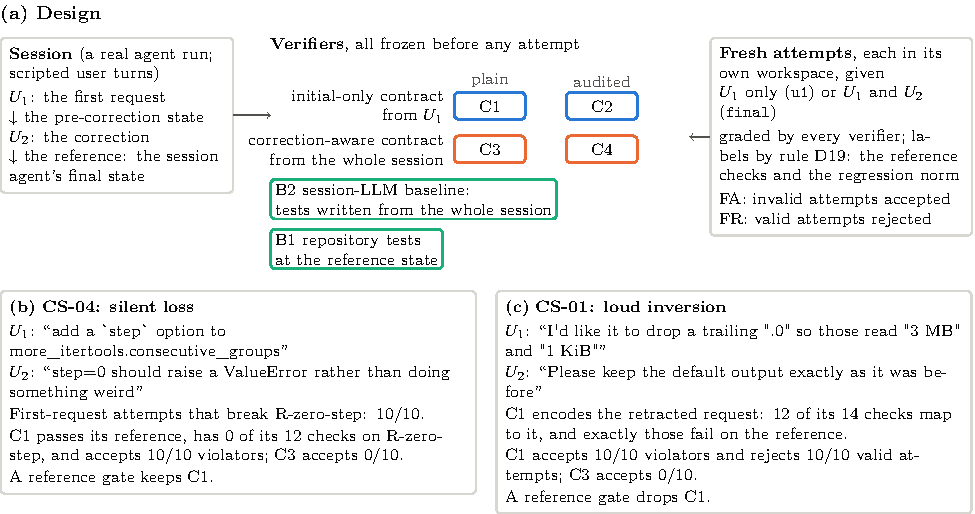
\includegraphics[width=\linewidth]{generated/figures/design_example.pdf}%
\else\unfilled{figure design\_example: main.tex must load graphicx}\fi
\caption{The design (a), and two worked examples from the fresh-agent stratum, run \texttt{fresh-v1}, under rule D19's labels and read post hoc: (b) CS-04 and (c) CS-01, each with excerpts of its first request ($U_1$) and correction ($U_2$), quoted from the synthetic scenario files. Every number in the panels is a value of Tables~\ref{tab:fresh-family}, \ref{tab:fresh-behaviours} and~\ref{tab:fresh-cv}. $^{\diamond}$Automated pilot; model-proposed labels, no human labels; 4 controlled families; descriptive (\S\ref{sec:intro}).}\label{fig:design}
\end{figure}
}{\unfilled{figure design\_example (make\_figures.py)}}

\paragraph{Findings.} Every analysed attempt that saw the correction is valid (\fv{solve.final}; \fv{attempts.excluded.w} attempt was excluded after its audit). Of the \fv{cv.attempts} that saw only the first request, \fv{u1.invalid.n} are invalid: \fv{cv.n} violate a requirement the correction introduced, and \fv{unspec.n} only break a base-commit test that the reference passes (the regression norm). The planned measure (protocol~\S15.4, estimand~3) is how C1 and C3 grade the violators: C1 accepts \fv{cv.c1}, C3 \fv{cv.c3} (\S\ref{sec:results-controlled}). Read post hoc, by behaviour, the violators show a \emph{silent loss} and a \emph{loud inversion}. In CS-03 and CS-04 the correction only adds requirements; C1 passes its reference, so a reference gate keeps it, yet it accepts \fv{cv.silent.c1} violators there (C3: \fv{cv.silent.c3}), and none of its checks maps to the requirement they break. In CS-01 the correction retracts a requirement of the first request; C1 encodes the retracted request and fails its own reference, which a gate would catch. CS-02 has no correction violator. Repository tests at the reference state cut both ways: they reject \fv{b1.fr} valid attempts, all through the tests the session agent added, and without those tests they accept \fv{b1.base.fa} invalid ones. In the natural case studies (\S\ref{sec:natural-cases}), the pre-review state, the tree a reviewer commented on and so invalid with respect to the correction under the source-evidence label, was rejected by C1 to C4 and B2 in NP-03, NP-04, NP-05, NP-18, NP-19 and NP-20; B1 accepted it in NP-03, NP-05, NP-19 and NP-20, where B1 equals the regression norm or part of it, and B3, a secondary diff-derived arm, in NP-04.

Our working hypothesis was that verifiers built from a session's final requirements, with evidence links and an audit, accept fewer violators than verifiers built from the first request. The data are consistent with the hypothesis, descriptively, for correction-aware against initial-only reconstruction on these \fv{families.w} tasks. They show no benefit of the audit, which added false rejections (C4 \fv{c4.fr} against C3 \fv{c3.fr}). On false acceptance, structured contracts did not differ from a session-LLM baseline.

\paragraph{How far the evidence goes.} This is an automated pilot: every label is a model proposal; no human label exists. Every model-written artifact comes from models of one model family of one provider, which are not named. The \fv{families.w} tasks were written by the study's own agent, and the fresh attempts add candidates, not tasks: they reuse the tasks and frozen verifiers of an earlier construction pilot (\S\ref{sec:pilot}) and were designed after its results were known. The silent-loss subset is a post hoc reading of the secondary, reference-gated view. No family-level sign-flip test over \fv{families.w} families can go below one-sided $p=\fv{cmp.floor.one}$, so every result is descriptive, and the design cannot say how often corrections are lost in practice. The natural arm, in which a reviewer's comment on an agent's pull request plays the correction, is reported as \nrv{families} exploratory case studies, family by family (\S\ref{sec:natural-cases}).

\paragraph{Contributions.} Prior work builds tasks from sessions and measures verifier errors (\S\ref{sec:related}); what we add is narrow. (a)~Withholding the correction from fresh agents, as a source of agent-made negatives that no generator wrote. (b)~How verifiers built with and without the correction grade those violators, with nulls for the audit and for structured contracts against a session-LLM baseline. (c)~The double edge of agent-added tests in repository suites taken at the reference state. (d)~Infrastructure, not a learning method: process-separated grading with isolation probes, a locally logged and hashed protocol, and an evidence-ledger entry for every number. (e)~Natural case studies from pull-request reviews, and the screening funnel behind them. No training experiment was run, and we make no claim of model improvement.

% Section 2, study design (restructure plan, part 2). Sources: experiments/protocol.md (§2, §4, §15.4, §15.5, §15.7,
% §18); docs/decision_log.md (the D-ids in the text); scripts/propose_labels.py (d19, combine_repeats; Table
% tab:label-rules); src/tracecontract/audit.py (the audit's checks and blocking findings); the generator template
% experiments/prompts/workflows/tracecontract-generate__wf_b796bb4f-1dd.js (the over-fitting sentence). Every number is a
% macro: \fv (evidence_ledger_fresh.md), \dv (evidence_ledger_design.md), \nrv (evidence_ledger_natural_run.md).
\section{Study design}
\label{sec:design}
This section describes the controlled study. The natural arm follows the same design with the differences that \S\ref{sec:natural-cases} lists, after a screening funnel of deterministic stages S1 to S8a, a model-judged stage S9 and a replay stage S10, whose families S11 accepts for building (Table~\ref{tab:natural-funnel}); each accepted family is then built in phases P0 to P7 (Appendix~\ref{app:natural}). ``Protocol~\S$n$'' refers to the locally logged protocol (\texttt{experiments/protocol.md}), and ``D$n$'' to an entry of the decision log (\texttt{docs/decision\_log.md}).

\subsection{Tasks, sessions and attempts}
\label{sec:design-tasks}
The population is controlled (protocol~\S2). Each task family is a real agent session on a pinned commit of a permissively licensed Python library, whose user turns the study's own agent wrote and hashed before the session ran (protocol CS-v1). Its feedback is therefore synthetic, and we never describe it as user traffic. A scenario fixes $U_1$, $U_2$, a neutral reply to clarification questions, and the intended requirements with the turn that introduced each (Table~\ref{tab:scenarios}). Figure~\ref{fig:design} shows the design.
\begin{itemize}
\item CS-01 (\texttt{humanize}): $U_1$ asks \texttt{naturalsize} to drop a trailing \texttt{.0}; the correction makes this opt-in and keeps the default and custom-format output, retracting part of $U_1$.
\item CS-02 (\texttt{tinydb}): atomic JSON writes; the correction adds read-after-write, unchanged bytes, no leftover temporary files and an intact original on failure.
\item CS-03 (\texttt{inflection}): \texttt{titleize} keeps acronyms; the correction keeps all-uppercase input title-cased and \texttt{humanize} and \texttt{underscore} unchanged.
\item CS-04 (\texttt{more-itertools}): \texttt{consecutive\_groups} gets a \texttt{step}; the correction adds negative steps, an error for \texttt{step=0}, positional ordering, lazy groups and an unchanged default.
\end{itemize}
The session agent, a subagent of an AI coding agent, works in a fresh git copy of the base commit and runs repository code only through wrappers that execute it in an offline sandbox. Its workspace is captured after $U_1$ (the pre-correction state) and at the end (the reference); the correction arrives through a messaging channel that adds a short harness frame (D10). We call the agent session that ran the study, and launched every other agent, the \emph{build session}. The \emph{owner} is the person who owns the study's repository and instructs the build session. A \emph{builder decision} is a choice that the build session made and logged in the decision log without the owner; the paper marks those that await the owner's review (Appendix~\ref{app:deviations}).

Fresh agents, subagents of the same AI coding agent, attempt each task in \fv{run.configurations.w} configurations, A and B (protocol~\S15.4): A is the build session's default model and B the smallest model tier the agent tool offers, \fv{run.configurations.w} model tiers of one model family of one provider. The protocol and the decision log name the agent tool but no model identifier, which the protocol keeps in private run records. The repository does name models elsewhere: each of its commit messages carries a co-author line that names a model, and its committed controlled-session transcripts carry the session agent's model identifier in their raw records (D79). The paper names no model. Configuration B also writes the independent labeler (Table~\ref{tab:roles}).

An attempt receives $U_1$ (\texttt{u1}), or $U_1$, the line ``Later in the session the user added:'' and $U_2$ (\texttt{final}), each verbatim up to recorded path substitutions (Appendix~\ref{app:deviations}), and nothing else: no reference, transcript, verifier, candidate or label (protocol~\S15.4). Each attempt works in its own workspace (a fresh git repository of the base snapshot, the instruction and the sessions' sandbox wrappers) for at most \dv{design.attempt.minutes} minutes. With $k=\dv{design.k}$ per family, variant and configuration there are \fv{attempts} attempts. An attempt's final state, without the files the patch policy removes (its test-file edits among them), is its candidate. Each transcript is audited for access outside the workspace. Under the review rule of protocol v0.10, fixed after the first family's flags had been read and before any grading, \fv{attempts.excluded.w} attempt is excluded: \texttt{\fv{excluded.1}} wrote, read and ran helper files of its own in the build session's scratch directory (D62). A sensitivity view leaves out all \fv{sens.excluded} flagged attempts (protocol~\S18.1). The attempts' context also held harness material that holds no reference, transcript, verifier, candidate or label: an environment block naming the study repository and that scratch directory, and task-list reminders with the titles (and, in CS-03 and CS-04, the descriptions) of the build session's task-list items, in the attempts whose audit records them (protocol~\S18.2; Appendix~\ref{app:deviations}).

\subsection{Verifier conditions}
\label{sec:design-conditions}
The same proposer prompt (\texttt{contract:v1}) recovers the correction-aware contract from the whole session and the initial-only contract from $U_1$ alone. Superseded and unresolved requirements are never scored. A generator writes black-box tests from a contract (the prompt asks for \dv{design.tests.min} to \dv{design.tests.max}; C1, C3 and B2 have \fv{checks.plain.min} to \fv{checks.plain.max} scored checks, Table~\ref{tab:verifiers}): C1 from the initial-only and C3 from the correction-aware contract, both single-pass. B2's generator gets the whole transcript and no contract. Every generator gets the same template (apart from the deviations of Appendix~\ref{app:deviations}), the base repository and the reference diff, with the instruction ``Do not over-fit to its particular implementation choices''. The C1--C3 contrast therefore isolates what the contract asks the generator to test, not what information reached it. B1 is the repository's tests at the reference state that pass on the reference; since the reference is the session agent's final state, they include tests that agent added. In the natural arm only, a secondary arm B3 gets the initial request and the reference diff and no contract, and keeps a test only if it fails on the base and passes on the reference (protocol~\S15.6).

C2 and C4 start from C1's and C3's tests and apply the audit (\texttt{audit:v1}), which grades audit candidates only (the development candidates, never a held-out candidate): the reference \dv{design.audit.reference.repeats.w} times, the no-op (the base snapshot unchanged), \dv{design.audit.attacks.w} attacks written from the same contract, each to violate a requirement, and \dv{design.audit.alternatives.w} valid alternative. The audit passes when the reference passes every repeat, the no-op and every attack fail, the alternative passes, every scored requirement maps to a check and a static lint passes. It also asks each attack to fail a check mapped to the requirement it targets, and reports an attack that fails only other checks as a finding that does not fail the audit. After a failing audit a reviser changes the tests, keeping \dv{design.revise.tests.min} to \dv{design.revise.tests.max} of them, at most \dv{design.audit.revisions.w} times (C2 and C4 have \fv{checks.audited.min} to \fv{checks.audited.max} scored checks), and a verifier whose audit still fails is frozen as it stands (D27). The audit's attacks come from the verifier's own contract, so it cannot supply a requirement the contract lacks, though a revision can tighten checks on behaviour the contract leaves open, as CS-03's did (\S\ref{sec:results-nulls}). Every verifier that grades the attempts, the label-support verifiers included, was frozen by content hash before the first attempt (Table~\ref{tab:roles}).

\begin{table}[t]\centering\scriptsize\setlength{\tabcolsep}{3pt}
\caption{Who wrote what. Configuration: A or B where a record holds it (A and B use different models of one model family of one provider, which are not named; protocol~\S15.4, \S15.5, \S19.2; D64); not named: a record holds the identifier, and the paper does not name it; not recorded: no record holds it, so the statement that these roles use the same model family cannot be checked from the release. Frozen before: what did not exist yet when the output was frozen.}\label{tab:roles}
\begin{tabular}{@{}>{\raggedright\arraybackslash}p{0.2\linewidth}>{\raggedright\arraybackslash}p{0.13\linewidth}>{\raggedright\arraybackslash}p{0.24\linewidth}>{\raggedright\arraybackslash}p{0.22\linewidth}>{\raggedright\arraybackslash}p{0.15\linewidth}@{}}\toprule
Role & Configuration & Inputs & Outputs & Frozen before \\\midrule
\emph{Controlled arm} & & & & \\
Scenario writer (the study's agent) & same model as the session agent & the study's design & $U_1$, $U_2$, intended requirements; the reference contract's quotes & its session (hashed) \\
Session agent & not named & $U_1$, then $U_2$; the base repository & pre-correction state, reference, transcript & --- \\
Contract proposers & not recorded & $U_1$ alone, or the whole session & initial-only and correction-aware contracts & the verifiers \\
Generators and revisers of C1--C4 and B2 & not recorded & a contract (B2: the transcript), the base repository, the reference diff; revisers: the audit's findings & tests & any held-out candidate \\
Reference-check writers & A & the reference contract, the base repository, the reference diff & reference checks & the attempts \\
Independent labeler & B & the reference contract, the base snapshot & per-requirement checks & the attempts \\
Fresh attempts & A and B & $U_1$, or $U_1$ and $U_2$; the base snapshot & attempts & --- \\
Pilot pool writers and mappers & not recorded & the reference instruction or the reference; the contracts & constructed candidates; coverage maps & --- \\\addlinespace
\emph{Natural arm} & & & & \\
S9 judges & A & a pseudonymised comment, issue and diffs & screening verdicts & --- \\
Proposers, generators, revisers, reference-contract drafter, reference-check writers and reviewers, pool writers, mappers & A & the issue or the thread, the diffs, the base repository & contracts, verifiers, reference contract and checks, held-out pool & the next phase (D64) \\
Independent labeler and its revision & B & the rendered reference contract, the base snapshot & per-requirement checks & the held-out pool \\
\bottomrule\end{tabular}\end{table}

\subsection{Labels}
\label{sec:design-labels}
The labeling standard is the reference contract plus a regression norm. A controlled reference contract states the study's intended requirements, hashed before each session ran; the study's agent operationalised it with quotes from the session, and only a model reviewed it. The label-support verifiers, which are not conditions, implement the standard.
\begin{itemize}
\item The \emph{reference checks} were written by configuration-A agents from the reference contract and validated only on the reference and the no-op. Only CS-02's went through a review-and-fix loop (D33).
\item The \emph{regression norm} is the base commit's tests that pass on the reference; a candidate that fails any of them is invalid.
\item The \emph{independent labeler} is written per family by a configuration-B agent from the reference contract and the base snapshot alone, with no reference diff, reference check, verifier, candidate or label, and no regression part (protocol~\S15.5). It gives a second labeling, reported beside the label rule's and never changing it; its agreement with the label rule is agreement between models that read the same reference contract. Like the reference checks, it was validated on the reference, which it had to pass (protocol~\S15.5) and passes in every repeat (Appendix~\ref{app:construction}), and the regression norm is the base tests that pass on the reference; so, as in the natural arm, every label source treats the session agent's final state as correct on what it tests.
\end{itemize}
The label rule labels an attempt invalid if a reference check or the regression norm fails, and valid if both pass (Table~\ref{tab:label-rules}). A violation the reference checks do not exercise is therefore labelled valid for attempts, so no verifier is charged with accepting it. The labels are not independent of the verifiers that score best: by the study's procedure, the reference checks and the correction-aware verifiers C3 and C4 are written by models of the same model family, from the same reference diff, and from requirement lists that the mappers judge to cover the same requirements (the correction-aware contracts cover every requirement of the reference contracts, Table~\ref{tab:coverage}), so their blind spots are likely correlated (Appendix~\ref{app:pilot}). That C3 and C4 accept none of the correction violators (\fv{cv.c3}, \fv{cv.c4}) is therefore partly agreement between renderings of the same requirements. No human label exists; the blinded review packet exists and has not been used.

\begin{table}[t]\centering\scriptsize
\caption{Label rules by candidate source (rule D19, \texttt{scripts/propose\_labels.py}; protocol~\S15.5, \S15.6; D64). D19 combines the reference checks, the regression norm and, for constructed candidates, the construction intent recorded when the candidate was built. An ambiguous candidate is left out of FA and FR and queued for human review.}\label{tab:label-rules}
\begin{tabular}{@{}>{\raggedright\arraybackslash}p{0.27\linewidth}>{\raggedright\arraybackslash}p{0.69\linewidth}@{}}\toprule
Candidates & Rule \\\midrule
Constructed: the pilot's alternatives and near misses; the natural pool's alternatives and near misses & Valid only if built valid and both the reference checks and the norm pass, each with a decision. Invalid only if built invalid and some reference check fails, and either a failing check maps to a targeted requirement or REGRESSION is targeted and the norm fails. Anything else is ambiguous. \\
Observed: the pilot's pre-correction states; fresh attempts & Invalid if a reference check or the norm fails; valid if both pass; ambiguous only on a missing decision. \\
Natural pre-review states & Invalid only through a failing reference check; ambiguous if the reference checks pass, whatever the norm says; never valid. \\
Every natural candidate & The reference checks and the norm are graded \dv{natural.d19.repeats.w} times; repeats that disagree make the label ambiguous, and unusable reference checks make every D19 label of the family ambiguous. \\
Second labeling (the independent labeler): attempts and natural candidates & Reported beside D19, never changing it. A labeler pass on a natural pre-review state is ambiguous; an unusable labeler is left out (NP-03, NP-19). \\
Source-evidence label: natural pre-review states & Invalid with respect to the correction, on the strength of the reviewer's request, the addressing commit and the agreement of both model judges of S9. \\
\bottomrule\end{tabular}\end{table}

\subsection{Metrics and plan}
\label{sec:design-metrics}
False acceptance is the share of invalid held-out candidates whose outcome is a pass, false rejection the share of valid ones without a pass; every other outcome counts as a rejection. Each distinct graded patch counts once: \fv{units} graded patches come from the \fv{attempts} attempts, less the excluded attempt. The unit of analysis is the task family. The \fv{cmp.count} planned paired comparisons, on FA and on FR, are C1--C3 and C2--C4 (initial-only against correction-aware), C1--C2 and C3--C4 (the audit), B2--C3 and B2--C4 (structured contract against the session-LLM baseline) and B1--C4 (repository tests). Each has an exact sign-flip p-value over families: with \fv{families.w} families there are \dv{design.signflip.assignments} sign assignments, so no p-value can fall below \fv{cmp.floor.one} one-sided or \fv{cmp.floor.two} two-sided, and a family with no difference raises the floor.

The per-family table is the primary display. The reference-gated view (the protocol's oracle-gated view), which drops a verifier in each family where it fails its own reference and reports the lost yield, is secondary; both were planned before grading (protocol v0.7, \S15.7). The silent-loss subset of \S\ref{sec:results-controlled} is a post hoc reading of that secondary view, chosen after the results and an internal review. The analysis plan is logged locally: hashed before the first evaluation run and amended \dv{protocol.amendments} times, each version hashed and timestamped (Table~\ref{tab:amendments}). \texttt{\FRESHRUN} tests, on new candidates, a design tuned on the same \fv{families.w} families.

% Section 3, controlled results (restructure plan, parts 2 and 5). Every number is a macro of
% generated/fresh/numbers.tex (\fv; evidence_ledger_fresh.md names its file and field). Sources:
% results/runs/fresh-v1/{manifest,analysis,analysis_sensitivity}.json and results.jsonl; the verifier specs and the
% contract mappings of tasks/CS-0*; data/controlled/scenarios/CS-0*.json; docs/decision_log.md D61, D62.
\section{Controlled results}
\label{sec:results-controlled}
Under D19, every analysed attempt given the correction is valid (\fv{solve.final}), and \fv{solve.u1} of those given the first request alone are (Table~\ref{tab:fresh-solve}). The \fv{u1.invalid.n} invalid first-request attempts split into \fv{cv.n} correction violators, which break a requirement the correction introduced, and \fv{unspec.n} attempts that only break a base-commit test that the reference passes (the regression norm; CS-02). Table~\ref{tab:fresh-family}, the primary display, gives false acceptance and false rejection per family, and Figure~\ref{fig:fresh-fa} draws them with the correction violators apart from the regression-only attempts; the run's bookkeeping is in the table's caption. Every rate rests on model-proposed labels.

\IfFileExists{generated/fresh/fresh_per_family.tex}{\begin{table}[t]\centering\footnotesize\setlength{\tabcolsep}{4pt}
\caption{Per-family false acceptance and false rejection on the fresh-agent stratum, the primary display (protocol \S15.7), under rule D19's labels: 29 invalid and 50 valid attempts, each distinct graded patch once (79 graded patches; excluded by the reviewed audit: \texttt{CS-02-fresh-A-final-1}). Run \texttt{fresh-v1} graded every pair 3 times under harness 0.3.5 (672 pairs, 0 unresolved). n/a: the family has no attempt of that kind. The second labeler's view: Table~\ref{tab:fresh-family-labeler}. $^{\diamond}$Automated pilot; model-proposed labels, no human labels; 4 controlled families; descriptive (\S\ref{sec:intro}).}\label{tab:fresh-family}
\begin{tabular}{lrrrrrrrrrr}\toprule  & \multicolumn{5}{c}{False acceptance (accepted/invalid)} & \multicolumn{5}{c}{False rejection (rejected/valid)} \\\cmidrule(lr){2-6}\cmidrule(lr){7-11} Condition & CS-01 & CS-02 & CS-03 & CS-04 & Pooled & CS-01 & CS-02 & CS-03 & CS-04 & Pooled \\\midrule
C1 initial-only, plain & 10/10 & 0/2 & 4/7 & 10/10 & 24/29 & 10/10 & 0/17 & 3/13 & 0/10 & 13/50 \\
C2 initial-only, audited & 10/10 & 0/2 & 4/7 & 10/10 & 24/29 & 10/10 & 0/17 & 3/13 & 0/10 & 13/50 \\
C3 correction-aware, plain & 0/10 & 2/2 & 0/7 & 0/10 & 2/29 & 0/10 & 0/17 & 0/13 & 0/10 & 0/50 \\
C4 correction-aware, audited & 0/10 & 2/2 & 0/7 & 0/10 & 2/29 & 0/10 & 0/17 & 6/13 & 0/10 & 6/50 \\
B2 session-LLM baseline & 0/10 & 2/2 & 0/7 & 0/10 & 2/29 & 0/10 & 0/17 & 2/13 & 0/10 & 2/50 \\
B1 repository tests & 0/10 & 0/2 & 0/7 & 0/10 & 0/29 & 8/10 & 17/17 & 9/13 & 0/10 & 34/50 \\
\bottomrule\end{tabular}\end{table}
}{\unfilled{per-family table (make\_tables.py -{}-fresh)}}
\IfFileExists{generated/figures/fresh_fa_fr_by_family.tex}{% Generated by `python paper/make_figures.py`; do not edit. Every value: paper/evidence_ledger_figures.md.
\begin{figure}[t]\centering
\ifdefined\includegraphics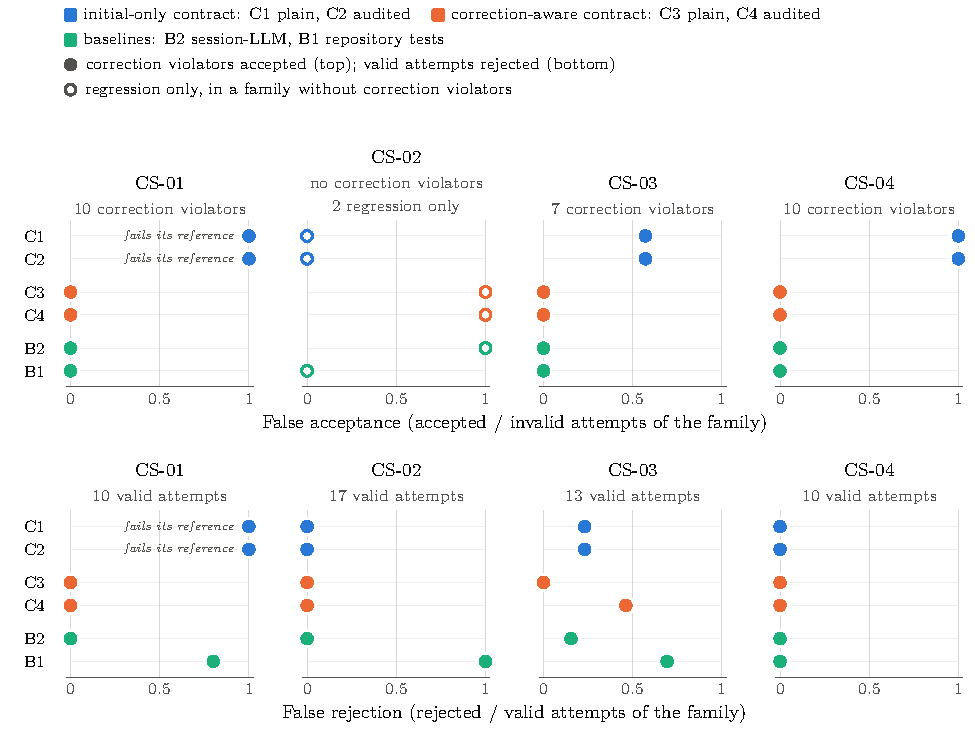
\includegraphics[width=\linewidth]{generated/figures/fresh_fa_fr_by_family.pdf}%
\else\unfilled{figure fresh\_fa\_fr\_by\_family: main.tex must load graphicx}\fi
\caption{False acceptance (top) and false rejection (bottom) per family and condition, run \texttt{fresh-v1}, under rule D19's labels, each distinct graded patch once. Filled marks: correction violators accepted, or valid attempts rejected; hollow marks: a family's invalid attempts when it has no correction violators. Colour: the contract source. Counts: Tables~\ref{tab:fresh-family} and~\ref{tab:fresh-cv}. $^{\diamond}$Automated pilot; model-proposed labels, no human labels; 4 controlled families; descriptive (\S\ref{sec:intro}).}\label{fig:fresh-fa}\label{fig:fresh-fr}
\end{figure}
}{\unfilled{figure fresh\_fa\_fr\_by\_family (make\_figures.py)}}

\subsection{The planned measure, then by behaviour}
\label{sec:results-planned}
The planned measure (protocol~\S15.4, estimand~3) is how C1 and C3 grade the correction violators: C1 accepts \fv{cv.c1} and C3 \fv{cv.c3}. C2 and C4 grade them as C1 and C3 do (\fv{cv.c2}, \fv{cv.c4}), and B2 and B1 accept none (\fv{cv.b2}, \fv{cv.b1}; Table~\ref{tab:fresh-cv}). By behaviour, in a post hoc reading of the secondary reference-gated view (protocol~\S15.7), the families differ as Table~\ref{tab:fresh-behaviours} shows.

\IfFileExists{generated/fresh/fresh_behaviours.tex}{\begin{table}[t]\centering\scriptsize\setlength{\tabcolsep}{2pt}
\caption{What the invalid first-request (\texttt{u1}) attempts of run \texttt{fresh-v1} did, by family, a post hoc reading under rule D19's labels: what the correction changed (the scenario files), which requirements the invalid attempts break (with counts), whether C1 passes the family's reference, how many of C1's checks map to the retracted requirement or to those every violator breaks (both model mappers), how many correction violators C1 and C3 accept (--: the family has none), how many invalid attempts the base-commit tests alone accept, and the invalid attempts whose only violated requirement is the regression norm (Regression only). In CS-01, R-keep-meaningful, introduced in the first request, is broken through the correction's interface: its reference statement and its checks call the correction's keyword \texttt{strip\_trailing\_zero}. $^{\diamond}$Automated pilot; model-proposed labels, no human labels; 4 controlled families; descriptive (\S\ref{sec:intro}).}\label{tab:fresh-behaviours}
\begin{tabular}{l>{\raggedright\arraybackslash}p{0.09\linewidth}>{\raggedright\arraybackslash}p{0.2\linewidth}>{\raggedright\arraybackslash}p{0.11\linewidth}>{\raggedright\arraybackslash}p{0.12\linewidth}>{\raggedright\arraybackslash}p{0.075\linewidth}>{\raggedright\arraybackslash}p{0.075\linewidth}>{\raggedright\arraybackslash}p{0.075\linewidth}>{\raggedright\arraybackslash}p{0.09\linewidth}}\toprule Family & Correction & Invalid \texttt{u1} attempts: what they break & C1 passes its reference & C1 checks on the retracted or broken requirement & C1 accepts & C3 accepts & Base tests accept & Regression only \\\midrule
CS-01 & \raggedright\hspace{0pt}adds 3, retracts 1 & \raggedright\hspace{0pt}10: R-default-unchanged, R-keep-meaningful, R-opt-in, REGRESSION (10); R-custom-format-unchanged (6) & \raggedright\hspace{0pt}no (12 of 14 checks fail) & \raggedright\hspace{0pt}12 of 14 on the retracted R-default-trim & \raggedright\hspace{0pt}10/10 & \raggedright\hspace{0pt}0/10 & \raggedright\hspace{0pt}0/10 & \raggedright\hspace{0pt}0 \tabularnewline
CS-02 & \raggedright\hspace{0pt}adds 4, retracts none & \raggedright\hspace{0pt}2: REGRESSION (2) & \raggedright\hspace{0pt}yes & \raggedright\hspace{0pt}-- & \raggedright\hspace{0pt}-- & \raggedright\hspace{0pt}-- & \raggedright\hspace{0pt}0/2 & \raggedright\hspace{0pt}2 \tabularnewline
CS-03 & \raggedright\hspace{0pt}adds 3, retracts none & \raggedright\hspace{0pt}7: R-all-caps-input (7) & \raggedright\hspace{0pt}yes & \raggedright\hspace{0pt}0 of 14 on R-all-caps-input & \raggedright\hspace{0pt}4/7 & \raggedright\hspace{0pt}0/7 & \raggedright\hspace{0pt}7/7 & \raggedright\hspace{0pt}0 \tabularnewline
CS-04 & \raggedright\hspace{0pt}adds 5, retracts none & \raggedright\hspace{0pt}10: R-zero-step (10) & \raggedright\hspace{0pt}yes & \raggedright\hspace{0pt}0 of 12 on R-zero-step & \raggedright\hspace{0pt}10/10 & \raggedright\hspace{0pt}0/10 & \raggedright\hspace{0pt}10/10 & \raggedright\hspace{0pt}0 \tabularnewline
\bottomrule\end{tabular}\end{table}
}{\unfilled{behaviours table (make\_tables.py -{}-fresh)}}

\paragraph{Silent loss (CS-03, CS-04).} In these families the correction adds \fv{corr.cs03.added.w} and \fv{corr.cs04.added.w} requirements and retracts none, and C1 \fv{ref.c1.cs03} CS-03's reference and \fv{ref.c1.cs04} CS-04's, so a reference gate keeps it. Yet it accepts \fv{cv.silent.c1} of their correction violators (\fv{cv.c1.cs03} in CS-03, \fv{cv.c1.cs04} in CS-04), against \fv{cv.silent.c3} for C3. The violators break \fv{beh.cs03.broken} in CS-03 and \fv{beh.cs04.broken} in CS-04, and no C1 check maps to that requirement (\fv{c1.cs03.checks.broken} of \fv{checks.cs03.c1} checks in CS-03, \fv{c1.cs04.checks.broken} of \fv{checks.cs04.c1} in CS-04; the second model mapper finds \fv{c1.cs03.checks.broken.mapper2} and \fv{c1.cs04.checks.broken.mapper2}). C1 is not asked to test it, and its generator is told not to over-fit the reference diff it is given. The \fv{c1.cs03.cv.rejected} CS-03 violators that C1 rejects fail checks of other requirements of its contract: \fv{c1.cs03.cv.rejected.r4} fail a check of its R4, that \texttt{titleize} behaves as before apart from acronyms, and \fv{c1.cs03.cv.rejected.r3} also a check of its R3, the general acronym rule.

\paragraph{Loud inversion (CS-01).} Here the correction retracts \fv{corr.cs01.superseded.w} requirement of the first request and adds \fv{corr.cs01.added.w} (Figure~\ref{fig:design}c). C1 encodes the retracted request: \fv{c1.cs01.checks.superseded} of its \fv{checks.cs01.c1} checks map to it (\fv{c1.cs01.checks.superseded.mapper2} for the second mapper), and exactly those fail on the reference (\fv{c1.cs01.checks.superseded.failed} of them, and \fv{c1.cs01.checks.other.failed} of the other checks). C1 accepts \fv{cv.c1.cs01} violators and rejects \fv{c1.cs01.fr} valid attempts. A reference gate drops it in CS-01: the gated view loses \fv{og.c1.lost.invalid} invalid and \fv{og.c1.lost.valid} valid attempts, and gated C1 accepts \fv{og.c1.fa} invalid attempts, a denominator that includes CS-02's \fv{unspec.n} regression-only attempts.

\paragraph{No correction violator (CS-02).} None of CS-02's first-request attempts violates the correction (\fv{cv.cs02}). Its \fv{unspec.n} regression-only attempts fail a base test that asserts on a private attribute both removed, pass all \fv{checks.cs02.ref} reference checks, and are valid for the second labeler (D62). C3, C4 and B2 accept them (\fv{unspec.c3}, \fv{unspec.c4}, \fv{unspec.b2}), and they are the whole of those verifiers' false acceptance (\fv{c3.fa}, \fv{c4.fa}, \fv{b2.fa}).

\subsection{The machinery nulls}
\label{sec:results-nulls}
C2 equals C1 on every attempt (difference \fv{cmp.c1-c2.fa.diff} on FA and \fv{cmp.c1-c2.fr.diff} on FR, with no discordant attempt), although its audit failed in CS-01 with the reference not passing, and C2 was frozen as it stood (D27). C4 equals C3 on false acceptance and rejects \fv{c4.fr} valid attempts against C3's \fv{c3.fr}, all in CS-03 (\fv{c4.cs03.fr}). There its audit made \fv{audit.c4.cs03.revisions.w} revision, which added \fv{audit.c4.cs03.added} checks that fix the answers of an audit attack, and of the reference, on edge cases the contracts leave open: contractions, digits and underscores in all-caps words. Of the rejections, \fv{c4.cs03.fr.added} fail only those checks, and the audit record shows no finding after the revision and does not show the added checks (D62). B2 matches C3 and C4 on false acceptance (\fv{b2.fa}); on false rejection it lies between them (\fv{b2.fr}, against \fv{c3.fr} and \fv{c4.fr}). No difference was observed on false acceptance, and \fv{families.w} families cannot show equivalence.

None of the \fv{cmp.count} planned comparisons reaches the unconditional floor of the family-level sign-flip test (\fv{cmp.floor.one} one-sided, \fv{cmp.floor.two} two-sided; Table~\ref{tab:fresh-comparisons}). C1 against C3 on false acceptance (\fv{cmp.c1-c3.fa.diff}) has one-sided $p=\fv{cmp.c1-c3.fa.p.greater}$, above its floor of \fv{cmp.c1-c3.fa.floor}, because CS-02 differs in the other direction (\fv{cmp.c1-c3.fa.cs02}). C1 against C3 and B1 against C4 on false rejection sit at their conditional floors (\fv{cmp.c1-c3.fr.floor} and \fv{cmp.b1-c4.fr.floor}), which the families with no difference set.

\IfFileExists{generated/fresh/fresh_comparisons.tex}{\begin{table}[t]\centering\scriptsize\setlength{\tabcolsep}{4pt}
\caption{The 14 pre-specified paired comparisons on the same units, run \texttt{fresh-v1}, D19 labels. \textbf{All labels are model proposals; no human labels exist.} Metric (n): FA over the invalid or FR over the valid units. A$-$B: pooled difference; then the per-family differences. Disc.: A accepts \& B rejects / A rejects \& B accepts. $p$: exact sign-flip randomization p-values over the 4 families, on the pooled statistic ($>$: A$>$B, $<$: A$<$B, both one-sided; 2-s.: two-sided) and, last but one, two-sided on the family-mean statistic. With 4 families no one-sided $p$ below 0.0625 and no two-sided $p$ below 0.125 can occur; Floor: the smallest one-sided $p$ attainable given the families whose difference is zero. The smallest two-sided $p$ here is 0.25. Short names: C1--C4 contracts (initial or full, plain or audited), B2 full-session LLM, B1 repository tests. Four controlled families: descriptive, not inferential.}\label{tab:fresh-comparisons}
\begin{tabular}{lllrrrrrrrrrrr}\toprule A & B & Metric (n) & A$-$B & CS-01 & CS-02 & CS-03 & CS-04 & Disc. & $p_{>}$ & $p_{<}$ & $p$ 2-s. & $p$ 2-s.\ (mean) & Floor \\\midrule
C1 & C3 & FA (29) & \ensuremath{+}0.76 & \ensuremath{+}1.00 & \ensuremath{-}1.00 & \ensuremath{+}0.57 & \ensuremath{+}1.00 & 24/2 & 0.125 & 0.9375 & 0.25 & 0.625 & 0.0625 \\
C1 & C3 & FR (50) & \ensuremath{+}0.26 & \ensuremath{+}1.00 & 0.00 & \ensuremath{+}0.23 & 0.00 & 0/13 & 0.25 & 1 & 0.5 & 0.5 & 0.25 \\
C2 & C4 & FA (29) & \ensuremath{+}0.76 & \ensuremath{+}1.00 & \ensuremath{-}1.00 & \ensuremath{+}0.57 & \ensuremath{+}1.00 & 24/2 & 0.125 & 0.9375 & 0.25 & 0.625 & 0.0625 \\
C2 & C4 & FR (50) & \ensuremath{+}0.14 & \ensuremath{+}1.00 & 0.00 & \ensuremath{-}0.23 & 0.00 & 5/12 & 0.5 & 0.75 & 1 & 1 & 0.25 \\
C1 & C2 & FA (29) & 0.00 & 0.00 & 0.00 & 0.00 & 0.00 & 0/0 & 1 & 1 & 1 & 1 & 1 \\
C1 & C2 & FR (50) & 0.00 & 0.00 & 0.00 & 0.00 & 0.00 & 0/0 & 1 & 1 & 1 & 1 & 1 \\
C3 & C4 & FA (29) & 0.00 & 0.00 & 0.00 & 0.00 & 0.00 & 0/0 & 1 & 1 & 1 & 1 & 1 \\
C3 & C4 & FR (50) & \ensuremath{-}0.12 & 0.00 & 0.00 & \ensuremath{-}0.46 & 0.00 & 6/0 & 1 & 0.5 & 1 & 1 & 0.5 \\
B2 & C4 & FA (29) & 0.00 & 0.00 & 0.00 & 0.00 & 0.00 & 0/0 & 1 & 1 & 1 & 1 & 1 \\
B2 & C4 & FR (50) & \ensuremath{-}0.08 & 0.00 & 0.00 & \ensuremath{-}0.31 & 0.00 & 4/0 & 1 & 0.5 & 1 & 1 & 0.5 \\
B2 & C3 & FA (29) & 0.00 & 0.00 & 0.00 & 0.00 & 0.00 & 0/0 & 1 & 1 & 1 & 1 & 1 \\
B2 & C3 & FR (50) & \ensuremath{+}0.04 & 0.00 & 0.00 & \ensuremath{+}0.15 & 0.00 & 0/2 & 0.5 & 1 & 1 & 1 & 0.5 \\
B1 & C4 & FA (29) & \ensuremath{-}0.07 & 0.00 & \ensuremath{-}1.00 & 0.00 & 0.00 & 0/2 & 1 & 0.5 & 1 & 1 & 0.5 \\
B1 & C4 & FR (50) & \ensuremath{+}0.56 & \ensuremath{+}0.80 & \ensuremath{+}1.00 & \ensuremath{+}0.23 & 0.00 & 0/28 & 0.125 & 1 & 0.25 & 0.25 & 0.125 \\
\bottomrule\end{tabular}\end{table}
}{\unfilled{comparisons table (make\_tables.py -{}-fresh)}}

\subsection{Repository tests cut both ways}
\label{sec:results-b1}
B1 accepts no invalid attempt (\fv{b1.fa}) and rejects \fv{b1.fr} valid ones. All \fv{b1.fr.added} rejections come from the \fv{b1.checks.added} checks that the session agent added to the reference state's test files; the base commit's \fv{b1.checks.base} checks reject none (\fv{b1.base.fr}; Table~\ref{tab:fresh-b1}). On the base-commit checks alone, B1 would accept \fv{b1.base.fa} invalid attempts (CS-03 \fv{b1.base.fa.cs03}, CS-04 \fv{b1.base.fa.cs04}) and still reject every CS-01 violator (\fv{b1.u1.base.rejected.cs01}). That last part holds partly by construction: the base tests are D19's regression norm, so under D19 they cannot reject a valid attempt, and REGRESSION is among the requirements that every CS-01 violator breaks (\fv{beh.cs01.regression} of \fv{beh.cs01.n}; D62). B1's result concerns agent-written tests carried into the reference, not repository tests in general.

\subsection{Robustness}
\label{sec:results-robust}
The second labeler agrees with D19 on \fv{agree} graded patches ($\kappa=\fv{kappa}$; Table~\ref{tab:fresh-agree}). This is agreement between models of the same model family (configurations B and A), working from the same reference contract, over attempts that cluster into a few behaviours per family. Its \fv{disagree} disagreements are CS-02's regression-only attempts, which it labels valid; under its labels C1 accepts \fv{il.c1.fa} invalid attempts and C3 \fv{il.c3.fa} (Table~\ref{tab:fresh-family-labeler}). Leaving out every flagged attempt (\fv{sens.excluded}; Table~\ref{tab:fresh-sensitivity}), C1 accepts \fv{sens.cv.c1} of the correction violators left and C3 \fv{sens.cv.c3}. The reference-gated view drops C1 in CS-01 only (\fv{og.c1.kept} families kept); there the C1--C3 difference in false acceptance is \fv{og.cmp.c1-c3.fa.diff} over \fv{og.cmp.c1-c3.fa.k} families, with one-sided $p=\fv{og.cmp.c1-c3.fa.p.greater}$ (floor \fv{og.cmp.c1-c3.fa.floor}; Table~\ref{tab:fresh-oracle}). The attempts' solve rates and costs are in Tables~\ref{tab:fresh-solve} and~\ref{tab:fresh-costs}; the cost of generating the verifiers was not recorded (D42).

% Section 4, what the construction pilot adds (restructure plan, part 2). Every number is a macro of
% generated/pilot/numbers.tex (\plv; evidence_ledger_pilot.md names its file and field): the frozen run
% results/runs/pilot-v0.3.3 and the exploratory re-analysis results/analyses/pilot-v0.3.3-exploratory (D49).
\section{What the construction pilot adds}
\label{sec:pilot}
The construction pilot (run \texttt{\PILOTRUN}) graded the same frozen verifiers on a constructed held-out pool of the same \plv{run.families.w} families: each family's pre-correction state, valid alternatives written without the reference diff, and near misses built from the reference to violate a targeted requirement (Tables~\ref{tab:summary} and~\ref{tab:labels}). Of its \plv{heldout} held-out candidates, the label rule labels \plv{labels.invalid} invalid, \plv{labels.valid} valid and \plv{labels.ambiguous} ambiguous. It adds the following, and no more.
\begin{itemize}
\item \emph{The same ordering.} C1 accepts \plv{c1.fa} invalid candidates and C3 \plv{c3.fa}.
\item \emph{The audit's \plv{audit.changed.n.w} change.} Across the held-out outcomes of the revised verifiers, the audit changed \plv{audit.changed.n.w}: C2 rejects an \texttt{inflection} near miss that C1 accepts (C1 \plv{c1.fa}, C2 \plv{c2.fa}), the only false acceptance that the audit removed in the controlled tasks (Appendix~\ref{app:pilot}).
\item \emph{The label rule's selection effect (exploratory).} The reference checks confirm \plv{nm.confirmed} of the \plv{nm.n} near misses as invalid; the other \plv{nm.ambiguous} are ambiguous and left out. C3 accepts \plv{nm.conf.c3} of the confirmed near misses but \plv{nm.amb.c3} of the unconfirmed ones (C4: \plv{nm.conf.c4} and \plv{nm.amb.c4}), and under construction-intent labels C3 accepts \plv{intent.c3.fa} invalid candidates. The zeros of \S\ref{sec:results-controlled} therefore hold only for what the reference checks exercise.
\item \emph{It is not independent evidence.} The pilot shares the tasks and the frozen verifiers with \texttt{\FRESHRUN}, which was designed after the pilot's results were known.
\item \emph{An exploratory sign-flip analysis exists} (D49). On false acceptance, C1 against C3 has one-sided $p=\plv{signflip.c1-c3.fa.p1}$ and two-sided $p=\plv{signflip.c1-c3.fa.p2}$, at its conditional floor of \plv{signflip.c1-c3.fa.floor}.
\end{itemize}
The pilot's tables, its duplicated candidates, its reliability re-grade and its cases are in Appendix~\ref{app:pilot}.

% Natural case studies: the template of the restructured manuscript's natural section (restructure plan, part 7), fixed
% before any analysis of natural-pr-v1 exists, so that its wording presupposes no outcome of the run.
% * Every value is a macro: \nrv{key} of generated/natural_run/numbers.tex (paper/make_tables.py --natural-run; ledger
%   paper/evidence_ledger_natural_run.md) or \nat{key} of generated/natural/numbers.tex (--natural; ledger
%   paper/evidence_ledger_natural.md). A key that is not generated yet prints UNFILLED.
% * Every statement cites the decision-log entry or the protocol section it comes from.
% * Premises: the fixed sentences state construction facts that the run's analysis also computes (the run's families,
%   invocations, revision and pilot flag; B1 against the regression norm; the labelers; the reference checks' fix
%   rounds; the failed audits). tests/test_natural_template.py (PREMISES) checks them on the synthetic world and, once it
%   exists, on the run's own numbers.tex. A premise the run does not bear out means that the sentence is rewritten from
%   the records, never that a cell is changed. The fix rounds are read from each reference-check status record's integer
%   fix_rounds, a key D64 does not fix: the build session confirms that the six records hold it before the run is
%   analysed, since the published analysis is a byte copy (scripts/publish_natural_run.py).
% * Families are named, never counted; no thread text, repository name, login or agent product is written.
% * main.tex inputs this file as the manuscript's natural section (the restructure). Its only pointers outside itself,
%   its generated tables and its part in App. G are the two that D77 left open, re-added once the appendix moves gave
%   them their content (App. A's generated table of amendments, its v0.12 row, and App. G's comparison of the natural arm
%   with the controlled study), and the controlled study's coverage table, to which the reading with the gate points.
% * Its part in App. G is paper/sections/app_natural_cases.tex (D80): what was moved there unchanged, so that the
%   main-text section stays short. Every rule of this header holds for it, and tests/test_natural_template.py reads both.
% * What changed after the run's analysis (D79): (1) the closing paragraph's integration slot, replaced by the one
%   sentence its rule asks for, the only text of the template written from the run's cells (the abstract's, the
%   introduction's and the discussion's sentences on the case studies, outside the template, were written after the
%   analysis too; D80); (2) the two pointers above; (3) review corrections of statements about the records, none of
%   which states an outcome of the run: what was fixed before the analysis and what the build session had seen (Status),
%   the caveat on D70's construction facts and the wording of the task-list exposure (Caveats), NP-05's correction as a
%   builder default and NP-20's near-miss disclosure as D77 records it (their paragraphs), and the planned cost per
%   accepted task, not reported (closing paragraph).
% * What changed in the next round after the analysis (D80): (4) the slot, rewritten with the gate's marker that Table
%   tab:nr-source now carries, by D77's rule (one sentence per pattern of the C1 and C3 cells, each family named once);
%   (5) the new paragraph that reads the families with the reference gate, and the pointer to the coverage table; (6) the
%   Status paragraph's last sentences; (7) moved unchanged to App. G (app_natural_cases.tex): the caveats on the build's
%   process, Table tab:nr-caveats, the sentence that names the parts of a family paragraph, the family paragraphs and the
%   cost per family, with new sentences that point to them; (8) where the records contradict the text: the closing
%   paragraph's "no statement here counts families", which its own screening count of S10 contradicts, now reads "by
%   their outcomes in the run"; and an added sentence after the caveat on the generators' training data, which the
%   paper cannot check.
% * What changed in a later round (D82): (9) moved unchanged to App. G (app_natural_cases.tex), so that the main text
%   carries no run bookkeeping: the Status paragraph's sentence on the run's start and end times, invocations and code
%   revision, with D76's account of the stopped first invocation, now the paragraph "The run's dates and invocations."
%   there; a new sentence in its place points to it, and App. G's first paragraph names it.
\providecommand{\nrcaveat}[1]{\raggedright\hspace{0pt}#1}

\section{Natural case studies}
\label{sec:natural-cases}

\paragraph{Status.}
The run \texttt{\NATURALRUN} graded the \nrv{families} accepted families of the first sample (\nrv{run.families}) under
harness \nrv{run.harness}: each family's frozen verifiers (C1 to C4, B1, B2, B3 and the reference checks) and its
independent labeler on every held-out candidate, each pair \nrv{run.repeats} times (protocol~\S20.2; D76). Its start
and end times, invocations and code revision, as its manifest records them, are in Appendix~\ref{app:natural-cases}
(D82). It is an automated
pilot: provenance eligibility needs a human reviewer and stays pending, so each family's acceptance gate is pending, and
the manifest's pilot flag is \nrv{run.pilot} (D64, decision~9; D75; D76). Protocol v0.12 (protocol~\S20) gave each
sample a run of its own after phases P1 to P4 of the first sample's families had run and before any natural held-out
candidate existed (D71; Table~\ref{tab:amendments}, its v0.12 row). When this run started, the extension's run,
\texttt{natural-pr-v2}, had not been made: the extension's S10 step was stopped at a usage limit, and the task
directories it left are to be built again from the start (D66, D75), with the results of this run known
(protocol~\S20.3). This section's wording and the run's analysis fields were fixed before any analysis of the run, while
grading was still in progress; before then, the build session's progress checks had shown it counts of outcomes over all
graded pairs together, naming no verifier or candidate (D77). After the analysis, the opening of the closing paragraph
was written from the run's cells, and review corrected or added statements about the records in this section, none of
which states an outcome of the run (D79). The sentences on these case studies in the abstract, the introduction and the
discussion were also written after the analysis, from the run's cells. A later round rewrote that opening with the
reference gate, added the reading of the families with it, and moved the family paragraphs and other detail of this
section, unchanged, to Appendix~\ref{app:natural-cases} (D80).

\paragraph{What was built.}
Each family follows the recipe of D64 in phases P0 to P7, and the end of each of P1 to P7 is a committed record (D65,
D74). The generated verifiers are built and frozen in P2 and P3. The reference contract is drafted in P4, after them, so
no generator saw it, and before the reference checks and the independent labeler of P5. The held-out pool of P6,
alternatives and near misses with a workspace each, starts after every verifier of its family is frozen, and P7 runs the
mappers, the duplicate check and the audits (D64; D72; D75). A family accepted at S11 is accepted for building: it passes
S10 within the family cap (protocol~\S16.4). The natural arm differs from the controlled study in these respects
(Table~\ref{tab:natural-vs-controlled}, Appendix~\ref{app:natural}):
\begin{enumerate}
\item The correction is a reviewer's comment on an agent's pull request. The reviewer need not be the person who opened
  the issue: we treat the comment as the correction, a construct difference from an in-session user correction (D64,
  decision~1).
\item The initial request is the linked issue, the pre-correction state is the tree the reviewer commented on (the
  pre-review state), and the reference is the addressing commit, which is evidence about the correction rather than an
  oracle (protocol~\S15.6; D70).
\item A configuration-A agent drafts the reference contract in P4 from the rendered thread and the addressing diff, and
  also from the reference diff, which adds the part of the change made before the review (D64, deviation~(k)).
\item Labels: D19, whose reference checks and regression norm are graded repeatedly on each candidate, a label being
  ambiguous where the repeats disagree (D64, decision~7); the source-evidence label of the pre-review states, the label
  of the first estimand of protocol~\S15.6 (D64, decision~14); and the independent labeler, a second labeling
  (protocol~\S15.5).
\item The audit holds the reference to be valid (D24, D27), so the natural C2 and C4 are audited against an unreliable
  oracle (D70). B1 equals D19's regression norm in NP-03, NP-05 and NP-20, and in part in NP-19 (D64, decision~3). B3
  is a secondary arm (protocol~\S15.6).
\end{enumerate}

\paragraph{Caveats.}
These hold for every number of this section and of its tables, whose captions point here with the marker
$^{\ddagger}$.
\begin{itemize}
\item The reference is not an oracle, and the reference checks were validated on it: they are usable only where the
  reference passes them in every repeat of their validation and the development no-op fails them (D64; D70).
\item The construction facts that the family paragraphs take from D70, such as why a reference fails a verifier or what
  revisers relaxed, are observations of the build made by model agents and not reviewed by a person (D70).
\item Every label is a model proposal: D19's, the independent labeler's, and the source-evidence label, which rests on
  the reviewer's request, the addressing commit and the agreement of the model judges of S9 (protocol~\S15.6). No human
  label exists (D64, decision~8).
\item The independent labelers of NP-03 and NP-19 are unusable, so the second labeling leaves them out (D72, D75, D76).
\item A candidate that D19 labels ambiguous is left out of false acceptance and false rejection, and is queued for human
  review (D19; D76).
\item The run is an automated pilot, as the status paragraph says (D64, decision~9; D76).
\item Caveats on how the families were built hold here too and are listed in Appendix~\ref{app:natural-cases}:
  the run's first step, the agents' context, and the runs that worked outside the recipe.
\item The run grades \nrv{accepted} accepted tasks of its own, fewer than \nrv{threshold}, so its families are
  exploratory case studies, each reported on its own, in per-family tables only, with no pooled rate, interval or
  p-value (protocol~\S19.6, \S20.3). Nor do we give a total over the families, or pool anything with the controlled arm
  (protocol~\S2).
\item The results of this run will be known when the extension's families are built; this is disclosed with the results
  of \texttt{natural-pr-v2} (protocol~\S20.3).
\item The construct differs from an in-session correction, as the first item of the list above says (D64, decision~1).
\item The pull requests and their repositories predate the generators' training data, so public merged fixes may be
  memorised (protocol~\S15.6). The protocol states this order of dates; no model identifier is named, so the paper
  cannot check it.
\item NP-04 and NP-05 come from the same repository (D63; the committed index's repository ids).
\end{itemize}

\paragraph{Reading the tables and the family paragraphs.}
Table~\ref{tab:nr-caveats} gives each family's caveats as values of the run's analysis, Table~\ref{tab:nr-source}
which conditions accept each family's pre-review state under the source-evidence label, and Table~\ref{tab:nr-fa-fr}
false acceptance and false rejection per condition under D19. Below, false acceptance is written accepted/invalid and
false rejection rejected/valid, under D19's labels, each distinct graded patch once (protocol~\S15.7); the pre-review
state counts under its D19 label, since Table~\ref{tab:nr-fa-fr} leaves out only the reference and the no-op. The
secondary oracle-gated view keeps a verifier's cell where the verifier passes the family's reference in the run and
drops it otherwise, a $^{\dagger}$ in Table~\ref{tab:nr-fa-fr} (protocol~\S15.7). Table~\ref{tab:nr-source} marks
the same cells, Table~\ref{tab:nr-sanity} gives each condition's outcome on the reference and on the no-op, the
unchanged base, and Table~\ref{tab:nr-coverage} how much of the reference contract each recovered contract covers, how
many of its requirements contradict the reference contract, and how many it marks superseded.
The family paragraphs, which set each family's cells beside its construction facts, its second labeling, its pairs and
its own caveats, are in Appendix~\ref{app:natural-cases}, with Table~\ref{tab:nr-caveats}.

\IfFileExists{generated/natural_run/natural_run_source_evidence.tex}{\begin{table}[t]\centering\footnotesize
\caption{Acceptance of each family's pre-review state, the tree the reviewer commented on before the correction, by condition, under the source-evidence label: invalid with respect to the correction, on the strength of the reviewer's request, the addressing commit and the agreement of both S9 judges (protocol \S15.6), so an accepted state is a false acceptance under this labeling. \textbf{Source evidence, not a human label}, reported apart from D19; D19's labels and the second labeling are model proposals, and no human labels exist. Run \texttt{natural-pr-v1} in case-study mode, as exploratory case studies (protocol \S19.6, \S20.3): the run grades 6 accepted tasks of its own (its families accepted in the committed index), fewer than 10, and each run is reported on its own, so every number is per family. Nothing is pooled over the families: no pooled rate, no interval and no p-value. Below the conditions: the same state's D19 label (ambiguous where its reference checks pass it, \S15.6), its label in the second labeling with the independent labeler's outcome (a pass on a pre-review state is ambiguous, decision log D64; left out: the family's labeler is not usable), and the reference checks' outcome on it in the run. A rejection is any outcome other than a pass: one that is not a task failure (an infrastructure outcome, or an unresolved pair whose repeats disagree, protocol \S15.3) is named in brackets. Terms: --: the run did not grade the condition for the family; not graded: the run did not grade the state with that verifier; none: no label (no D19 proposal, or no label in the second labeling). $^{\ddagger}$Natural case study; caveats in Section~\ref{sec:natural-cases}.}\label{tab:nr-source}
\begin{tabular}{p{0.25\linewidth}p{0.093\linewidth}p{0.093\linewidth}p{0.093\linewidth}p{0.093\linewidth}p{0.093\linewidth}p{0.093\linewidth}}\toprule Condition & NP-03 & NP-04 & NP-05 & NP-18 & NP-19 & NP-20 \\\midrule
\raggedright\hspace{0pt}C1 initial, plain & \raggedright\hspace{0pt}rejected & \raggedright\hspace{0pt}rejected & \raggedright\hspace{0pt}rejected & \raggedright\hspace{0pt}rejected & \raggedright\hspace{0pt}rejected & \raggedright\hspace{0pt}rejected \tabularnewline
\raggedright\hspace{0pt}C2 initial, audited & \raggedright\hspace{0pt}rejected & \raggedright\hspace{0pt}rejected & \raggedright\hspace{0pt}rejected & \raggedright\hspace{0pt}rejected & \raggedright\hspace{0pt}rejected & \raggedright\hspace{0pt}rejected \tabularnewline
\raggedright\hspace{0pt}C3 full, plain & \raggedright\hspace{0pt}rejected & \raggedright\hspace{0pt}rejected & \raggedright\hspace{0pt}rejected & \raggedright\hspace{0pt}rejected & \raggedright\hspace{0pt}rejected & \raggedright\hspace{0pt}rejected \tabularnewline
\raggedright\hspace{0pt}C4 full, audited & \raggedright\hspace{0pt}rejected & \raggedright\hspace{0pt}rejected & \raggedright\hspace{0pt}rejected & \raggedright\hspace{0pt}rejected & \raggedright\hspace{0pt}rejected & \raggedright\hspace{0pt}rejected \tabularnewline
\raggedright\hspace{0pt}B2 full-session LLM & \raggedright\hspace{0pt}rejected & \raggedright\hspace{0pt}rejected & \raggedright\hspace{0pt}rejected & \raggedright\hspace{0pt}rejected & \raggedright\hspace{0pt}rejected & \raggedright\hspace{0pt}rejected \tabularnewline
\raggedright\hspace{0pt}B1 repository tests & \raggedright\hspace{0pt}accepted & \raggedright\hspace{0pt}rejected & \raggedright\hspace{0pt}accepted & \raggedright\hspace{0pt}rejected & \raggedright\hspace{0pt}accepted & \raggedright\hspace{0pt}accepted \tabularnewline\midrule
\raggedright\hspace{0pt}B3 diff-derived (secondary) & \raggedright\hspace{0pt}rejected & \raggedright\hspace{0pt}accepted & \raggedright\hspace{0pt}rejected & \raggedright\hspace{0pt}rejected & \raggedright\hspace{0pt}rejected & \raggedright\hspace{0pt}rejected \tabularnewline\midrule
\raggedright\hspace{0pt}Its D19 label & \raggedright\hspace{0pt}invalid & \raggedright\hspace{0pt}invalid & \raggedright\hspace{0pt}invalid & \raggedright\hspace{0pt}invalid & \raggedright\hspace{0pt}invalid & \raggedright\hspace{0pt}invalid \tabularnewline
\raggedright\hspace{0pt}Its second label (the labeler's outcome) & \raggedright\hspace{0pt}left out & \raggedright\hspace{0pt}invalid (task failure) & \raggedright\hspace{0pt}invalid (task failure) & \raggedright\hspace{0pt}invalid (task failure) & \raggedright\hspace{0pt}left out & \raggedright\hspace{0pt}invalid (task failure) \tabularnewline
\raggedright\hspace{0pt}The reference checks' outcome on it & \raggedright\hspace{0pt}task failure & \raggedright\hspace{0pt}task failure & \raggedright\hspace{0pt}task failure & \raggedright\hspace{0pt}task failure & \raggedright\hspace{0pt}task failure & \raggedright\hspace{0pt}task failure \tabularnewline
\bottomrule\end{tabular}\end{table}
}{\unfilled{table of the pre-review states (make\_tables.py -{}-natural-run)}}
\IfFileExists{generated/natural_run/natural_run_fa_fr.tex}{\begin{table}[t]\centering\scriptsize\setlength{\tabcolsep}{4pt}
\caption{False acceptance $\cdot$ false rejection per family and condition, as accepted/invalid $\cdot$ rejected/valid, under D19's model-proposed labels, each distinct graded patch once; the reference solution and the no-op are excluded. A rejection is any outcome other than a pass, so an infrastructure outcome (environment failure, verifier error or timeout) and an unresolved pair (repeats that disagree, protocol \S15.3) count as rejections. Below the conditions: the family's pairs graded in the run (every verifier and candidate, label support included), those unresolved, and those that ended in an infrastructure outcome. \textbf{All labels are model proposals; no human labels exist.} Run \texttt{natural-pr-v1} in case-study mode, as exploratory case studies (protocol \S19.6, \S20.3): the run grades 6 accepted tasks of its own (its families accepted in the committed index), fewer than 10, and each run is reported on its own, so every number is per family. Nothing is pooled over the families: no pooled rate, no interval and no p-value. B3 (diff-derived) is a secondary arm (protocol \S15.6). n/a: the family has no unit of that kind under D19. --: the run did not grade the condition for the family, or the analysis does not hold the value. none: no such pair. $^{\dagger}$: the verifier does not pass the family's reference solution in the run, so the secondary oracle-gated view (protocol \S15.7) drops the cell and counts its units as lost yield. $^{\ddagger}$Natural case study; caveats in Section~\ref{sec:natural-cases}.}\label{tab:nr-fa-fr}
\begin{tabular}{p{0.2\linewidth}p{0.112\linewidth}p{0.112\linewidth}p{0.112\linewidth}p{0.112\linewidth}p{0.112\linewidth}p{0.112\linewidth}}\toprule Condition & NP-03 & NP-04 & NP-05 & NP-18 & NP-19 & NP-20 \\\midrule
\raggedright\hspace{0pt}C1 initial-only, plain & \raggedright\hspace{0pt}0/3 $\cdot$ 2/2$^{\dagger}$ & \raggedright\hspace{0pt}3/4 $\cdot$ 0/1 & \raggedright\hspace{0pt}0/3 $\cdot$ 2/2$^{\dagger}$ & \raggedright\hspace{0pt}0/4 $\cdot$ 2/2$^{\dagger}$ & \raggedright\hspace{0pt}2/4 $\cdot$ 0/2$^{\dagger}$ & \raggedright\hspace{0pt}0/3 $\cdot$ 2/2$^{\dagger}$ \tabularnewline
\raggedright\hspace{0pt}C2 initial-only, audited & \raggedright\hspace{0pt}1/3 $\cdot$ 2/2 & \raggedright\hspace{0pt}3/4 $\cdot$ 0/1 & \raggedright\hspace{0pt}1/3 $\cdot$ 0/2 & \raggedright\hspace{0pt}0/4 $\cdot$ 0/2 & \raggedright\hspace{0pt}1/4 $\cdot$ 0/2 & \raggedright\hspace{0pt}1/3 $\cdot$ 0/2 \tabularnewline
\raggedright\hspace{0pt}C3 correction-aware, plain & \raggedright\hspace{0pt}0/3 $\cdot$ 2/2$^{\dagger}$ & \raggedright\hspace{0pt}2/4 $\cdot$ 0/1 & \raggedright\hspace{0pt}0/3 $\cdot$ 2/2$^{\dagger}$ & \raggedright\hspace{0pt}0/4 $\cdot$ 2/2$^{\dagger}$ & \raggedright\hspace{0pt}1/4 $\cdot$ 0/2$^{\dagger}$ & \raggedright\hspace{0pt}0/3 $\cdot$ 0/2 \tabularnewline
\raggedright\hspace{0pt}C4 correction-aware, audited & \raggedright\hspace{0pt}0/3 $\cdot$ 2/2$^{\dagger}$ & \raggedright\hspace{0pt}2/4 $\cdot$ 0/1 & \raggedright\hspace{0pt}0/3 $\cdot$ 0/2 & \raggedright\hspace{0pt}0/4 $\cdot$ 0/2 & \raggedright\hspace{0pt}1/4 $\cdot$ 0/2$^{\dagger}$ & \raggedright\hspace{0pt}0/3 $\cdot$ 0/2 \tabularnewline
\raggedright\hspace{0pt}B2 session-LLM baseline & \raggedright\hspace{0pt}0/3 $\cdot$ 0/2 & \raggedright\hspace{0pt}1/4 $\cdot$ 0/1 & \raggedright\hspace{0pt}0/3 $\cdot$ 0/2 & \raggedright\hspace{0pt}0/4 $\cdot$ 0/2 & \raggedright\hspace{0pt}1/4 $\cdot$ 0/2 & \raggedright\hspace{0pt}0/3 $\cdot$ 0/2 \tabularnewline
\raggedright\hspace{0pt}B1 repository tests & \raggedright\hspace{0pt}3/3 $\cdot$ 0/2 & \raggedright\hspace{0pt}3/4 $\cdot$ 0/1 & \raggedright\hspace{0pt}3/3 $\cdot$ 0/2 & \raggedright\hspace{0pt}1/4 $\cdot$ 0/2 & \raggedright\hspace{0pt}4/4 $\cdot$ 0/2 & \raggedright\hspace{0pt}3/3 $\cdot$ 0/2 \tabularnewline\midrule
\raggedright\hspace{0pt}B3 diff-derived (secondary) & \raggedright\hspace{0pt}1/3 $\cdot$ 0/2 & \raggedright\hspace{0pt}4/4 $\cdot$ 0/1 & \raggedright\hspace{0pt}0/3 $\cdot$ 0/2 & \raggedright\hspace{0pt}0/4 $\cdot$ 0/2 & \raggedright\hspace{0pt}2/4 $\cdot$ 0/2 & \raggedright\hspace{0pt}1/3 $\cdot$ 0/2 \tabularnewline\midrule
\raggedright\hspace{0pt}The run's pairs: graded, unresolved & \raggedright\hspace{0pt}72, 0 & \raggedright\hspace{0pt}72, 0 & \raggedright\hspace{0pt}72, 0 & \raggedright\hspace{0pt}72, 0 & \raggedright\hspace{0pt}72, 0 & \raggedright\hspace{0pt}72, 0 \tabularnewline
\raggedright\hspace{0pt}The run's pairs ending in an infrastructure outcome & \raggedright\hspace{0pt}none & \raggedright\hspace{0pt}none & \raggedright\hspace{0pt}none & \raggedright\hspace{0pt}none & \raggedright\hspace{0pt}none & \raggedright\hspace{0pt}none \tabularnewline
\bottomrule\end{tabular}\end{table}
}{\unfilled{table of false acceptance and false rejection (make\_tables.py -{}-natural-run)}}

\paragraph{The families read with the reference gate.}
% Written after the analysis, from the run's cells (D80): outside the template's
% pre-commitment. tests/test_natural_template.py (READING_CELLS, READING_ORDER) checks each family it names against the
% run's own numbers and the published analysis.
A rejection of the pre-review state tells that state from the reference only where the verifier passes the reference,
and from valid work only where it also passes the valid alternatives; an acceptance says more than the base's only where
the verifier rejects the no-op. In NP-03, C1, C3 and C4 reject every candidate, the reference and both valid
alternatives included, and so do C1 and C3 in NP-05 and NP-18, and C1 in NP-20: their rejections of the pre-review state
there carry no information about the correction. In NP-03, NP-05, NP-19 and NP-20, B1 passes every candidate, the no-op
included, so its acceptance of the pre-review state there is the base's. In NP-04, where C1 and C3 pass the reference,
C3 and C4 accept eval-nm-2 and eval-nm-3 (false acceptance \nrv{c3.np04.fa} and \nrv{c4.np04.fa}). The near miss
eval-nm-2 targets R5, a correction requirement, and the label rule labels it invalid for breaking R5 alone, which the
correction-aware contract leaves uncovered under both mappers, so the coverage gap accounts for this acceptance and for
no other. The near miss eval-nm-3 targets R1 (D72), and the label rule labels it invalid for breaking R1, R4 and R5, of
which the correction-aware contract covers R1 and R4 under both mappers; every condition accepts it. C1, whose contract
covers neither correction requirement, accepts every near miss (\nrv{c1.np04.fa}). In NP-19, C3, C4 and B2 accept
eval-nm-1 (\nrv{c3.np19.fa}, \nrv{c4.np19.fa} and \nrv{b2.np19.fa}), a near miss on the correction; it targets R4, which
neither recovered contract covers (D75), but the label rule labels it invalid for breaking R1 to R4, R3 among them, a
correction requirement that the correction-aware contract covers under both mappers. The correction-aware contract
covers both correction requirements in NP-03, NP-05 and NP-18, and all but R11 in NP-20, and in NP-05 and NP-18 the
initial-only contract covers both as well; in the controlled tasks, by contrast, every correction-aware contract covers
its whole reference contract (Table~\ref{tab:coverage}). In NP-20 the correction-aware contract marks a requirement
superseded, and in NP-05 and NP-20 requirements of both recovered contracts contradict the reference contract under both
mappers; in NP-03, NP-04, NP-18 and NP-19 none does (Table~\ref{tab:nr-coverage}). B2's false acceptance and false
rejection are no higher than C3's or C4's in NP-03, NP-04, NP-05, NP-18, NP-19 and NP-20: B2 passes both valid
alternatives where C3 rejects them (NP-03, NP-05 and NP-18) and where C4 does (NP-03), accepts fewer near misses than
both in NP-04 (\nrv{b2.np04.fa}), and has the same cells as both in NP-19 and NP-20. C3's false acceptance is below C1's
in NP-04 and NP-19, its false rejection is below C1's in NP-20, and their cells are equal in NP-03, NP-05 and NP-18. The
audit cuts both ways: C2 passes the valid alternatives that C1 rejects in NP-05, NP-18 and NP-20, and C4 those that C3
rejects in NP-05 and NP-18, and C2 rejects an invalid candidate that C1 accepts in NP-19 (eval-nm-1), but C2 accepts an
invalid candidate that C1 rejects in NP-03, NP-05 and NP-20. These comparisons favour verifiers that agree with the
reference: the reference checks were validated on the addressing commit, whose diff the drafter of the reference
contract read, and a reference may not meet the contract recovered from its own thread.

\paragraph{What the case studies can and cannot show.}
% INTEGRATION SLOT (restructure plan, part 7, item 6). Its rule, as the template committed it before any analysis of
% the run (D77): the marker "prints UNFILLED until, after make_tables.py --natural-run has written the run's cells, it is
% replaced by sentences that name families by their cells and never count them, in the form "In NP-xx and NP-yy C1
% accepted the pre-review state and C3 rejected it", one sentence for each pattern of Table 7's C1 and C3 cells that
% occurs, each family named once. Nothing is written from the cells before then."
% Written after make_tables.py --natural-run had written the run's cells (D79), and rewritten after the gate's marker
% was added to Table tab:nr-source (D80): its C1 and C3 cells (se.c1.<family>,
% se.c3.<family>, and the marker that og.c1.<family> and og.c3.<family> hold) form three patterns, so the slot is the three
% sentences below, each family named once. tests/test_natural_template.py (INTEGRATION) checks the cells they state
% against the run's own numbers.
In NP-03, NP-05, NP-18 and NP-19, C1 and C3 rejected the pre-review state and failed the family's
reference, so the oracle-gated view drops both cells. In NP-04, C1 and C3 rejected the pre-review state and passed the
reference. In NP-20, C1 and C3 rejected the pre-review state; C1 failed the reference, so the oracle-gated view drops
its cell, and C3 passed it.
Table~\ref{tab:nr-source} gives, per family, whether C1 and C3 accept the pre-review state, and the family paragraphs
set each family's cells beside its caveats; no statement here counts families by their outcomes in the run. S10 passed
\nat{s10.first.passed} of the \nat{s10.first.processed} families of the first sample that it processed (D59): a
screening count, not a prevalence.
These case studies cannot show how often anything they show happens, nor whether it holds beyond these families.

% Section 6, related work (restructure plan, part 2). Written from docs/research_brief.md (reviewed draft) and
% docs/research/review_*.md; every key is in references.bib, verified against its primary source. Its numbers are the
% three \dv{rw.*} constants, each quoted against its row of docs/research_brief.md (evidence_ledger_design.md). SWE-Shield
% (decision log D47) is not cited: it has no verified entry yet. The literature this section does not cover (patch
% correctness and overfitting in program repair, the test oracle, requirements change) is named as a gap in
% Section sec:threats, without citations, until verified entries exist.
\section{Related work}
\label{sec:related}
\paragraph{Tasks from sessions and traces.} \textcite{trace2eval} reconstruct evaluation instances from consented coding-agent sessions and score them with an agentic rubric judge rather than executable tests. SWE-Together curates tasks from recorded sessions, SWE-chat's among them \cite{swechat}, replays later user intents through a simulator, and notes that execution-only scoring can miss requirements introduced later or reject valid alternatives \cite{swetogether}. SessionFarmer, the closest work, writes task statements that consolidate the requirements still in effect at the end of a SWE-chat episode, citing the supporting user turns; statements from the first message alone fully cover \dv{rw.sessionfarmer.firstmessage}\% of a reference ledger's requirements on multi-session tasks. It scores its initial and refined test suites on shared held-out rollouts against an LLM judge's labels, but generates no verifier from the opening request, does not score the sessions' own pre-correction states and has no human patch labels \cite{lu2026harvesting}. AfterVibe derives graders from coding-assistant sessions, the developer's corrections included \cite{paltenghi2026aftervibe}; REAP keeps to single-turn production conversations \cite{jha2026reap}; VibeSWEBench turns failure sessions into single-turn tasks that keep the human's corrective signals \cite{islam2026vibeswebench}. \texttt{traj2envs} keeps, for its first-request family, only tests that pass on the agent's project at the end of the first request, so where the next user message is a correction, that verifier accepts the state the user corrected \cite{huggingface2026traj2envs}. Environment-synthesis pipelines check their verifiers against gold patches or hidden tests \cite{yang2025swesmith,jain2025r2egym}. Among the works on session-derived tasks we could read in full, none reports false acceptance or false rejection of executable verifiers against independent human labels of candidate solutions; VibeSWEBench, read only at abstract level, describes human-validated test suites.

\paragraph{Later requirements and false acceptance.} In PersonaCodeBench, \dv{rw.personacodebench.passes}\% of complete native-test passes fail the recorded persona criteria, which are synthetic and judged partly by LLMs; it scores both on the same agent runs, as we score both contracts' verifiers on the same attempts \cite{wang2026personacodebench}. SWE-Gate derives constraints from pull-request review comments and finds that \dv{rw.swegate.violating}\% of functional-test passes violate them, on synthesized tasks \cite{he2026swegate}; our natural arm takes its corrections from the same source. ARE-bench, on researcher--agent sessions, finds that leaving out inherited and anchored requirements inflates strict success \cite{lin2026arebench}. CodeAssistBench extracts satisfaction conditions from whole issue threads, later clarifications included, and has human raters judge whether they are complete \cite{kim2025codeassistbench}. Evolving-requirement benchmarks require new checks to fail on the previous stage's implementation \cite{feng2026benchmarking,zhan2025sreval}. SWE-WhatIf replays sessions to validate a user simulator, not a verifier \cite{kim2026swewhatif}, and TellOnce compiles user corrections into checks for later tasks \cite{zhou2026tellonce}.

\paragraph{Verifier fidelity.} VerifierBench scores generated verifiers on held-out pools of valid alternatives, unfinished states, near misses and hacks, under construction labels \cite{yin2026verifierbench}. Hacker--fixer loops harden benchmarks against held-out attackers, tracking benign pass rates as a proxy for false rejection \cite{zhong2026hardening}, and SWE-ABS strengthens tests with mutants \cite{yu2026sweabs}. Audits of SWE-bench find patches that pass the tests but are incorrect \cite{wang2025are,yu2025utboost}. Two-sided metrics against labelled pools are established for algorithmic coding \cite{wang2025codecontests,he2025hardtestgen}, and human-labelled grader errors have been reported for LLM judges and auditors \cite{min2026tracedance,lv2026realclawbench}. Agentic Auto-Rubrics compiles reaction-masked sessions into rubrics for an agentic LLM verifier \cite{anonymous2026agentic}.

\paragraph{Positioning.} Each component of our design has at least a partial precedent above. What we add is narrow: an initial-only and a correction-aware verifier from the same frozen procedure, scored on attempts by agents that did or did not see the correction, with their own violations as negatives; and natural case studies. No cited pipeline builds C1 as such, a verifier generated from a contract of the first request; the nearest, \texttt{traj2envs}' first-request suite, selects tests on the pre-correction state, and we did not build it as a baseline (\S\ref{sec:discussion}). Against SWE-Gate, the natural arm adds only the generated verifier pair, scored on the observed pre-review state with valid alternatives and near misses. The search was not exhaustive: several of the closest works are recent, Agentic Auto-Rubrics and VibeSWEBench could be read only at abstract level, and a later revision of SessionFarmer could not be read.

% Section 7, discussion (restructure plan, part 2). Every number is a macro (\fv: evidence_ledger_fresh.md). Natural
% families are named, never counted; recommendations are conditional; future work is stated without sizes (the owner's
% default).
\section{Discussion}
\label{sec:discussion}
\paragraph{The conditional answer.} Given a correction that adds or retracts requirements, verifiers built without it accepted violations of it on the tasks with correction violators (CS-01, CS-03 and CS-04), and verifiers built with it did not, under labels that see only what the model-written reference checks exercise. The data are consistent with our hypothesis, descriptively, for correction-aware against initial-only reconstruction. They show no benefit of the audit, which added false rejections, and on false acceptance structured contracts did not differ from a session-LLM baseline. In the natural case studies, under the source-evidence label, C1 and C3, like C2, C4 and B2, rejected the pre-review state in NP-03, NP-04, NP-05, NP-18, NP-19 and NP-20; B1 accepted it in NP-03, NP-05, NP-19 and NP-20, where it equals D19's regression norm or part of it, and B3, the secondary arm, in NP-04 (\S\ref{sec:natural-cases}).

\paragraph{The reference gate.} A gate that keeps a verifier only where it passes its own reference catches the loud inversion of CS-01, where C1 encodes the retracted request, and misses the silent loss of CS-03 and CS-04 (a post hoc reading of the secondary view, \S\ref{sec:results-planned}), where C1 passes its reference and is not asked to test what the correction added. A pipeline that gates its verifiers on the reference would therefore keep the second kind of error. In the natural arm the reference is the addressing commit, not an oracle, and a gate and \texttt{audit:v1} settle any disagreement between a reference and its contract in the reference's favour (D70): the gated view drops C1 in NP-03, NP-05, NP-18, NP-19 and NP-20, where it fails a reference that may implement a request the correction changed, or need not meet the contract recovered from its own thread (D70).

\paragraph{Whole-session generation.} Under these labels, generating from the whole session, through a contract (C3) or straight from the transcript (B2), rejected every correction violator here. The contracts' value over the session-LLM baseline is untested where it should matter: sessions with several, partial or conflicting corrections and retractions, which our scenarios do not contain.

\paragraph{Agent-added tests cut both ways.} The tests the session agent added cause all \fv{b1.fr.added} of B1's false rejections, and they also reject every invalid attempt that the base tests alone would accept (\fv{b1.base.fa}: CS-03 \fv{b1.base.fa.cs03}, CS-04 \fv{b1.base.fa.cs04}). The base tests reject every CS-01 violator (\fv{b1.u1.base.rejected.cs01}), partly by construction: they are D19's regression norm, so under D19 they cannot reject a valid attempt, and REGRESSION is in every CS-01 violator's violated set (D62). If a pipeline takes a session's tests at the reference state as its verifier, keeping the agent's added tests apart from the repository's own would show which effect it gets.

\paragraph{What would change the conclusions.} None of the following has been done. Human labels from blinded reviewers, made with the existing review packet and reported beside D19 and the second labeler with their agreement; a labeler from another model family; a controlled expansion with more families drawn by a fixed procedure and a primary endpoint fixed in advance, the reference-gated C1--C3 difference in false acceptance; a second model family, and named models; baselines tied to practice: a first-request suite gated on the pre-correction state, a full-session task statement with test refinement, and an LLM judge; attempts without the build session's context (protocol~\S18.3); human coding of the S9 screening; and \texttt{natural-pr-v2}. Once human labels exist, the design to aim for combines frozen initial-only and correction-aware verifiers from the same procedure, held-out candidates from the sessions' own pre-correction states and from fresh attempts, and labels independent of both.

% Section 8, threats to validity (restructure plan, part 2): ordered by their effect on the lead result, each tagged by
% the runs it concerns. Every number is a macro (\fv, \plv, \dv; their ledgers). The pilot detail of the reference-check
% review and of contract recovery stays with the construction pilot's material. The item on optimisation pressure was
% added in a later round (decision-log entry D82), after a critical read; the fresh attempts' inputs are as
% Section sec:design-tasks gives them (protocol §15.4), the held-out discipline's exceptions are App. B's
% (app:deviations), and a clause of the misuse paragraph of Section sec:ethics points here. Changed in a later round
% (decision-log entry D83), after reviews by model agents: "the zeros of C3, C4 and B2" became their acceptance of no
% violator, with its macros (cv.c3, cv.c4, cv.b2), since their false acceptance is c3.fa, not zero; and the labels item
% says that both label sources were validated on the reference.
\section{Threats to validity}
\label{sec:threats}
\begin{enumerate}
\item \textbf{Labels} [\texttt{\FRESHRUN}, pilot, natural]. No human label exists; every rate rests on the label rule's model proposals, which differ by candidate source (Table~\ref{tab:label-rules}): the ambiguity rule applies to constructed candidates, and an attempt is invalid if a reference check or the regression norm fails. In CS-02, \fv{unspec.n} attempts pass every reference check and fail a base test: they are invalid under the label rule, the second labeler calls them valid, and they are the whole false acceptance of C3, C4 and B2. A violation the reference checks miss is ambiguous for a constructed pilot candidate and valid for an attempt, so C3's, C4's and B2's acceptance of no violator (\fv{cv.c3}, \fv{cv.c4}, \fv{cv.b2}) holds only for what those checks exercise (\S\ref{sec:pilot}). The reference checks and the correction-aware verifiers share a model family, the reference diff and requirement lists that cover the same requirements, so C3's and C4's acceptance of no violator is partly agreement between renderings of the same requirements (\S\ref{sec:design-labels}). The second labeler's agreement is agreement between models of the same model family that read the same reference contract and whose checks were both validated on the reference.
\item \textbf{Asymmetric reference-check review} [\texttt{\FRESHRUN}, pilot]. Only CS-02's reference checks went through the review-and-fix loop (D33); the others were frozen, and used for labels, before that loop existed. The checks that label the silent-loss attempts of CS-03 and CS-04 were never reviewed.
\item \textbf{One model family of one provider; scenarios by the study's agent} [all]. By the study's procedure, every model-written artifact, the labels included, comes from models of one model family of one provider, which can correlate errors across conditions and with the labels; for several roles no record holds the identifier, so the release cannot confirm it (Table~\ref{tab:roles}). The \fv{families.w} controlled scenarios were written by the study's agent and registered within \dv{design.scenarios.span} minutes on \dv{design.scenarios.date} (from the CS-01 registration that superseded its first; D5), not drawn from a sampling frame.
\item \textbf{Few families} [\texttt{\FRESHRUN}, pilot]. No family-level sign-flip test can reach a one-sided $p$ below \fv{cmp.floor.one}, so there is no power for any effect. The pilot's planned bootstrap intervals describe variability; for a rate of \plv{c3.fa}, the upper end of the exact \dv{design.exact.level}\% binomial interval is \plv{c3.fa.exact.upper}.
\item \textbf{The fresh stratum is not a new sample of tasks} [\texttt{\FRESHRUN}]. It reuses the pilot's tasks and frozen verifiers and was designed after the pilot's results were known; $k=\dv{design.k}$ attempts per configuration and variant say little about variance, and no further run repeats them. The attempts' context held harness material (\S\ref{sec:design-tasks}), and an attempt may infer that it is part of a study.
\item \textbf{The information lost depends on the contract proposer} [pilot, \texttt{\FRESHRUN}]. For CS-02 the initial-only contract already holds, as inferred requirements, requirements covering everything the correction later stated (Table~\ref{tab:coverage}), as the initial-only contracts of NP-05 and NP-18 cover their correction requirements (Table~\ref{tab:nr-coverage}). The initial-only arm measures what the study's proposer recovers from the first request, not a fixed property of the session.
\item \textbf{Controlled population} [\texttt{\FRESHRUN}, pilot]. The study wrote the user turns and designed each session to contain a correction, which reached the session agent with a short harness frame; this feedback is synthetic.
\item \textbf{No optimisation pressure} [all]. No policy was optimised against any of the study's verifiers: every candidate that the rates count is an honest attempt at the task (a fresh attempt, which receives no verifier, \S\ref{sec:design-tasks}; a session's pre-correction state; a pull request's pre-review state) or a constructed alternative or near miss, built under the held-out discipline whose exceptions Appendix~\ref{app:deviations} lists. The false-acceptance rates, C3's, C4's and B2's acceptance of no violator (\fv{cv.c3}, \fv{cv.c4}, \fv{cv.b2}) included, therefore say nothing about a verifier used as a reward under optimisation, where a policy can search out what the verifier does not check.
\item \textbf{Natural arm} [natural]. S9's verdicts are model-judged screening yields, not prevalence; a reviewer's comment on a pull request is not an in-session correction from the requester; the reference is not an oracle; the run is below the size rule, an automated pilot, reported as case studies (\S\ref{sec:natural-cases}). Some of the natural arm's builder decisions await the owner's review, and the others took effect with no recorded review by a person; Appendix~\ref{app:deviations} lists them.
\item \textbf{B1's exploit surface} [all]. B1 imports candidate code into the reporting process, so a deliberately adversarial candidate can forge its report; B1 is meaningful only for non-adversarial candidates (\S\ref{sec:repro}).
\item \textbf{Contamination} [all]. The source repositories and the released tasks are public and may enter training data, and public merged fixes may be memorised. Protocol~\S15.6 states that the natural arm's pull requests and their repositories predate the generators' training data; with no model named, the paper cannot check this.
\item \textbf{The literature} [paper]. For patch overfitting in program repair, the test oracle problem and requirements change, our related work cites entry points only (\S\ref{sec:related}); it does not survey those literatures.
\end{enumerate}

% Section 9, ethics, data and AI assistance (restructure plan, part 2). The AI-assistance statement follows the owner's
% default, "an AI coding agent", and says what the records name (the agent tool, the configurations by model tier) without
% naming a model (the final verification's finding on the model statement). The ledgers are named
% from paper/'s directory list, without a count. The misuse paragraph's clause on optimisation pressure, which points to
% the threat of that name, was added in a later round (decision-log entry D82). The privacy paragraph's sentence on the
% download records was corrected in a later round (decision-log entry D83), after a review by model agents: the committed
% index and screening manifests give every natural task's and screened comment's repository id, which the download
% records map to its URL, so the earlier sentence (from D63), which denied any such link, did not hold;
% tests/test_third_party_records.py now reads this file too. Since decision-log entry D84, which records the author
% line: the AI-assistance paragraph names a single author, and its list of what agents produced names the protocol
% and its amendments, the decision log, and this text in its drafts and revisions; the privacy paragraph says that the
% URLs stay, and that the privacy tools' defaults have no person's review.
\section{Ethics, data and AI assistance}
\label{sec:ethics}
\paragraph{Data.} The controlled sessions ran only in sandboxed copies of public, MIT-licensed repositories, and the study's agent wrote their user turns; the transcripts keep upstream authors' public names and handles as attribution, with e-mail addresses redacted. The accepted natural families' repositories are under MIT or Apache-2.0 licences, which agree with AIDev's field, and redistributed upstream code keeps its licence (notices in \texttt{THIRD\_PARTY\_LICENSES/}). No private, proprietary or customer material was used. SWE-chat was not used: its access terms were not accepted (D4).

\paragraph{Natural data and privacy.} The natural sources hold personal data such as logins and comment text. Their files stay outside the repository, and the natural tasks in a git-ignored directory with a committed index of ids, hashes and licences. The repository holds identifiers, commit SHAs, the commented files' paths, hashes of texts, counts, licences, categorical labels and checked model-written paraphrases of the qualifying review comments of both S9 samples; it holds no verbatim comment or session text, and no login or handle of the sampled pull requests' reviewers or of their pull-request, issue or commit authors (D47). The S9 and S9x download records list the repositories fetched for screening by URL, with the owning account masked as \texttt{\{owner\}} where that account acts in AIDev (whether an unmasked owner is a person's account was not checked), and the pull-request refs fetched there. They hold no task id or comment, but the committed index and screening records give every natural task's and screened comment's AIDev repository id, which these records map to that URL; these ids, URLs and refs are public, so the release links each natural task and screened comment to its repository and, on GitHub, to its pull request and its participants, which the mask does not prevent. The URLs stay: they are public and needed for provenance and for AIDev's attribution (D84). This paper prints no thread text, repository name, login or agent product of the natural data, only the study's task ids. The privacy tools' matching thresholds are builder defaults that no person has reviewed (Appendix~\ref{app:deviations}; D84).

\paragraph{Misuse.} Verifiers derived from sessions can serve as training rewards, but no policy here was optimised against a verifier, so our false-acceptance rates say nothing about such a reward under optimisation (\S\ref{sec:threats}). The process-separated verifiers resist the tampering probes we tested; B1 imports candidate code into the reporting process and is unsuitable as a reward for adversarial policies (\S\ref{sec:repro}).

\paragraph{AI assistance.} The software, the protocol and its amendments, the decision log, the scenarios and their reference operationalisation, the controlled sessions, the recovered contracts, every generated verifier (the label-support verifiers among them), the constructed candidates, the fresh attempts, the label proposals, the internal reviews and this text, in its drafts and revisions, were produced with an AI coding agent under the author's instructions. By the study's procedure its models are of one model family of one provider; the protocol and the decision log name the agent tool and define the configurations by model tier, and the paper names no model (\S\ref{sec:design-tasks}). The natural pre-review states and references are trees of AIDev pull requests, and B1 runs the repositories' own tests (in the controlled arm with the tests the session agent added). Models alone wrote and reviewed the scenarios, the reference contracts, the labels and the internal reviews: no human has written, reviewed or adjudicated any of them. Every number in the text and the tables is a generated value with an entry in an evidence ledger: \texttt{paper/evidence\_ledger.md} and its siblings \texttt{\_exploratory}, \texttt{\_fresh}, \texttt{\_natural}, \texttt{\_natural\_run}, \texttt{\_figures}, \texttt{\_pilot} and \texttt{\_design}. The author is responsible for the content.

\section{Reproducibility and isolation tests}
\label{sec:repro}
\paragraph{Records.} Every artifact is a typed JSON record with content hashes: sessions, contracts, snapshots, candidates, verifier specs and results. Evaluation runs are append-only. Each run manifest records the code revision, image identifiers, and verifier and candidate hashes per invocation. Docker images are built offline from pinned wheelhouses. The repository contains the commands to:
\begin{itemize}
\item rebuild snapshots from the pinned public commits;
\item re-grade any (verifier, candidate) pair;
\item rerun the evaluation matrix;
\item regenerate the analysis, the HTML report, and this paper's tables and evidence ledger.
\end{itemize}
Model-generated artifacts (sessions, contracts, tests, candidates, label proposals, checks and mappings) are recorded in the repository. The prompts that produced them are in \texttt{experiments/prompts}: workflow scripts with their prompt templates, and every standalone agent's prompt, with owner messages and session paths redacted. Full agent transcripts are kept outside the repository and identified by hash. Regenerating these artifacts is not bit-reproducible. Everything downstream of them is, and the Harbor export can be re-validated with \texttt{scripts/harbor\_validate.sh}.
\paragraph{Isolation probes.} The grading boundary is covered by Docker integration tests, run as part of the test suite. Candidate code:
\begin{itemize}
\item cannot write the results directory, read the hidden tests, signal the grader or read the grader's environment;
\item has no network;
\item runs as an unprivileged user ID unique to the container;
\item is bounded by per-call timeouts, and its fork bombs are contained and daemonised processes reaped.
\end{itemize}
Forged or rewritten results are detected. Candidate edits to test files are removed before grading, and path-traversal patches are rejected. Five regression probes target the defects found during the pilot:
\begin{itemize}
\item per-user limits are not shared with other containers;
\item concurrent UID allocations are distinct;
\item thread creation survives allocation churn under the address-space limit;
\item a candidate module that shadows the standard library cannot forge results;
\item startup hooks written at runtime never run in later calls.
\end{itemize}
\paragraph{Known exploit surface.} Within one sandbox call, candidate code controls the value it reports, and it can detect that it is being graded. Tests therefore assert on concrete values computed by the trusted grader, but they cannot rule out behaviour that differs under test. The repository-test baseline (B1) runs pytest with candidate code imported into the reporting process. A deliberately adversarial candidate can therefore forge B1's report. A characterisation probe shows it: a candidate that rewrites the report at exit passes, while an honestly wrong one fails. B1 is meaningful only for non-adversarial candidates, such as the held-out pool here. The process-separated verifiers do not have this exposure.


% A little more stretch, so that an entry with a long unbreakable title word does not run into the margin.
{\setlength{\emergencystretch}{3em}\printbibliography}

\appendix
% The appendices of the restructure plan (part 3), in its order; each starts on a new page. The draft's earlier sections,
% whose material they hold, were retired after the move-map check (no paragraph that the plan keeps was lost).
\clearpage% Appendix A, protocol history and analysis plan (restructure plan, part 3). Sources: experiments/protocol.md (§1, §3,
% §5-§7, §15-§20); docs/decision_log.md (D15, D22, D32, D39, D40, D44, D48, D49, D51, D53-D61, D64, D71); the attempt
% records data/fresh/fresh-v1/attempts_CS-0*.json and the labelers' specs (frozen_at). Every number is a macro: \dv
% (evidence_ledger_design.md: each value checked against its source, each protocol hash recomputed), \fv, \plv.
% Moved here: protocol.tex's versions, the three amendments and the fresh stratum's timeline, its runs, its secondary
% measures and its reporting rules.
\section{Protocol history and analysis plan}
\label{app:protocol}\label{sec:protocol}\label{sec:amendments}
The protocol (\texttt{experiments/protocol.md}) was hashed and timestamped locally before the first evaluation run
(v0.1, \dv{protocol.v0.1.date}; D15); it is not a formal preregistration. Amendments v0.2 to v0.6
(\dv{protocol.v0.2.date} to \dv{protocol.v0.6.date}) served the construction pilot (D22, D32, D39, D40, D44). Later
ones are appended as new sections while the version line deliberately still reads v0.6, so each version from v0.6 on
is a byte prefix of the current file and its logged hash can be recomputed. Table~\ref{tab:amendments} lists every
version: what it fixes, what did not exist yet when it was hashed, and the relevant data that existed then. The
question of protocol~\S1 asks for the frequency with which omitted user corrections make a verifier reward an
unacceptable solution, and for the reconstruction and validation methods that reduce that error without rejecting valid
alternatives. This paper answers a conditional form of it (Section~\ref{sec:intro}): given a correction that adds or
retracts requirements, whether verifiers built without it accept violations of it, on controlled tasks. The design
cannot say how often corrections are lost in practice.

\IfFileExists{generated/design/amendments_table.tex}{\begingroup\scriptsize
\begin{longtable}{@{}p{0.12\linewidth}p{0.36\linewidth}p{0.21\linewidth}p{0.21\linewidth}@{}}
\caption{The protocol's versions (\texttt{experiments/protocol.md}), each hashed and timestamped locally (UTC; the first 8 hex digits of its sha256, recomputed from the git object of its commit or from a byte prefix of the current file, as the decision-log entry named records it). Fixed before: what did not exist yet when the version was hashed; after: the relevant data that existed then.}\label{tab:amendments}\\
\toprule Version & What it fixes & Fixed before & After \\\midrule
\endfirsthead
\toprule Version & What it fixes & Fixed before & After \\\midrule
\endhead
\midrule\multicolumn{4}{r}{continued} \\
\endfoot
\bottomrule
\endlastfoot
v0.1\newline \dv{protocol.v0.1.date}\newline \dv{protocol.v0.1.time}\newline \texttt{\dv{protocol.v0.1.hash}}, \dv{protocol.v0.1.entry} & The pilot's question, populations, unit of analysis, conditions, candidates and labels, metrics, comparisons and freezing (\S1--\S9). & Any evaluation run. & The controlled sessions; B1's construction run on CS-01's reference, used with the no-op and the pre-correction state as smoke checks. \\
v0.2 (\S10)\newline \dv{protocol.v0.2.date}\newline \dv{protocol.v0.2.time}\newline \texttt{\dv{protocol.v0.2.hash}}, \dv{protocol.v0.2.entry} & Youden's J and the families with an accepted negative; negatives by origin; the label rule D19; generator diversity as a limitation. & Any evaluation run. & The verifier-fidelity literature review. \\
v0.3 (\S11)\newline \dv{protocol.v0.3.date}\newline \dv{protocol.v0.3.time}\newline \texttt{\dv{protocol.v0.3.hash}}, \dv{protocol.v0.3.entry} & The final pilot run: harness 0.3.0 or later with every condition of every task re-run, B1 for CS-04 re-selected (D31), sanity grading, run conditions; harness reliability, contract recovery and independent construction checks as secondary analyses. & Any evaluation run under harness 0.3.0. & The superseded runs \texttt{pilot-v0.2} and \texttt{pilot-v0.2-h2} and the harness defects they showed (D28--D31). \\
v0.4 (\S12)\newline \dv{protocol.v0.4.date}\newline \dv{protocol.v0.4.time}\newline \texttt{\dv{protocol.v0.4.hash}}, \dv{protocol.v0.4.entry} & Harness 0.3.1 for a security defect; disclosures of duplicates, of B1's tests in the near-miss workspaces and of reference checks written with the pool; D19's labels re-proposed and every pair re-run. & The 0.3.1 label re-proposal and run (\texttt{pilot-v0.3.1}). & The internal review of \texttt{pilot-v0.3} (D36--D38). \\
v0.5 (\S13)\newline \dv{protocol.v0.5.date}\newline \dv{protocol.v0.5.time}\newline \texttt{\dv{protocol.v0.5.hash}}, \dv{protocol.v0.5.entry} & Harness 0.3.2 for a remaining defect; a further duplicate; corrected wording (what pre-registered means, the exceptions to generating the pool after freezing, the candidate recipe and the mapper instructions, reference checks written with the pool, generation costs not recorded); D19's labels re-proposed and every pair re-run. & The 0.3.2 label re-proposal and run (\texttt{pilot-v0.3.2}). & The dispositions review and the final claims audit of \texttt{pilot-v0.3.1}; the audit's completeness critic finished after the hash (D40). \\
v0.6 (\S14)\newline \dv{protocol.v0.6.date}\newline \dv{protocol.v0.6.time}\newline \texttt{\dv{protocol.v0.6.hash}}, \dv{protocol.v0.6.entry} & Harness 0.3.3 for a defect in the error path; an audit gap of the held-out generators and the reference-check writers; corrected wording; D19's labels re-proposed and every pair re-run (the fixes of D40--D43). & The 0.3.3 label re-proposal and the run \texttt{pilot-v0.3.3}. & A verification of the fixes by model agents (D44). \\
v0.7 (\S15)\newline \dv{protocol.v0.7.date}\newline \dv{protocol.v0.7.time}\newline \texttt{\dv{protocol.v0.7.hash}}, \dv{protocol.v0.7.entry} & Pilot families become development families, later pilot re-analyses exploratory; strata \texttt{fresh-v1} (variants, configurations, $k=\dv{design.k}$) and \texttt{natural-pr-v1} (S9 and S10 rules, family cap, stopping, size rule); the independent labeler; \dv{design.repeats.w} repeats per pair and a re-grade of the pilot; reporting rules. & Any generation for the new strata. & The pilot's results and the deterministic AIDev funnel with its S9 sample draw. \\
v0.8 (\S16)\newline \dv{protocol.v0.8.date}\newline \dv{protocol.v0.8.time}\newline \texttt{\dv{protocol.v0.8.hash}}, \dv{protocol.v0.8.entry} & Harness 0.3.5 for 0.3.4; path substitution and the audit for fresh attempts; identifiers; S6 corrected, S11 defined, S9 failures ledgered; reconstruction check for new tasks; reporting rules in the analysis code. & Any run, fresh attempt or natural verifier. & The first sample's S9 judgments (D50). \\
v0.9 (\S17)\newline \dv{protocol.v0.9.date}\newline \dv{protocol.v0.9.time}\newline \texttt{\dv{protocol.v0.9.hash}}, \dv{protocol.v0.9.entry} & S10 environments (offline sdist builds, \dv{screen.s10.wheelhouse}\,GB cap, closure rule), base-test subset, B1 unavailable, replacement of rejected families, storage. & Any S10 build, natural verifier or grading. & A read-only feasibility scout of the \dv{natural.scout.families} provisional families. \\
v0.10 (\S18)\newline \dv{protocol.v0.10.date}\newline \dv{protocol.v0.10.time}\newline \texttt{\dv{protocol.v0.10.hash}}, \dv{protocol.v0.10.entry} & Review rule for audit flags of fresh attempts; sensitivity view without every flagged attempt; harness-context disclosures. & Any grading or label. & CS-01's flags had been read (\dv{fresh.flags.read}; D58), while the last \dv{fresh.attempts.after.v0.10.ended} of the \dv{design.attempts} attempts ran (\dv{fresh.attempts.after.v0.10.started} started after the hash; the last ended at \dv{fresh.attempts.last}). \\
v0.11 (\S19)\newline \dv{protocol.v0.11.date}\newline \dv{protocol.v0.11.time}\newline \texttt{\dv{protocol.v0.11.hash}}, \dv{protocol.v0.11.entry} & S9 extended to the other \nat{s9.ext.comments} comments; families and size rule over both samples; order of work; bare-name labeler revisions. & Any extension judgment and any natural contract, verifier, held-out candidate or label. & S10 of the first sample (\nat{s10.first.passed} of \nat{s10.first.processed} families pass; D59). Post hoc. \\
v0.12 (\S20)\newline \dv{protocol.v0.12.date}\newline \dv{protocol.v0.12.time}\newline \texttt{\dv{protocol.v0.12.hash}}, \dv{protocol.v0.12.entry} & Each natural sample gets a run of its own: \texttt{natural-pr-v1} reports the first sample's families as case studies, \texttt{natural-pr-v2} the extension's (\S20.2, \S20.3). We made it to report the first sample's families before the extension is built, which needs agent usage beyond the budget (\S20.1). & Any P5 step and any natural held-out candidate. & P1--P4 of the first sample's families (D70). Post hoc, disclosed as v0.11 is. \\
\end{longtable}
\endgroup
}{\unfilled{amendments table (make\_tables.py -{}-design)}}

\paragraph{The amendments that bear on what the results can show.}
\begin{itemize}
\item v0.7 made the pilot's families development families, which the fresh-agent stratum, designed after the pilot's
  results were known, reuses with their frozen verifiers. It also fixed, before any grading of the new strata, the
  per-family table as the primary display and the oracle-gated view as secondary (protocol~\S15.7).
\item v0.10 fixed how the audit flags of fresh attempts are reviewed after the first family's flags had been read, but
  before any grading or label. Its preamble says it followed the \dv{design.attempts} attempts, which the attempt
  records contradict for \dv{fresh.attempts.after.v0.10.ended}; the sensitivity view does not depend on the review.
\item v0.11 extended the natural screening after the first replay yield was known (D59, D60): a post hoc design change,
  made before any natural contract, verifier, held-out candidate or label existed.
\item v0.12 gave each natural sample a run of its own (\S20). We made it to report the first sample's families before
  the extension is built, which needs agent usage beyond the budget (\S20.1). It was hashed after phases P1 to P4 of the
  first sample's families and before any P5 step or natural held-out candidate (D70, D71), and it is post hoc,
  disclosed as v0.11 is.
\end{itemize}

\paragraph{The fresh-agent stratum's order of work.} On \dv{fresh.date} (UTC):
\begin{itemize}
\item the independent labelers were frozen from \dv{fresh.labelers.first} to \dv{fresh.labelers.last} (D55);
\item the instructions and their hashes were logged at \dv{fresh.instructions.logged} (D56);
\item the attempts ran from \dv{fresh.attempts.first} to \dv{fresh.attempts.last} (D58); CS-01's audit flags were read at
  \dv{fresh.flags.read}, and protocol v0.10 was hashed at \dv{protocol.v0.10.time}, while the last
  \dv{fresh.attempts.after.v0.10.ended} attempts ran (\dv{fresh.attempts.after.v0.10.started} of them started after the
  hash);
\item D19's labels were proposed from \dv{fresh.labels.first} to \dv{fresh.labels.last}, and the transcripts of the
  labelers' writers were audited at \dv{fresh.audit.writers} (D58);
\item the run graded from \fv{run.started} to \fv{run.finished} (D61).
\end{itemize}
The natural arm's generation recipe was fixed, and its \dv{natural.templates.w} prompt templates hashed on
\dv{natural.templates.date} at \dv{natural.templates.time}, before any natural agent started (D64). Its builder
decisions await the owner's review (D65; Appendix~\ref{app:deviations}).

\paragraph{The natural run's order of work.} On \nrv{run.date} (UTC):
\begin{itemize}
\item D19's labels of the first sample's held-out candidates were proposed from \dv{natural.d19.first} to
  \dv{natural.d19.last}, as the run's first step, and the pre-flight passed (D73, D74, D76);
\item the run started at \nrv{run.started}; its first invocation was stopped before any pair was graded, and the run
  started again at \dv{natural.run.restarted} (D76);
\item the template of Section~\ref{sec:natural-cases} and the analysis fields were committed before any analysis of the
  run, while grading was still in progress (D77 records its state at \dv{natural.template.graded}); by then the build
  session's progress checks had shown it counts of outcomes over all graded pairs together, naming no verifier or
  candidate (D77);
\item the run ended at \nrv{run.finished}, and was then analysed in case-study mode and published, and its tables were
  generated (D78); the closing paragraph's first sentence and the restructure's other changes to the template followed
  (Section~\ref{sec:natural-cases}).
\end{itemize}

\paragraph{Strata and runs.} Each stratum has its own runs and analyses, never pooled without saying so
(protocol~\S15.2).
\begin{itemize}
\item \texttt{\PILOTRUN}, the construction pilot, graded every condition on the constructed pool under harness
  \plv{run.harness}, a container at a time, with no other sandbox workload on the host. Its analysis,
  planned in protocol v0.1 to v0.6, stands; since v0.7 it is a development study, whose later re-analyses are
  exploratory and reported apart (D49; Appendix~\ref{app:pilot}).
\item \texttt{\REGRADERUN} re-graded the same pairs under harness \fv{rg.harness} with \fv{rg.repeats} repeats, as a
  reliability run, not a new pilot result (D54).
\item \texttt{\FRESHRUN} graded every fresh attempt and each family's reference under the \fv{run.conditions.w}
  conditions, the reference checks and the independent labeler, \fv{run.repeats.w} times per pair under harness
  \fv{run.harness}, after a passed pre-flight (D61).
\item \texttt{\NATURALRUN} graded the first sample's accepted families, every pair \nrv{run.repeats} times, after D19's
  labels and a passed pre-flight (protocol~\S20.2; D76, D78; Section~\ref{sec:natural-cases}).
\end{itemize}
In the new runs a pair whose repeats disagree is \emph{unresolved}, counts as a rejection and is reported.

\paragraph{Measures beyond FA and FR.} The protocol also asks for macro rates with their per-family counts; Youden's
$J$, the share of valid candidates passed less the share of invalid candidates passed; the number of families with an
accepted negative; and negatives by type, that is whether a violated requirement was introduced after the first
request (protocol~\S6). Infrastructure outcomes are reported apart. Its secondary measures are the requirement coverage
of the recovered contracts by a first and a second model mapper, with their agreement (the second mapper, and the
first for \texttt{tinydb}, received an extra instruction; D41), agreement between runs, flakiness over repeated gradings,
valid-task yield with rejection reasons, and generation cost, which was not recorded for the verifiers
(Appendix~\ref{app:deviations}).

\paragraph{Reporting rules.} The pilot keeps the reporting of protocol~\S3: cluster-bootstrap percentile intervals over
families (\dv{design.bootstrap.resamples} resamples), which with \plv{run.families.w} families describe variability
rather than evidence of an effect, with exact binomial intervals as a reference scale. New runs follow protocol~\S15.7
and \S16.6:
\begin{itemize}
\item per-family tables are the primary display, with null results stated alongside;
\item each paired comparison has an exact sign-flip p-value over families with its attainable floor;
\item each distinct graded patch counts once;
\item the oracle-gated view, which drops a verifier in each family where it fails its own reference and reports the lost
  yield, is secondary;
\item bootstrap intervals go to an appendix, marked as not inferential below \dv{design.bootstrap.families} families
  (Table~\ref{tab:fresh-boot}).
\end{itemize}
The estimands are fixed in protocol~\S15.4 for fresh attempts (among them the share of \texttt{u1} attempts that violate
a correction requirement, and how C1 and C3 grade them) and in \S15.6 for the natural arm (among them each condition's
acceptance of the pre-review states under the source-evidence label). Each natural run is reported on its own; with
fewer than \dv{design.size.threshold} accepted tasks, its tasks are exploratory case studies with per-family tables
only and no pooled rate, interval or p-value (protocol~\S19.6, \S20.3). No confirmatory study has been run. A draft
precision plan, not adopted, puts the need at about \plv{plan.families} eligible families, with a natural negative
each, to detect a difference in false acceptance of \plv{plan.delta}; against it, the arm's cap of
\dv{design.family.cap} tasks gives a power of \plv{plan.power.k30} (D49).

\clearpage% Appendix B, deviations, held-out discipline and harness context (restructure plan, part 3), as a table. Sources:
% docs/decision_log.md (the D-ids in the rows); experiments/protocol.md §13, §14, §18.2; the fresh-attempt audit records
% data/fresh/fresh-v1/audit_CS-0*.json. Moved here: protocol.tex's deviations, limitations.tex's held-out discipline and
% costs, data.tex's sealing, path substitution, audit and harness context, and the natural arm's deviations and builder
% decisions. Every number is a macro (\fv, \plv, \dv).
\section{Deviations, held-out discipline and harness context}
\label{app:deviations}\label{sec:deviations}
The \emph{build session} is the agent session that ran the study and launched every other agent: the session agents,
the generators, the fresh attempts, the natural agents and their host coordinators (the subagents that run the host's
steps of a natural phase, Appendix~\ref{app:natural}). Table~\ref{tab:deviations} lists the
departures from the protocol, the published workflows or blind construction that the decision log records and that bear
on the reported runs or on what the release shows, with the runs each concerns and what follows from it; the decision
log is the full record (the natural templates' other marked deviations from their sources, for instance, are listed in
D64). Every controlled task and every accepted natural task remains pending
human review, and none has passed the acceptance gate (D51; Appendix~\ref{app:construction}), so every run is an
automated pilot.

\begingroup\scriptsize\setlength{\LTcapwidth}{\linewidth}
\begin{longtable}{@{}p{0.44\linewidth}p{0.1\linewidth}p{0.4\linewidth}@{}}
\caption{Deviations and disclosures, by the runs they concern (pilot: \texttt{\PILOTRUN}, with its superseded runs;
fresh: \texttt{\FRESHRUN}; natural: \texttt{\NATURALRUN} and the screening behind it), with the decision-log entries that
record them. Builder decisions not yet reviewed by a person are marked as such.}\label{tab:deviations}\\
\toprule Deviation & Runs & Consequence \\\midrule
\endfirsthead
\toprule Deviation & Runs & Consequence \\\midrule
\endhead
\midrule\multicolumn{3}{r}{continued} \\
\endfoot
\bottomrule
\endlastfoot
\multicolumn{3}{l}{\emph{Generation and records}} \\
Pilot generation did not run as the published workflow scripts: workflow agents refused to run some audits, the freeze
step or an attack set, and some revisers rewrote audited tests from scratch (D17, D24). & pilot & Every audited verifier
was reset to its plain tests, and the audit and freezing were run by the trusted host command line, with a context note
added to the revisers' prompts and to the regenerated \texttt{humanize} attacks'; the \texttt{humanize} generation was
stopped and resumed after a fix of the contract tooling. \\
Generation cost per condition and per accepted task was not recorded for the verifiers, although the protocol asked for
it (D42). & pilot, fresh & No cost comparison of the conditions. The fresh attempts record wall time, turns, tool calls
and tokens, which include cache reads and so are not a cost (Table~\ref{tab:fresh-costs}); no money cost is recorded.
The natural runs' costs are per family (Section~\ref{sec:natural-cases}). \\
The audit records of CS-01's C2 and CS-03's C4 hide part of what happened (D62). & pilot, fresh & The files are kept as
recorded (Appendix~\ref{app:construction}); new audit records keep every failing check and every check a revision adds
or removes. \\
The hash of each verifier's scored check list was added after the first final run, \texttt{pilot-v0.3} (D37). & pilot &
No pilot spec records its freeze time, so the freeze order rests on git history (Appendix~\ref{app:construction}). \\
Every agent of the controlled generate workflow \texttt{wf\_b796bb4f-1dd}, whose template
Section~\ref{sec:design-conditions} quotes, and of a held-out workflow of the pilot, \texttt{wf\_b428f318-391}, began with a
harness entry relaying the owner's message of that day, outside the workflow script and its hash; the labeler workflow
and the fresh attempts carried none (D67). & pilot, fresh & The exported scripts, which also redact owner messages, do
not show it, so the published prompts are not the whole of these agents' context. Nothing was regenerated for it: the
pilot's frozen inputs, these agents' outputs among them, are unchanged (Section~\ref{sec:repro}). \\
A commit wrote triage proposals into the controlled tasks' frozen provenance records, contrary to the rule that frozen
task files are not edited (D47, D50). & pilot, fresh & These records are not hashed inputs of the analysis; the proposals
moved to sidecar files, and the records were restored (D50). \\
The first registration of the independent labelers appended them to the controlled tasks' frozen task manifests, which
are hashed inputs of the frozen pilot analysis (D55). & pilot, fresh & The files were restored and the labelers registered
in sidecar files; no run used the modified files, and the frozen pilot regenerates identically (D55;
Appendix~\ref{app:construction}). \\
\addlinespace
\multicolumn{3}{l}{\emph{Held-out discipline in the construction pilot}} \\
Generators and reference-check writers ran as the same user (root) in the repository checkout and shared the build
session's scratch directory, which held other agents' files and some material derived from held-out candidates (D37,
D41, D44). & pilot & Frozen verifiers, the reference patch and registered candidates were readable. Separation rested
on instructions and on audits of tool inputs, which found no recorded read of forbidden material. \\
The near-miss workspaces held the reference diff, whose test files are B1's tests, and the near-miss generators ran them
(D37). & pilot & B1's outcomes on near misses are not blind to construction. \\
The pool holds \plv{duplicates.w} held-out candidates that duplicate a development attack of their family's C4 audit: the
\texttt{more-itertools} pre-correction state and a \texttt{more-itertools} near miss that omits the check of \texttt{step=0},
which have the attack's graded patch, and a \texttt{humanize} near miss that breaks custom formats and differs from its
attack by a docstring line (D40, D44). & pilot & Neither audit made a revision, but the pool counts the
\texttt{more-itertools} behaviour in both candidates that have its patch; the rates without the duplicates are in
Appendix~\ref{app:pilot}. \\
The reference checks used for labeling were written while the pools were generated, with no recorded read of the pool;
CS-03's were frozen before its pool was registered, and CS-02's were revised after its pool was complete (D37, D41). &
pilot & The labels' first source is not separated in time from the pool. \\
The held-out prompts of \dv{pilot.prompts.date} (the \texttt{humanize} near misses, and every \texttt{tinydb}
held-out candidate and reference check) differ from the earlier ones (protocol~\S14; D41). & pilot & The candidate
recipe differs between families. \\
The first generator audit treated only the sealed parts of the shared scratch directory as forbidden. A stricter
re-audit of all \dv{pilot.reaudit.transcripts} transcripts of the held-out generators and of the reference-check
writers, reviewers and fixers resolves paths and covers the whole directory (D44, D46). & pilot & It found no read of
candidate, verifier or sealed material, but some listings showed file names (\texttt{git status} among them, which named
held-out \texttt{tinydb} candidate files), and a reviewer read an earlier reviewer's whole test runner there. Both
audits' automatic checks read tool inputs only and do not resolve paths that inline code builds at run time; the
re-audit's assessments rest on reading the transcripts only for the accesses it flags. \\
The pre-correction state was captured during the session, before any verifier existed; B2's generator and the
correction-aware contract proposer saw its edits, abbreviated, in the session text (protocol~\S13; D41). CS-04's B1 was
re-selected after its pool existed (D31). & pilot & B2's, C3's and C4's verdicts on the pilot's pre-correction states
are not blind (Appendix~\ref{app:pilot}). \\
Scenarios and reference contracts were withheld from agents until a task's verifiers were frozen: for part of the pilot
in a scratch directory that agents could have listed, then in a root-owned directory. The held-out prompts of
\dv{pilot.prompts.date} and the natural templates name that directory in their do-not-read lists, and the agents ran as
root, so the directory's mode was no barrier (D26, D41). & pilot, fresh, natural & Separation rested on instructions and
on transcript scans, which found no read of sealed material except by a mapping agent whose task was to read the
reference contract. \\
\addlinespace
\multicolumn{3}{l}{\emph{Fresh attempts}} \\
The build session's old workspace, which the controlled prompts name and which still held the reference solution, the
pre-correction state and the raw transcript, was sealed and removed before the attempts (D50); its paths in the
instructions were replaced by those of the attempt's own workspace, each substitution recorded (protocol~\S16.2;
D56). & fresh & The
instructions are the session's $U_1$ and $U_2$ up to the recorded path substitutions. \\
The attempts' context held harness material that is neither a tool input nor a tool output: an environment block naming
the study repository as working directory and the build session's scratch directory for temporary files, and task-list
reminders with the titles and, in CS-03 and CS-04, the descriptions of the build session's task-list items: in every
attempt of CS-01 to CS-03
and in \dv{fresh.reminders.cs04} of CS-04's \dv{fresh.attempts.family} (protocol~\S18.2, as corrected in D62). & fresh &
It held no reference, transcript, verifier, candidate or label, but it showed the attempts the study repository's name,
and an attempt may infer that it is part of a study (Section~\ref{sec:threats}). \\
The fresh-attempt audit scans tool inputs and outputs and forbids everything outside the workspace. It flagged
\fv{flagged} attempts (\fv{flagged.cs01}, \fv{flagged.cs02}, \fv{flagged.cs03} and \fv{flagged.cs04} in CS-01 to
CS-04). Under the rule of protocol v0.10, fixed after CS-01's flags had been read, each flag was read in its transcript,
and only a read, listing or search outside the workspace excludes (D57, D58, D62). & fresh & Of the
flagged attempts, \fv{sens.excluded.here} pass: their flags are harness notices, parser artefacts or text of their own files, their own files in
the container's temporary directory, or a denied call. \texttt{\fv{excluded.1}} is excluded: it wrote, read and ran
helper files of its own in the build session's scratch directory, which the environment block named for temporary
files, and opened nothing else there. The primary analysis has \fv{units} attempts, all distinct patches; a sensitivity
view excludes all \fv{sens.excluded} flagged attempts (protocol~\S18.1). \\
A configuration-B attempt (CS-04-fresh-B-final-1) tried an unrelated session-management tool, which the permission
system denied (protocol~\S18.2). & fresh & The call had no effect, and it is no exclusion criterion. \\
The audit reports of CS-01 and CS-04 name protocol v0.9, although CS-04 was reviewed after v0.10 was hashed (D58). &
fresh & The recorded headers stay as they are; both reviews read every flag in its transcript and found no read,
listing or search outside the workspace. \\
\addlinespace
\multicolumn{3}{l}{\emph{The natural arm}} \\
Deviations of the natural screening: comments first judged on an empty diff (D50), and comments of a repository
whose existing clone was over the fetch cap (D63, D66). & natural & Both corrected. D50's comments were judged again by
new judges on compliant diffs, and \dv{screen.s9.rejudged.qualify} of the \dv{screen.s9.rejudged} now qualify; of
D63's, those whose diff needs no fetch were judged by new judges, and none qualifies (D66). \\
In the extension's screening, a repository whose first-sample clone had been stopped at the fetch cap was cloned again,
then removed, although protocol~\S19.2 reuses existing clones (D63). & natural & It made no difference to any outcome
(D63). \\
An extension comment that qualifies was made before NP-05's correction. Protocol~\S15.6 makes a PR's earliest qualifying
comment its correction, and \S19.3 forms families from both samples' comments together, but the family keeps the
correction it was built with (D63, D66). & natural & A builder default, recorded before S10 of the extension's families,
with no recorded review by a person (D63). \\
Deviation~(i) of D64: the owner-context line of the held-out workflow's preambles is left out of the natural templates
that use them. & natural & It changes no task instruction, input or output. A builder decision (D64, decision~17), not
yet reviewed by a person. \\
D64's numbered decisions other than decision~17, among them the construct (decision~1), B1 (decision~3), the second
labeling of pre-review states (decision~4), D19's repeats (decision~7) and the near-miss targets (decision~14); and D63's
decisions before S10 of the extension's families. & natural & Builder decisions that took effect with no recorded review
by a person (D63, D65). \\
Deviation~(k) of D64: the drafter of the reference contract also reads the reference diff, beyond the inputs that
protocol~\S15.6 names. & natural & It adds the part of the change made before the review; a requirement that only the
diffs support is inferred and introduced at the issue, so no requirement introduced at the correction rests on the
diffs alone. \\
The runs of P1 and of P5 carried, in their first message, a harness entry relaying the owner's latest message (about
the usage budget at P1, about finishing the study at P5), which the harness ranks above the computed task where they
conflict (D67, D68, D77). & natural & It names no task, input or output, but it could nudge an agent toward less or more
work. Nothing was regenerated for it, a builder decision not yet reviewed by a person (D77). \\
Some reference-check writers, labelers and their revisions, reviews, alternatives, near misses and fix rounds of P5 and
P6 had in their context the titles of the build session's task-list items (about the paper's tables and review fixes),
and so did some host coordinators, which write no generated content (D65, D72). & natural & No title names a family, requirement, check, target, label or candidate, and a search of
each exposed run's own text and tool inputs for the titles' distinctive terms found none. Nothing was regenerated, a
builder decision not yet reviewed by a person (D72). \\
Some runs worked outside the recipe: they started the task image themselves, wrote temporary files outside their
workspaces, or queried the container engine read-only; the harness gives every subagent the session's scratch directory
for temporary files (D75). & natural & Each was assessed and none is excluded; the family paragraphs of
Appendix~\ref{app:natural-cases} name those that D75 names. \\
The agent tool offers no per-call tool restriction, so each natural agent had its agent type's tools, as the controlled
agents of the same source workflows had; an environment block naming the study repository as working directory was in
every natural agent's context (D64, decision~11; D65). & natural & The natural-agent audit read every network use and
tool call. \\
D19 graded the frozen reference checks and the regression norm on every natural held-out candidate as the run's first
step, once building had stopped for the first sample (D73, D74, D76). & natural & A builder reading of protocol~\S19.7
and \S20.2, not yet reviewed by a person. \\
The privacy tools' matching thresholds and scopes are builder defaults (D69). & natural & Not yet reviewed by a person;
the paper prints only the study's task ids of the natural data (Section~\ref{sec:ethics}). \\
\end{longtable}
\endgroup

\clearpage% Appendix C, grading sandbox and isolation (restructure plan, part 3). Sources: src/tracecontract/sandbox/ (the
% runner, the harness and its limits); tests/test_sandbox_isolation.py (the probes); docs/decision_log.md D28-D31, D35,
% D36, D40, D42, D44-D46, D51, D52, D54. Moved here: method.tex's process-separated grading, reproducibility.tex's
% isolation probes and exploit surface, limitations.tex's harness defects (condensed), the introduction's list of fixed
% forged-grade paths and the Harbor sentence. Every number is a macro (\dv: the harness limits, read from the code;
% \plv, \fv).
\section{Grading sandbox and isolation}
\label{app:grading}\label{sec:grading}
Hidden tests run in a trusted grader process (root) inside the container. Candidate code runs only in child processes
that a test starts through a small API (\texttt{run\_python}, \texttt{run\_cmd}), under an unprivileged user ID allocated
for that container alone, which cannot read the tests, write the results or signal the grader. A \texttt{run\_python}
child ignores user-site and startup hooks and imports the trusted modules that serialise and sign its result, those of
its error path included, before adding the candidate directories to its module path; when the snippet returns or
raises, it restores its own \texttt{sys.path} and \texttt{sys.meta\_path} and clears the importer cache before
formatting, serialising and signing. Code that the snippet imports still runs in that process and controls what that
call reports (below). A \texttt{run\_cmd} child starts with the candidate directories on \texttt{PYTHONPATH} and reports
nothing authenticated; no generated test, reference check or labeler check calls it, but the grader runs the
repository's tests through it.
\begin{itemize}
\item \emph{Authentication.} Each \texttt{run\_python} result is authenticated with a per-call key passed through an
  inherited pipe.
\item \emph{Trusted aggregation.} The host recomputes the outcome from a root-owned results file and a per-run nonce.
  Missing, stale, unparseable or incomplete results are verifier errors, never passes.
\item \emph{Container.} No network; all capabilities dropped except those needed to switch users, signal and hand over
  files; \texttt{no-new-privileges}, a read-only root filesystem, tmpfs scratch space and an init process.
\item \emph{Limits.} Each container gets \dv{harness.cpus} CPUs, \dv{harness.memory}\,GiB of memory and
  \dv{harness.pids} PIDs. Candidate processes also get CPU-time, \dv{harness.as}\,GiB address-space,
  \dv{harness.fsize}\,MiB file-size and \dv{harness.nproc}-process limits, with bounded malloc arenas.
\item \emph{Protected files.} Candidate edits to test files and test configuration (\texttt{tests/},
  \texttt{test\_*.py}, \texttt{conftest.py}, \texttt{pytest.ini}, \texttt{tox.ini}, \texttt{setup.cfg},
  \texttt{sitecustomize.py}, \texttt{*.pth}, \dots) are discarded before grading.
\item \emph{Patch policy.} Patches with path traversal, binary content or symbolic links are rejected.
\end{itemize}
Outcomes are \emph{pass}, \emph{task\_failure}, \emph{environment\_failure}, \emph{verifier\_error}, \emph{timeout} and
\emph{unresolved} (repeated runs disagree); only \emph{pass} yields reward.

\paragraph{Harness versions.} The pilot was graded under harness \plv{run.harness}; its re-grade and the fresh-agent run
use \fv{run.harness} (protocol v0.8), and so does the natural run (\nrv{run.harness}). That version differs from the
pilot's only in this: formatting
or encoding a value or an exception for a result message never turns a successful call into a failed call and never
leaves a call without a result. Values that JSON cannot encode are converted by trusted code that calls no candidate
method, or replaced by a placeholder naming their type; candidate code that runs during formatting can still end or
stall the call. Harness 0.3.4, whose fix was too narrow, was never used (D51, D52). Defects of earlier versions in
resource isolation (D29--D31), and paths through which a candidate module could forge signed results, which the
internal reviews found after the isolation probes had missed them (D36, D40, D44), were each fixed with a regression
probe before the runs reported here; runs under earlier versions are kept as superseded. In detail:
\begin{itemize}
\item The resource-isolation defects and the first start-up paths for forged results, the second left by the first fix,
  were found after evaluation runs and are fixed in harness 0.3.2.
\item A later verification found a further path for forged results in the error handling of 0.3.2, which harness 0.3.3
  closes; no candidate patch in the pool ships an \texttt{ast} or \texttt{unicodedata} module (D44). Every reported pilot
  result was re-run under 0.3.3, with the same outcome on every pair (D45).
\item In 0.3.3, methods that candidate objects define and that the wrapper calls while it formats a result
  (\texttt{\_\_repr\_\_}, \texttt{\_\_str\_\_}) run without the candidate directories on the module path, so such a method
  that imports a candidate module fails. No check in the pool is affected: all \plv{checks.results} check results equal those
  under 0.3.2 (D46).
\item A later verification found a second way in which 0.3.3 can report a successful call as failed: a result that JSON
  cannot encode, such as a dictionary with keys of mixed types (D51). Harness 0.3.5 keeps both from changing whether a
  call succeeded (D52), and a re-grade of all \fv{rg.pairs} pilot pairs under it gives the same outcome on every pair
  (\fv{rg.vs.pilotv033.outcome}; run \texttt{\REGRADERUN}, D54; Table~\ref{tab:regrade}).
\end{itemize}
The development audits ran under earlier harness versions.

\paragraph{Isolation probes.} The grading boundary is covered by Docker integration tests, run as part of the test
suite. Candidate code:
\begin{itemize}
\item cannot write the results directory, read the hidden tests, signal the grader or read the grader's environment;
\item has no network;
\item runs as an unprivileged user ID unique to the container;
\item is bounded by per-call timeouts, and its fork bombs are contained and daemonised processes reaped.
\end{itemize}
Forged or rewritten results are detected. Candidate edits to test files are removed before grading, and path-traversal
patches are rejected. Regression probes target the defects found during the pilot and its reviews:
\begin{itemize}
\item per-user limits are not shared with other containers;
\item concurrent UID allocations are distinct;
\item thread creation survives allocation churn under the address-space limit;
\item a candidate module that shadows the standard library cannot forge results;
\item a candidate \texttt{encodings} package, which the interpreter would import while it starts, cannot forge results;
\item startup hooks and packages written at runtime never load in later calls;
\item a candidate \texttt{ast} module, which Python's \texttt{traceback} imports while it formats an exception, cannot
  forge the report of a snippet that raises.
\end{itemize}
Further probes check harness 0.3.5: a candidate \texttt{\_\_repr\_\_} or \texttt{\_\_str\_\_} that fails while a result
is formatted becomes a placeholder, and a result that cannot be encoded never changes the outcome of a call.

\paragraph{Known exploit surface.} Within a sandbox call, candidate code controls the value it reports, and it can detect
that it is being graded. Tests therefore assert on concrete values computed by the trusted grader, but they cannot rule
out behaviour that differs under test. The repository-test baseline (B1) runs pytest with candidate code imported into
the reporting process, so a deliberately adversarial candidate can forge B1's report. A characterisation probe shows it:
a candidate whose exit hook rewrites the report passes, while an honestly wrong candidate fails (D42). B1 is meaningful
only for non-adversarial candidates, such as the held-out candidates here, and is unsuitable as a reward for
adversarial policies; the process-separated verifiers do not have this exposure, and they resist the tampering probes
above.

\paragraph{Harbor export.} The tasks' Harbor export uses a per-run sandbox user ID (D35); it can be re-validated from a
clone with \texttt{scripts/harbor\_validate.sh}, which records its outputs in \texttt{results/harbor\_validation/}.

\clearpage% Appendix D, construction details (restructure plan, part 3). Sources: experiments/protocol.md (§4, §5, §15.5,
% §15.6, §16.5); src/tracecontract/contract.py (requirements_from_proposals, validate_contract, GATE_BLOCKING_WARNINGS),
% src/tracecontract/audit.py, src/tracecontract/verifier.py (the lint); tasks/CS-0*/verifiers/*/spec.json;
% docs/decision_log.md (the D-ids in the text). Moved here: data.tex's controlled sessions and initial state, method.tex's
% contracts, conditions, audit, freezing and label-support verifiers, results_pilot.tex's contract recovery, the
% appendix's verifier and task tables, and the acceptance gate. Every number is a macro (\fv, \plv, \dv).
\section{Construction details}
\label{app:construction}

\subsection{Controlled sessions}
\label{sec:controlled}
Each scenario was hashed and logged locally before its session ran (protocol CS-v1; not a formal preregistration). It
fixes an initial request $U_1$, a correction $U_2$, a neutral reply for clarification questions, and the intended final
requirements with the turn that introduced each (Table~\ref{tab:scenarios}); CS-04's unchanged default is an inferred
requirement without a quote (D41). The scenario writer is the study's agent, the same model as the session agent, and no
person wrote or reviewed a scenario; for \texttt{humanize} the reference operationalisation was written after the agent's
first output had been seen. The session agent, a subagent of an AI coding agent, works in a fresh git copy of a pinned
commit of a permissively licensed Python library, and runs repository code only through wrappers that execute it in an
offline Docker sandbox. Its workspace is captured after $U_1$ (the pre-correction state) and at the end (the reference
solution). The correction arrives through a subagent messaging channel that adds a short harness frame (D10).
Transcripts are audited for access outside the workspace and for reads of sealed material, then sanitised: harness
internals are dropped and e-mail addresses redacted. Each session gives a task family (Table~\ref{tab:tasks}).

\subsection{Contracts}
\label{sec:contracts}
A contract is a set of requirements, each with a statement, a kind (change, invariant, constraint, non-goal), a status
(\emph{explicit}, \emph{inferred}, \emph{superseded} or \emph{unresolved}), the session event that introduced it, and
evidence spans that must match the session text exactly. The same proposer prompt (\texttt{contract:v1}) recovers the
correction-aware contract from the whole session and the initial-only contract from the first user request alone, so
the contracts differ only in what reaches the proposer ($U_1$ alone or the whole session), not in the proposer's
capability; every generator also gets the reference diff (Section~\ref{sec:design-conditions}). As the code implements it (\texttt{src/tracecontract/contract.py}):
\begin{itemize}
\item quotes are aligned to any session event; an explicit requirement that quotes a non-user event is kept, with a
  \texttt{non\_user\_evidence} warning that blocks the acceptance gate;
\item quotes that do not align are dropped with a warning; an explicit requirement left with no aligned quote is
  downgraded to inferred if it carries a rationale, and rejected otherwise;
\item supersession links must point forward in time, active requirements may not conflict, an initial-only contract may
  use no later event, and superseded and unresolved requirements are never scored;
\item inferred requirements, like every requirement of a reference contract, need human review before a task is
  accepted.
\end{itemize}
For a natural task the proposer reads a rendered pull-request thread: the issue alone, or the issue with the review
thread (protocol~\S15.6); a proposal introduced at an event that is not a user turn (the issue, the review comment or a
reply) is rejected.

\subsection{Verifier conditions}
\label{sec:conditions}
Table~\ref{tab:conditions} lists the conditions. A generator writes black-box tests from a contract (the prompt asks for
\dv{design.tests.min} to \dv{design.tests.max} test functions, and the audit's reviser may keep
\dv{design.revise.tests.min} to \dv{design.revise.tests.max}; in the controlled tasks C1, C3 and B2 have
\fv{checks.plain.min} to \fv{checks.plain.max} scored checks and the audited C2 and C4 \fv{checks.audited.min} to
\fv{checks.audited.max}, Table~\ref{tab:verifiers}). Every generator gets
the base repository and the reference diff and runs code only against the base. Protocol~\S4 asks for the same generator
model for every condition, which no record can confirm for the controlled arm (Table~\ref{tab:roles}), and the same
prompt template, apart from the deviations of Appendix~\ref{app:deviations}. The natural arm uses these templates with
marked deviations, checked word by word against their sources and hashed before any natural agent started (D64).

\begin{table}[t]\centering\scriptsize
\caption{The verifier conditions (protocol~\S4, \S15.6). Every generator gets the base repository and the reference diff,
and is told not to over-fit to the reference's implementation choices; plain generators may not execute their tests on
any candidate. The audit grades development candidates only (Section~\ref{sec:design-conditions}).}\label{tab:conditions}
\begin{tabular}{@{}>{\raggedright\arraybackslash}p{0.2\linewidth}>{\raggedright\arraybackslash}p{0.29\linewidth}>{\raggedright\arraybackslash}p{0.16\linewidth}>{\raggedright\arraybackslash}p{0.27\linewidth}@{}}\toprule
Condition & Generator's contract or input & Audit & Notes \\\midrule
C1 initial-only, plain & initial-only contract, recovered from $U_1$ alone & none & single-pass generation \\
C2 initial-only, audited & the same contract & \texttt{audit:v1}, at most \dv{design.audit.revisions.w} revisions &
starts from C1's tests \\
C3 correction-aware, plain & correction-aware contract, recovered from the whole session & none & single-pass
generation \\
C4 correction-aware, audited & the same contract & \texttt{audit:v1}, at most \dv{design.audit.revisions.w} revisions &
starts from C3's tests \\
B1 repository tests & none & none & the repository's tests at the reference state that pass on the reference, the session
agent's added tests among them; candidate code in the reporting process \\
B2 session-LLM baseline & the whole session transcript, without a contract & none & single-pass generation \\
B3 diff-derived (natural arm, secondary) & the initial request and the reference diff, without a contract & none & a test
is kept only if it fails on the base and passes on the reference \\
\bottomrule\end{tabular}\end{table}

C1 and C3 are single-pass; C2 and C4 start from their tests and apply the audit. B1 imports candidate code directly; in
the controlled tasks the reference is the session agent's final state, so B1 includes
\plv{b1.checks.added.min} to \plv{b1.checks.added.max} tests per task that the agent itself added. B2 is a generator
given the whole session transcript and no contract machinery, a competent ``just ask an LLM'' baseline. B3, natural arm
only, gets the initial request and the reference diff; its tests must fail on the base and pass on the reference
(protocol~\S15.6).

\subsection{The audit and freezing}
\label{sec:audit}\label{sec:freezing}
The audit uses development candidates only: the reference, graded \dv{design.audit.reference.repeats.w} times, the
no-op, \dv{design.audit.attacks.w} attacks written from the same contract, each to violate a requirement, and
\dv{design.audit.alternatives.w} valid alternative. It passes when the reference passes every repeat, the no-op and every
attack fail, the alternative passes, every scored requirement maps to a check and a static lint passes; an attack that
fails only checks mapped to other requirements is reported as a finding that does not fail the audit
(\texttt{src/tracecontract/audit.py}). The lint admits imports from the standard library, \texttt{pytest},
\texttt{hypothesis} and the sandbox API only, and rejects parametrised tests, tests whose only calls are to
\texttt{print}, \texttt{len} or \texttt{isinstance}, tests whose assertions are missing or check only a result's
\texttt{ok} flag, and writes to literal paths in the candidate workspace or results directory. In every frozen generated
verifier (C1 to C4, B2) each test calls \texttt{run\_python} directly, and none writes files from the grader process. At
most \dv{design.audit.revisions.w} revisions are allowed, and a verifier whose audit still fails is frozen as it stands,
as CS-01's C2 was (D27). In every pilot audit record, the reference's repeated gradings agreed.

The audit records of CS-01's C2 and CS-03's C4 hide part of what happened (D62). CS-01's C2 record names
\dv{audit.message.named} of the \fv{ref.c2.cs01.failed} checks that fail on the reference, its message cut at
\dv{audit.message.named}. CS-03's C4 record shows no finding after a revision that added \fv{audit.c4.cs03.added} checks,
without showing them. The files are kept as recorded; new audit records keep every failing check and every check a
revision adds or removes.

The pilot's evaluated verifiers (C1 to C4, B1, B2) were frozen by content hash before any generated held-out candidate
existed, except B1 for \texttt{more-itertools}, whose check selection was re-run mechanically after a harness defect had
truncated it, when superseded results using the truncated selection had been seen (D31, D32). Specs first hashed only
their test files; a hash of the scored check list was added to all \dv{pilot.specs.hashed} after the run
\texttt{pilot-v0.3} (D37), and no pilot spec records its freeze time, so the freeze order rests on git history. Every
verifier that grades the fresh attempts, the independent labeler included, was frozen before the first attempt. The
natural verifiers were frozen phase by phase, each before its family's held-out pool (D64, D65).

\subsection{The verifiers behind the labels}
\label{sec:labelers}
The \emph{reference checks} and the \emph{independent labeler} support the labels (Section~\ref{sec:design-labels}) and
are not conditions.
\begin{itemize}
\item The reference checks were written by configuration-A agents from the reference contract, with no recorded read of
  the held-out pool, and validated only on the reference and the no-op.
\item The independent labeler (protocol~\S15.5; D55, D58) is written per family by a configuration-B agent that may read
  only the reference contract, the base snapshot, the harness API, the lint rules and a synthetic test example: no
  reference diff, reference check, verifier, candidate or label. Its checks are per requirement (specified properties,
  invariants checked differentially against the base, quoted examples), and it does not run the repository's tests,
  which D19's regression norm uses.
\item A configuration-A coordinator graded each controlled labeler \dv{fresh.labeler.repeats.w} times on the reference
  and on the development no-op, was to pass back only failing check names, and froze it after at most
  \dv{fresh.labeler.revisions.w} revision. The labelers have \fv{checks.cs01.il}, \fv{checks.cs02.il},
  \fv{checks.cs03.il} and \fv{checks.cs04.il} checks in CS-01 to CS-04 (only CS-03's was revised); each passes the
  reference in every repeat, fails some check of every change requirement on the no-op and covers every active
  requirement. They were frozen from \dv{fresh.labelers.first} to \dv{fresh.labelers.last} UTC on \dv{fresh.date},
  before any fresh attempt, and registered in sidecar files after a first registration that changed the frozen task
  manifests was reverted (D55).
\item A strict audit of the \dv{fresh.labeler.writers.w} writer transcripts, confirmed by a second agent, found no read of
  forbidden material (D58). Its verdicts are \emph{independent} for CS-01, CS-02 and CS-04 and \emph{concerns} for CS-03,
  whose revision prompt also gave the failing checks' kinds, against the names-only rule, and whose reviser tried a
  repository-wide search that was denied; that revision also leaves the attribution of its all-caps checks to
  requirements unreliable, though not its candidate-level verdict.
\item The exploratory agreement of the labelers with D19 on the \plv{heldout} pilot candidates (protocol~\S15.5) has not
  been computed.
\end{itemize}
The natural arm's reference checks go through the review loop of D33 for every family and carry a status record, and
its labelers follow D64's rules (Section~\ref{sec:natural-cases}).

\subsection{Initial state, leakage and the reconstruction check}
\label{sec:initial-state}
\begin{itemize}
\item A controlled base snapshot is the exact tree of the pinned commit (\texttt{git archive}, no history), and the fresh
  attempts start from it; CS-01's base adds a generated version file, recorded as an approximation.
\item The leakage check recorded with each snapshot was vacuous as called: it compared the base with itself (D47).
\item A reconstruction check, added after the pilot, tests each base against its own session from recorded material
  only (D52):
  \begin{itemize}
  \item replaying the session's edits must reproduce the captured pre-correction and final states of every file they
    wrote;
  \item at each file's first edit the replaced text must occur in the base and the new text must not;
  \item file contents that the agent saw while unchanged (Read, Grep, plain \texttt{cat}, \texttt{sed}, \texttt{head})
    must equal the base;
  \item the rebuilt base must equal the manifest recorded before the session, without compiled or backup copies of
    changed files.
  \end{itemize}
  Every controlled base passes, also under the check's second version. In \texttt{humanize}, a test file that the agent
  rewrote with a script before its first edit, and the added version file, of which the session saw part (it matches),
  cannot be fully checked. Since protocol v0.8 every new task must pass a reconstruction check before it enters a run.
\item A natural task's record checks that both commits are reachable, that the base and merge rules hold, that the
  snapshot equals the base tree, and that the reference and the pre-review state reproduce their commits' trees; a
  missing or non-permissive LICENSE rejects the family. NP-03 is approximate (a symbolic link and submodules not
  materialised), and NP-04, NP-05, NP-18, NP-19 and NP-20 are exact (D59; Table~\ref{tab:natural-s10}).
\end{itemize}

\subsection{The acceptance gate}
\label{sec:gate}
Behind the contracts stands a human-review acceptance gate that no task has passed. Human review alone cannot open it,
since the documented procedure lacks what it requires (D51): no command sets an \texttt{eligible} provenance record, and
every record is \texttt{pending\_review}; and the gate checks every contract a task lists, while the initial-only and
correction-aware contracts hold unresolved requirements by design and the blinded review packet covers only the
reference contract (Appendix~\ref{app:annotation}). \texttt{tracecontract accept-task -{}-dry-run} lists every reason.

\subsection{Contract recovery and the tables of the controlled tasks}
\label{sec:recovery}
Contracts recovered from the whole session cover every active requirement of the reference contract in every family.
The initial-only contracts cover from \plv{coverage.initial.min} to \plv{coverage.initial.max} of them
(Table~\ref{tab:coverage}). In \texttt{humanize} the initial-only contract maps to a requirement that its other
requirements contradict (reported apart as ``covered but contradicted''). A second, independent model mapper agrees
closely with the first ($\kappa$ from \plv{kappa.min} to \plv{kappa.max}), but both mappers are the same model, and the
second mapper, and the first for \texttt{tinydb}, received an extra instruction (D41). We corrected a contradiction claim
of the first mapper for \texttt{humanize} after a sandbox check showed that it rested on a wrong assumption about the
base behaviour (\texttt{tasks/CS-01/contracts/mapping\_full\_session.json}, field \texttt{corrections}; D42). Without the
correction, that correction-aware contract would show a contradicting requirement and a covered-but-contradicted
requirement; its coverage would be unchanged. Table~\ref{tab:verifiers} lists the scored checks of every verifier, the
audit revisions of the audited ones, and the checks that the session agent added to the repository's tests;
Table~\ref{tab:tasks} lists the tasks and Table~\ref{tab:scenarios} the scenarios' intended requirements. These
tables, like the pilot's tables of Appendix~\ref{app:pilot}, are frozen with the pilot's run
(\path{scripts/verify_frozen_inputs.py}) and keep the names they were frozen with: there ``full'' and
``full-session'' mean correction-aware (C3, C4), ``initial'' means initial-only (C1, C2), and ``full-session LLM'' is the
session-LLM baseline (B2).

\IfFileExists{generated/coverage_table.tex}{\begin{table}[t]\centering\footnotesize
\caption{Recovered contracts against the reference contract (model mappings, proposals). Coverage: share of active scored reference requirements that a recovered requirement maps to without contradicting it.}\label{tab:coverage}
\begin{tabular}{llrrrrr}\toprule Task & Contract & Coverage & Unsupported & Contradicting & Coverage (mapper 2) & $\kappa$ \\\midrule
CS-03 & full-session & 1.00 (4/4) & 1/5 & 0 & -- & -- \\
CS-03 & initial-only & 0.75 (3/4) & 1/5 & 0 & -- & -- \\
CS-04 & full-session & 1.00 (6/6) & 1/7 & 0 & -- & -- \\
CS-04 & initial-only & 0.50 (3/6) & 0/3 & 0 & -- & -- \\
\bottomrule\end{tabular}\end{table}
}{\unfilled{coverage table}}
\IfFileExists{generated/verifiers_table.tex}{\begin{table}[t]\centering\scriptsize
\caption{Verifiers per task (generated from \texttt{tasks/*/verifiers/*/spec.json}): scored checks. Audited verifiers: audit revisions, whether the audit passed, and ``= plain'' when the audited tests are identical to the plain ones. B1: checks added to the repository's tests by the session agent (not in the base commit). Ref.: reference checks used for labels.}\label{tab:verifiers}
\begin{tabular}{lccccccc}\toprule Task & C1 & C2 & C3 & C4 & B2 & B1 & Ref. \\\midrule
CS-01 & 14 & 14 (1 rev., not passed) & 14 & 14 (0 rev.; = plain) & 14 & 737 (11 agent-added) & 17 \\
CS-02 & 14 & 14 (0 rev.; = plain) & 13 & 13 (1 rev.) & 13 & 239 (12 agent-added) & 28 \\
CS-03 & 14 & 15 (1 rev.) & 12 & 14 (1 rev.) & 13 & 466 (11 agent-added) & 15 \\
CS-04 & 12 & 12 (0 rev.; = plain) & 13 & 13 (0 rev.; = plain) & 14 & 777 (6 agent-added) & 19 \\
\bottomrule\end{tabular}\end{table}
}{\unfilled{verifier table}}
\IfFileExists{generated/tasks_table.tex}{\begin{table}[t]\centering\small
\caption{Tasks (generated from task manifests). Held-out candidates exclude the reference solution and the no-op.}\label{tab:tasks}
\begin{tabular}{lllllr}\toprule Task & Population & Repository & Commit & Verifiers & Held-out \\\midrule
CS-01 & controlled & \texttt{python-humanize/humanize} & \texttt{a950045} & 7 & 3 \\
CS-02 & controlled & \texttt{msiemens/tinydb} & \texttt{edff96a} & 6 & 1 \\
CS-03 & controlled & \texttt{jpvanhal/inflection} & \texttt{88eefaa} & 7 & 8 \\
CS-04 & controlled & \texttt{more-itertools/more-itertools} & \texttt{ceafee8} & 7 & 8 \\
\bottomrule\end{tabular}\end{table}
}{\unfilled{tasks table}}
\IfFileExists{generated/scenario_table.tex}{\begin{table}[t]\centering\footnotesize
\caption{Intended requirements of the registered controlled scenarios, by the user turn that introduced them (generated from \texttt{data/controlled/scenarios}).}\label{tab:scenarios}
\begin{tabular}{llp{0.33\linewidth}p{0.33\linewidth}}\toprule Task & Library & Initial request ($U_1$) & Correction ($U_2$) \\\midrule
CS-01 & \texttt{humanize} & R-default-trim (superseded), R-keep-meaningful & R-opt-in, R-default-unchanged, R-custom-format-unchanged \\
CS-02 & \texttt{tinydb} & R-atomic, R-new-content & R-read-after-write, R-bytes-unchanged, R-no-temp-files, R-original-intact \\
CS-03 & \texttt{inflection} & R-acronym & R-all-caps-input, R-humanize-unchanged, R-underscore-unchanged \\
CS-04 & \texttt{more-itertools} & R-step & R-negative-step, R-zero-step, R-positional-ordering, R-lazy, R-default-unchanged \\
\bottomrule\end{tabular}\end{table}
}{\unfilled{scenario table}}

\clearpage% Appendix E, fresh-v1 detail tables (restructure plan, part 3). Every number is a macro of generated/fresh/numbers.tex
% (\fv; evidence_ledger_fresh.md) or a cell of a generated table. Moved here: the appendix's fresh-v1 tables, the
% correction-violator and B1 tables, the second labeler's per-family view, the full comparisons, and results_fresh.tex's
% solve rates and cost.
\section{Fresh-agent stratum: detail tables}
\label{app:fresh}\suppressfloats[t]% no table above the heading
These tables complete Section~\ref{sec:results-controlled}; every number in them is in
\texttt{paper/evidence\_ledger\_fresh.md}, and all labels are model proposals.

\paragraph{Solve rates and cost.} Under D19, configuration A solved \fv{solve.a.final} of its \texttt{final} attempts and
\fv{solve.a.u1} of its \texttt{u1} attempts; configuration B solved \fv{solve.b.final} and \fv{solve.b.u1}
(Table~\ref{tab:fresh-solve}). The tasks are easy once the correction is given: the \fv{u1.invalid.n} invalid \texttt{u1}
attempts are the \fv{cv.n} correction violators and CS-02's \fv{unspec.n} regression-only attempts. Time, turns, tool
calls and tokens of every attempt are recorded (Table~\ref{tab:fresh-costs}); the cost of generating the verifiers was not
(D42).

\paragraph{The other views.} Table~\ref{tab:fresh-cv} counts the correction violators each condition accepts, family by
family, and Table~\ref{tab:fresh-b1} splits B1 by the origin of its checks. Under the second labeler, whose disagreements
with D19 are \texttt{\fv{disagree.1}} and \texttt{\fv{disagree.2}}, C4 and B2 accept \fv{il.c4.fa} and \fv{il.b2.fa}
invalid attempts (Table~\ref{tab:fresh-family-labeler}). In the sensitivity view, with \fv{sens.units} graded patches
left, C1 accepts \fv{sens.c1.fa} invalid attempts and C3 \fv{sens.c3.fa} (Table~\ref{tab:fresh-sensitivity}).
Table~\ref{tab:fresh-comparisons-full} gives the planned comparisons in full, with their per-family differences,
Table~\ref{tab:fresh-pooled} the pooled rates with exact binomial intervals (a reference scale only, since they ignore
clustering by family), Table~\ref{tab:fresh-boot} the cluster-bootstrap intervals, which are not inferential with
\fv{families.w} families, and Table~\ref{tab:fresh-matrix} every graded patch's outcome under every condition.

\IfFileExists{generated/fresh/fresh_correction_violating.tex}{\begin{table}[t]\centering\footnotesize
\caption{\texttt{u1} attempts (given the first user request only) that violate a requirement the reference contract introduces after it, by family, and how many of them each condition accepts (accepted/violating), run \texttt{fresh-v1}, rule D19's labels. Last column: the invalid attempts whose only violated requirement is the regression norm (accepted/total); they violate no correction requirement. $^{\diamond}$Automated pilot; model-proposed labels, no human labels; 4 controlled families; descriptive (\S\ref{sec:intro}).}\label{tab:fresh-cv}
\begin{tabular}{lrrrrrr}\toprule  & CS-01 & CS-02 & CS-03 & CS-04 & Pooled & Regression only \\\midrule
Correction-violating \texttt{u1} attempts & 10/10 & 0/10 & 7/10 & 10/10 & 27/40 & 2 \\\midrule
C1 initial-only, plain & 10/10 & -- & 4/7 & 10/10 & 24/27 & 0/2 \\
C2 initial-only, audited & 10/10 & -- & 4/7 & 10/10 & 24/27 & 0/2 \\
C3 correction-aware, plain & 0/10 & -- & 0/7 & 0/10 & 0/27 & 2/2 \\
C4 correction-aware, audited & 0/10 & -- & 0/7 & 0/10 & 0/27 & 2/2 \\
B2 session-LLM baseline & 0/10 & -- & 0/7 & 0/10 & 0/27 & 2/2 \\
B1 repository tests & 0/10 & -- & 0/7 & 0/10 & 0/27 & 0/2 \\
\bottomrule\end{tabular}\end{table}
}{\unfilled{correction-violator table}}
\IfFileExists{generated/fresh/fresh_b1_split.tex}{\begin{table}[t]\centering\footnotesize
\caption{Repository tests (B1) split by the origin of their checks, run \texttt{fresh-v1}, D19 labels. \textbf{All labels are model proposals; no human labels exist.} The B1 suite is the reference state's tests; ``base-commit checks'' exist in the base commit's own tests, the others were added by the session agent. ``Base-commit checks only'' scores a unit on those checks alone (post hoc, as in the pilot). Under D19 the base commit's tests are the regression norm, so that view cannot reject a valid unit (by construction). Origin rows: valid units that B1 rejects and that fail at least one check of that origin. Sensitivity view (every flagged attempt excluded): FA 13/21, FR 0/33 on base-commit checks only. Four controlled families: descriptive, not inferential.}\label{tab:fresh-b1}
\begin{tabular}{lrrrrr}\toprule  & CS-01 & CS-02 & CS-03 & CS-04 & Pooled \\\midrule
B1 checks & 737 & 239 & 466 & 777 & 2{,}219 \\
\quad from the base commit's tests & 726 & 227 & 455 & 771 & 2{,}179 \\
\quad added by the session agent & 11 & 12 & 11 & 6 & 40 \\\midrule
FA, all checks & 0/10 & 0/2 & 0/7 & 0/10 & 0/29 \\
FA, base-commit checks only & 0/10 & 0/2 & 7/7 & 10/10 & 17/29 \\
FR, all checks & 8/10 & 17/17 & 9/13 & 0/10 & 34/50 \\
FR, base-commit checks only & 0/10 & 0/17 & 0/13 & 0/10 & 0/50 \\\midrule
False rejections failing an agent-added check & 8 & 17 & 9 & 0 & 34 \\
False rejections failing a base-commit check & 0 & 0 & 0 & 0 & 0 \\
\texttt{u1} attempts rejected by base-commit checks & 10/10 & 2/10 & 0/10 & 0/10 & 12/40 \\
\bottomrule\end{tabular}\end{table}
}{\unfilled{B1 split table}}
\IfFileExists{generated/fresh/fresh_per_family_labeler.tex}{\begin{table}[t]\centering\footnotesize\setlength{\tabcolsep}{4pt}
\caption{Per-family false acceptance and false rejection on the fresh-agent stratum, run \texttt{fresh-v1}, under the second labeler: the independent labeler's verdicts (protocol \S15.5; 27 invalid, 52 valid attempts), which never change D19's labels. The labeler has no regression part. n/a: the family has no attempt of that kind under this labeling. Rule D19's view: Table~\ref{tab:fresh-family}. $^{\diamond}$Automated pilot; model-proposed labels, no human labels; 4 controlled families; descriptive (\S\ref{sec:intro}).}\label{tab:fresh-family-labeler}
\begin{tabular}{lrrrrrrrrrr}\toprule  & \multicolumn{5}{c}{False acceptance (accepted/invalid)} & \multicolumn{5}{c}{False rejection (rejected/valid)} \\\cmidrule(lr){2-6}\cmidrule(lr){7-11} Condition & CS-01 & CS-02 & CS-03 & CS-04 & Pooled & CS-01 & CS-02 & CS-03 & CS-04 & Pooled \\\midrule
C1 initial-only, plain & 10/10 & n/a & 4/7 & 10/10 & 24/27 & 10/10 & 2/19 & 3/13 & 0/10 & 15/52 \\
C2 initial-only, audited & 10/10 & n/a & 4/7 & 10/10 & 24/27 & 10/10 & 2/19 & 3/13 & 0/10 & 15/52 \\
C3 correction-aware, plain & 0/10 & n/a & 0/7 & 0/10 & 0/27 & 0/10 & 0/19 & 0/13 & 0/10 & 0/52 \\
C4 correction-aware, audited & 0/10 & n/a & 0/7 & 0/10 & 0/27 & 0/10 & 0/19 & 6/13 & 0/10 & 6/52 \\
B2 session-LLM baseline & 0/10 & n/a & 0/7 & 0/10 & 0/27 & 0/10 & 0/19 & 2/13 & 0/10 & 2/52 \\
B1 repository tests & 0/10 & n/a & 0/7 & 0/10 & 0/27 & 8/10 & 19/19 & 9/13 & 0/10 & 36/52 \\
\bottomrule\end{tabular}\end{table}
}{\unfilled{second labeler's per-family table}}
\IfFileExists{generated/fresh/fresh_comparisons_full.tex}{\begin{table}[t]\centering\scriptsize\setlength{\tabcolsep}{4pt}
\caption{The 14 paired comparisons planned before grading (protocol \S15.7) on the same attempts, run \texttt{fresh-v1}, rule D19's labels, in full. Metric (n): FA over the invalid or FR over the valid attempts. A$-$B: pooled difference; then the per-family differences. Disc.: A accepts \& B rejects / A rejects \& B accepts. $p$: exact sign-flip randomization p-values over the 4 families, on the pooled statistic ($>$: A$>$B, $<$: A$<$B, both one-sided; 2-s.: two-sided) and, last but one, two-sided on the family-mean statistic. With 4 families no one-sided $p$ below 0.0625 and no two-sided $p$ below 0.125 can occur; Floor: the smallest one-sided $p$ attainable given the families whose difference is zero. The smallest two-sided $p$ here is 0.25. Short names: C1, C2 initial-only and C3, C4 correction-aware contracts (plain or audited), B2 the session-LLM baseline, B1 repository tests. $^{\diamond}$Automated pilot; model-proposed labels, no human labels; 4 controlled families; descriptive (\S\ref{sec:intro}).}\label{tab:fresh-comparisons-full}
\begin{tabular}{lllrrrrrrrrrrr}\toprule A & B & Metric (n) & A$-$B & CS-01 & CS-02 & CS-03 & CS-04 & Disc. & $p_{>}$ & $p_{<}$ & $p$ 2-s. & $p$ 2-s.\ (mean) & Floor \\\midrule
C1 & C3 & FA (29) & \ensuremath{+}0.76 & \ensuremath{+}1.00 & \ensuremath{-}1.00 & \ensuremath{+}0.57 & \ensuremath{+}1.00 & 24/2 & 0.125 & 0.9375 & 0.25 & 0.625 & 0.0625 \\
C1 & C3 & FR (50) & \ensuremath{+}0.26 & \ensuremath{+}1.00 & 0.00 & \ensuremath{+}0.23 & 0.00 & 0/13 & 0.25 & 1 & 0.5 & 0.5 & 0.25 \\
C2 & C4 & FA (29) & \ensuremath{+}0.76 & \ensuremath{+}1.00 & \ensuremath{-}1.00 & \ensuremath{+}0.57 & \ensuremath{+}1.00 & 24/2 & 0.125 & 0.9375 & 0.25 & 0.625 & 0.0625 \\
C2 & C4 & FR (50) & \ensuremath{+}0.14 & \ensuremath{+}1.00 & 0.00 & \ensuremath{-}0.23 & 0.00 & 5/12 & 0.5 & 0.75 & 1 & 1 & 0.25 \\
C1 & C2 & FA (29) & 0.00 & 0.00 & 0.00 & 0.00 & 0.00 & 0/0 & 1 & 1 & 1 & 1 & 1 \\
C1 & C2 & FR (50) & 0.00 & 0.00 & 0.00 & 0.00 & 0.00 & 0/0 & 1 & 1 & 1 & 1 & 1 \\
C3 & C4 & FA (29) & 0.00 & 0.00 & 0.00 & 0.00 & 0.00 & 0/0 & 1 & 1 & 1 & 1 & 1 \\
C3 & C4 & FR (50) & \ensuremath{-}0.12 & 0.00 & 0.00 & \ensuremath{-}0.46 & 0.00 & 6/0 & 1 & 0.5 & 1 & 1 & 0.5 \\
B2 & C4 & FA (29) & 0.00 & 0.00 & 0.00 & 0.00 & 0.00 & 0/0 & 1 & 1 & 1 & 1 & 1 \\
B2 & C4 & FR (50) & \ensuremath{-}0.08 & 0.00 & 0.00 & \ensuremath{-}0.31 & 0.00 & 4/0 & 1 & 0.5 & 1 & 1 & 0.5 \\
B2 & C3 & FA (29) & 0.00 & 0.00 & 0.00 & 0.00 & 0.00 & 0/0 & 1 & 1 & 1 & 1 & 1 \\
B2 & C3 & FR (50) & \ensuremath{+}0.04 & 0.00 & 0.00 & \ensuremath{+}0.15 & 0.00 & 0/2 & 0.5 & 1 & 1 & 1 & 0.5 \\
B1 & C4 & FA (29) & \ensuremath{-}0.07 & 0.00 & \ensuremath{-}1.00 & 0.00 & 0.00 & 0/2 & 1 & 0.5 & 1 & 1 & 0.5 \\
B1 & C4 & FR (50) & \ensuremath{+}0.56 & \ensuremath{+}0.80 & \ensuremath{+}1.00 & \ensuremath{+}0.23 & 0.00 & 0/28 & 0.125 & 1 & 0.25 & 0.25 & 0.125 \\
\bottomrule\end{tabular}\end{table}
}{\unfilled{full comparisons table}}
\IfFileExists{generated/fresh/fresh_pooled.tex}{\begin{table}[t]\centering\scriptsize\setlength{\tabcolsep}{3.5pt}
\caption{Pooled rates on the fresh-agent stratum, run \texttt{fresh-v1}, rule D19's labels, each distinct graded patch once. Rate (num/den), the exact binomial 95\% interval (it ignores clustering by family; reference scale only) and the macro rate (mean of the per-family rates). $J$ = (1$-$FR)$-$FA. Fam.\ w/ FA: families with at least one accepted invalid attempt. Infra: infrastructure outcomes. Cluster-bootstrap intervals are reported separately and are not inferential with 4 families. $^{\diamond}$Automated pilot; model-proposed labels, no human labels; 4 controlled families; descriptive (\S\ref{sec:intro}).}\label{tab:fresh-pooled}
\begin{tabular}{p{0.15\linewidth}rrrrrrrrr}\toprule Condition & FA & exact 95\% & macro & FR & exact 95\% & macro & $J$ & Fam.\ w/ FA & Infra \\\midrule
\raggedright C1 initial-only, plain & 0.83 (24/29) & [0.64, 0.94] & 0.64 & 0.26 (13/50) & [0.15, 0.40] & 0.31 & \ensuremath{-}0.09 & 3/4 & 0/79 \\
\raggedright C2 initial-only, audited & 0.83 (24/29) & [0.64, 0.94] & 0.64 & 0.26 (13/50) & [0.15, 0.40] & 0.31 & \ensuremath{-}0.09 & 3/4 & 0/79 \\
\raggedright C3 correction-aware, plain & 0.07 (2/29) & [0.01, 0.23] & 0.25 & 0.00 (0/50) & [0.00, 0.07] & 0.00 & \ensuremath{+}0.93 & 1/4 & 0/79 \\
\raggedright C4 correction-aware, audited & 0.07 (2/29) & [0.01, 0.23] & 0.25 & 0.12 (6/50) & [0.05, 0.24] & 0.12 & \ensuremath{+}0.81 & 1/4 & 0/79 \\
\raggedright B2 session-LLM baseline & 0.07 (2/29) & [0.01, 0.23] & 0.25 & 0.04 (2/50) & [0.00, 0.14] & 0.04 & \ensuremath{+}0.89 & 1/4 & 0/79 \\
\raggedright B1 repository tests & 0.00 (0/29) & [0.00, 0.12] & 0.00 & 0.68 (34/50) & [0.53, 0.80] & 0.62 & \ensuremath{+}0.32 & 0/4 & 0/79 \\
\bottomrule\end{tabular}\end{table}
}{\unfilled{pooled rates table}}
\IfFileExists{generated/fresh/fresh_agreement.tex}{\begin{table}[t]\centering\footnotesize
\caption{D19 against the independent labeler on the units of run \texttt{fresh-v1}, each distinct graded patch once: the primary view and the sensitivity view (every flagged attempt excluded). Both labelings are model proposals, so this is agreement between two model labelings, not reviewer agreement; no human labels exist. The labeler has no regression part, so the disagreements on units that D19 labels invalid through the regression norm alone are structural.}\label{tab:fresh-agree}
\begin{tabular}{lrrrr}\toprule  & \multicolumn{2}{c}{Primary (79 units)} & \multicolumn{2}{c}{Sensitivity (54 units)} \\\cmidrule(lr){2-3}\cmidrule(lr){4-5} & labeler valid & labeler invalid & labeler valid & labeler invalid \\\midrule
D19 valid & 50 & 0 & 33 & 0 \\
D19 invalid & 2 & 27 & 1 & 20 \\\midrule
Agreement & \multicolumn{2}{c}{77/79 (0.97)} & \multicolumn{2}{c}{53/54 (0.98)} \\
Cohen's $\kappa$ & \multicolumn{2}{c}{0.94} & \multicolumn{2}{c}{0.96} \\
\bottomrule\end{tabular}\end{table}
}{\unfilled{agreement table}}
\IfFileExists{generated/fresh/fresh_sensitivity.tex}{\begin{table}[t]\centering\footnotesize
\caption{Sensitivity view of run \texttt{fresh-v1} (protocol \S18.1): every attempt the automated audit flagged is excluded (25 beyond the primary analysis, plus the 1 excluded there), leaving 54 units (D19: 21 invalid, 33 valid; labeler: 20 invalid, 34 valid). Cells as in the per-family table: accepted/invalid $\cdot$ rejected/valid. Correction-violating \texttt{u1} attempts: 20/28; C1 accepts 18/20, C3 0/20. D19 and the labeler agree on 53/54 units ($\kappa$ = 0.96, model--model agreement). \textbf{All labels are model proposals; no human labels exist.} Four controlled families: descriptive, not inferential.}\label{tab:fresh-sensitivity}
\begin{tabular}{llccccc}\toprule Condition & Labels & CS-01 & CS-02 & CS-03 & CS-04 & Pooled \\\midrule
C1 initial, plain & D19 & 7/7 $\cdot$ 7/7 & 0/1 $\cdot$ 0/10 & 3/5 $\cdot$ 2/9 & 8/8 $\cdot$ 0/7 & 18/21 $\cdot$ 9/33 \\
 & labeler & 7/7 $\cdot$ 7/7 & n/a $\cdot$ 1/11 & 3/5 $\cdot$ 2/9 & 8/8 $\cdot$ 0/7 & 18/20 $\cdot$ 10/34 \\\addlinespace
C2 initial, audited & D19 & 7/7 $\cdot$ 7/7 & 0/1 $\cdot$ 0/10 & 3/5 $\cdot$ 2/9 & 8/8 $\cdot$ 0/7 & 18/21 $\cdot$ 9/33 \\
 & labeler & 7/7 $\cdot$ 7/7 & n/a $\cdot$ 1/11 & 3/5 $\cdot$ 2/9 & 8/8 $\cdot$ 0/7 & 18/20 $\cdot$ 10/34 \\\addlinespace
C3 full, plain & D19 & 0/7 $\cdot$ 0/7 & 1/1 $\cdot$ 0/10 & 0/5 $\cdot$ 0/9 & 0/8 $\cdot$ 0/7 & 1/21 $\cdot$ 0/33 \\
 & labeler & 0/7 $\cdot$ 0/7 & n/a $\cdot$ 0/11 & 0/5 $\cdot$ 0/9 & 0/8 $\cdot$ 0/7 & 0/20 $\cdot$ 0/34 \\\addlinespace
C4 full, audited & D19 & 0/7 $\cdot$ 0/7 & 1/1 $\cdot$ 0/10 & 0/5 $\cdot$ 5/9 & 0/8 $\cdot$ 0/7 & 1/21 $\cdot$ 5/33 \\
 & labeler & 0/7 $\cdot$ 0/7 & n/a $\cdot$ 0/11 & 0/5 $\cdot$ 5/9 & 0/8 $\cdot$ 0/7 & 0/20 $\cdot$ 5/34 \\\addlinespace
B2 full-session LLM & D19 & 0/7 $\cdot$ 0/7 & 1/1 $\cdot$ 0/10 & 0/5 $\cdot$ 2/9 & 0/8 $\cdot$ 0/7 & 1/21 $\cdot$ 2/33 \\
 & labeler & 0/7 $\cdot$ 0/7 & n/a $\cdot$ 0/11 & 0/5 $\cdot$ 2/9 & 0/8 $\cdot$ 0/7 & 0/20 $\cdot$ 2/34 \\\addlinespace
B1 repository tests & D19 & 0/7 $\cdot$ 5/7 & 0/1 $\cdot$ 10/10 & 0/5 $\cdot$ 7/9 & 0/8 $\cdot$ 0/7 & 0/21 $\cdot$ 22/33 \\
 & labeler & 0/7 $\cdot$ 5/7 & n/a $\cdot$ 11/11 & 0/5 $\cdot$ 7/9 & 0/8 $\cdot$ 0/7 & 0/20 $\cdot$ 23/34 \\
\bottomrule\end{tabular}\end{table}
}{\unfilled{sensitivity table}}
\IfFileExists{generated/fresh/fresh_oracle_gated.tex}{\begin{table}[t]\centering\footnotesize
\caption{Oracle-gated view of run \texttt{fresh-v1} (secondary, protocol \S15.7): a verifier's cell of a family is dropped when the verifier does not pass that family's reference solution, and the dropped cell's units are the lost yield (invalid/valid). D19 labels. \textbf{All labels are model proposals; no human labels exist.} Gated C1$-$C3: FA \ensuremath{+}0.63 (disc.\ 14/2, $p_{>}$ = 0.25, floor 0.125, 3 families); FR \ensuremath{+}0.07 (disc.\ 0/3, $p_{>}$ = 0.5, floor 0.5, 3 families). Four controlled families: descriptive, not inferential.}\label{tab:fresh-oracle}
\begin{tabular}{lrrlrll}\toprule Condition & Ref.\ passes & Cells kept & Dropped & Lost yield & FA & FR \\\midrule
C1 initial, plain & 3/4 & 3/4 & CS-01 & 10/10 & 0.74 (14/19) & 0.07 (3/40) \\
C2 initial, audited & 3/4 & 3/4 & CS-01 & 10/10 & 0.74 (14/19) & 0.07 (3/40) \\
C3 full, plain & 4/4 & 4/4 & -- & 0/0 & 0.07 (2/29) & 0.00 (0/50) \\
C4 full, audited & 4/4 & 4/4 & -- & 0/0 & 0.07 (2/29) & 0.12 (6/50) \\
B2 full-session LLM & 4/4 & 4/4 & -- & 0/0 & 0.07 (2/29) & 0.04 (2/50) \\
B1 repository tests & 4/4 & 4/4 & -- & 0/0 & 0.00 (0/29) & 0.68 (34/50) \\
\bottomrule\end{tabular}\end{table}
}{\unfilled{oracle-gated table}}
\IfFileExists{generated/fresh/fresh_solve_rates.tex}{\begin{table}[t]\centering\footnotesize
\caption{Solve rates of the fresh attempts (protocol \S15.4, estimand 1), run \texttt{fresh-v1}: solved/attempts per configuration (A: the build session's default agent model; B: the smallest model tier the agent tool offers; same template, tools and budget) and instruction (\texttt{u1}: the first user request only; \texttt{final}: with the correction added), pooled and per family. D19: solved when D19 labels the attempt valid (reference checks and regression norm); labeler: when the independent labeler passes it. \textbf{All labels are model proposals; no human labels exist.} Every attempt counts; the excluded one (\texttt{CS-02-fresh-A-final-1}) counts nowhere. Ended: finished/gave up/error. The \texttt{u1}--\texttt{final} contrast measures the information in the instruction, not the agents' capability.}\label{tab:fresh-solve}
\begin{tabular}{lllrrrrrr}\toprule Config. & Instruction & Labels & Solved & CS-01 & CS-02 & CS-03 & CS-04 & Ended \\\midrule
A & \texttt{final} & D19 & 19/19 & 5/5 & 4/4 & 5/5 & 5/5 & 19/0/0 \\
 & & labeler & 19/19 & 5/5 & 4/4 & 5/5 & 5/5 & \\\addlinespace
A & \texttt{u1} & D19 & 6/20 & 0/5 & 3/5 & 3/5 & 0/5 & 20/0/0 \\
 & & labeler & 8/20 & 0/5 & 5/5 & 3/5 & 0/5 & \\\addlinespace
B & \texttt{final} & D19 & 20/20 & 5/5 & 5/5 & 5/5 & 5/5 & 20/0/0 \\
 & & labeler & 20/20 & 5/5 & 5/5 & 5/5 & 5/5 & \\\addlinespace
B & \texttt{u1} & D19 & 5/20 & 0/5 & 5/5 & 0/5 & 0/5 & 20/0/0 \\
 & & labeler & 5/20 & 0/5 & 5/5 & 0/5 & 0/5 & \\
\bottomrule\end{tabular}\end{table}
}{\unfilled{solve-rate table}}
\IfFileExists{generated/fresh/fresh_attempt_costs.tex}{\begin{table}[t]\centering\footnotesize
\caption{Time and size of the fresh attempts, run \texttt{fresh-v1}, per configuration and instruction (the attempts that count, i.e.\ without the excluded one): number of attempts, wall time (median and range, seconds), and the medians of turns, tool calls and tokens. Tokens sum the input, cache-creation, cache-read and output tokens of every response, so they are not a cost; no money cost was recorded, and verifier generation cost was not recorded. The longest attempt took 1139 s.}\label{tab:fresh-costs}
\begin{tabular}{llrrrrrr}\toprule Config. & Instruction & n & Wall (s) & Range (s) & Turns & Tool calls & Tokens (M) \\\midrule
A & \texttt{final} & 19 & 709 & 407--1098 & 24 & 34 & 3.64 \\
A & \texttt{u1} & 20 & 591 & 414--1139 & 24.5 & 36.5 & 3.10 \\
B & \texttt{final} & 20 & 61 & 44--97 & 13 & 14 & 1.11 \\
B & \texttt{u1} & 20 & 51 & 32--207 & 11 & 12 & 0.96 \\
\bottomrule\end{tabular}\end{table}
}{\unfilled{attempt-cost table}}
\IfFileExists{generated/fresh/fresh_bootstrap.tex}{\begin{table}[t]\centering\footnotesize
\caption{\textbf{Not inferential.} Cluster-bootstrap 95\% intervals over the 4 task families of run \texttt{fresh-v1} (fewer than 10 families, protocol \S15.7), for the pooled rates (top) and the paired differences (bottom), D19 labels; $^{*}$: degenerate, every resample gives the same value. $^{\diamond}$Automated pilot; model-proposed labels, no human labels; 4 controlled families; descriptive (\S\ref{sec:intro}).}\label{tab:fresh-boot}
\begin{tabular}{lll}\toprule Pooled rate & FA & FR \\\midrule
C1 initial-only, plain & [0.44, 1.00] & [0.00, 0.75] \\
C2 initial-only, audited & [0.44, 1.00] & [0.00, 0.75] \\
C3 correction-aware, plain & [0.00, 0.38] & [0.00, 0.00]$^{*}$ \\
C4 correction-aware, audited & [0.00, 0.38] & [0.00, 0.37] \\
B2 session-LLM baseline & [0.00, 0.38] & [0.00, 0.12] \\
B1 repository tests & [0.00, 0.00]$^{*}$ & [0.21, 0.94] \\\midrule
Paired difference A$-$B & FA & FR \\\midrule
C1$-$C3 & [\ensuremath{+}0.22, \ensuremath{+}1.00] & [0.00, \ensuremath{+}0.75] \\
C2$-$C4 & [\ensuremath{+}0.22, \ensuremath{+}1.00] & [\ensuremath{-}0.16, \ensuremath{+}0.64] \\
C1$-$C2 & [0.00, 0.00]$^{*}$ & [0.00, 0.00]$^{*}$ \\
C3$-$C4 & [0.00, 0.00]$^{*}$ & [\ensuremath{-}0.37, 0.00] \\
B2$-$C4 & [0.00, 0.00]$^{*}$ & [\ensuremath{-}0.24, 0.00] \\
B2$-$C3 & [0.00, 0.00]$^{*}$ & [0.00, \ensuremath{+}0.12] \\
B1$-$C4 & [\ensuremath{-}0.38, 0.00] & [\ensuremath{+}0.13, \ensuremath{+}0.93] \\
\bottomrule\end{tabular}\end{table}
}{\unfilled{bootstrap table}}
\clearpage
\IfFileExists{generated/fresh/fresh_outcome_matrix.tex}{\begingroup\scriptsize
\begin{longtable}{lllllccccccc}
\caption{Outcome of every condition on every unit of run \texttt{fresh-v1} (\checkmark{} pass, $\times$ any non-pass outcome). Cfg.: configuration; Instr.: instruction; D19: the primary label; Type: corr.\ correction-violating, regr.\ invalid through the regression norm only; Lab.: the independent labeler's verdict. \textbf{All labels are model proposals; no human labels exist.} The excluded attempt is listed last; it was graded and counts in no rate.}\label{tab:fresh-matrix}\\
\toprule Unit & Cfg. & Instr. & D19 & Type & Lab. & C1 & C2 & C3 & C4 & B2 & B1 \\\midrule
\endfirsthead
\toprule Unit & Cfg. & Instr. & D19 & Type & Lab. & C1 & C2 & C3 & C4 & B2 & B1 \\\midrule
\endhead
\midrule\multicolumn{12}{r}{continued} \\
\endfoot
\bottomrule
\endlastfoot
\texttt{CS-01-fresh-A-final-1} & A & final & valid & -- & valid & $\times$ & $\times$ & \checkmark & \checkmark & \checkmark & $\times$ \\
\texttt{CS-01-fresh-A-final-2} & A & final & valid & -- & valid & $\times$ & $\times$ & \checkmark & \checkmark & \checkmark & \checkmark \\
\texttt{CS-01-fresh-A-final-3} & A & final & valid & -- & valid & $\times$ & $\times$ & \checkmark & \checkmark & \checkmark & $\times$ \\
\texttt{CS-01-fresh-A-final-4} & A & final & valid & -- & valid & $\times$ & $\times$ & \checkmark & \checkmark & \checkmark & \checkmark \\
\texttt{CS-01-fresh-A-final-5} & A & final & valid & -- & valid & $\times$ & $\times$ & \checkmark & \checkmark & \checkmark & $\times$ \\
\texttt{CS-01-fresh-A-u1-1} & A & u1 & invalid & corr. & invalid & \checkmark & \checkmark & $\times$ & $\times$ & $\times$ & $\times$ \\
\texttt{CS-01-fresh-A-u1-2} & A & u1 & invalid & corr. & invalid & \checkmark & \checkmark & $\times$ & $\times$ & $\times$ & $\times$ \\
\texttt{CS-01-fresh-A-u1-3} & A & u1 & invalid & corr. & invalid & \checkmark & \checkmark & $\times$ & $\times$ & $\times$ & $\times$ \\
\texttt{CS-01-fresh-A-u1-4} & A & u1 & invalid & corr. & invalid & \checkmark & \checkmark & $\times$ & $\times$ & $\times$ & $\times$ \\
\texttt{CS-01-fresh-A-u1-5} & A & u1 & invalid & corr. & invalid & \checkmark & \checkmark & $\times$ & $\times$ & $\times$ & $\times$ \\
\texttt{CS-01-fresh-B-final-1} & B & final & valid & -- & valid & $\times$ & $\times$ & \checkmark & \checkmark & \checkmark & $\times$ \\
\texttt{CS-01-fresh-B-final-2} & B & final & valid & -- & valid & $\times$ & $\times$ & \checkmark & \checkmark & \checkmark & $\times$ \\
\texttt{CS-01-fresh-B-final-3} & B & final & valid & -- & valid & $\times$ & $\times$ & \checkmark & \checkmark & \checkmark & $\times$ \\
\texttt{CS-01-fresh-B-final-4} & B & final & valid & -- & valid & $\times$ & $\times$ & \checkmark & \checkmark & \checkmark & $\times$ \\
\texttt{CS-01-fresh-B-final-5} & B & final & valid & -- & valid & $\times$ & $\times$ & \checkmark & \checkmark & \checkmark & $\times$ \\
\texttt{CS-01-fresh-B-u1-1} & B & u1 & invalid & corr. & invalid & \checkmark & \checkmark & $\times$ & $\times$ & $\times$ & $\times$ \\
\texttt{CS-01-fresh-B-u1-2} & B & u1 & invalid & corr. & invalid & \checkmark & \checkmark & $\times$ & $\times$ & $\times$ & $\times$ \\
\texttt{CS-01-fresh-B-u1-3} & B & u1 & invalid & corr. & invalid & \checkmark & \checkmark & $\times$ & $\times$ & $\times$ & $\times$ \\
\texttt{CS-01-fresh-B-u1-4} & B & u1 & invalid & corr. & invalid & \checkmark & \checkmark & $\times$ & $\times$ & $\times$ & $\times$ \\
\texttt{CS-01-fresh-B-u1-5} & B & u1 & invalid & corr. & invalid & \checkmark & \checkmark & $\times$ & $\times$ & $\times$ & $\times$ \\
\texttt{CS-02-fresh-A-final-2} & A & final & valid & -- & valid & \checkmark & \checkmark & \checkmark & \checkmark & \checkmark & $\times$ \\
\texttt{CS-02-fresh-A-final-3} & A & final & valid & -- & valid & \checkmark & \checkmark & \checkmark & \checkmark & \checkmark & $\times$ \\
\texttt{CS-02-fresh-A-final-4} & A & final & valid & -- & valid & \checkmark & \checkmark & \checkmark & \checkmark & \checkmark & $\times$ \\
\texttt{CS-02-fresh-A-final-5} & A & final & valid & -- & valid & \checkmark & \checkmark & \checkmark & \checkmark & \checkmark & $\times$ \\
\texttt{CS-02-fresh-A-u1-1} & A & u1 & valid & -- & valid & \checkmark & \checkmark & \checkmark & \checkmark & \checkmark & $\times$ \\
\texttt{CS-02-fresh-A-u1-2} & A & u1 & valid & -- & valid & \checkmark & \checkmark & \checkmark & \checkmark & \checkmark & $\times$ \\
\texttt{CS-02-fresh-A-u1-3} & A & u1 & valid & -- & valid & \checkmark & \checkmark & \checkmark & \checkmark & \checkmark & $\times$ \\
\texttt{CS-02-fresh-A-u1-4} & A & u1 & invalid & regr. & valid & $\times$ & $\times$ & \checkmark & \checkmark & \checkmark & $\times$ \\
\texttt{CS-02-fresh-A-u1-5} & A & u1 & invalid & regr. & valid & $\times$ & $\times$ & \checkmark & \checkmark & \checkmark & $\times$ \\
\texttt{CS-02-fresh-B-final-1} & B & final & valid & -- & valid & \checkmark & \checkmark & \checkmark & \checkmark & \checkmark & $\times$ \\
\texttt{CS-02-fresh-B-final-2} & B & final & valid & -- & valid & \checkmark & \checkmark & \checkmark & \checkmark & \checkmark & $\times$ \\
\texttt{CS-02-fresh-B-final-3} & B & final & valid & -- & valid & \checkmark & \checkmark & \checkmark & \checkmark & \checkmark & $\times$ \\
\texttt{CS-02-fresh-B-final-4} & B & final & valid & -- & valid & \checkmark & \checkmark & \checkmark & \checkmark & \checkmark & $\times$ \\
\texttt{CS-02-fresh-B-final-5} & B & final & valid & -- & valid & \checkmark & \checkmark & \checkmark & \checkmark & \checkmark & $\times$ \\
\texttt{CS-02-fresh-B-u1-1} & B & u1 & valid & -- & valid & \checkmark & \checkmark & \checkmark & \checkmark & \checkmark & $\times$ \\
\texttt{CS-02-fresh-B-u1-2} & B & u1 & valid & -- & valid & \checkmark & \checkmark & \checkmark & \checkmark & \checkmark & $\times$ \\
\texttt{CS-02-fresh-B-u1-3} & B & u1 & valid & -- & valid & \checkmark & \checkmark & \checkmark & \checkmark & \checkmark & $\times$ \\
\texttt{CS-02-fresh-B-u1-4} & B & u1 & valid & -- & valid & \checkmark & \checkmark & \checkmark & \checkmark & \checkmark & $\times$ \\
\texttt{CS-02-fresh-B-u1-5} & B & u1 & valid & -- & valid & \checkmark & \checkmark & \checkmark & \checkmark & \checkmark & $\times$ \\
\texttt{CS-03-fresh-A-final-1} & A & final & valid & -- & valid & \checkmark & \checkmark & \checkmark & \checkmark & \checkmark & \checkmark \\
\texttt{CS-03-fresh-A-final-2} & A & final & valid & -- & valid & \checkmark & \checkmark & \checkmark & \checkmark & \checkmark & \checkmark \\
\texttt{CS-03-fresh-A-final-3} & A & final & valid & -- & valid & $\times$ & $\times$ & \checkmark & \checkmark & \checkmark & $\times$ \\
\texttt{CS-03-fresh-A-final-4} & A & final & valid & -- & valid & $\times$ & $\times$ & \checkmark & \checkmark & \checkmark & $\times$ \\
\texttt{CS-03-fresh-A-final-5} & A & final & valid & -- & valid & \checkmark & \checkmark & \checkmark & \checkmark & \checkmark & \checkmark \\
\texttt{CS-03-fresh-A-u1-1} & A & u1 & valid & -- & valid & \checkmark & \checkmark & \checkmark & $\times$ & \checkmark & $\times$ \\
\texttt{CS-03-fresh-A-u1-2} & A & u1 & invalid & corr. & invalid & \checkmark & \checkmark & $\times$ & $\times$ & $\times$ & $\times$ \\
\texttt{CS-03-fresh-A-u1-3} & A & u1 & valid & -- & valid & \checkmark & \checkmark & \checkmark & $\times$ & \checkmark & $\times$ \\
\texttt{CS-03-fresh-A-u1-4} & A & u1 & invalid & corr. & invalid & $\times$ & $\times$ & $\times$ & $\times$ & $\times$ & $\times$ \\
\texttt{CS-03-fresh-A-u1-5} & A & u1 & valid & -- & valid & \checkmark & \checkmark & \checkmark & \checkmark & \checkmark & \checkmark \\
\texttt{CS-03-fresh-B-final-1} & B & final & valid & -- & valid & \checkmark & \checkmark & \checkmark & $\times$ & $\times$ & $\times$ \\
\texttt{CS-03-fresh-B-final-2} & B & final & valid & -- & valid & \checkmark & \checkmark & \checkmark & \checkmark & \checkmark & $\times$ \\
\texttt{CS-03-fresh-B-final-3} & B & final & valid & -- & valid & \checkmark & \checkmark & \checkmark & $\times$ & \checkmark & $\times$ \\
\texttt{CS-03-fresh-B-final-4} & B & final & valid & -- & valid & \checkmark & \checkmark & \checkmark & $\times$ & $\times$ & $\times$ \\
\texttt{CS-03-fresh-B-final-5} & B & final & valid & -- & valid & $\times$ & $\times$ & \checkmark & $\times$ & \checkmark & $\times$ \\
\texttt{CS-03-fresh-B-u1-1} & B & u1 & invalid & corr. & invalid & \checkmark & \checkmark & $\times$ & $\times$ & $\times$ & $\times$ \\
\texttt{CS-03-fresh-B-u1-2} & B & u1 & invalid & corr. & invalid & \checkmark & \checkmark & $\times$ & $\times$ & $\times$ & $\times$ \\
\texttt{CS-03-fresh-B-u1-3} & B & u1 & invalid & corr. & invalid & \checkmark & \checkmark & $\times$ & $\times$ & $\times$ & $\times$ \\
\texttt{CS-03-fresh-B-u1-4} & B & u1 & invalid & corr. & invalid & $\times$ & $\times$ & $\times$ & $\times$ & $\times$ & $\times$ \\
\texttt{CS-03-fresh-B-u1-5} & B & u1 & invalid & corr. & invalid & $\times$ & $\times$ & $\times$ & $\times$ & $\times$ & $\times$ \\
\texttt{CS-04-fresh-A-final-1} & A & final & valid & -- & valid & \checkmark & \checkmark & \checkmark & \checkmark & \checkmark & \checkmark \\
\texttt{CS-04-fresh-A-final-2} & A & final & valid & -- & valid & \checkmark & \checkmark & \checkmark & \checkmark & \checkmark & \checkmark \\
\texttt{CS-04-fresh-A-final-3} & A & final & valid & -- & valid & \checkmark & \checkmark & \checkmark & \checkmark & \checkmark & \checkmark \\
\texttt{CS-04-fresh-A-final-4} & A & final & valid & -- & valid & \checkmark & \checkmark & \checkmark & \checkmark & \checkmark & \checkmark \\
\texttt{CS-04-fresh-A-final-5} & A & final & valid & -- & valid & \checkmark & \checkmark & \checkmark & \checkmark & \checkmark & \checkmark \\
\texttt{CS-04-fresh-A-u1-1} & A & u1 & invalid & corr. & invalid & \checkmark & \checkmark & $\times$ & $\times$ & $\times$ & $\times$ \\
\texttt{CS-04-fresh-A-u1-2} & A & u1 & invalid & corr. & invalid & \checkmark & \checkmark & $\times$ & $\times$ & $\times$ & $\times$ \\
\texttt{CS-04-fresh-A-u1-3} & A & u1 & invalid & corr. & invalid & \checkmark & \checkmark & $\times$ & $\times$ & $\times$ & $\times$ \\
\texttt{CS-04-fresh-A-u1-4} & A & u1 & invalid & corr. & invalid & \checkmark & \checkmark & $\times$ & $\times$ & $\times$ & $\times$ \\
\texttt{CS-04-fresh-A-u1-5} & A & u1 & invalid & corr. & invalid & \checkmark & \checkmark & $\times$ & $\times$ & $\times$ & $\times$ \\
\texttt{CS-04-fresh-B-final-1} & B & final & valid & -- & valid & \checkmark & \checkmark & \checkmark & \checkmark & \checkmark & \checkmark \\
\texttt{CS-04-fresh-B-final-2} & B & final & valid & -- & valid & \checkmark & \checkmark & \checkmark & \checkmark & \checkmark & \checkmark \\
\texttt{CS-04-fresh-B-final-3} & B & final & valid & -- & valid & \checkmark & \checkmark & \checkmark & \checkmark & \checkmark & \checkmark \\
\texttt{CS-04-fresh-B-final-4} & B & final & valid & -- & valid & \checkmark & \checkmark & \checkmark & \checkmark & \checkmark & \checkmark \\
\texttt{CS-04-fresh-B-final-5} & B & final & valid & -- & valid & \checkmark & \checkmark & \checkmark & \checkmark & \checkmark & \checkmark \\
\texttt{CS-04-fresh-B-u1-1} & B & u1 & invalid & corr. & invalid & \checkmark & \checkmark & $\times$ & $\times$ & $\times$ & $\times$ \\
\texttt{CS-04-fresh-B-u1-2} & B & u1 & invalid & corr. & invalid & \checkmark & \checkmark & $\times$ & $\times$ & $\times$ & $\times$ \\
\texttt{CS-04-fresh-B-u1-3} & B & u1 & invalid & corr. & invalid & \checkmark & \checkmark & $\times$ & $\times$ & $\times$ & $\times$ \\
\texttt{CS-04-fresh-B-u1-4} & B & u1 & invalid & corr. & invalid & \checkmark & \checkmark & $\times$ & $\times$ & $\times$ & $\times$ \\
\texttt{CS-04-fresh-B-u1-5} & B & u1 & invalid & corr. & invalid & \checkmark & \checkmark & $\times$ & $\times$ & $\times$ & $\times$ \\
\midrule
\texttt{CS-02-fresh-A-final-1} & A & final & \multicolumn{3}{l}{excluded (reviewed audit)} & \checkmark & \checkmark & \checkmark & \checkmark & \checkmark & $\times$ \\
\end{longtable}
\endgroup
}{\unfilled{outcome matrix}}

\clearpage% Appendix F, the construction pilot (restructure plan, part 3). Every number is a macro of generated/pilot/numbers.tex
% (\plv; evidence_ledger_pilot.md: the frozen run results/runs/pilot-v0.3.3, its comparison files, the B1 check-origin
% files and verifier specs, and the exploratory re-analysis of D49), of the design constants (\dv) or of the fresh
% numbers (\fv), or a cell of a generated table (the pilot's tables, frozen at c5ede4c: evidence_ledger.md; the
% exploratory tables: evidence_ledger_exploratory.md). Moved here: results_pilot.tex but what Section sec:pilot keeps,
% analysis.tex's pilot cases, protocol.tex's held-out pool, limitations.tex's pilot items, and the outcome matrix.
\section{The construction pilot}
\label{app:pilot}

\subsection{Run, pool, labels and conventions}
\label{sec:results-pilot}\label{sec:pools}
Every rate here comes from run \texttt{\PILOTRUN}: \plv{run.families.w} task families, \plv{run.conditions.w} conditions
and \plv{run.candidates.w} candidates per family, giving \plv{run.pairs} graded pairs, every pair graded under harness
\plv{run.harness}, all at the same code revision, with no infrastructure outcome (\plv{run.infrastructure}). Since protocol
v0.7 the pilot is a development study, and it shares its families and verifiers with \texttt{\FRESHRUN}, so the runs are
not independent evidence (Section~\ref{sec:pilot}). Counts about verifier construction come from the verifier specs
(Table~\ref{tab:verifiers}); other counts come from the decision log, as cited.

Per family, the pool holds the agent's own pre-correction state; \dv{pilot.pool.alternatives.w} independently written
valid alternatives, implemented from the reference instruction without the reference diff; and
\dv{pilot.pool.nearmisses.w} near misses, each built from the reference to violate a targeted requirement (the rule's
labels record from \plv{nm.multi.min} to \plv{nm.multi.max} violated requirements for \plv{nm.multi.n.w} of them).
Such near misses may be easier or harder to catch than the errors that agents make on their own, which is what the fresh
attempts add. The no-op and the reference are graded as sanity checks only. Alternatives and near misses were generated
after every evaluated verifier of their family was frozen (the rebuild of a B1 is in Appendix~\ref{app:construction}),
by separate agents told not to read the frozen verifiers or registered candidates, which were readable; the audits of
their transcripts and the other departures from blindness are in Appendix~\ref{app:deviations}.

Labels are the proposals of rule D19 (Table~\ref{tab:label-rules}), not human labels, so this appendix is descriptive.
Of the \plv{heldout} held-out candidates, \plv{labels.invalid} are labeled invalid, \plv{labels.valid} valid and
\plv{labels.ambiguous} ambiguous; the ambiguous ones are left out of the rates (Table~\ref{tab:labels}). The tables are
generated by \texttt{paper/make\_tables.py}, every number in them is listed in \texttt{paper/evidence\_ledger.md}, and these
conventions apply to them:
\begin{itemize}
\item \emph{Degenerate intervals.} With \plv{run.families.w} families, a cluster-bootstrap interval is degenerate (of no
  width, marked $^{*}$ in every table) whenever every family has the same rate or the same difference. For rates the
  tables therefore also print the exact binomial interval, which ignores clustering and serves only as a reference scale;
  no exact interval is given for paired differences. For example, for \plv{c3.fa} the upper end of the exact
  \dv{design.exact.level}\% interval is \plv{c3.fa.exact.upper}.
\item \emph{Exploratory analyses.} Analyses marked exploratory were chosen after results had been seen and are never
  primary: the construction-intent relabeling (Table~\ref{tab:sensitivity}) in protocol v0.3, after the superseded runs
  \texttt{pilot-v0.2} and \texttt{pilot-v0.2-h2}; the post hoc analyses (Table~\ref{tab:posthoc}) in protocol v0.4,
  after the internal review of the first final run, with the duplicates view widened in v0.5.
\item \emph{Frozen names.} These tables are frozen with the pilot's run (check~e of
  \path{scripts/verify_frozen_inputs.py}) and keep the names they were frozen with: ``C1 initial'' and ``C2 initial'' are the initial-only verifiers,
  ``C3 full'' and ``C4 full'' the correction-aware ones, and ``B2 full-session LLM'' is the session-LLM baseline.
  ``Reward fidelity'' in the caption of Table~\ref{tab:summary} means false acceptance and false rejection on the
  constructed pool and nothing more: no verifier was used as a reward and no training was run. ``Pre-specified'' in
  their captions means planned in the locally logged protocol before any evaluation run (protocol~\S7, v0.1;
  Appendix~\ref{app:protocol}).
\end{itemize}

\IfFileExists{generated/results_summary.tex}{\begin{table}[t]\centering\footnotesize
\caption{Verifier reward fidelity on the held-out pool, run \texttt{pilot-v0.3} (4 tasks, 4 families). \textbf{Automated pilot: labels are rule-based proposals (D19), not human labels.} Rates with (num/den) and 95\% task-family bootstrap interval. Reference solution and no-op excluded; ambiguous candidates excluded. $J$ = (1$-$FR)$-$FA.}\label{tab:summary}
\begin{tabular}{lllrrr}\toprule Condition & False acceptance & False rejection & $J$ & Tasks w/ accepted neg. & Infra \\\midrule
C1 initial, plain & 0.35 (6/17) [0.07, 0.71] & 0.20 (2/10) [0.00, 0.67] & +0.45 & 3/4 & 0/32 \\
C2 initial, audited & 0.29 (5/17) [0.00, 0.63] & 0.20 (2/10) [0.00, 0.67] & +0.51 & 2/4 & 0/32 \\
C3 full, plain & 0.00 (0/17) [0.00, 0.00] & 0.00 (0/10) [0.00, 0.00] & +1.00 & 0/4 & 0/32 \\
C4 full, audited & 0.00 (0/17) [0.00, 0.00] & 0.00 (0/10) [0.00, 0.00] & +1.00 & 0/4 & 0/32 \\
B2 full-session LLM & 0.06 (1/17) [0.00, 0.14] & 0.00 (0/10) [0.00, 0.00] & +0.94 & 1/4 & 0/32 \\
B1 repository tests & 0.29 (5/17) [0.11, 0.64] & 0.40 (4/10) [0.00, 0.82] & +0.31 & 3/4 & 0/32 \\
\bottomrule\end{tabular}\end{table}
}{\unfilled{results table}}
\IfFileExists{generated/negatives_table.tex}{\begin{table}[t]\centering\footnotesize
\caption{Accepted invalid candidates by origin and by negative type (accepted/total) (automated pilot). Correction-violating: violates a reference requirement introduced after the first user request.}\label{tab:negatives}
\begin{tabular}{lrrrr}\toprule Condition & Pre-correction state & Near miss & Correction-violating & Initial-violating \\\midrule
C1 initial, plain & 2/2 & 4/15 & 6/16 & 0/1 \\
C2 initial, audited & 2/2 & 3/15 & 5/16 & 0/1 \\
C3 full, plain & 0/2 & 0/15 & 0/16 & 0/1 \\
C4 full, audited & 0/2 & 0/15 & 0/16 & 0/1 \\
B2 full-session LLM & 0/2 & 1/15 & 1/16 & 0/1 \\
B1 repository tests & 0/2 & 5/15 & 5/16 & 0/1 \\
\bottomrule\end{tabular}\end{table}
}{\unfilled{negatives table}}

\subsection{The pilot's rates}
\paragraph{Initial-only against correction-aware verifiers.} C1 accepts \plv{c1.fa} invalid held-out candidates and
rejects \plv{c1.fr} valid ones; the same generation procedure given the correction-aware contract (C3) accepts
\plv{c3.fa} and rejects \plv{c3.fr} (Tables~\ref{tab:summary} and~\ref{tab:negatives}). The paired differences are
\plv{cmp.c1-c3.fa.diff} in false acceptance and \plv{cmp.c1-c3.fr.diff} in false rejection
(Table~\ref{tab:comparisons}). In the discordant pairs, C1 accepts and C3 rejects \plv{cmp.c1-c3.fa.disc.ab} invalid
candidates, and C1 rejects and C3 accepts \plv{cmp.c1-c3.fr.disc.ba} valid ones. The pattern is the same with the audit
applied (C2 against C4: \plv{cmp.c2-c4.fa.diff} and \plv{cmp.c2-c4.fr.diff}).

Every invalid candidate that C1 accepts violates a requirement introduced by the correction (\plv{cv.c1} of the
correction violators). That follows largely from how the pool was built: \plv{neg.cv.n} of the \plv{labels.invalid}
invalid candidates violate a correction requirement, and \plv{neg.iv.n.w} does not. The \plv{pre.invalid.w} invalid
pre-correction states are accepted by C1 and C2 (\plv{pre.c1}, \plv{pre.c2}) and rejected by C3, C4, B2 and B1
(\plv{pre.c3}, \plv{pre.c4}, \plv{pre.b2}, \plv{pre.b1}). Those rejections are not blind: B2's generator and the
correction-aware contract proposer, whose contract C3 and C4 are generated from, saw the pre-correction state's edits,
abbreviated, in the session text (protocol~\S13; D41).

\paragraph{The audit changed an outcome.} Of the \plv{audit.verifiers.w} audited verifiers, \plv{audit.identical.w}
needed no revision and are identical to their plain counterparts (Table~\ref{tab:verifiers}). Across the
\plv{audit.outcomes} held-out outcomes of the \plv{audit.revised.w} revised verifiers, the audit changed
\plv{audit.changed.n.w}: C2 rejects an \texttt{inflection} near miss that C1 accepts. The audit cannot repair a verifier
whose contract is wrong. In \texttt{humanize} it flagged that the reference fails the initial-only tests, but a revision
that stays faithful to the contract cannot fix that (D27).

\paragraph{Baselines.} The session-LLM baseline (B2) accepts \plv{b2.fa} invalid candidates, a near miss that changes
the rounding of the default output, and rejects \plv{b2.fr} valid ones. Repository tests at the reference state (B1)
have the highest false-rejection rate (\plv{b1.fr}) and the lowest Youden's $J$ (\plv{b1.j}). Their pooled false
acceptance (\plv{b1.fa}) equals C2's (\plv{c2.fa}) and is below C1's (\plv{c1.fa}); their macro rate, which weights the
families equally, is slightly above C1's (\plv{b1.fa.macro} against \plv{c1.fa.macro}; Table~\ref{tab:summary}). These
caveats apply to B1:
\begin{itemize}
\item \emph{Agent-added tests.} The reference is the session agent's final state, so B1 includes
  \plv{b1.checks.added.min} to \plv{b1.checks.added.max} tests per family that the agent itself added
  (Table~\ref{tab:verifiers}). All \plv{b1.fr.added.w} of B1's false rejections come from those tests. Restricted to the
  base commit's own tests (exploratory), B1 rejects no valid candidate (\plv{b1.base.fr}) but accepts \plv{b1.base.fa}
  invalid ones. Both numbers largely follow from the label rule: a valid label requires passing the base commit's own
  tests (the regression norm), so this variant cannot reject a valid candidate, and the invalid candidates it rejects are
  those that fail the regression norm.
\item \emph{Not blind to construction.} The near-miss generators had B1's test files in their workspaces and ran them
  (D37), so B1's outcomes on near misses are not blind to construction.
\end{itemize}

\paragraph{The selection effect behind the zeros (exploratory).} D19 leaves as ambiguous the \plv{nm.ambiguous.w} near
misses whose violation the reference checks did not detect. These are the subtle cases:
\begin{itemize}
\item a stale file only after \texttt{os.chdir} with a relative path (\texttt{tinydb});
\item float positions rounded in the default grouping (\texttt{more-itertools});
\item plural acronyms such as ``URLs'' kept whole by \texttt{underscore} as well (\texttt{inflection});
\item acronyms joined by underscores (\texttt{inflection});
\item all-uppercase input with digits or symbols (\texttt{inflection}).
\end{itemize}
The correction-aware verifiers accept the \texttt{tinydb}, \texttt{more-itertools} and plural-acronym cases and reject
the other \texttt{inflection} cases. The reference checks and the
correction-aware verifiers are written by models of one model family of one provider, the checks from the reference
contract and the verifiers from the correction-aware contract, which covers every active reference requirement
(Table~\ref{tab:coverage}), and the writers of both saw the base repository and the reference diff, so their blind
spots are likely correlated. Split by label status, the correction-aware verifiers accept \plv{nm.conf.c3} of the
confirmed-invalid near misses but \plv{nm.amb.c3} of the ambiguous ones. If constructed candidates are labeled by
construction intent (Table~\ref{tab:sensitivity}), C3 and C4 accept \plv{intent.c3.fa} invalid candidates and B2
\plv{intent.b2.fa}; under the labels of the independent construction checks, C3 and C4 accept \plv{checks.c3.fa}. That
they accept no invalid candidate is therefore conditional on violations that the labeling checks can detect.

\IfFileExists{generated/results_comparisons.tex}{\begin{table}[t]\centering\footnotesize
\caption{Pre-specified paired comparisons on the same candidates, run \texttt{pilot-v0.2} (automated pilot). Last column: A accepts \& B rejects / A rejects \& B accepts.}\label{tab:comparisons}
\begin{tabular}{lllllrr}\toprule A & B & Metric & A$-$B & 95\% CI & n & discordant \\\midrule
C1 initial, plain & C3 full, plain & FA & +0.71 & [+0.50, +0.80] & 16 & 5/0 \\
C1 initial, plain & C3 full, plain & FR & +0.00 & [+0.00, +0.00] & 16 & 0/0 \\
C2 initial, audited & C4 full, audited & FA & +0.57 & [+0.00, +0.80] & 16 & 4/0 \\
C2 initial, audited & C4 full, audited & FR & +0.00 & [+0.00, +0.00] & 16 & 0/0 \\
C1 initial, plain & C2 initial, audited & FA & +0.14 & [+0.00, +0.50] & 16 & 1/0 \\
C1 initial, plain & C2 initial, audited & FR & +0.00 & [+0.00, +0.00] & 16 & 0/0 \\
C3 full, plain & C4 full, audited & FA & +0.00 & [+0.00, +0.00] & 16 & 0/0 \\
C3 full, plain & C4 full, audited & FR & +0.00 & [+0.00, +0.00] & 16 & 0/0 \\
B2 full-session LLM & C4 full, audited & FA & +0.00 & [+0.00, +0.00] & 16 & 0/0 \\
B2 full-session LLM & C4 full, audited & FR & +0.00 & [+0.00, +0.00] & 16 & 0/0 \\
B2 full-session LLM & C3 full, plain & FA & +0.00 & [+0.00, +0.00] & 16 & 0/0 \\
B2 full-session LLM & C3 full, plain & FR & +0.00 & [+0.00, +0.00] & 16 & 0/0 \\
B1 repository tests & C4 full, audited & FA & +0.43 & [+0.20, +1.00] & 16 & 3/0 \\
B1 repository tests & C4 full, audited & FR & +0.40 & [+0.33, +0.50] & 16 & 0/2 \\
\bottomrule\end{tabular}\end{table}
}{\unfilled{comparisons table}}
\IfFileExists{generated/sanity_table.tex}{\begin{table}[t]\centering\footnotesize
\caption{Sanity checks (excluded from the rates): reference solution and no-op passes per condition.}\label{tab:sanity}
\begin{tabular}{lrr}\toprule Condition & Reference passes & No-op passes \\\midrule
C1 initial, plain & 3/4 & 0/4 \\
C2 initial, audited & 3/4 & 0/4 \\
C3 full, plain & 4/4 & 0/4 \\
C4 full, audited & 4/4 & 0/4 \\
B2 full-session LLM & 4/4 & 0/4 \\
B1 repository tests & 4/4 & 0/4 \\
\bottomrule\end{tabular}\end{table}
}{\unfilled{sanity table}}
\IfFileExists{generated/sensitivity_table.tex}{\begin{table}[t]\centering\footnotesize
\caption{\textbf{Exploratory, not pre-specified:} rates when constructed candidates are labeled by construction intent (including those the pre-specified rule marked ambiguous).}\label{tab:sensitivity}
\begin{tabular}{lll}\toprule Condition & False acceptance & False rejection \\\midrule
C4 full, audited & 0.18 (2/11) [0.17, 0.20] & 0.00 (0/5) [0.00, 0.00] \\
C3 full, plain & 0.18 (2/11) [0.17, 0.20] & 0.00 (0/5) [0.00, 0.00] \\
C2 initial, audited & 0.64 (7/11) [0.40, 0.83] & 0.00 (0/5) [0.00, 0.00] \\
C1 initial, plain & 0.73 (8/11) [0.60, 0.83] & 0.00 (0/5) [0.00, 0.00] \\
B2 full-session LLM & 0.27 (3/11) [0.17, 0.40] & 0.00 (0/5) [0.00, 0.00] \\
B1 repository tests & 0.55 (6/11) [0.33, 0.80] & 0.40 (2/5) [0.33, 0.50] \\
\bottomrule\end{tabular}\end{table}
}{\unfilled{sensitivity table}}
\IfFileExists{generated/posthoc_table.tex}{\begin{table}[t]\centering\footnotesize
\caption{\textbf{Exploratory, post hoc (protocol v0.4).} Near misses accepted among those the label rule confirmed invalid and among those it marked ambiguous; rates under the independent construction checks' labels; rates without the two candidates that duplicate a development attack. Last row: B1 scored only on checks from the base commit's own tests (all candidates, primary labels).}\label{tab:posthoc}
\begin{tabular}{lrrrrrr}\toprule Condition & NM conf. & NM amb. & FA (checks) & FR (checks) & FA (no dup.) & FR (no dup.) \\\midrule
C1 initial, plain & 4/15 & 4/5 & 13/25 & 2/7 & 4/14 & 2/10 \\
C2 initial, audited & 3/15 & 4/5 & 12/25 & 2/7 & 3/14 & 2/10 \\
C3 full, plain & 0/15 & 3/5 & 6/25 & 0/7 & 0/14 & 0/10 \\
C4 full, audited & 0/15 & 3/5 & 6/25 & 0/7 & 0/14 & 0/10 \\
B2 full-session LLM & 1/15 & 4/5 & 8/25 & 0/7 & 1/14 & 0/10 \\
B1 repository tests & 5/15 & 3/5 & 10/25 & 3/7 & 4/14 & 4/10 \\
B1 upstream tests only & -- & -- & -- & -- & 13/17 (all) & 0/10 (all) \\
\bottomrule\end{tabular}\end{table}
}{\unfilled{post hoc table}}

\paragraph{Duplicated candidates.} The pool holds \plv{duplicates.w} held-out candidates that duplicate a development
attack used in their
family's C4 audit: the \texttt{more-itertools} pre-correction state and a \texttt{more-itertools} near miss that omits
the check of \texttt{step=0}, which have the attack's graded patch, and a \texttt{humanize} near miss that breaks custom formats,
which differs from its attack by a docstring line. Neither audit made a revision, but the pool counts the
\texttt{more-itertools} behaviour in both candidates that have its patch. Without the duplicates (exploratory), C1 accepts \plv{nodup.c1.fa}, C3 and C4
accept \plv{nodup.c3.fa}, and B1 accepts \plv{nodup.b1.fa}.

\paragraph{Label uncertainty.} The independent construction checks dispute the proposals of \plv{queue.disputed.w}
candidates that the rule labels valid:
\begin{itemize}
\item an \texttt{inflection} alternative, which diverges from the reference on exotic Unicode input and on some
  apostrophe-joined ASCII tokens;
\item the \texttt{inflection} pre-correction state, which diverges only on exotic Unicode input such as the Turkish
  dotted~İ;
\item a \texttt{tinydb} alternative, which fails read-after-write only when reopening the file fails.
\end{itemize}
C3 and C4 accept all of them. Together with the \plv{labels.ambiguous.w} ambiguous candidates, \plv{queue} of the
\plv{heldout} held-out candidates are queued for human review (Table~\ref{tab:labels}).

\IfFileExists{generated/labels_table.tex}{\begin{table}[t]\centering\footnotesize
\caption{Proposed labels of held-out candidates under rule D19 and the queue for human review (ambiguous, unlabeled, or disagreeing with the independent construction check).}\label{tab:labels}
\begin{tabular}{lrrrrr}\toprule Task & Valid & Invalid & Ambiguous & Unlabeled & Queued \\\midrule
CS-03 & 3 & 2 & 3 & 0 & 3 \\
CS-04 & 2 & 5 & 1 & 0 & 1 \\
\bottomrule\end{tabular}\end{table}
}{\unfilled{labels table}}

\paragraph{The reference checks' review.} Only CS-02's reference checks, written last, went through an independent
review-and-fix loop before freezing: at most \dv{pilot.refcheck.fixrounds.w} fix rounds, validated only on the
reference and the no-op (D33). The reference checks of CS-01, CS-03 and CS-04 had been frozen and used for label
proposals before that loop existed. They were not re-reviewed post hoc, because changing them after their labels were
seen would contaminate the labels (Section~\ref{sec:threats}).

\paragraph{Harness reliability.} A superseded run under harness 0.1.0 graded \plv{rel.v0.2.both} of the same pairs
(\plv{rel.v0.2.same} with an unchanged verifier and \plv{rel.v0.2.changed} more; Table~\ref{tab:reliability}). On the
pairs whose verifier did not change, its rewards agree with the final run in every case (\plv{rel.v0.2.reward}). The
other pairs are \texttt{more-itertools} B1 pairs graded with the earlier, truncated check selection (D31), and
\plv{rel.v0.2.changed.agree} of them agree; the differing pair is the pair that the harness resource-limit defects
turned into a \dv{pilot.stall.seconds}-second stall (D28--D30). The final run under harness \plv{run.harness} also
agrees, pair by pair, with the runs under 0.3.2, 0.3.1 and 0.3.0 (\plv{rel.v0.3.2.outcome}, \plv{rel.v0.3.1.outcome}
and \plv{rel.v0.3.outcome}). A re-grade of all \fv{rg.pairs} pairs under harness \fv{rg.harness}, each graded
\fv{rg.repeats} times (run \texttt{\REGRADERUN}, reliability only), gives the same outcome and the same reward on every
pair (\fv{rg.vs.pilotv033.outcome} and \fv{rg.vs.pilotv033.reward}; Table~\ref{tab:regrade}).

\IfFileExists{generated/reliability_table.tex}{\begin{table}[t]\centering\footnotesize
\caption{Agreement of superseded runs with the final run \texttt{pilot-v0.3} on pairs graded in both (pass vs non-pass; exact outcome). Superseded runs used earlier harness versions (D29--D31).}\label{tab:reliability}
\begin{tabular}{lrrr}\toprule Superseded run & Pairs & Reward agreement & Outcome agreement \\\midrule
\texttt{pilot-v0.2} & 108 & 108/108 & 108/108 \\
\texttt{pilot-v0.2-h2} & 4 & 4/4 & 4/4 \\
\bottomrule\end{tabular}\end{table}
}{\unfilled{reliability table}}
\IfFileExists{generated/fresh/regrade_reliability.tex}{\begin{table}[t]\centering\footnotesize
\caption{Reliability re-grade of the construction pilot (protocol \S15.3, \S16.1): run \texttt{pilot-v0.3.5-regrade} against the run it re-grades, on the pairs graded in both with an unchanged verifier (check-list hash). Pairs whose repeats disagree: n/a for a run graded once. Reward agreement is pass vs non-pass, outcome agreement the exact outcome. A reliability run, not a new pilot result.}\label{tab:regrade}
\begin{tabular}{lll}\toprule  & \texttt{pilot-v0.3.5-regrade} & \texttt{pilot-v0.3.3} \\\midrule
Harness & 0.3.5 & 0.3.3 \\
Repeats per pair & 3 & 1 \\
Graded on (UTC) & 2026-11-21 & 2026-11-18 \\
\quad from--to & 07:21:53--08:18:38 & 17:56:44--18:11:58 \\
Code revision & \texttt{a0542bb} & \texttt{c997779} \\
Pairs graded & 240 & 240 \\
Outcomes: pass/task failure/other & 112/128/0 & 112/128/0 \\
Pairs whose repeats disagree & 0 & n/a \\
Reward agreement with the re-grade & -- & 240/240 \\
Outcome agreement with the re-grade & -- & 240/240 \\
\bottomrule\end{tabular}\end{table}
}{\unfilled{re-grade table}}

\paragraph{Exploratory tests (D49).} A post hoc re-analysis gives exact sign-flip tests over the families
(Table~\ref{tab:expl-paired}). On false acceptance, C1 against C3 has one-sided $p=\plv{signflip.c1-c3.fa.p1}$ and
two-sided $p=\plv{signflip.c1-c3.fa.p2}$, at its conditional floor of \plv{signflip.c1-c3.fa.floor}, which CS-02, with no
difference, raises. As an equivalence question with a margin of \plv{tost.margin}, B2 against C3 and C4 cannot be shown
equivalent with \plv{run.families.w} families: the equivalence test's p never goes below \plv{tost.min}
(Table~\ref{tab:expl-equivalence}).

\IfFileExists{generated/exploratory/paired_signflip_table.tex}{\begin{table}[t]\centering\scriptsize
\caption{\textbf{Post hoc, exploratory (not pre-specified).} Paired comparisons of protocol \S7 with exact sign-flip randomization p-values over the 4 families (all sign assignments). Per-family and pooled differences A$-$B; discordant: A accepts \& B rejects / A rejects \& B accepts. $p_1$: one-sided, H1: A$-$B$>0$; $p_2$: two-sided; pooled (count-weighted) statistic, and $p_1$ for the family-mean statistic. Attainable floor: 0.0625 one-sided, 0.125 two-sided; cond.\ floor: the smallest one-sided p the families with zero difference allow.}\label{tab:expl-paired}
\begin{tabular}{llrrrrrrrrrr}\toprule A -- B & Metric & CS-01 & CS-02 & CS-03 & CS-04 & Pooled & Disc. & $p_1$ & $p_2$ & $p_1$ (mean) & Cond.\ floor \\\midrule
C1 -- C3 & FA & +0.17 & +0.00 & +0.50 & +0.80 & +0.35 & 6/0 & 0.125 & 0.25 & 0.125 & 0.125 \\
C1 -- C3 & FR & +1.00 & +0.00 & +0.00 & +0.00 & +0.20 & 0/2 & 0.5 & 1 & 0.5 & 0.5 \\
C2 -- C4 & FA & +0.17 & +0.00 & +0.00 & +0.80 & +0.29 & 5/0 & 0.25 & 0.5 & 0.25 & 0.25 \\
C2 -- C4 & FR & +1.00 & +0.00 & +0.00 & +0.00 & +0.20 & 0/2 & 0.5 & 1 & 0.5 & 0.5 \\
C1 -- C2 & FA & +0.00 & +0.00 & +0.50 & +0.00 & +0.06 & 1/0 & 0.5 & 1 & 0.5 & 0.5 \\
C1 -- C2 & FR & +0.00 & +0.00 & +0.00 & +0.00 & +0.00 & 0/0 & 1 & 1 & 1 & 1 \\
C3 -- C4 & FA & +0.00 & +0.00 & +0.00 & +0.00 & +0.00 & 0/0 & 1 & 1 & 1 & 1 \\
C3 -- C4 & FR & +0.00 & +0.00 & +0.00 & +0.00 & +0.00 & 0/0 & 1 & 1 & 1 & 1 \\
B2 -- C4 & FA & +0.17 & +0.00 & +0.00 & +0.00 & +0.06 & 1/0 & 0.5 & 1 & 0.5 & 0.5 \\
B2 -- C4 & FR & +0.00 & +0.00 & +0.00 & +0.00 & +0.00 & 0/0 & 1 & 1 & 1 & 1 \\
B2 -- C3 & FA & +0.17 & +0.00 & +0.00 & +0.00 & +0.06 & 1/0 & 0.5 & 1 & 0.5 & 0.5 \\
B2 -- C3 & FR & +0.00 & +0.00 & +0.00 & +0.00 & +0.00 & 0/0 & 1 & 1 & 1 & 1 \\
B1 -- C4 & FA & +0.33 & +0.00 & +1.00 & +0.20 & +0.29 & 5/0 & 0.125 & 0.25 & 0.125 & 0.125 \\
B1 -- C4 & FR & +0.00 & +1.00 & +0.33 & +0.00 & +0.40 & 0/4 & 0.25 & 0.5 & 0.25 & 0.25 \\
\bottomrule\end{tabular}\end{table}
}{\unfilled{exploratory sign-flip table}}
\IfFileExists{generated/exploratory/b2_equivalence_table.tex}{\begin{table}[t]\centering\scriptsize
\caption{\textbf{Post hoc, exploratory (not pre-specified).} B2 (full-session LLM tests) against C3/C4 as an equivalence question, margin $\pm$0.10: per-family and pooled differences, discordant pairs (B2 accepts \& C rejects / B2 rejects \& C accepts) and the TOST p-value (two one-sided sign-flip tests, pooled statistic). No p below 0.0625 is attainable, so equivalence cannot be concluded at one-sided $\alpha=0.05$. Labels: D19; the ambiguous near misses as invalid; the independent checks.}\label{tab:expl-equivalence}
\begin{tabular}{lllrrrrrrr}\toprule Pair & Labels & Metric & CS-01 & CS-02 & CS-03 & CS-04 & Pooled & Disc. & TOST $p$ \\\midrule
B2 -- C3 & D19 & FA & +0.17 & +0.00 & +0.00 & +0.00 & +0.06 & 1/0 & 0.25 \\
B2 -- C3 & D19 & FR & +0.00 & +0.00 & +0.00 & +0.00 & +0.00 & 0/0 & 0.0625 \\
B2 -- C3 & amb.\ as invalid & FA & +0.17 & +0.00 & +0.20 & +0.00 & +0.09 & 2/0 & 0.4375 \\
B2 -- C3 & amb.\ as invalid & FR & +0.00 & +0.00 & +0.00 & +0.00 & +0.00 & 0/0 & 0.0625 \\
B2 -- C3 & indep.\ checks & FA & +0.17 & +0.00 & +0.14 & +0.00 & +0.08 & 2/0 & 0.375 \\
B2 -- C3 & indep.\ checks & FR & +0.00 & +0.00 & +0.00 & +0.00 & +0.00 & 0/0 & 0.0625 \\
B2 -- C4 & D19 & FA & +0.17 & +0.00 & +0.00 & +0.00 & +0.06 & 1/0 & 0.25 \\
B2 -- C4 & D19 & FR & +0.00 & +0.00 & +0.00 & +0.00 & +0.00 & 0/0 & 0.0625 \\
B2 -- C4 & amb.\ as invalid & FA & +0.17 & +0.00 & +0.20 & +0.00 & +0.09 & 2/0 & 0.4375 \\
B2 -- C4 & amb.\ as invalid & FR & +0.00 & +0.00 & +0.00 & +0.00 & +0.00 & 0/0 & 0.0625 \\
B2 -- C4 & indep.\ checks & FA & +0.17 & +0.00 & +0.14 & +0.00 & +0.08 & 2/0 & 0.375 \\
B2 -- C4 & indep.\ checks & FR & +0.00 & +0.00 & +0.00 & +0.00 & +0.00 & 0/0 & 0.0625 \\
\bottomrule\end{tabular}\end{table}
}{\unfilled{exploratory equivalence table}}

\subsection{What the pilot's cases show}
\label{sec:analysis-pilot}
\paragraph{A retracted request inverts the reward (\texttt{humanize}).} The first request asked \texttt{naturalsize} to
drop a trailing \texttt{.0} by default. The correction kept the default output unchanged and made trimming opt-in. The
initial-only contract faithfully encodes the first request, and \plv{cov.cs01.initial.contradicting} of its
\plv{cov.cs01.initial.scored} scored requirements contradict the reference. The verifiers built from it therefore
reward the agent's own pre-correction state (\plv{pre.cs01.c1}), reject the \dv{pilot.pool.alternatives.w} independently written valid alternatives
(\plv{c1.cs01.fr}) and reject the reference solution itself (Table~\ref{tab:sanity}); Table~\ref{tab:matrix} gives every
outcome. This is the failure the problem statement predicts, the reward pointing at the behaviour the correction ruled
out, together with a failure it does not name: the reward also points away from the wanted behaviour. The audit detects the
inconsistency (the reference fails), but a revision that stays faithful to the contract cannot repair it.

\paragraph{An added requirement leaves edge cases open (\texttt{more-itertools}).} The first request added a
\texttt{step} argument. The correction added negative steps, an error for \texttt{step=0}, the positional
\texttt{ordering} argument and lazy groups, and kept the default output unchanged; \plv{cov.cs04.initial.missing} of these
requirements the initial-only contract lacks (negative steps, the error for \texttt{step=0}, laziness). The initial-only verifiers
accept the pre-correction state, where \texttt{step=0} silently returns groups (\plv{pre.cs04.c1}), and the near misses
that break negative steps, the error for \texttt{step=0} or laziness (\plv{nm.cs04.c1} of the invalid near misses). They reject
only the near miss that breaks positional ordering, which also breaks existing behaviour. Every correction-aware
condition rejects every invalid near miss and the pre-correction state (C3: \plv{nm.cs04.c3} and \plv{pre.cs04.c3}).

\paragraph{The first request can already imply the correction (\texttt{tinydb}).} For an atomic-write request, the
contract proposer inferred from the first message requirements covering everything the user said later
(covered: \plv{cov.cs02.initial.covered}; Table~\ref{tab:coverage}):
\begin{itemize}
\item reads through the same instance see the write;
\item the bytes are unchanged;
\item no temporary files are left behind;
\item the original file is intact after a failure.
\end{itemize}
These appear as \emph{inferred} requirements, which the acceptance gate requires a human to confirm, and initial-only
and correction-aware verifiers then make identical decisions. The information lost by initial-only reconstruction is a
property of the session \emph{and} the proposer, not of the session alone (Section~\ref{sec:threats}).

\paragraph{An initial-only contract can miss part of the correction (\texttt{inflection}).} The initial-only contract
lacks a correction requirement, all-uppercase input (\plv{cov.cs03.initial.missing} missing). The plain initial-only
verifier accepts the invalid near miss that breaks it, and the audited verifier rejects it (\plv{nm.cs03.c1} and
\plv{nm.cs03.c2} of the invalid near misses); both also accept \plv{nm.amb.cs03.c1} of the ambiguous near misses there.

\paragraph{The pre-correction state is not always invalid (\texttt{inflection}, \texttt{tinydb}).} In these sessions
the agent's state before the correction passes the reference checks and the regression norm, and the rule labels it
valid: the agent's state already met what the correction asked for. In \texttt{inflection}, for example, it already
handled ASCII all-uppercase input as before and left the helper functions' output unchanged. That case is informative,
but it means that the state before a scripted correction is not automatically an invalid candidate; some later
corrections restate what a careful agent would have done anyway. For \texttt{inflection} the independent check disputes
the label: it finds divergences from the reference limited to non-ASCII all-caps input. Whether ``behaves as before''
extends to the Turkish dotted~İ and circled capital letters is exactly the kind of judgement our labels must leave to
humans.

\paragraph{Repository tests fail in both directions.} Repository tests taken at the reference state, which include the
session agent's own tests:
\begin{itemize}
\item \emph{under-specify} the correction's invariants: they accept near misses that break custom formats or rounding in
  \texttt{humanize}, negative steps in \texttt{more-itertools}, and all-uppercase input and unchanged helper behaviour in
  \texttt{inflection};
\item and, through the tests the session agent added, \emph{over-specify} the reference's implementation: all
  \plv{b1.fr.added.w} false rejections come from those tests. They reject valid alternatives that lack a private reopen
  hook or the reference's clean-up of stale temporary files, and an alternative that splits CamelCase acronyms differently, and
  they also reject the valid \texttt{tinydb} pre-correction state.
\end{itemize}

\paragraph{The hard cases escape the verifiers (exploratory).} The near misses that the rule leaves ambiguous are those
whose violation appears only in a specific setup. The reference checks used for labeling miss them, so the rule cannot
confirm them, and the verifiers miss them too:
\begin{itemize}
\item \texttt{more-itertools}, floating-point positions in the default grouping: every condition accepts it;
\item \texttt{tinydb}, a relative database path followed by \texttt{os.chdir}: every generated-test condition accepts
  it, both correction-aware ones included;
\item \texttt{inflection}, plural acronyms: accepted by both correction-aware verifiers, B2 and B1, and rejected by both
  initial-only ones.
\end{itemize}
The other ambiguous \texttt{inflection} near misses (acronyms joined by underscores; all-uppercase input with digits or
symbols) are rejected by both correction-aware verifiers. If the construction claims are correct, leaving these
candidates out makes the rates optimistic about every condition. Settling that needs human labels and verifiers that
probe the setup space explicitly.

\IfFileExists{generated/outcome_matrix.tex}{\begin{table}[t]\centering\scriptsize
\caption{Outcome of every verifier on every held-out candidate, run \texttt{pilot-v0.2} (\checkmark{} pass, $\times$ any non-pass outcome).}\label{tab:matrix}
\begin{tabular}{lllcccccc}\toprule Candidate & Origin & Label & C4 & C3 & C2 & C1 & B2 & B1 \\\midrule
CS-03-eval-alt-1 & alternative & valid & \checkmark & \checkmark & \checkmark & \checkmark & \checkmark & \checkmark \\
CS-03-eval-alt-2 & alternative & valid & \checkmark & \checkmark & \checkmark & \checkmark & \checkmark & $\times$ \\
CS-03-eval-nm-1 & near miss & ambiguous & $\times$ & $\times$ & \checkmark & \checkmark & $\times$ & $\times$ \\
CS-03-eval-nm-2 & near miss & ambiguous & $\times$ & $\times$ & \checkmark & \checkmark & \checkmark & \checkmark \\
CS-03-eval-nm-3 & near miss & invalid & $\times$ & $\times$ & $\times$ & $\times$ & $\times$ & \checkmark \\
CS-03-eval-nm-4 & near miss & ambiguous & \checkmark & \checkmark & $\times$ & $\times$ & \checkmark & \checkmark \\
CS-03-eval-nm-5 & near miss & invalid & $\times$ & $\times$ & $\times$ & \checkmark & $\times$ & \checkmark \\
CS-03-pre-correction & pre-corr. & valid & \checkmark & \checkmark & \checkmark & \checkmark & \checkmark & \checkmark \\
CS-04-eval-alt-1 & alternative & valid & \checkmark & \checkmark & \checkmark & \checkmark & \checkmark & $\times$ \\
CS-04-eval-alt-2 & alternative & valid & \checkmark & \checkmark & \checkmark & \checkmark & \checkmark & \checkmark \\
CS-04-eval-nm-1 & near miss & invalid & $\times$ & $\times$ & \checkmark & \checkmark & $\times$ & \checkmark \\
CS-04-eval-nm-2 & near miss & invalid & $\times$ & $\times$ & \checkmark & \checkmark & $\times$ & $\times$ \\
CS-04-eval-nm-3 & near miss & invalid & $\times$ & $\times$ & $\times$ & $\times$ & $\times$ & $\times$ \\
CS-04-eval-nm-4 & near miss & invalid & $\times$ & $\times$ & \checkmark & \checkmark & $\times$ & $\times$ \\
CS-04-eval-nm-5 & near miss & ambiguous & \checkmark & \checkmark & \checkmark & \checkmark & \checkmark & \checkmark \\
CS-04-pre-correction & pre-corr. & invalid & $\times$ & $\times$ & \checkmark & \checkmark & $\times$ & $\times$ \\
\bottomrule\end{tabular}\end{table}
}{\unfilled{outcome matrix}}

\clearpage% Appendix G, the natural arm's screening, replay and construction (restructure plan, part 3). Every number is a macro:
% \nat (generated/natural/numbers.tex; evidence_ledger_natural.md: data/manifests/screening_natural_aidev*.json,
% natural_tasks_index.json, rejection_ledger.json), \dv (evidence_ledger_design.md) or \fv; the per-family tables are
% make_tables.py --natural-run's (evidence_ledger_natural_run.md). Moved here: data.tex's populations and natural arm,
% results_natural.tex's funnel and replay, and the appendix's natural tables; the comparison with the controlled study is
% the table the natural section points to. Families are named, never counted, where a statement concerns the run's
% families; S9 and S10 counts are screening counts. No thread text, repository name, login or agent product is written.
\section{Natural arm: screening, replay and construction}
\label{app:natural}\label{sec:natural}\label{sec:results-natural}

\paragraph{Populations and sources.} We keep populations of these kinds apart and never pool them without saying so
(protocol~\S2, \S15.2): \emph{natural} data from real use of coding agents, a population per source; \emph{controlled}
sessions, real agent runs whose user turns the study's agent wrote beforehand, the same model as the session agent, with
no person writing or reviewing them; and synthetic \emph{fixtures} for software tests. SWE-chat \cite{swechat} was not
used: its access terms were not accepted (D4). Ungated, openly licensed sources were screened instead (D47): Trace
Commons \cite{tracecommons2026trace}, whose agent sessions were all rejected (\nat{tc.rejected} of \nat{tc.screened}),
none of them reconstructable (Table~\ref{tab:trace-commons}); and AIDev v5 \cite{li2025rise,li2026aidev,haoli2025aidev}, which
supplies the natural arm. Every verifier result outside the natural case studies is on the controlled population, whose
feedback is synthetic.

\paragraph{The source.} In the natural arm a reviewer's comment on an agent's pull request (PR) takes the place of the
user's correction. AIDev v5 is a CC-BY-4.0 compilation of agent-authored PRs in which each repository keeps its own
licence; its files are pinned to the tag recorded in D47 and hash-checked.

\paragraph{The deterministic funnel (S1 to S8a).} The stages keep (protocol~\S15.6; Table~\ref{tab:natural-funnel}):
\begin{itemize}
\item PRs of Python repositories under MIT, Apache-2.0 or BSD licences that are not forks;
\item thread-starting inline comments by a person other than the PR's author, on a \texttt{.py} file with a diff hunk;
\item whose commented code changed later, with the reviewed commit in the PR's commit list and a later commit;
\item on PRs linked to an issue written by a person;
\item whose first later commit is attributed to an agent.
\end{itemize}
From \nat{aidev.s1.prs} agent-authored PRs in \nat{aidev.s1.repos} repositories, \nat{aidev.s8a.comments} comments
survive, on \nat{aidev.s8a.prs} PRs in \nat{aidev.s8a.repos} repositories. Attribution needs a bot account or an agent
co-author trailer, which misses agents committing as a person, and the most frequent agent product accounts for
\nat{aidev.s8a.topagent} of the \nat{aidev.s8a.comments} comments (D48).

\paragraph{The model-judged stage (S9).}
\begin{itemize}
\item Each sampled comment goes to \dv{screen.s9.judges.w} independent configuration-A judges, who read the pseudonymised
  comment, its diff hunk, the PR's title and the linked issue, and the diff from the reviewed commit to the first later commit that touches the commented
  file (partial clones, at most \dv{screen.s9.repo}\,MB per repository and \dv{screen.s9.total}\,GB in all).
\item A comment qualifies only if both find that it asks for a behaviour change or reports a defect, that this commit
  addresses it, and that an offline Python test can check it; disagreements are excluded. These verdicts are model
  proposals, queued for human coding.
\item The \emph{first sample} is \nat{s9.first.comments} of the \nat{aidev.s8a.comments} comments, drawn with a fixed
  seed (D47, D48); \dv{screen.s9.rejudged} comments first judged on an empty diff were judged again (D50). In it,
  \nat{s9.first.qualifying} comments qualify (\nat{s9.first.rate}, Wilson \nat{s9.first.wilson}).
\item The \emph{extension} is the other \nat{s9.ext.comments}, screened in comment-id order under unchanged rules by new
  judges blind to the first sample's judgments (protocol~\S19.2); \nat{s9.ext.qualifying} qualify (\nat{s9.ext.rate},
  Wilson \nat{s9.ext.wilson}). It was decided after the first sample yielded \nat{s10.first.passed} replayable tasks,
  short of the \dv{design.size.threshold} below which protocol~\S15.6 reports the arm as a screening study only, and
  before any natural contract, verifier, held-out candidate or label existed: a post hoc design change (D60).
\item The leading reason a comment fails is that it asks for no behaviour change or defect fix
  (\nat{s9.first.fail.behaviour} comments of the first sample and \nat{s9.ext.fail.behaviour} of the extension). The shares are model-judged screening
  yields, not prevalence.
\end{itemize}

\IfFileExists{generated/natural/natural_funnel.tex}{\begin{table}[t]\centering\footnotesize
\caption{Screening funnel of the natural PR-review arm (AIDev v5). Top: the deterministic stages S1--S8a; S1 and S2 count PRs. Without the linked-issue requirement of S8, 3{,}126 comments would pass S8 and 2{,}263 would pass S8a. Bottom: S9 for the first sample (a random sample of the S8a comments) and for the extension (every other S8a comment, decided after the first sample's S10 yield was known, protocol \S19), then families, S10 (replayability) and S11. \textbf{The S9 verdicts are model proposals of two judges, not human coding.} In the first sample the comments without reachable commits were judged without a diff and failed as not fetchable; in the extension they failed before judging. Extension, share of the judged comments: 22.5\% (18.7\%--26.8\%). First sample, judge $\kappa$ over the 131 comments with reachable commits: 0.93; 0.91; 0.93. No natural verifier, label or run exists yet.}\label{tab:natural-funnel}
\begin{tabular}{llrrr}\toprule Stage & Rule & Comments & PRs & Repositories \\\midrule
S1 & Agent-authored pull requests (AIDev v5) & -- & 361{,}296 & 25{,}402 \\
S2 & Python repository; MIT, Apache-2.0 or BSD licence; not a fork & -- & 44{,}914 & 3{,}333 \\
S3 & Inline review comments on these PRs & 28{,}732 & 5{,}030 & 757 \\
S4 & Written by a person, starts a thread, not by the PR's author & 6{,}751 & 2{,}070 & 427 \\
S5 & On a \texttt{.py} file, with a diff hunk & 3{,}895 & 1{,}241 & 306 \\
S6 & Commented code changed afterwards (a proxy) & 3{,}540 & 1{,}085 & 268 \\
S7 & Reviewed commit in the PR's commit list; a later commit exists & 3{,}126 & 987 & 246 \\
S8 & PR linked to an issue written by a person & 926 & 255 & 92 \\
S8a & First later commit attributed to an agent & 684 & 190 & 63 \\
\bottomrule\end{tabular}

\medskip
\begin{tabular}{p{0.42\linewidth}p{0.22\linewidth}p{0.22\linewidth}}\toprule S9 to S11 & First sample & Extension \\\midrule
Comments screened & 150 & 534 \\
\quad commits reachable (diff computable) & 131 & 419 \\
\quad clone refused by the session's proxy & 17 & 56 \\
\quad repository over the fetch cap & 2 & 59 \\
Judged by both judges & 150 & 405 \\
\quad on a non-empty diff & 130 & 405 \\
Failed before judging & 0 & 129 \\
Qualifying (share of screened; Wilson 95\%) & 31 (20.7\%; 15.0\%--27.8\%) & 91 (17.0\%; 14.1\%--20.5\%) \\
\quad share of comments with reachable commits & 23.7\% (17.2\%--31.6\%) & 21.7\% (18.0\%--25.9\%) \\
Excluded: the judges disagree & 2 & 10 \\
Failed (one primary reason each) & 117 & 433 \\
\quad repository over the fetch cap & -- & 59 \\
\quad commits not fetchable & 19 & 56 \\
\quad no later commit changes the commented file & -- & 14 \\
\quad addressing commit not agent-attributed & 0 & 1 \\
\quad not a behaviour change or defect & 92 & 278 \\
\quad not addressed by the later commit & 6 & 23 \\
\quad not testable offline & 0 & 2 \\
Qualifying PRs / repositories & 25 / 14 & 42 / 19 \\
Judge $\kappa$: behaviour or defect; addressed; testable offline & 0.93; 0.94; 0.93 (n = 150) & 0.95; 0.89; 0.94 (n = 405) \\\midrule
Families + reserves (at most 2 per repository) & 20 + 5 & 19 + 4 \\
S10 processed / passed / rejected & 22 / 6 / 16 & \parbox[t]{\linewidth}{\raggedright \unfilled{pending: S10 of the S9 extension}} \\
\quad rejected: base tests fail to collect & 8 & \unfilled{pending} \\
\quad rejected: no resolvable dependency closure & 4 & \unfilled{pending} \\
\quad rejected: environment too large & 1 & \unfilled{pending} \\
\quad rejected: empty base-test subset & 1 & \unfilled{pending} \\
\quad rejected: fetch over the repository cap & 1 & \unfilled{pending} \\
\quad rejected: merge rule & 1 & \unfilled{pending} \\
S11 accepted for building & 6 & \unfilled{pending} \\
\bottomrule\end{tabular}\end{table}
}{\unfilled{natural funnel table}}

\paragraph{Families and replay (S10).}
\begin{itemize}
\item A family is a PR, corrected by its earliest qualifying comment. At most \dv{natural.family.repo.cap.w} come from a
  repository, the earliest by creation time that pass S10, and a rejected family is replaced by its repository's next
  qualifying PR (protocol~\S17.3). The first sample gives NP-01 to NP-20 and reserves NP-21 to NP-25; the extension's
  families, from NP-26, only fill open places, and first-sample families keep the corrections they were built with, a
  builder default that departs from the earliest-comment rule where an extension comment came first, as for NP-05 (D63,
  D66; Appendix~\ref{app:deviations}).
\item S10, fixed before any build (protocol~\S15.6, \S17), requires reachable reviewed and addressing commits; a base by
  a fixed merge-base rule, approximate where the rule falls back or a merge leaves the commented file unchanged, and
  rejected where a merge changes it; a pinned, wheels-only Python~3.12 environment of at most
  \dv{screen.s10.wheelhouse}\,GB, resolved from the dependencies declared at the base plus the packages the PR adds
  (pure-Python sdists may be built offline); and a base-test subset (test files that import a changed module or that the
  PR changes), fixed before any verifier exists, that collects and runs offline within \dv{screen.s10.minutes} minutes.
\item B1 is the subset's tests at the addressing commit that pass on the reference, or unavailable.
\item Repository code ran only in containers without network, and every rejection is ledgered with its reason (D59).
\item Building stops at \dv{design.family.cap} accepted tasks or once every family of both samples is processed
  (protocol~\S19.5); protocol v0.12 gives each sample a run of its own (\S20.2), and \texttt{\NATURALRUN} graded the
  first sample once building had stopped for it.
\end{itemize}

\paragraph{The task.} The initial request is the linked issue's title and body; the correction is the review comment
with the same reviewer's later replies before the addressing commit, plus its diff hunk; both are sanitised. The
pre-review state, the tree at the reviewed commit, is a held-out candidate (origin \texttt{natural\_pre\_review}); the
reference is the tree at the addressing commit. Tasks hold pseudonymised third-party text and live in a git-ignored
directory with a committed index of ids, hashes and licences (protocol~\S17.4); this paper prints no natural text,
repository name or identifier beyond the study's task ids. A review comment is not a chat correction, and the reviewer
need not be the person who asked for the change. We treat such a comment as the correction, a construct difference from
an in-session correction: this is D64's decision~1, a builder default that the owner has not reviewed (D65; first raised
in D47).

\paragraph{Replay of the first sample.} S10 of the first sample processed \nat{s10.first.processed} families (the
reserves NP-21 and NP-22 replaced NP-01 and NP-02 and were also rejected) and passed \nat{s10.first.passed}:
\nat{s11.ids} (D59; Table~\ref{tab:natural-s10}), whose B1 verifiers were frozen before anything else was generated for
them (D64). Their licences, as AIDev records them and as the LICENSE files at their bases state them, are in
Table~\ref{tab:natural-s10}. NP-03's snapshot is approximate, and those of NP-04, NP-05,
NP-18, NP-19 and NP-20 are exact (Appendix~\ref{app:construction}). The extension's \nat{fam.ext} families and
\nat{fam.ext.reserves} reserves (\nat{ni.ext.first} to \nat{ni.ext.last}) have no S10 outcome in the committed index:
its S10 step was stopped at a usage limit. The task directories that the stopped step left, NP-26 to NP-35, hold S10
outcomes that it wrote after the limit, which the index does not record, and they are to be built again from the start
(D66, D75), for \texttt{natural-pr-v2} (protocol~\S20.2).

\paragraph{Infrastructure attrition.} The first sample's S10 rejections are environmental or follow from S10's rules:
base tests that fail to collect (\nat{s10.first.reject.collect}), no resolvable dependency closure
(\nat{s10.first.reject.closure}), an environment over the size cap (\nat{s10.first.reject.toolarge}), an empty base-test
subset (\nat{s10.first.reject.emptysubset}), a fetch over the repository cap (\nat{s10.first.reject.fetchcap}) and the
merge rule (\nat{s10.first.reject.merge}). The rejections of NP-10, NP-16 and NP-17 depend on pip's resolver and on the
compiler's resolver limit of \dv{screen.s10.resolver.minutes} minutes, an implementation parameter rather than a
protocol rule; others follow from rules that cannot yield a runnable environment: path requirements outside the
workspace, generated version modules and submodules. Replay therefore favours small repositories with plain test
set-ups and fails on environments that cannot be pinned offline (D59).

\IfFileExists{generated/natural/natural_s10.tex}{\begin{table}[t]\centering\scriptsize\setlength{\tabcolsep}{4pt}
\caption{Stage S10 (replayability) of the first sample's 20 families and 5 reserves, from the committed task index. Fidelity: exact, or approximate with the number of approximations. Licence: the source repository's licence in AIDev; $^{\dagger}$: the LICENSE file at the base disagrees. Pins: the pinned dependency closure. Subset: test files in the base-test subset; base tests at the base: passed/failed/skipped/error. B1: the repository-test verifier is available. Reason: the S10 rejection category of the funnel table (no dependency closure: no resolvable dependency closure; fetch over the cap: fetch over the repository cap). Reserves are built only to replace a rejected family of their repository. The 23 families and reserves of the S9 extension (NP-26 to NP-48): \unfilled{pending: S10 of the S9 extension}.}\label{tab:natural-s10}
\begin{tabular}{llllrrrlllc}\toprule Task & Role & Fidelity & Licence & Pins & Subset & Base tests & B1 & S10 & Reason & S11 \\\midrule
NP-01 & family & approx.\ (1) & MIT & 24 & 1 & 0/0/0/1 & -- & rejected & base tests fail to collect & -- \\
NP-02 & family & approx.\ (1) & MIT & 95 & 10 & 0/0/0/0 & -- & rejected & base tests fail to collect & -- \\
NP-03 & family & approx.\ (1) & MIT & 73 & 14 & 954/10/2/0 & yes & passed & -- & yes \\
NP-04 & family & exact & MIT & 17 & 1 & 33/0/0/0 & yes & passed & -- & yes \\
NP-05 & family & exact & MIT & 17 & 16 & 354/5/0/0 & yes & passed & -- & yes \\
NP-06 & family & approx.\ (1) & Apache-2.0 & 92 & 1 & 0/0/0/1 & -- & rejected & base tests fail to collect & -- \\
NP-07 & family & -- & -- & -- & -- & -- & -- & rejected & empty base-test subset & -- \\
NP-08 & family & -- & -- & -- & -- & -- & -- & rejected & fetch over the cap & -- \\
NP-09 & family & approx.\ (1) & Apache-2.0 & 146 & 2 & 0/0/0/2 & -- & rejected & base tests fail to collect & -- \\
NP-10 & family & approx.\ (1) & Apache-2.0 & -- & 22 & -- & -- & rejected & no dependency closure & -- \\
NP-11 & family & approx.\ (2) & BSD-3-Clause & 80 & 42 & 0/0/0/23 & -- & rejected & base tests fail to collect & -- \\
NP-12 & family & -- & -- & -- & -- & -- & -- & rejected & merge rule & -- \\
NP-13 & family & exact & MIT & -- & 1 & -- & -- & rejected & no dependency closure & -- \\
NP-14 & family & exact & MIT & 52 & 1 & 0/0/0/13 & -- & rejected & base tests fail to collect & -- \\
NP-15 & family & approx.\ (1) & Apache-2.0 & 71 & 1 & -- & -- & rejected & environment too large & -- \\
NP-16 & family & approx.\ (1) & MIT & -- & 17 & -- & -- & rejected & no dependency closure & -- \\
NP-17 & family & approx.\ (1) & MIT & -- & 1 & -- & -- & rejected & no dependency closure & -- \\
NP-18 & family & exact & MIT & 144 & 1 & 24/0/0/0 & yes & passed & -- & yes \\
NP-19 & family & exact & Apache-2.0 & 106 & 2 & 1/5/0/3 & yes & passed & -- & yes \\
NP-20 & family & exact & MIT & 71 & 3 & 48/0/0/0 & yes & passed & -- & yes \\
NP-21 & reserve & approx.\ (1) & MIT & 123 & 50 & 0/0/0/0 & -- & rejected & base tests fail to collect & -- \\
NP-22 & reserve & approx.\ (1) & MIT & 32 & 2 & 0/0/0/0 & -- & rejected & base tests fail to collect & -- \\
NP-23 & reserve & -- & -- & -- & -- & -- & -- & not built & -- & -- \\
NP-24 & reserve & -- & -- & -- & -- & -- & -- & not built & -- & -- \\
NP-25 & reserve & -- & -- & -- & -- & -- & -- & not built & -- & -- \\
\bottomrule\end{tabular}\end{table}
}{\unfilled{S10 table}}
\IfFileExists{generated/natural/trace_commons.tex}{\begin{table}[t]\centering\footnotesize
\caption{The Trace Commons screen (population natural:chat): 30 donated sessions screened, 30 rejected, 0 eligible. Reasons are multi-valued; each session counts once per category. Indented rows: sessions per recorded detail; a session can carry several details of one category, so these rows can sum to more than the category. No task was built from this source.}\label{tab:trace-commons}
\begin{tabular}{lr}\toprule Rejection reason & Sessions \\\midrule
no recoverable base commit & 29 \\
\quad \texttt{none} & 26 \\
\quad \texttt{commit\_seen\_repository\_unidentified} & 2 \\
\quad \texttt{repository\_identified\_no\_commit} & 1 \\
replay: unreconstructable without a base tree & 29 \\
no code licence identified & 25 \\
no correction candidate under the correction-cue rule & 15 \\
unsuitable task & 8 \\
\quad no file changed by the main agent & 5 \\
\quad only documentation, configuration or data files changed (non-testable objective) & 3 \\
\quad the first request is an operation (install, deploy, commit) & 2 \\
unsupported transcript format & 2 \\
environment failure & 1 \\
\bottomrule\end{tabular}\end{table}
}{\unfilled{Trace Commons table}}

\paragraph{Construction.} For the accepted families the recipe was fixed and logged before any natural agent ran (D64,
D65): \dv{natural.templates.w} prompt templates with their hashes, the order of work with its freeze points, and the
rendered inputs and proposer prompts of each family. Each family's held-out pool holds the pre-review state,
\dv{natural.pool.alternatives.w} valid alternatives and \dv{natural.pool.nearmisses.w} near misses, at least
\dv{natural.pool.correction.w} of which target the correction (protocol~\S15.6). The phases, each ending with a committed record (D64, D65):
\begin{itemize}
\item P0: the task's validation, its PR record and image, and B1 frozen;
\item P1: the contract proposers (initial-only and correction-aware) and the host's build of their contracts;
\item P2: the generators of C1, C3, B2 and B3, and the development attacks and alternatives; C1, C3 and B2 frozen;
\item P3: the audits of C2 and C4 with their revisers, and B3's per-test selection, each frozen;
\item P4: the reference contract, drafted after every generated verifier is frozen;
\item P5: the reference checks with their review loop, and the independent labeler and its revision, each frozen with a
  status record;
\item P6: the near-miss targets, then the held-out pool, each candidate in a workspace of its own;
\item P7: the mappers, the duplicate check and the audits.
\end{itemize}
The host's steps of a phase (the repository's commands and scripts) are run by \emph{host coordinators}: subagents of the
build session in configuration A, a coordinator per step, which write no generated content and whose context
reaches no generator (D65). The run is in Section~\ref{sec:natural-cases}, and its family paragraphs are in
Appendix~\ref{app:natural-cases}. Table~\ref{tab:natural-vs-controlled} sets the arm beside the controlled study,
Table~\ref{tab:nr-construction} gives each family's construction facts, Table~\ref{tab:nr-labeler} its second
labeling, Table~\ref{tab:nr-sanity} each condition's outcome on its reference and on its no-op, and
Table~\ref{tab:nr-coverage} the coverage of its reference contract by the recovered contracts, with their
requirements that contradict it and those they mark superseded.

\begin{table}[t]\centering\scriptsize
\caption{How the natural arm differs from the controlled study (protocol~\S15.4 to \S15.6, \S20; decision log D64, D70).
$^{\ddagger}$Natural case study; caveats in Section~\ref{sec:natural-cases}.}\label{tab:natural-vs-controlled}
\begin{tabular}{@{}>{\raggedright\arraybackslash}p{0.17\linewidth}>{\raggedright\arraybackslash}p{0.38\linewidth}>{\raggedright\arraybackslash}p{0.39\linewidth}@{}}\toprule
 & Controlled study (\texttt{\FRESHRUN}, \texttt{\PILOTRUN}) & Natural arm (\texttt{\NATURALRUN}) \\\midrule
Source & a real agent session on a pinned commit, whose user turns the study's agent wrote and hashed beforehand: synthetic
feedback & an agent's pull request in AIDev v5 and its review thread \\
Correction & $U_2$, scripted, and relayed to the session agent with a short harness frame & a reviewer's comment on the
pull request, with the same reviewer's later replies; the reviewer need not have opened the issue \\
First request; pre-correction state & $U_1$; the session agent's workspace after $U_1$ & the linked issue; the tree the
reviewer commented on (the pre-review state) \\
Reference & the session agent's final state & the addressing commit: evidence about the correction, not an oracle \\
Reference contract & the study's intended requirements, hashed before the session and operationalised with quotes by
the study's agent & drafted at P4, after every generated verifier was frozen, by a configuration-A agent from the
rendered thread, the addressing diff and the reference diff \\
Held-out candidates & a constructed pool (pilot) and fresh attempts & the pre-review state (from S10), and
\dv{natural.pool.alternatives.w} alternatives and \dv{natural.pool.nearmisses.w} near misses generated after the family's
verifiers were frozen \\
Labels & D19 from the reference checks and the regression norm (and, for constructed candidates, the construction
intent); the independent labeler beside it & D19 with \dv{natural.d19.repeats.w} repeats; the source-evidence label of the
pre-review state (the label of protocol~\S15.6's first estimand); the independent labeler beside it
(Table~\ref{tab:label-rules}) \\
Audit & holds the reference valid & holds the reference valid, so C2 and C4 are audited against an unreliable oracle \\
B1; B3 & the reference state's repository tests, the session agent's added tests among them; no B3 & the base-test
subset's tests at the addressing commit, equal to D19's regression norm in NP-03, NP-05 and NP-20 and in part in NP-19;
B3, diff-derived, a secondary arm \\
Reporting & \fv{families.w} families, descriptive; the per-family table is primary & exploratory case studies: per-family
tables only, with no pooled rate, interval, p-value or total \\
\bottomrule\end{tabular}\end{table}

\IfFileExists{generated/natural_run/natural_run_construction.tex}{\begin{table}[t]\centering\scriptsize\setlength{\tabcolsep}{4pt}
\caption{Construction facts per family (decision log D64, D70), from the analysis's per-family flags, construction, reliability and cost blocks. Contracts: requirements, scored active ones and those introduced at the correction (the review comment or a reply; with none, the reference contract does not observe the correction, D64 decision 14). Checks: the scored checks of each registered verifier. Audits (audit:v1, D27): revisions and the result, with the codes of the last iteration's findings when it failed. B3: available, taken out (its per-test selection kept no test) or not registered. B1 by S10: available, with its checks. B1 equals D19's regression norm: yes, in part or no, with B1's files that are the norm's, of B1's, and the norm's count; where they are equal, wholly or in part, a D19-labelled false rejection of B1 is uninformative to that extent (D64, decision 3). Reference checks: the status record written when they were frozen, with its fix rounds, and their passes on the reference and the no-op in the run. Cost: the generation records of the family's generated artifacts, the run's grading time and the S10 build time. Terms: --: not in the analysis; n/a: recorded as null; not recorded: no record of it (codes not recorded: an audit record without its iterations; fix rounds not recorded: no integer for them); unrecognised status: a record with neither status; not known: no regression-norm overlay. Run \texttt{natural-pr-v1} in case-study mode, as exploratory case studies (protocol \S19.6, \S20.3): the run grades 6 accepted tasks of its own (its families accepted in the committed index), fewer than 10, and each run is reported on its own, so every number is per family. Nothing is pooled over the families: no pooled rate, no interval and no p-value. No total is given. $^{\ddagger}$Natural case study; caveats in Section~\ref{sec:natural-cases}.}\label{tab:nr-construction}
\begin{tabular}{p{0.2\linewidth}p{0.112\linewidth}p{0.112\linewidth}p{0.112\linewidth}p{0.112\linewidth}p{0.112\linewidth}p{0.112\linewidth}}\toprule Fact & NP-03 & NP-04 & NP-05 & NP-18 & NP-19 & NP-20 \\\midrule
\raggedright\hspace{0pt}Sample & \raggedright\hspace{0pt}first & \raggedright\hspace{0pt}first & \raggedright\hspace{0pt}first & \raggedright\hspace{0pt}first & \raggedright\hspace{0pt}first & \raggedright\hspace{0pt}first \tabularnewline
\raggedright\hspace{0pt}Reference contract: requirements, scored active, at the correction & \raggedright\hspace{0pt}9, 7, 2 & \raggedright\hspace{0pt}5, 4, 2 & \raggedright\hspace{0pt}13, 10, 2 & \raggedright\hspace{0pt}5, 4, 2 & \raggedright\hspace{0pt}5, 4, 2 & \raggedright\hspace{0pt}16, 12, 5 \tabularnewline
\raggedright\hspace{0pt}Recovered contracts, scored active: initial-only, full-session & \raggedright\hspace{0pt}4, 6 & \raggedright\hspace{0pt}3, 3 & \raggedright\hspace{0pt}10, 11 & \raggedright\hspace{0pt}5, 3 & \raggedright\hspace{0pt}4, 3 & \raggedright\hspace{0pt}3, 5 \tabularnewline\midrule
\raggedright\hspace{0pt}Checks: C1, C2, C3, C4 & \raggedright\hspace{0pt}11, 14, 14, 15 & \raggedright\hspace{0pt}11, 12, 14, 14 & \raggedright\hspace{0pt}14, 14, 14, 15 & \raggedright\hspace{0pt}12, 12, 11, 12 & \raggedright\hspace{0pt}10, 13, 11, 15 & \raggedright\hspace{0pt}12, 13, 13, 13 \tabularnewline
\raggedright\hspace{0pt}Checks: B2, B1, B3 & \raggedright\hspace{0pt}14, 954, 11 & \raggedright\hspace{0pt}11, 34, 14 & \raggedright\hspace{0pt}12, 354, 14 & \raggedright\hspace{0pt}12, 26, 13 & \raggedright\hspace{0pt}13, 1, 8 & \raggedright\hspace{0pt}12, 48, 11 \tabularnewline
\raggedright\hspace{0pt}Checks: reference checks, labeler & \raggedright\hspace{0pt}19, 17 & \raggedright\hspace{0pt}18, 9 & \raggedright\hspace{0pt}18, 17 & \raggedright\hspace{0pt}14, 10 & \raggedright\hspace{0pt}10, 7 & \raggedright\hspace{0pt}20, 20 \tabularnewline\midrule
\raggedright\hspace{0pt}C2 audit: revisions, result & \raggedright\hspace{0pt}2, passed & \raggedright\hspace{0pt}3, failed (false rejection dev) & \raggedright\hspace{0pt}3, failed (false acceptance dev) & \raggedright\hspace{0pt}1, passed & \raggedright\hspace{0pt}2, passed & \raggedright\hspace{0pt}1, passed \tabularnewline
\raggedright\hspace{0pt}C4 audit: revisions, result & \raggedright\hspace{0pt}3, failed (reference not passing) & \raggedright\hspace{0pt}0, passed & \raggedright\hspace{0pt}3, failed (false acceptance dev) & \raggedright\hspace{0pt}1, passed & \raggedright\hspace{0pt}3, failed (reference not passing) & \raggedright\hspace{0pt}0, passed \tabularnewline
\raggedright\hspace{0pt}B3 & \raggedright\hspace{0pt}available & \raggedright\hspace{0pt}available & \raggedright\hspace{0pt}available & \raggedright\hspace{0pt}available & \raggedright\hspace{0pt}available & \raggedright\hspace{0pt}available \tabularnewline
\raggedright\hspace{0pt}B1 by S10: available (checks) & \raggedright\hspace{0pt}yes (954) & \raggedright\hspace{0pt}yes (34) & \raggedright\hspace{0pt}yes (354) & \raggedright\hspace{0pt}yes (26) & \raggedright\hspace{0pt}yes (1) & \raggedright\hspace{0pt}yes (48) \tabularnewline
\raggedright\hspace{0pt}B1 equals D19's regression norm & \raggedright\hspace{0pt}yes (14 of 14; norm 14) & \raggedright\hspace{0pt}no (0 of 1; norm 1) & \raggedright\hspace{0pt}yes (16 of 16; norm 16) & \raggedright\hspace{0pt}no (0 of 1; norm 1) & \raggedright\hspace{0pt}in part (1 of 2; norm 2) & \raggedright\hspace{0pt}yes (3 of 3; norm 3) \tabularnewline\midrule
\raggedright\hspace{0pt}Reference checks: status (fix rounds) & \raggedright\hspace{0pt}usable (0) & \raggedright\hspace{0pt}usable (0) & \raggedright\hspace{0pt}usable (2) & \raggedright\hspace{0pt}usable (0) & \raggedright\hspace{0pt}usable (1) & \raggedright\hspace{0pt}usable (0) \tabularnewline
\raggedright\hspace{0pt}Reference checks in the run: reference, no-op passes & \raggedright\hspace{0pt}1/1, 0/1 & \raggedright\hspace{0pt}1/1, 0/1 & \raggedright\hspace{0pt}1/1, 0/1 & \raggedright\hspace{0pt}1/1, 0/1 & \raggedright\hspace{0pt}1/1, 0/1 & \raggedright\hspace{0pt}1/1, 0/1 \tabularnewline
\raggedright\hspace{0pt}Held-out near misses on the correction & \raggedright\hspace{0pt}2 of 3 & \raggedright\hspace{0pt}2 of 3 & \raggedright\hspace{0pt}2 of 3 & \raggedright\hspace{0pt}2 of 3 & \raggedright\hspace{0pt}2 of 3 & \raggedright\hspace{0pt}2 of 3 \tabularnewline\midrule
\raggedright\hspace{0pt}Generated artifacts with a generation record & \raggedright\hspace{0pt}26 of 26 & \raggedright\hspace{0pt}26 of 26 & \raggedright\hspace{0pt}26 of 26 & \raggedright\hspace{0pt}26 of 26 & \raggedright\hspace{0pt}26 of 26 & \raggedright\hspace{0pt}26 of 26 \tabularnewline
\raggedright\hspace{0pt}Agent turns, tool calls & \raggedright\hspace{0pt}1{,}085, 1{,}391 & \raggedright\hspace{0pt}741, 940 & \raggedright\hspace{0pt}967, 1{,}185 & \raggedright\hspace{0pt}712, 837 & \raggedright\hspace{0pt}1{,}247, 1{,}532 & \raggedright\hspace{0pt}934, 1{,}183 \tabularnewline
\raggedright\hspace{0pt}Agent wall time (s) & \raggedright\hspace{0pt}34{,}949 & \raggedright\hspace{0pt}24{,}988 & \raggedright\hspace{0pt}31{,}106 & \raggedright\hspace{0pt}23{,}735 & \raggedright\hspace{0pt}55{,}541 & \raggedright\hspace{0pt}24{,}111 \tabularnewline
\raggedright\hspace{0pt}Grading wall time (s) & \raggedright\hspace{0pt}1{,}111 & \raggedright\hspace{0pt}422 & \raggedright\hspace{0pt}871 & \raggedright\hspace{0pt}5{,}733 & \raggedright\hspace{0pt}6{,}147 & \raggedright\hspace{0pt}1{,}310 \tabularnewline
\raggedright\hspace{0pt}S10 build time (s) & \raggedright\hspace{0pt}24 & \raggedright\hspace{0pt}7 & \raggedright\hspace{0pt}38 & \raggedright\hspace{0pt}199 & \raggedright\hspace{0pt}113 & \raggedright\hspace{0pt}67 \tabularnewline
\bottomrule\end{tabular}\end{table}
}{\unfilled{construction table (make\_tables.py -{}-natural-run)}}
\IfFileExists{generated/natural_run/natural_run_labeler.tex}{\begin{table}[t]\centering\footnotesize
\caption{The second labeling per family: the independent labeler (protocol \S15.5), a model proposal like D19. \textbf{Both labelings are model proposals; no human labels exist.} Status: the labeler's status record, with its round (one as written, two after its one revision); a labeler that is not usable is left out of the second labeling and reported. Labels: the family's held-out candidates under the second labeling (not graded: left out, or not graded by the labeler). Agreement with D19, each distinct graded patch once: agree/both decide (units), where both decide a unit both label valid or invalid; apart for the pre-review states, which existed before the labeler was written, and for the held-out pool. The pool's order: how many of its candidates the generation records show to have been generated after the labeler was frozen, of all, with those not after it and those whose order is not shown (no frozen time, or no generation start). Terms: not recorded: no status record; graded: in the second labeling; left out: its labeler is not usable; --: not in the analysis; n/a: recorded as null. Run \texttt{natural-pr-v1} in case-study mode, as exploratory case studies (protocol \S19.6, \S20.3): the run grades 6 accepted tasks of its own (its families accepted in the committed index), fewer than 10, and each run is reported on its own, so every number is per family. Nothing is pooled over the families: no pooled rate, no interval and no p-value. No agreement is pooled over the families. $^{\ddagger}$Natural case study; caveats in Section~\ref{sec:natural-cases}.}\label{tab:nr-labeler}
\begin{tabular}{p{0.25\linewidth}p{0.093\linewidth}p{0.093\linewidth}p{0.093\linewidth}p{0.093\linewidth}p{0.093\linewidth}p{0.093\linewidth}}\toprule Second labeling & NP-03 & NP-04 & NP-05 & NP-18 & NP-19 & NP-20 \\\midrule
\raggedright\hspace{0pt}Labeler status (round) & \raggedright\hspace{0pt}unusable (2) & \raggedright\hspace{0pt}usable (1) & \raggedright\hspace{0pt}usable (2) & \raggedright\hspace{0pt}usable (1) & \raggedright\hspace{0pt}unusable (2) & \raggedright\hspace{0pt}usable (2) \tabularnewline
\raggedright\hspace{0pt}In the second labeling & \raggedright\hspace{0pt}left out & \raggedright\hspace{0pt}graded & \raggedright\hspace{0pt}graded & \raggedright\hspace{0pt}graded & \raggedright\hspace{0pt}left out & \raggedright\hspace{0pt}graded \tabularnewline\midrule
\raggedright\hspace{0pt}Held-out candidates labelled valid & \raggedright\hspace{0pt}0 & \raggedright\hspace{0pt}2 & \raggedright\hspace{0pt}3 & \raggedright\hspace{0pt}2 & \raggedright\hspace{0pt}0 & \raggedright\hspace{0pt}3 \tabularnewline
\raggedright\hspace{0pt}Held-out candidates labelled invalid & \raggedright\hspace{0pt}0 & \raggedright\hspace{0pt}4 & \raggedright\hspace{0pt}3 & \raggedright\hspace{0pt}4 & \raggedright\hspace{0pt}0 & \raggedright\hspace{0pt}3 \tabularnewline
\raggedright\hspace{0pt}Held-out candidates labelled ambiguous & \raggedright\hspace{0pt}0 & \raggedright\hspace{0pt}0 & \raggedright\hspace{0pt}0 & \raggedright\hspace{0pt}0 & \raggedright\hspace{0pt}0 & \raggedright\hspace{0pt}0 \tabularnewline
\raggedright\hspace{0pt}Held-out candidates not graded & \raggedright\hspace{0pt}6 & \raggedright\hspace{0pt}0 & \raggedright\hspace{0pt}0 & \raggedright\hspace{0pt}0 & \raggedright\hspace{0pt}6 & \raggedright\hspace{0pt}0 \tabularnewline\midrule
\raggedright\hspace{0pt}Agreement with D19, pre-review states & \raggedright\hspace{0pt}0/0 (1) & \raggedright\hspace{0pt}1/1 (1) & \raggedright\hspace{0pt}1/1 (1) & \raggedright\hspace{0pt}1/1 (1) & \raggedright\hspace{0pt}0/0 (1) & \raggedright\hspace{0pt}1/1 (1) \tabularnewline
\raggedright\hspace{0pt}Agreement with D19, held-out pool & \raggedright\hspace{0pt}0/0 (5) & \raggedright\hspace{0pt}4/4 (5) & \raggedright\hspace{0pt}4/4 (5) & \raggedright\hspace{0pt}5/5 (5) & \raggedright\hspace{0pt}0/0 (5) & \raggedright\hspace{0pt}4/4 (5) \tabularnewline
\raggedright\hspace{0pt}Pool generated after the labeler was frozen & \raggedright\hspace{0pt}5 of 5 & \raggedright\hspace{0pt}5 of 5 & \raggedright\hspace{0pt}5 of 5 & \raggedright\hspace{0pt}5 of 5 & \raggedright\hspace{0pt}5 of 5 & \raggedright\hspace{0pt}5 of 5 \tabularnewline
\bottomrule\end{tabular}\end{table}
}{\unfilled{second-labeling table (make\_tables.py -{}-natural-run)}}
\IfFileExists{generated/natural_run/natural_run_sanity.tex}{\begin{table}[t]\centering\footnotesize
\caption{The sanity grading per family: each condition's outcome on the family's reference solution and on its no-op, the unchanged base, in the run, as reference, no-op: \checkmark{} accepted, $\times$ rejected, with a rejection that is not a task failure (an infrastructure outcome, or an unresolved pair whose repeats disagree, protocol \S15.3) named in brackets. The rates leave both out (protocol \S15.7). The secondary oracle-gated view keeps a condition's cell only where the condition accepts the reference, and Tables~\ref{tab:nr-source} and~\ref{tab:nr-fa-fr} mark with $^{\dagger}$ the cells it drops. Terms: --: the run did not grade the condition for the family; not graded: the run did not grade that candidate with the condition. Run \texttt{natural-pr-v1} in case-study mode, as exploratory case studies (protocol \S19.6, \S20.3): the run grades 6 accepted tasks of its own (its families accepted in the committed index), fewer than 10, and each run is reported on its own, so every number is per family. Nothing is pooled over the families: no pooled rate, no interval and no p-value. $^{\ddagger}$Natural case study; caveats in Section~\ref{sec:natural-cases}.}\label{tab:nr-sanity}
\begin{tabular}{p{0.25\linewidth}p{0.093\linewidth}p{0.093\linewidth}p{0.093\linewidth}p{0.093\linewidth}p{0.093\linewidth}p{0.093\linewidth}}\toprule Condition & NP-03 & NP-04 & NP-05 & NP-18 & NP-19 & NP-20 \\\midrule
\raggedright\hspace{0pt}C1 initial-only, plain & \raggedright\hspace{0pt}$\times$, $\times$ & \raggedright\hspace{0pt}\checkmark, $\times$ & \raggedright\hspace{0pt}$\times$, $\times$ & \raggedright\hspace{0pt}$\times$, $\times$ & \raggedright\hspace{0pt}$\times$, $\times$ & \raggedright\hspace{0pt}$\times$, $\times$ \tabularnewline
\raggedright\hspace{0pt}C2 initial-only, audited & \raggedright\hspace{0pt}\checkmark, $\times$ & \raggedright\hspace{0pt}\checkmark, $\times$ & \raggedright\hspace{0pt}\checkmark, $\times$ & \raggedright\hspace{0pt}\checkmark, $\times$ & \raggedright\hspace{0pt}\checkmark, $\times$ & \raggedright\hspace{0pt}\checkmark, $\times$ \tabularnewline
\raggedright\hspace{0pt}C3 correction-aware, plain & \raggedright\hspace{0pt}$\times$, $\times$ & \raggedright\hspace{0pt}\checkmark, $\times$ & \raggedright\hspace{0pt}$\times$, $\times$ & \raggedright\hspace{0pt}$\times$, $\times$ & \raggedright\hspace{0pt}$\times$, $\times$ & \raggedright\hspace{0pt}\checkmark, $\times$ \tabularnewline
\raggedright\hspace{0pt}C4 correction-aware, audited & \raggedright\hspace{0pt}$\times$, $\times$ & \raggedright\hspace{0pt}\checkmark, $\times$ & \raggedright\hspace{0pt}\checkmark, $\times$ & \raggedright\hspace{0pt}\checkmark, $\times$ & \raggedright\hspace{0pt}$\times$, $\times$ & \raggedright\hspace{0pt}\checkmark, $\times$ \tabularnewline
\raggedright\hspace{0pt}B2 session-LLM baseline & \raggedright\hspace{0pt}\checkmark, $\times$ & \raggedright\hspace{0pt}\checkmark, $\times$ & \raggedright\hspace{0pt}\checkmark, $\times$ & \raggedright\hspace{0pt}\checkmark, $\times$ & \raggedright\hspace{0pt}\checkmark, $\times$ & \raggedright\hspace{0pt}\checkmark, $\times$ \tabularnewline
\raggedright\hspace{0pt}B1 repository tests & \raggedright\hspace{0pt}\checkmark, \checkmark & \raggedright\hspace{0pt}\checkmark, $\times$ & \raggedright\hspace{0pt}\checkmark, \checkmark & \raggedright\hspace{0pt}\checkmark, $\times$ & \raggedright\hspace{0pt}\checkmark, \checkmark & \raggedright\hspace{0pt}\checkmark, \checkmark \tabularnewline\midrule
\raggedright\hspace{0pt}B3 diff-derived (secondary) & \raggedright\hspace{0pt}\checkmark, $\times$ & \raggedright\hspace{0pt}\checkmark, $\times$ & \raggedright\hspace{0pt}\checkmark, $\times$ & \raggedright\hspace{0pt}\checkmark, $\times$ & \raggedright\hspace{0pt}\checkmark, $\times$ & \raggedright\hspace{0pt}\checkmark, $\times$ \tabularnewline
\bottomrule\end{tabular}\end{table}
}{\unfilled{sanity table (make\_tables.py -{}-natural-run)}}
\IfFileExists{generated/natural_run/natural_run_coverage.tex}{\begin{table}[t]\centering\footnotesize
\caption{Coverage of each family's reference contract by its two recovered contracts, the initial-only and the correction-aware one, under each of the two model mappers, whose mappings are proposals: the reference contract's scored active requirements that a requirement of the recovered contract maps to without contradicting it, of all. Correction requirements: the reference contract's scored active requirements introduced at the correction (the review comment or a reply; decision log D64, decision 14), with, below, those that each recovered contract does not cover. Contradicting: the recovered contract's scored active requirements that the mapper judges to contradict a requirement of the reference contract, of all its scored active requirements. Marked superseded: the recovered contract's requirements whose status is superseded and which it does not mark unscored; they are not scored. Terms: --: not in the analysis (in the rows of a mapper: that mapper did not map that contract); none: no such requirement. Run \texttt{natural-pr-v1} in case-study mode, as exploratory case studies (protocol \S19.6, \S20.3): the run grades 6 accepted tasks of its own (its families accepted in the committed index), fewer than 10, and each run is reported on its own, so every number is per family. Nothing is pooled over the families: no pooled rate, no interval and no p-value. $^{\ddagger}$Natural case study; caveats in Section~\ref{sec:natural-cases}.}\label{tab:nr-coverage}
\begin{tabular}{p{0.25\linewidth}p{0.093\linewidth}p{0.093\linewidth}p{0.093\linewidth}p{0.093\linewidth}p{0.093\linewidth}p{0.093\linewidth}}\toprule Coverage & NP-03 & NP-04 & NP-05 & NP-18 & NP-19 & NP-20 \\\midrule
\raggedright\hspace{0pt}Correction requirements of the reference contract & \raggedright\hspace{0pt}R8, R9 & \raggedright\hspace{0pt}R4, R5 & \raggedright\hspace{0pt}R7, R8 & \raggedright\hspace{0pt}R2, R3 & \raggedright\hspace{0pt}R3, R4 & \raggedright\hspace{0pt}R4, R5, R6, R11, R13 \tabularnewline\midrule
\raggedright\hspace{0pt}Coverage, first mapper: initial-only, correction-aware & \raggedright\hspace{0pt}2/7, 5/7 & \raggedright\hspace{0pt}2/4, 3/4 & \raggedright\hspace{0pt}8/10, 7/10 & \raggedright\hspace{0pt}4/4, 3/4 & \raggedright\hspace{0pt}2/4, 3/4 & \raggedright\hspace{0pt}4/12, 6/12 \tabularnewline
\raggedright\hspace{0pt}Coverage, second mapper: initial-only, correction-aware & \raggedright\hspace{0pt}2/7, 5/7 & \raggedright\hspace{0pt}2/4, 3/4 & \raggedright\hspace{0pt}8/10, 7/10 & \raggedright\hspace{0pt}4/4, 3/4 & \raggedright\hspace{0pt}2/4, 3/4 & \raggedright\hspace{0pt}3/12, 6/12 \tabularnewline\midrule
\raggedright\hspace{0pt}Correction requirements not covered, first mapper: initial-only; correction-aware & \raggedright\hspace{0pt}R8, R9; none & \raggedright\hspace{0pt}R4, R5; R5 & \raggedright\hspace{0pt}none; none & \raggedright\hspace{0pt}none; none & \raggedright\hspace{0pt}R3, R4; R4 & \raggedright\hspace{0pt}R5, R6, R11, R13; R11 \tabularnewline
\raggedright\hspace{0pt}Correction requirements not covered, second mapper: initial-only; correction-aware & \raggedright\hspace{0pt}R8, R9; none & \raggedright\hspace{0pt}R4, R5; R5 & \raggedright\hspace{0pt}none; none & \raggedright\hspace{0pt}none; none & \raggedright\hspace{0pt}R3, R4; R4 & \raggedright\hspace{0pt}R4, R5, R6, R11, R13; R11 \tabularnewline\midrule
\raggedright\hspace{0pt}Contradicting the reference contract, first mapper: initial-only, correction-aware & \raggedright\hspace{0pt}0/4, 0/6 & \raggedright\hspace{0pt}0/3, 0/3 & \raggedright\hspace{0pt}2/10, 3/11 & \raggedright\hspace{0pt}0/5, 0/3 & \raggedright\hspace{0pt}0/4, 0/3 & \raggedright\hspace{0pt}1/3, 1/5 \tabularnewline
\raggedright\hspace{0pt}Contradicting the reference contract, second mapper: initial-only, correction-aware & \raggedright\hspace{0pt}0/4, 0/6 & \raggedright\hspace{0pt}0/3, 0/3 & \raggedright\hspace{0pt}2/10, 3/11 & \raggedright\hspace{0pt}0/5, 0/3 & \raggedright\hspace{0pt}0/4, 0/3 & \raggedright\hspace{0pt}1/3, 1/5 \tabularnewline
\raggedright\hspace{0pt}Marked superseded by the recovered contract: initial-only, correction-aware & \raggedright\hspace{0pt}0, 0 & \raggedright\hspace{0pt}0, 0 & \raggedright\hspace{0pt}0, 0 & \raggedright\hspace{0pt}0, 0 & \raggedright\hspace{0pt}0, 0 & \raggedright\hspace{0pt}0, 1 \tabularnewline
\bottomrule\end{tabular}\end{table}
}{\unfilled{coverage table (make\_tables.py -{}-natural-run)}}

% The natural section's per-family detail, moved here unchanged after the analysis (D80).
\clearpage% Appendix G's part of the natural case studies (Section sec:natural-cases): detail of the template of
% paper/sections/natural.tex, moved here unchanged after the analysis (D80; D82 for the run's dates and invocations), so
% that the main-text section stays short. It is part of the template: every rule of natural.tex's
% header holds for it, and tests/test_natural_template.py reads it with natural.tex.
% * Moved unchanged: the caveats on the build's process (from the list of caveats), the sentence that names the parts of
%   a family paragraph (from the paragraph on reading the tables), Table tab:nr-caveats, the six family paragraphs and
%   the cost per family (from the closing paragraph); in a later round (D82), the sentence on the run's start and end
%   times, invocations and code revision (from the Status paragraph), re-wrapped (line breaks only).
% * Written after the analysis (D80): the subsection's heading and first paragraph, and the titles of the paragraphs of
%   the caveats, of the parts and of the cost; in the later round (D82), the title of the paragraph of the run's dates
%   and invocations, and the first paragraph's mention of it, with its citations.
\subsection{The case studies in detail}
\label{app:natural-cases}
This subsection holds the parts of Section~\ref{sec:natural-cases} that were moved here unchanged after the
analysis (D80, D82): the run's dates and invocations from its status paragraph, its caveats on the build's process,
its table of per-family caveats, its family paragraphs and the cost per family. The caveats of
Section~\ref{sec:natural-cases} hold for all of it.

\paragraph{The run's dates and invocations.}
Its manifest records its start on \nrv{run.date} at \nrv{run.started} UTC, its end at \nrv{run.finished} UTC, and
\nrv{run.invocations} invocations at code revision \texttt{\nrv{run.revision}}; D76 records why the first invocation was
stopped, within seconds and before any pair was graded, and that the run was then started again.

\paragraph{Caveats on the build's process.}
\begin{itemize}
\item D19 graded the frozen reference checks and the regression norm on every held-out candidate as the run's first
  step, once building had stopped for the first sample: a builder reading of protocol~\S19.7 and \S20.2, pending the
  owner's review (D73, D74, D76).
\item Some reference-check writers, labelers and their revisions, reviews, alternatives, near misses and fix rounds of P5
  and P6 had in their context the titles of the build session's task-list items (about the paper's tables and review
  fixes), and so did some host coordinators, which write no generated content (D65, D72). No title names a family, requirement, check, target, label or candidate; a search of
  each exposed generator run's text and tool inputs for the titles' distinctive terms found none; and nothing was
  regenerated, a builder decision not yet reviewed by a person (D72).
\item Some runs worked outside the recipe: they started the task image themselves, wrote temporary files outside their
  workspaces, or queried the container engine read-only. Each was assessed and none is excluded (D75); the family
  paragraphs name those that D75 names.
\item The templates whose sources carry an owner-context line leave it out, a builder decision pending the owner's
  review (D64, deviation~(i) and decision~17). The drafter of the reference contract reads the reference diff beyond the
  inputs that protocol~\S15.6 names (D64, deviation~(k)).
\item The harness context. The runs of P1 and of P5 carried, in their first message, a harness entry relaying the
  owner's latest message (about the usage budget at P1, about finishing the study at P5), which names no task, input or
  output and which the harness ranks above the computed task where they conflict. It could still nudge an agent
  toward less or more work. The decision log records which runs carried it, and nothing was regenerated for it, a
  builder decision pending the owner's review (D67, D68, D77). The agent tool offers no per-call tool restriction, so each natural agent had its
  agent type's tools, as the controlled agents of the same source workflows had, and the natural-agent audit read every
  network use and tool call (D64, ``Agents'' and decision~11; D65). An environment block naming the study repository as
  the working directory was in every natural agent's context, as in the fresh attempts (D65; protocol~\S18.2).
\end{itemize}

\paragraph{The parts of a family paragraph.}
Each family paragraph gives, in this order, (a)~its construction facts, (b)~its pre-review state under the
source-evidence label, (c)~its held-out candidates under D19, (d)~its second labeling, (e)~its unresolved and
infrastructure pairs, and (f)~its own caveats.

\begin{table}[t]\centering\scriptsize\setlength{\tabcolsep}{4pt}
\caption{Per-family caveats of \texttt{\NATURALRUN}, each cell a value of the run's analysis (\texttt{make\_tables.py
-{}-natural-run}; decision log D64, D70, D72, D75, D76). Reference checks: the status record written when they were
frozen, with its fix rounds. Labeler: its status record, and whether the second labeling grades the family or leaves it
out. Oracle-gated view: kept where the verifier passes the family's reference solution in the run, dropped otherwise
(protocol~\S15.7). B1: whether it equals D19's regression norm (yes, in part or no), with its checks. Near misses: those
that target a correction requirement, of all. D19 ambiguous: the candidates D19 labels ambiguous, left out of false
acceptance and false rejection. Terms: not recorded: no status record; unrecognised status: a record with neither
status; not known: no regression-norm overlay; graded: in the second labeling; left out: the family's labeler is not
usable; not graded: the run did not grade the family's labeler; none: no such candidate. $^{\ddagger}$Natural case
study; caveats in Section~\ref{sec:natural-cases}.}\label{tab:nr-caveats}
\begin{tabular}{p{0.2\linewidth}p{0.112\linewidth}p{0.112\linewidth}p{0.112\linewidth}p{0.112\linewidth}p{0.112\linewidth}p{0.112\linewidth}}
\toprule
\nrcaveat{Caveat} & \nrcaveat{NP-03} & \nrcaveat{NP-04} & \nrcaveat{NP-05} & \nrcaveat{NP-18} & \nrcaveat{NP-19} &
\nrcaveat{NP-20} \tabularnewline\midrule
\nrcaveat{Reference checks: status (fix rounds)}
& \nrcaveat{\nrv{refchecks.np03.status} (\nrv{refchecks.np03.rounds})}
& \nrcaveat{\nrv{refchecks.np04.status} (\nrv{refchecks.np04.rounds})}
& \nrcaveat{\nrv{refchecks.np05.status} (\nrv{refchecks.np05.rounds})}
& \nrcaveat{\nrv{refchecks.np18.status} (\nrv{refchecks.np18.rounds})}
& \nrcaveat{\nrv{refchecks.np19.status} (\nrv{refchecks.np19.rounds})}
& \nrcaveat{\nrv{refchecks.np20.status} (\nrv{refchecks.np20.rounds})} \tabularnewline
\nrcaveat{Labeler: status; second labeling}
& \nrcaveat{\nrv{il.np03.status}; \nrv{il.np03.second}}
& \nrcaveat{\nrv{il.np04.status}; \nrv{il.np04.second}}
& \nrcaveat{\nrv{il.np05.status}; \nrv{il.np05.second}}
& \nrcaveat{\nrv{il.np18.status}; \nrv{il.np18.second}}
& \nrcaveat{\nrv{il.np19.status}; \nrv{il.np19.second}}
& \nrcaveat{\nrv{il.np20.status}; \nrv{il.np20.second}} \tabularnewline
\nrcaveat{Oracle-gated view: C1, C3}
& \nrcaveat{\nrv{og.c1.np03}, \nrv{og.c3.np03}}
& \nrcaveat{\nrv{og.c1.np04}, \nrv{og.c3.np04}}
& \nrcaveat{\nrv{og.c1.np05}, \nrv{og.c3.np05}}
& \nrcaveat{\nrv{og.c1.np18}, \nrv{og.c3.np18}}
& \nrcaveat{\nrv{og.c1.np19}, \nrv{og.c3.np19}}
& \nrcaveat{\nrv{og.c1.np20}, \nrv{og.c3.np20}} \tabularnewline
\nrcaveat{B1: equals the norm (checks)}
& \nrcaveat{\nrv{b1.np03.norm} (\nrv{b1.np03.checks})}
& \nrcaveat{\nrv{b1.np04.norm} (\nrv{b1.np04.checks})}
& \nrcaveat{\nrv{b1.np05.norm} (\nrv{b1.np05.checks})}
& \nrcaveat{\nrv{b1.np18.norm} (\nrv{b1.np18.checks})}
& \nrcaveat{\nrv{b1.np19.norm} (\nrv{b1.np19.checks})}
& \nrcaveat{\nrv{b1.np20.norm} (\nrv{b1.np20.checks})} \tabularnewline
\nrcaveat{Near misses on the correction}
& \nrcaveat{\nrv{nm.np03.correction} of \nrv{nm.np03.all}}
& \nrcaveat{\nrv{nm.np04.correction} of \nrv{nm.np04.all}}
& \nrcaveat{\nrv{nm.np05.correction} of \nrv{nm.np05.all}}
& \nrcaveat{\nrv{nm.np18.correction} of \nrv{nm.np18.all}}
& \nrcaveat{\nrv{nm.np19.correction} of \nrv{nm.np19.all}}
& \nrcaveat{\nrv{nm.np20.correction} of \nrv{nm.np20.all}} \tabularnewline
\nrcaveat{D19 ambiguous}
& \nrcaveat{\nrv{d19.np03.ambiguous.ids}}
& \nrcaveat{\nrv{d19.np04.ambiguous.ids}}
& \nrcaveat{\nrv{d19.np05.ambiguous.ids}}
& \nrcaveat{\nrv{d19.np18.ambiguous.ids}}
& \nrcaveat{\nrv{d19.np19.ambiguous.ids}}
& \nrcaveat{\nrv{d19.np20.ambiguous.ids}} \tabularnewline
\bottomrule
\end{tabular}
\end{table}

\paragraph{NP-03.}
NP-03 has no second labeling: its independent labeler is unusable, since some of its checks state observables that the
reference does not meet (D72).
(a)~Construction (D64, D70, D72). Reference contract (requirements; scored and active; at the correction):
\nrv{ref.np03.requirements}; \nrv{ref.np03.scored}; \nrv{ref.np03.correction}. Reference checks:
\nrv{refchecks.np03.status}, fix rounds \nrv{refchecks.np03.rounds}. Labeler: \nrv{il.np03.status}; second labeling:
\nrv{il.np03.second}. B1 by S10 (available; checks; equal to D19's regression norm): \nrv{b1.np03.available};
\nrv{b1.np03.checks}; \nrv{b1.np03.norm}. Near misses on the correction: \nrv{nm.np03.correction} of
\nrv{nm.np03.all}. D19's labels of the held-out candidates (valid; invalid; ambiguous; no proposal):
\nrv{d19.np03.valid}; \nrv{d19.np03.invalid}; \nrv{d19.np03.ambiguous}; \nrv{d19.np03.unlabeled}; the ambiguous ones
with D19's reason: \nrv{d19.np03.ambiguous.reasons}.
(b)~The pre-review state, invalid under the source-evidence label (protocol~\S15.6): C1 \nrv{se.c1.np03}, C3
\nrv{se.c3.np03}; C2 \nrv{se.c2.np03} and C4 \nrv{se.c4.np03}, audited against an unreliable oracle (D70); B2
\nrv{se.b2.np03}; B1 \nrv{se.b1.np03}; B3, the secondary arm, \nrv{se.b3.np03}. Its D19 label: \nrv{pre.np03.d19}; the
reference checks' outcome on it in the run: \nrv{pre.np03.refchecks}.
(c)~Under D19: C1 \nrv{c1.np03.fa} and \nrv{c1.np03.fr}, C3 \nrv{c3.np03.fa} and \nrv{c3.np03.fr}; in the oracle-gated
view C1's cell is \nrv{og.c1.np03} and C3's \nrv{og.c3.np03}. B1 equals D19's regression norm here, so its false
rejection, \nrv{b1.np03.fr}, is uninformative, and its verdicts on the alternatives are not blind: they were developed
against B1's own test files (D64, decision~3). No near-miss writer ran the repository's tests, the writer of eval-nm-3
included, which started the task image itself, as the family's audit records of P7 say (D75, D77).
(d)~Second labeling: none, since the labeler is unusable (D72).
(e)~Pairs of the run (graded; unresolved; infrastructure outcomes): \nrv{pairs.np03}; \nrv{pairs.np03.unresolved};
\nrv{pairs.np03.infrastructure}.
(f)~The reference-check writer found that the reference cannot meet the reference contract's observables R1, R8 and
R9, and wrote checks that hold either way there; the near misses target R8, R9 and R1, so D19's labels for them do not
rest on checks of the targeted observables as the contract states them (D72). The review of the reference checks was
ok, with coverage remarks on R2 and R5, so no fix round ran (D33, D72). The base snapshot is approximate (D59). At the
audit's first iteration the reference fails C1 and C3, and the audit of C4 failed after its last revision with the
reference not passing (D70). The writer of eval-nm-3 started the task image with no network, its own read-only
repository and the wrappers' isolation options (D75).

\paragraph{NP-04.}
(a)~Construction (D64, D70, D72). Reference contract (requirements; scored and active; at the correction):
\nrv{ref.np04.requirements}; \nrv{ref.np04.scored}; \nrv{ref.np04.correction}. Reference checks:
\nrv{refchecks.np04.status}, fix rounds \nrv{refchecks.np04.rounds}. Labeler: \nrv{il.np04.status}; second labeling:
\nrv{il.np04.second}. B1 by S10 (available; checks; equal to D19's regression norm): \nrv{b1.np04.available};
\nrv{b1.np04.checks}; \nrv{b1.np04.norm}. Near misses on the correction: \nrv{nm.np04.correction} of
\nrv{nm.np04.all}. D19's labels of the held-out candidates (valid; invalid; ambiguous; no proposal):
\nrv{d19.np04.valid}; \nrv{d19.np04.invalid}; \nrv{d19.np04.ambiguous}; \nrv{d19.np04.unlabeled}; the ambiguous ones
with D19's reason: \nrv{d19.np04.ambiguous.reasons}.
(b)~The pre-review state, invalid under the source-evidence label (protocol~\S15.6): C1 \nrv{se.c1.np04}, C3
\nrv{se.c3.np04}; C2 \nrv{se.c2.np04} and C4 \nrv{se.c4.np04}, audited against an unreliable oracle (D70); B2
\nrv{se.b2.np04}; B1 \nrv{se.b1.np04}; B3, the secondary arm, \nrv{se.b3.np04}. Its D19 label: \nrv{pre.np04.d19}; the
reference checks' outcome on it in the run: \nrv{pre.np04.refchecks}.
(c)~Under D19: C1 \nrv{c1.np04.fa} and \nrv{c1.np04.fr}, C3 \nrv{c3.np04.fa} and \nrv{c3.np04.fr}; in the oracle-gated
view C1's cell is \nrv{og.c1.np04} and C3's \nrv{og.c3.np04}. No near-miss writer ran the repository's tests, as the
family's audit records of P7 say (D77).
(d)~Second labeling, on the held-out pool (units both label alike, of the units both decide): \nrv{il.np04.pool.agree}
of \nrv{il.np04.pool.decided}.
(e)~Pairs of the run (graded; unresolved; infrastructure outcomes): \nrv{pairs.np04}; \nrv{pairs.np04.unresolved};
\nrv{pairs.np04.infrastructure}.
(f)~NP-04 shares its repository with NP-05 (D63). At the audit's first iteration the reference passes C1 and C3 (D70).
The audit of C2 failed after its last revision by rejecting the development alternative, which, by the revisers'
account, cannot be told apart from the reference on the requirement it targets (D70). The writer of eval-alt-1 wrote and
ran a helper outside its workspace; a review of the reference checks started the task image itself, its verdict rests
partly on those runs, and the audit of P7 and the strict re-audit missed a call it made (D75).

\paragraph{NP-05.}
(a)~Construction (D64, D70, D75). Reference contract (requirements; scored and active; at the correction):
\nrv{ref.np05.requirements}; \nrv{ref.np05.scored}; \nrv{ref.np05.correction}. Reference checks:
\nrv{refchecks.np05.status}, fix rounds \nrv{refchecks.np05.rounds}. Labeler: \nrv{il.np05.status}; second labeling:
\nrv{il.np05.second}. B1 by S10 (available; checks; equal to D19's regression norm): \nrv{b1.np05.available};
\nrv{b1.np05.checks}; \nrv{b1.np05.norm}. Near misses on the correction: \nrv{nm.np05.correction} of
\nrv{nm.np05.all}. D19's labels of the held-out candidates (valid; invalid; ambiguous; no proposal):
\nrv{d19.np05.valid}; \nrv{d19.np05.invalid}; \nrv{d19.np05.ambiguous}; \nrv{d19.np05.unlabeled}; the ambiguous ones
with D19's reason: \nrv{d19.np05.ambiguous.reasons}.
(b)~The pre-review state, invalid under the source-evidence label (protocol~\S15.6): C1 \nrv{se.c1.np05}, C3
\nrv{se.c3.np05}; C2 \nrv{se.c2.np05} and C4 \nrv{se.c4.np05}, audited against an unreliable oracle (D70); B2
\nrv{se.b2.np05}; B1 \nrv{se.b1.np05}; B3, the secondary arm, \nrv{se.b3.np05}. Its D19 label: \nrv{pre.np05.d19}; the
reference checks' outcome on it in the run: \nrv{pre.np05.refchecks}.
(c)~Under D19: C1 \nrv{c1.np05.fa} and \nrv{c1.np05.fr}, C3 \nrv{c3.np05.fa} and \nrv{c3.np05.fr}; in the oracle-gated
view C1's cell is \nrv{og.c1.np05} and C3's \nrv{og.c3.np05}. B1 equals D19's regression norm here, so its false
rejection, \nrv{b1.np05.fr}, is uninformative, and its verdicts on the alternatives are not blind: they were developed
against B1's own test files (D64, decision~3). No near-miss writer ran the repository's tests, as the family's audit
records of P7 say (D77).
(d)~Second labeling, on the held-out pool (units both label alike, of the units both decide): \nrv{il.np05.pool.agree}
of \nrv{il.np05.pool.decided}.
(e)~Pairs of the run (graded; unresolved; infrastructure outcomes): \nrv{pairs.np05}; \nrv{pairs.np05.unresolved};
\nrv{pairs.np05.infrastructure}.
(f)~NP-05 shares its repository with NP-04 (D63). A qualifying comment of the extension was made before the family's
correction, and the family keeps the correction it was built with, a builder default that departs from the
earliest-comment rule of protocol~\S15.6 (D63, D66). At the audit's first iteration the
reference fails C1 and C3, and the audits of C2 and C4 failed after their last revision by accepting a development
attack that, by the revisers' account, cannot be told apart from the reference on the requirement it targets (D70). Its
reference checks were frozen after \nrv{refchecks.np05.rounds} fix rounds while the last review still asked for fixes,
which the review loop records without a further round (D33, D75). The writer of eval-nm-3 remarks that a strict reader
could also count it against R8; D19 decides its label (D75). The labeler's writer made a stub module outside its
workspace and then removed that directory, which also removed a stale stub of the controlled arm's tooling, whose
content is in those agents' transcripts (D75).

\paragraph{NP-18.}
(a)~Construction (D64, D70, D72). Reference contract (requirements; scored and active; at the correction):
\nrv{ref.np18.requirements}; \nrv{ref.np18.scored}; \nrv{ref.np18.correction}. Reference checks:
\nrv{refchecks.np18.status}, fix rounds \nrv{refchecks.np18.rounds}. Labeler: \nrv{il.np18.status}; second labeling:
\nrv{il.np18.second}. B1 by S10 (available; checks; equal to D19's regression norm): \nrv{b1.np18.available};
\nrv{b1.np18.checks}; \nrv{b1.np18.norm}. Near misses on the correction: \nrv{nm.np18.correction} of
\nrv{nm.np18.all}. D19's labels of the held-out candidates (valid; invalid; ambiguous; no proposal):
\nrv{d19.np18.valid}; \nrv{d19.np18.invalid}; \nrv{d19.np18.ambiguous}; \nrv{d19.np18.unlabeled}; the ambiguous ones
with D19's reason: \nrv{d19.np18.ambiguous.reasons}.
(b)~The pre-review state, invalid under the source-evidence label (protocol~\S15.6): C1 \nrv{se.c1.np18}, C3
\nrv{se.c3.np18}; C2 \nrv{se.c2.np18} and C4 \nrv{se.c4.np18}, audited against an unreliable oracle (D70); B2
\nrv{se.b2.np18}; B1 \nrv{se.b1.np18}; B3, the secondary arm, \nrv{se.b3.np18}. Its D19 label: \nrv{pre.np18.d19}; the
reference checks' outcome on it in the run: \nrv{pre.np18.refchecks}.
(c)~Under D19: C1 \nrv{c1.np18.fa} and \nrv{c1.np18.fr}, C3 \nrv{c3.np18.fa} and \nrv{c3.np18.fr}; in the oracle-gated
view C1's cell is \nrv{og.c1.np18} and C3's \nrv{og.c3.np18}. No near-miss writer ran the repository's tests, as the
family's audit records of P7 say (D77).
(d)~Second labeling, on the held-out pool (units both label alike, of the units both decide): \nrv{il.np18.pool.agree}
of \nrv{il.np18.pool.decided}.
(e)~Pairs of the run (graded; unresolved; infrastructure outcomes): \nrv{pairs.np18}; \nrv{pairs.np18.unresolved};
\nrv{pairs.np18.infrastructure}.
(f)~At the audit's first iteration the reference fails C1 and C3, and revisers relaxed checks that the reference fails,
so C2 and C4 can accept what the contract rules out (D70). The review of the reference checks was ok, with a coverage
remark on R4, so no fix round ran (D33, D72).

\paragraph{NP-19.}
NP-19 has no second labeling: its independent labeler is unusable after its revision, since some of its checks fail on
the reference and others pass on the no-op (D75).
(a)~Construction (D64, D70, D75). Reference contract (requirements; scored and active; at the correction):
\nrv{ref.np19.requirements}; \nrv{ref.np19.scored}; \nrv{ref.np19.correction}. Reference checks:
\nrv{refchecks.np19.status}, fix rounds \nrv{refchecks.np19.rounds}. Labeler: \nrv{il.np19.status}; second labeling:
\nrv{il.np19.second}. B1 by S10 (available; checks; equal to D19's regression norm): \nrv{b1.np19.available};
\nrv{b1.np19.checks}; \nrv{b1.np19.norm}. Near misses on the correction: \nrv{nm.np19.correction} of
\nrv{nm.np19.all}. D19's labels of the held-out candidates (valid; invalid; ambiguous; no proposal):
\nrv{d19.np19.valid}; \nrv{d19.np19.invalid}; \nrv{d19.np19.ambiguous}; \nrv{d19.np19.unlabeled}; the ambiguous ones
with D19's reason: \nrv{d19.np19.ambiguous.reasons}.
(b)~The pre-review state, invalid under the source-evidence label (protocol~\S15.6): C1 \nrv{se.c1.np19}, C3
\nrv{se.c3.np19}; C2 \nrv{se.c2.np19} and C4 \nrv{se.c4.np19}, audited against an unreliable oracle (D70); B2
\nrv{se.b2.np19}; B1 \nrv{se.b1.np19}; B3, the secondary arm, \nrv{se.b3.np19}. Its D19 label: \nrv{pre.np19.d19}; the
reference checks' outcome on it in the run: \nrv{pre.np19.refchecks}.
(c)~Under D19: C1 \nrv{c1.np19.fa} and \nrv{c1.np19.fr}, C3 \nrv{c3.np19.fa} and \nrv{c3.np19.fr}; in the oracle-gated
view C1's cell is \nrv{og.c1.np19} and C3's \nrv{og.c3.np19}. B1 equals D19's regression norm in part here, so its false
rejection, \nrv{b1.np19.fr}, is uninformative to that extent (D64, decision~3). No near-miss writer ran the repository's
tests, as the family's audit records of P7 say (D77).
(d)~Second labeling: none, since the labeler is unusable (D75).
(e)~Pairs of the run (graded; unresolved; infrastructure outcomes): \nrv{pairs.np19}; \nrv{pairs.np19.unresolved};
\nrv{pairs.np19.infrastructure}.
(f)~At the audit's first iteration the reference fails C1 and C3; the audit of C4 failed after its last revision with
the reference not passing, and that revision changed nothing; and the generators report that the fix does not take
effect in the task's environment (D70). The second review of the reference checks, after their fix round, was ok, with a
coverage remark on R1, so no further fix round ran (D33, D75). The near-miss writers report that the reference fails R1
in their mocked setups, while the frozen reference checks pass the reference in every repeat of their validation (D75).
Neither recovered contract covers the reference contract's R4 (D75). A fix round of the reference checks started the
task image itself, and the writer of B3 wrote a file outside its workspace (D75).

\paragraph{NP-20.}
(a)~Construction (D64, D70, D72). Reference contract (requirements; scored and active; at the correction):
\nrv{ref.np20.requirements}; \nrv{ref.np20.scored}; \nrv{ref.np20.correction}. Reference checks:
\nrv{refchecks.np20.status}, fix rounds \nrv{refchecks.np20.rounds}. Labeler: \nrv{il.np20.status}; second labeling:
\nrv{il.np20.second}. B1 by S10 (available; checks; equal to D19's regression norm): \nrv{b1.np20.available};
\nrv{b1.np20.checks}; \nrv{b1.np20.norm}. Near misses on the correction: \nrv{nm.np20.correction} of
\nrv{nm.np20.all}. D19's labels of the held-out candidates (valid; invalid; ambiguous; no proposal):
\nrv{d19.np20.valid}; \nrv{d19.np20.invalid}; \nrv{d19.np20.ambiguous}; \nrv{d19.np20.unlabeled}; the ambiguous ones
with D19's reason: \nrv{d19.np20.ambiguous.reasons}.
(b)~The pre-review state, invalid under the source-evidence label (protocol~\S15.6): C1 \nrv{se.c1.np20}, C3
\nrv{se.c3.np20}; C2 \nrv{se.c2.np20} and C4 \nrv{se.c4.np20}, audited against an unreliable oracle (D70); B2
\nrv{se.b2.np20}; B1 \nrv{se.b1.np20}; B3, the secondary arm, \nrv{se.b3.np20}. Its D19 label: \nrv{pre.np20.d19}; the
reference checks' outcome on it in the run: \nrv{pre.np20.refchecks}.
(c)~Under D19: C1 \nrv{c1.np20.fa} and \nrv{c1.np20.fr}, C3 \nrv{c3.np20.fa} and \nrv{c3.np20.fr}; in the oracle-gated
view C1's cell is \nrv{og.c1.np20} and C3's \nrv{og.c3.np20}. B1 equals D19's regression norm here, so its false
rejection, \nrv{b1.np20.fr}, is uninformative, and its verdicts on the alternatives are not blind: they were developed
against B1's own test files (D64, decision~3). The family's audit records of P7 do not say whether a near-miss writer ran
the repository's tests; a search of its near-miss writers' tool inputs for a fixed list of test-run commands
found none (D77).
(d)~Second labeling, on the held-out pool (units both label alike, of the units both decide): \nrv{il.np20.pool.agree}
of \nrv{il.np20.pool.decided}.
(e)~Pairs of the run (graded; unresolved; infrastructure outcomes): \nrv{pairs.np20}; \nrv{pairs.np20.unresolved};
\nrv{pairs.np20.infrastructure}.
(f)~The labeler is usable after its revision; as written it missed R15 (D72). The review of the reference checks was ok,
with a coverage remark on R11, so no fix round ran (D33, D72). At the audit's first iteration the reference fails C1 and
passes C3, and a reviser relaxed a check that the reference fails (D70). The writer of B2 wrote files of its error output
outside its workspace, in the host's temporary directory (D75).

\paragraph{Cost per family.}
Cost per family, from the generation records of the family's generated artifacts, the run's grading and its S10 record
(agent turns; tool calls; agent wall time, grading time and S10 build time in seconds; artifacts with a generation
record, of all; D64, ``Generation records''): NP-03 \nrv{cost.np03.turns}; \nrv{cost.np03.toolcalls};
\nrv{cost.np03.wall}, \nrv{cost.np03.grading} and \nrv{cost.np03.s10}; \nrv{cost.np03.recorded} of
\nrv{cost.np03.artifacts}. NP-04 \nrv{cost.np04.turns}; \nrv{cost.np04.toolcalls}; \nrv{cost.np04.wall},
\nrv{cost.np04.grading} and \nrv{cost.np04.s10}; \nrv{cost.np04.recorded} of \nrv{cost.np04.artifacts}. NP-05
\nrv{cost.np05.turns}; \nrv{cost.np05.toolcalls}; \nrv{cost.np05.wall}, \nrv{cost.np05.grading} and \nrv{cost.np05.s10};
\nrv{cost.np05.recorded} of \nrv{cost.np05.artifacts}. NP-18 \nrv{cost.np18.turns}; \nrv{cost.np18.toolcalls};
\nrv{cost.np18.wall}, \nrv{cost.np18.grading} and \nrv{cost.np18.s10}; \nrv{cost.np18.recorded} of
\nrv{cost.np18.artifacts}. NP-19 \nrv{cost.np19.turns}; \nrv{cost.np19.toolcalls}; \nrv{cost.np19.wall},
\nrv{cost.np19.grading} and \nrv{cost.np19.s10}; \nrv{cost.np19.recorded} of \nrv{cost.np19.artifacts}. NP-20
\nrv{cost.np20.turns}; \nrv{cost.np20.toolcalls}; \nrv{cost.np20.wall}, \nrv{cost.np20.grading} and \nrv{cost.np20.s10};
\nrv{cost.np20.recorded} of \nrv{cost.np20.artifacts}. This cost leaves out what no such record holds, as the run's
analysis lists it: the host's own steps, which the host coordinators run (D65), apart from the run's grading; agent runs
that leave no generation record, the mappers among them; stages S1 to S9; re-runs of S10 and the part of its compile
step that its record does not time; and image builds and wheel downloads (D64, ``Generation records''). So it is not the
whole cost of building a family: D68 reports the host coordinators' share of a phase. No total over the families is
given. The protocol's cost and time per accepted task (protocol~\S15.6), which the analysis computes over the families
that S10 processed, rejected ones included (D69), is a quantity over families and is not reported (protocol~\S19.6).


\clearpage% Appendix H, the annotation guide and the review packet (restructure plan, part 3), corrected to the code
% (src/tracecontract/schemas.py, Candidate.final_label and human_disagreement; src/tracecontract/review.py). Sources:
% docs/annotation_guide.md (v0.4); docs/decision_log.md D43, D44, D46, D64. Every number is a macro (\dv).
\section{Annotation guide and review packet}
\label{app:annotation}
No human label exists: the procedure below has not been used yet. The guide for human reviewers is
\texttt{docs/annotation\_guide.md} (v0.4). It covers:
\begin{itemize}
\item contract review: evidence, kind, status, supersession, observability;
\item candidate labels, made from a blinded review packet (\texttt{tracecontract review-packet}, described below);
\item label values: valid, invalid with the violated requirement ids or \texttt{REGRESSION}, or ambiguous;
\item \dv{annotation.reviewers.w} reviewers per task, each under a pseudonymous id (\texttt{R1}, \texttt{R2}, \dots), who
  each record their contract reviews, their labels and an origin guess per candidate in their own label file for the
  task;
\item merging once every task has \dv{annotation.reviewers.w} complete reviews (\texttt{tracecontract merge-reviews}),
  and adjudicating disagreements: a candidate whose reviewers give different label values, or the same value with
  different violated requirements, has no final label until an adjudicated label is added (D44, D46);
\item the review queue and the evidence that a reviewer may consult only after the labels are merged.
\end{itemize}
Per task, the packet holds the user turns of the session, the reference contract, and each held-out candidate's change
and file state under an unguessable random id, in shuffled order. Candidates with identical diffs share an id. The
packet names no candidate id, origin, description, proposal or verifier outcome, nor a fresh attempt's configuration or
variant, and the key that maps ids to candidates stays with a coordinator (D43). No file of the packet marks which
candidates are fresh attempts, but the guide, which the reviewers read, says that a packet may hold them among a task's
own. The packet hides the origin field but not the origin, which a reviewer can still infer from the content: the user's
corrections describe the agent's first attempt, near misses resemble each other and the reference, and in
\texttt{tinydb} the diff structure differs by origin. The
merge reports the share of origin guesses that are right, as a measure of how blind the labels are; no guess names a
fresh attempt's origin, so for the fresh attempts it counts the guesses by configuration and variant instead. The guesses
are never used as labels. Every analysed fresh attempt is queued for the packet (protocol~\S15.4); for the natural arm no
packet has been prepared (D64, decision~8).

\clearpage% Appendix I, provenance (restructure plan, part 3): each main-text part with the decision-log entries, protocol
% sections and records it rests on, and the index of the evidence ledgers, named from paper/'s directory listing.
% Identifiers only; no number. File names are set with \path, which may break at a slash or a dot.
\section{Provenance}
\label{app:provenance}
The verifiers are scored on the controlled task families on the construction pilot's constructed pool
(Appendix~\ref{app:pilot}) and again on fresh agents' attempts (Section~\ref{sec:results-controlled}); the natural case
studies (Section~\ref{sec:natural-cases}) come from review comments on agents' pull requests. ``Protocol~\S$n$''
refers to \texttt{experiments/protocol.md}, ``D$n$'' to an entry of the decision log (\texttt{docs/decision\_log.md}),
which is append-only and corrects earlier entries in later ones. Table~\ref{tab:provenance} maps each part of the main
text to its records. Every number of the text is a macro whose value is written, with the file and field it comes from,
in an evidence ledger listed below; \texttt{paper/check\_numbers.py} reports any number outside a macro.

\begingroup\scriptsize\setlength{\LTcapwidth}{\linewidth}
\begin{longtable}{@{}>{\raggedright\arraybackslash}p{0.17\linewidth}>{\raggedright\arraybackslash}p{0.19\linewidth}>{\raggedright\arraybackslash}p{0.13\linewidth}>{\raggedright\arraybackslash}p{0.43\linewidth}@{}}
\caption{Provenance of the main text: the decision-log entries, protocol sections and records each part rests on.}\label{tab:provenance}\\
\toprule Main text & Decision log & Protocol & Records \\\midrule
\endfirsthead
\toprule Main text & Decision log & Protocol & Records \\\midrule
\endhead
\midrule\multicolumn{4}{r}{continued} \\
\endfoot
\bottomrule
\endlastfoot
Abstract; Section~\ref{sec:intro}, findings & D58, D61, D62, D78 & \S15.4, \S15.7, \S20 &
\path{results/runs/fresh-v1/analysis.json}, \path{results/runs/natural-pr-v1/analysis.json} \\
Section~\ref{sec:intro}, scope & D41, D48, D49, D57, D64 & \S2, \S15.1, \S15.2, \S19.6 & \path{experiments/protocol.md} \\
Section~\ref{sec:design-tasks} & D5, D10, D50, D56--D58, D62 & CS-v1, \S15.4, \S16.2, \S18 &
\path{data/controlled/scenarios/}; \path{data/fresh/fresh-v1/} (instructions, attempts, audits) \\
Section~\ref{sec:design-conditions} & D24, D27, D31, D62 & \S4, \S8, \S15.4 & the verifier specs
(\path{tasks/CS-0*/verifiers/*/spec.json}); \path{experiments/prompts/workflows/} \\
Table~\ref{tab:roles} & D11, D55, D58, D64, D65 & \S15.4, \S15.5, \S19.2 & the generation records of the verifier specs
and of the candidates \\
Section~\ref{sec:design-labels}; Table~\ref{tab:label-rules} & D19, D33, D58, D64, D76 & \S5, \S15.5, \S15.6 &
\path{scripts/propose_labels.py}; \path{tasks/CS-0*/strata/fresh-v1/proposed_labels.json} \\
Section~\ref{sec:design-metrics} & D48, D57 & \S6, \S7, \S15.7 & \path{paper/design_constants.json} \\
Section~\ref{sec:results-controlled}; Table~\ref{tab:fresh-family}; Figure~\ref{fig:fresh-fa} & D61 & \S15.3, \S15.7 &
\path{results/runs/fresh-v1/} (\path{manifest.json}, \path{analysis.json}, \path{results.jsonl}) \\
Section~\ref{sec:results-planned}; Table~\ref{tab:fresh-behaviours}; Figure~\ref{fig:design} & D61, D62 & \S15.4, \S15.7 &
the contract mappings (\path{tasks/CS-0*/contracts/}); \path{data/controlled/scenarios/}; \path{results.jsonl} \\
Section~\ref{sec:results-nulls}; Table~\ref{tab:fresh-comparisons} & D27, D61, D62 & \S7, \S15.7 & the audited
verifiers' specs; \path{analysis.json} \\
Section~\ref{sec:results-b1} & D13, D62 & \S4 & \path{tasks/CS-0*/verifiers/repo_tests/upstream_check_ids.json} \\
Section~\ref{sec:results-robust} & D55, D58, D61, D62 & \S15.5, \S15.7, \S18.1 &
\path{results/runs/fresh-v1/analysis_sensitivity.json} \\
Section~\ref{sec:pilot} & D19, D37, D44, D45, D49 & \S11--\S14, \S15.1 & \path{results/runs/pilot-v0.3.3/};
\path{results/analyses/pilot-v0.3.3-exploratory/} \\
Section~\ref{sec:natural-cases} & D59, D63--D78 & \S15.6, \S16.4, \S19, \S20 & \path{results/runs/natural-pr-v1/};
\path{data/manifests/natural_tasks_index.json}; \path{data/manifests/natural_phase_ends.jsonl} \\
Section~\ref{sec:related} & D25, D34, D47 & -- & \path{docs/research_brief.md}; \path{paper/references.bib} \\
Section~\ref{sec:discussion} & D62, D70 & \S18.3 & the records of the sections it discusses \\
Section~\ref{sec:threats} & D5, D33, D41, D48, D51, D62, D64, D69, D72, D73, D77 & \S2, \S15.6, \S19.6 & the records of
the appendices \\
Section~\ref{sec:ethics} & D4, D21, D38, D47, D50, D52, D69 & \S17.4 & \path{THIRD_PARTY_LICENSES/};
\path{data/manifests/} \\
Section~\ref{sec:repro} & D46, D54, D61, D62, D64 & \S8, \S15.3 & \path{scripts/verify_frozen_inputs.py};
\path{paper/README.md} \\
\end{longtable}
\endgroup

\paragraph{The evidence ledgers.} Each lies in \texttt{paper/}, is generated with the numbers it lists, and is not edited
by hand.
\begin{center}\scriptsize
\begin{tabular}{@{}>{\raggedright\arraybackslash}p{0.33\linewidth}>{\raggedright\arraybackslash}p{0.38\linewidth}>{\raggedright\arraybackslash}p{0.21\linewidth}@{}}\toprule
Ledger & Numbers & Written by \\\midrule
\path{evidence_ledger.md} & the construction pilot's tables (\path{generated/*.tex}), frozen with the pilot &
\path{make_tables.py}, pilot run \\
\path{evidence_ledger_exploratory.md} & the exploratory re-analysis and planning simulation of D49
(\path{generated/exploratory/}) & \path{scripts/exploratory_reanalysis.py} \\
\path{evidence_ledger_fresh.md} & \texttt{fresh-v1} and the pilot's re-grade (\path{generated/fresh/}, the
\texttt{\textbackslash fv} macros) & \texttt{-{}-fresh}, \texttt{-{}-regrade} \\
\path{evidence_ledger_natural.md} & the natural arm's screening, S10 and the Trace Commons screen
(\path{generated/natural/}, \texttt{\textbackslash nat}) & \texttt{-{}-natural} \\
\path{evidence_ledger_natural_run.md} & the natural run's per-family tables (\path{generated/natural_run/},
\texttt{\textbackslash nrv}) & \texttt{-{}-natural-run} \\
\path{evidence_ledger_figures.md} & the figures (\path{generated/figures/}) & \path{make_figures.py} \\
\path{evidence_ledger_pilot.md} & the pilot's numbers for the text (\path{generated/pilot/}, \texttt{\textbackslash plv})
& \texttt{-{}-pilot-numbers} \\
\path{evidence_ledger_design.md} & the design's constants, each checked against its source, and the protocol's history
(\path{generated/design/}, \texttt{\textbackslash dv}) & \texttt{-{}-design} \\
\bottomrule\end{tabular}\end{center}


\end{document}
